\documentclass[12pt]{article}


\usepackage{amsmath}
%\usepackage{amsthm}
\usepackage{amssymb}

\usepackage[nottoc]{tocbibind}
\usepackage[usenames,dvipsnames,svgnames,table]{xcolor}
\usepackage[colorlinks,citecolor=DarkGreen,linkcolor=FireBrick,urlcolor=FireBrick,linktocpage]{hyperref}
\numberwithin{equation}{section}
\urlstyle{rm}
\def\arxivfont{\rm}
\def\doihref#1#2{\href{#1}{{\color{FireBrick!80!Black}#2}}}
\usepackage{graphicx}
%\usepackage{showkeys}
\usepackage{float}
\usepackage[height=8.8in,width=6.45in]{geometry}
\usepackage{tgtermes}
\usepackage{tgadventor}
\usepackage[scaled]{couriers}
\usepackage[T1]{fontenc}
\usepackage[mathscr]{euscript}
\usepackage[export]{adjustbox}
\usepackage{braket}
\usepackage[safe]{tipa}

\usepackage{xcolor}
\usepackage{amsthm}
\usepackage{mdframed}
\usepackage{amsmath}
%\usepackage[amsmath]{ntheorem}
\usepackage{xypic}
%\theorembodyfont{\normalfont}

\newmdtheoremenv[backgroundcolor=black!10,linecolor=black!0]{definition}{Definition}[section]
\newmdtheoremenv[backgroundcolor=black!10,linecolor=black!0]{theorem}[definition]{Theorem}
\newmdtheoremenv[backgroundcolor=black!3,linecolor=black!0]{example}[definition]{Example}
\newmdtheoremenv[backgroundcolor=black!3,linecolor=black!0]{question}[definition]{Question}
\newmdtheoremenv[backgroundcolor=black!3,linecolor=black!0]{proposition}[definition]{Proposition}
\newmdtheoremenv[backgroundcolor=black!3,linecolor=black!0]{corollary}[definition]{Corollary}
\newmdtheoremenv[backgroundcolor=black!3,linecolor=black!0]{lemma}[definition]{Lemma}
\newmdtheoremenv[backgroundcolor=black!3,linecolor=black!0]{fact}[definition]{Fact}
\newmdtheoremenv[backgroundcolor=black!0]{exercise}[definition]{Exercise}
\newmdtheoremenv[backgroundcolor=black!3,linecolor=black!0]{notation}[definition]{Notation}
\theoremstyle{remark}
\newtheorem{aside}[definition]{Aside}
\newtheorem{remark}[definition]{Remark}
%\newmdtheoremenv[backgroundcolor=black!3,linecolor=black!0]{remark}[definition]{Remark}
\let\oldendaside\endaside
\def\endaside{\hfill {$\lrcorner$} \oldendaside}
\let\oldendremark\endremark
\def\endremark{\hfill {$\lrcorner$} \oldendremark}

\renewenvironment{proof}{\noindent\textsl{Proof outline:}}{\hfill$\square$}

\topsep2pt


\newenvironment{claim}{  \begin{mdframed}[linecolor=black!0,backgroundcolor=black!10]\noindent\ignorespaces}{\end{mdframed}}

\let\originalfigure=\figure
\let\endoriginalfigure=\endfigure

\renewenvironment{figure}[1][]{
  \begin{originalfigure}[#1]
    \begin{mdframed}[linecolor=black!0,backgroundcolor=black!1]
}{
    \end{mdframed}
  \end{originalfigure}
}


\let\originaltable=\table
\let\endoriginaltable=\endtable

\renewenvironment{table}[1][]{
  \begin{originaltable}[#1]
    \begin{mdframed}[linecolor=black!0,backgroundcolor=black!1]
}{
    \end{mdframed}
  \end{originaltable}
}


\def\baselinestretch{1.04}
% https://tex.stackexchange.com/questions/473627/set-the-short-display-skip-as-in-coxeter-regular-complex-polytopes-1974
%\makeatletter
%\g@addto@macro\normalsize{%
%  \setlength\abovedisplayshortskip{\glueexpr\abovedisplayskip-\baselineskip}%
%  \setlength\belowdisplayshortskip{\belowdisplayskip}%
%}
%\makeatother

\def\Nequals#1{$\mathcal{N}{=}\,#1$}


\definecolor{shadecolor}{rgb}{0.90,0.90,0.90}


\def\important#1#2{%
\begin{mdframed}[linecolor=black!0,backgroundcolor=black!5]
\textbf{#1.} #2
\end{mdframed}
}



\newenvironment{comment}{\par\noindent [Comment. \ }{\par\noindent End comment.]}

\def\inc#1{\vcenter{\hbox{\includegraphics[scale=.2]{#1}}}}
\def\incc#1{\vcenter{\hbox{\includegraphics[scale=.6]{#1}}}}

\def\TODO#1{{\color{FireBrick} #1}}

\usepackage[whole]{bxcjkjatype} 

\definecolor{identifiercolor}{rgb}{.4,.6,.56}
\definecolor{stringcolor}{gray}{0.5}
\definecolor{inactivecolor}{rgb}{0.15,0.15,0.5}

\definecolor{lg}{rgb}{.9,.9,.9}

\definecolor{wo}{rgb}{1.0, 0.85, 0.6}
\definecolor{wb}{rgb}{0.7, 0.9, 1.0}


%%list alg-top-notes

\def\bC{\mathbb{C}}
\def\bH{\mathbb{H}}
\def\bK{\mathbb{K}}
\def\bR{\mathbb{R}}
\def\bZ{\mathbb{Z}}

\def\cH{\mathcal{H}}

\def\sT{\mathsf{T}}

\let\bar\overline

\def\RP{\mathbb{RP}}
\def\CP{\mathbb{CP}}
\def\HP{\mathbb{HP}}
\def\KP{\mathbb{KP}}

\def\BZ{\bZ}
\def\Sp{Sp}
\def\SU{SU}

\def\Spin{\mathit{Spin}}
\def\pt{\mathrm{pt}}
\def\Ker{\mathop{\mathrm{Ker}}}
\def\Im{\mathop{\mathrm{Im}}}
\def\Lk{\mathop{\mathrm{Lk}}}

\def\Hom{\mathop{\mathrm{Hom}}}
\def\Ext{\mathop{\mathrm{Ext}}}
\def\Tor{\mathop{\mathrm{Tor}}}

\def\I{\mathrm{i}}

\def\alert#1{{#1}}
\def\Sq{\mathop{\mathrm{Sq}}\nolimits}
\def\tr{\mathop{\mathrm{tr}}\nolimits}

\begin{document}

\centerline{\Large Algebraic topology for physicists}

\bigskip

\centerline{\large Yuji Tachikawa}

\setcounter{tocdepth}{2}
\tableofcontents

\newpage



\section*{Acknowledgements and disclaimers}

I'd like to thank our Physics Department for giving me this opportunity to give this course.
I'd like to ask participants to point out as many errors as possible in these notes and also during lectures.

In general, the lecture notes contain much more than I will or can actually cover in the lecture. 
In the same vein, there are many remarks in this lecture notes which can be skipped without affecting the understanding of later parts. 
(Many such non-essential parts are marked as \emph{asides}.)
Similarly, many remarks in the lecture notes  give mathematical and/or physical facts without any explanation.
Because of these reasons, a reader should not fret  when s/he finds something s/he does not understand in the lecture notes.
I simply wish this lecture notes to be a starting point from which a reader can start to explore various topics of algebraic topology.
But again, because of this nature of this lecture notes, I do not want to include wrong or incorrect information. 
Please do not hesitate to report to me (by emailing \url{yuji.tachikawa@ipmu.jp} for example) if you find anything wrong in the lecture notes.

This is the first time I'm heavily utilizing AI to prepare my lecture notes.
More concretely I'm using GitHub Co-pilot for \LaTeX, which is based on Chat-GPT.
This tool suggests sentences or paragraphs while writing the notes;
the suggestions are not always perfectly correct, but they are often useful,
with mostly correct \LaTeX\ macros.
But I fear that in some sense I'm plagiarizing the contents used to train the AI.
At least for these notes, I don't think it is particularly problematic,
since the contents of this course are mostly well-known and not my original work.
The possibly only original part is the selection of the contents and the order of presentation.\footnote{%
But this particular sentence was also auto-suggested by Co-pilot, when I typed `The possibly only'...
}
If anybody notices any parts which look like a direct copy from some other source, please let me know.



\section{General introduction}

\subsection{Why now?}
\label{sec:whynow}

Even though there are a number of mathematical physicists in our physics department,
there has been no course on mathematical physics in the graduate school,
at least since when I got hired about ten years ago.
I always wanted to give one such course, but I know 
there are a lot of bureaucratic hurdles to be cleared before adding a lecture slot with a new subject name in the curriculum.

Last year, I noticed that there already actually is a lecture slot with the name
数理物理学 (mathematical physics)
which was somehow not used for about 20 years.
It turns out reviving a long dormant lecture slot requires almost no paperwork,
so I decided to do just that.

Mathematical physics can mean many things. 
It is often distinguished from mathematical methods for physicists (which has a distinct translation in Japanese, 物理数学).
It often means those parts of theoretical physics where the discussions are mathematically rigorous,
e.g.~the part of statistical physics where the existence of thermodynamic limit or of phase transitions are rigorously proved.
It can also mean those parts of theoretical physics where various mathematical concepts are heavily used, albeit not quite rigorously,
such as string theory.


I'm not sure how other faculty member would use this slot in the future,
but my goal this year is to provide an introduction to algebraic topology for physicists,
so it's closer to a course on mathematical methods for physicists,
although the sub-subject of mathematics covered is somewhat different from the usual ones (calculus, linear algebra, a bit of group theory, etc.).
My rationale is the following.

As you already know, math plays a very important role in physics, 
as was famously pointed out by Wigner in his essay \cite{WignerUnreasonable}.
But it is definitely \emph{not} that all subfields of math are equally important.
Clearly important ones are:
\begin{itemize}
  \item \textbf{Calculus:} in some sense this subject arose from physics (by Newton etc.)
  \item \textbf{Linear algebra:} this is important for anything which deals with first-order approximations. 
  It is also a crucial ingredient of quantum mechanics (QM).
  \item \textbf{Theory of Hilbert spaces:} equally important for QM.
  \item \textbf{Group theory:} Symmetry is one of the fundamental concepts in physics. It gives rises to conserved charges in both analytical mechanics and quantum mechanics, for example.
  \item \textbf{Differential geometry:} this is important for general relativity (GR).
\end{itemize}

But there are also ones whose usefulness is quite dubious (or at least not immediately obvious):
\begin{itemize}
  \item \textbf{Number theory:} physics is primarily based on $\bR$ and $\bC$, 
  while the number theory is about $\bZ$.
  \item \textbf{Algebraic geometry:} this is about shapes of objects defined by polynomial equations. 
  Why should physicists care about polynomial equations?
  \item \textbf{Mathematical logic / set theory:} Will we ever use G\"odel's incompleteness theorem in physics?
  Will physics depend on the choice of the particular axioms of set theory?
\end{itemize}

\textbf{Algebraic topology} was in the middle of these two lists, until about 15 years ago.
From 1970s, basic homotopy theory was used in the study of topological solitons 
in particle physics and in condensed matter physics.
Starting in the 1980s, 
some characteristic classes were used in the study of anomalies in particle physics
and in the study of quantum Hall effects in condensed matter physics.
But that was about it.
The algebraic topology used was also quite elementary from mathematician's perspective:
everything used on the physics side was developed 1940s, say.
So  algebraic topology is not usually (and does not have to be) covered in a typical physics curriculum,
or textbooks on mathematical methods for physicists.

But that changed in the last 15 years. 
Topological insulators and superconductors became a hot topic,
and soon we learned that they are classified by K and KO theory \cite{Schnyder:2008tya,Kitaev:2009mg,Ryu:2010zza}.
And they are classification of non-interacting phases.
The study of interacting phases, of a class often known as \emph{symmetry protected topological (SPT) phases},
or as \emph{invertible phases}, 
pursued e.g.~in \cite{Fidkowski:2009dba,Chen:2011pg,Gu:2012ib,Metlitski:2014xqa} 
soon gave rise to the realization that the classification would be done by bordism groups \cite{Kapustin:2014dxa}
or by more general cohomology theories \cite{KitaevCollapse}.
This expectation was confirmed later by \cite{Freed:2016rqq,Yonekura:2018ufj},
where it was shown that the classification of the SPT phases is done by 
the Anderson (or Pontryagin) dual of the bordism group.
This also implicitly gave a general theory of anomalies on the particle physics side.
To understand all this requires a far more advanced algebraic topology than was necessary before
(although still not very modern from mathematicians' point of view, 
since it only uses algebraic topology up to 1970 or something).

To understand this fascinating development required me to learn bits and pieces of algebraic topology 
from various sources. But there is no single place where most of the relevant materials for physicists
are gathered. 
This set of lectures is my attempt to provide such a place.

\subsection{What is algebraic topology? Is it any good?}

Topology is a subfield of math where people study spaces.
Spaces of course appear in physics. 
The four-dimensional spacetime we live in and study via general relativity is a mathematical space.
The space of configurations of a rigid body is also a space.
Similarly, the order parameter of a condensed matter system is a space.
The space of all possible gapped condensed-matter Hamiltonians defined on a lattice 
is also a space.
So, methods to study spaces (i.e.~topology) should be useful to us.

In algebraic topology, we study spaces by associating algebraic objects to them.
Given a space $X$, some of the algebraic objects associated are:
\begin{itemize}
\item \textbf{Homotopy groups:} $\pi_n(X)$ is the group obtained by considering maps $S^n \to X$,
where $S^n$ is the $n$-dimensional sphere (in the convention that the ordinary sphere is $S^2$).
\item \textbf{Bordism groups:} $\Omega_n(X)$ is the group obtained by considering maps $M_n \to X$,
where $M_n$ is a general smooth manifold of dimension $n$.
\item \textbf{Homology groups:} $H_n(X)$ is the group obtained by considering $n$-dimensional `cycles' (essentially polyhedra)
 in $X$, where a cycle is a more general notion than spheres or manifolds.
\end{itemize}
Note that the `source spaces' in the descriptions above has the inclusion relation \begin{equation}
  \{\text{spheres}\} \subset \{\text{manifolds}\} \subset \{\text{cycles}\}
\end{equation} and somehow the difficulty of the computation decreases as the source spaces become more general,
so that the homotopy groups are the most difficult to compute and the homology groups are the easiest.

Homotopy groups are useful to describe topological solitons,
and bordism groups play important roles in the study of topological phases
and of anomalies of quantum field theories.
We will also encounter K-theory $K(X)$, whose difficulty of computation and of definition lies between homotopy and homotopy 
and is similar to that of bordism groups, 
which is useful in the study of non-interacting topological phases
and of properties of fermion fields in quantum field theories.
Homology groups are not as directly relevant for physics at this point of our discussion,
but as the easiest to compute, obtaining them is a first step in the computation of other algebraic objects.

Another topic is the study of fiber bundles $E$ over a space $X$.
This is a space $E$ with a projection $E\to X$ such that, locally around each point $x\in X$, 
$E$ looks like $U\times F$ where $x\in U\subset X$ is a neighborhood of $X$ and $F$ is a fixed space called the fiber.
Topology of fiber bundles are often distinguished by the help of characteristic classes,
again a topic of algebraic topology.
This appears in many places in physics. Three examples:
\begin{itemize}
\item Gauge fields (such as the Maxwell field or the Yang-Mills field, describing the electromagnetism or the strong force)
mare mathematically described by connections on fiber bundles, where the base space $X$ is our spacetime.
The topology of this fiber bundle gives rise to Dirac monopoles and instantons,
specified by the characteristic classes known as the 1st and 2nd Chern classes of the bundle, respectively.
\item Consider a crystalline system in a condensed matter setting. The band structure of the system
determines a fiber bundle (of Hilbert spaces) over the Brillouin zone. 
Its topology underlie many of the topological properties of the system.
For example, for a $2+1$ dimensional system, 
the 1st Chern class of this bundle (which is an integer) gives the quantized Hall conductance,
as the famous analysis of Thouless, Kohmoto, Nightingale, and den Nijs showed \cite{Thouless:1982zz}.
\item A parameterized family of quantum states can also be considered as a fiber bundle over the parameter space,
where the fiber can be either the Hilbert space of wavefunctions or the space of density matrices.
The topology of this fiber bundle gives rise to the notion of Berry phase.
We will also see that there are cases such that there can be a continuous family of density matrices
which is never realized as a continuous family of statistical mixture of wavefunctions.
Again this issue is detected by a characteristic class, known as the Dixmier-Douady class.
\end{itemize}
Characteristic classes of fiber bundles often take values in cohomology groups of the base space $X$,
which also explains the usefulness of (co)homology groups in physics.

The aim of this lecture series is to provide a minimal amount of information so that you can understand 
the content of the paragraphs above.
This will, unfortunately, require the whole semester.

\subsection{Mathematical rigor in the course}
This is not a course for (prospective) mathematicians. 
For me, math is like a collection of useful apps (on your Mac/PC or mobile devices).
Here is a comparison chart:
\begin{center}
\begin{tabular}{|c|c|}
  \hline
  math & app \\
  \hline
  definition & short usage of the app \\
  theorem & app itself \\
  proof & source code of the app \\
  \hline
\end{tabular}
\end{center}
Reading the source code of an open source app can be fun and instructive,
but not necessarily required if you only want to use the app. 
Similarly, even reading the short usage of the app (say in an app store) can be too much 
if you want to use the app just once, for example.
In this course, we will not be going into the source code of the apps,
but I do intend tell you what kind of apps are available
and give at least short usages of the apps involved.

I should say that papers and textbooks in theoretical physics are not as neatly packaged as those in math.
In math, you can skip the proofs but still use the theorems to compute what we need.
In contract, in papers on physics, we freely go back and forth between assumptions, derivations and conclusions,
and we are almost always required to read the whole paper to understand what is going on and to use it for our own purposes.
Not only that, in math, the proofs are usually reliable, so you can just use the theorems without worrying too much.
In physics, the statements often relies on unwritten assumptions, so we need utmost caution when we want 
to use results in other papers. 
Maybe we physicists have something to learn from mathematicians in this regard...

\subsection{Aside: some rare use of `useless' math subfields in physics}
Before proceeding to the main part of the lectures,
I'd like to mention some meager connections to physics of `useless' subfields of math I mentioned in Sec.~\ref{sec:whynow}.

\paragraph{Number theory:}
Modular functions appear and are used in the study of two-dimensional conformal field theory (CFT) and in string theory.
Modular functions also play very important roles in number theory.
For example there is an introductory book on number theory by Mieda \cite{Mieda} published this year,
where exactly the same functions I often see in string theory and in two-dimensional CFT appears throughout the book.
Whether string theory is physics is debatable, but I think 2d CFT definitely is.
So there is at least a small connection between number theory and physics.
Is it an accident? Or is there a deeper relation?
I should say that there is even a journal called \emph{Number Theory and Physics}.

\paragraph{Algebraic geometry:}
In algebraic geometry people study the shapes of spaces determined by polynomial equations. 
In physics the shapes of spaces are usually determined by differential equations.
Is there a place where polynomial equations naturally appear in physics?
If you are kind enough to consider string theory physics, then the answer is yes.
In string theory the spacetime is ten dimensional.
To describe our four-dimensional world, we need to assume that the extra $10-4=6$ dimensions are compactified.
The real world is not supersymmetric, but if we assume supersymmetry as a way to acquaint ourselves with the system,
then the compactified part of the space is described by a six-dimensional Calabi-Yau manifold.
There is a mathematical theorem saying that Calabi-Yau manifolds are always described by polynomial equations.

\paragraph{Mathematical logic / set theory:}
In condensed matter systems, a standard toy model is a spin chain:
we have sites labeled by an integer $i=-3, -2, -1, 0, 1, 2, 3, \ldots$
and at each site we have a qubit $\ket{\pm}_i$. 
We consider a translation-invariant Hamiltonian consisting of local interactions,
such as the  standard Ising model: \begin{equation}
H = \sum_i [ a (\sigma_X)_i + b (\sigma_Z)_i (\sigma_Z)_{i+1} ].
\end{equation}
This class of systems is known to exhibit various interesting phenomena,
and countless person-hours have been spent in understanding it. 

One basic question is whether the ground state is gapped or not. 
In the case of the Ising model above, it is gapped when $|a|\neq |b|$ and it is gapless (and flows to a conformal field theory) when $|a|=|b|$.
One can ask: can there be a computer algorithm
which determines whether a given local, translationally-invariant Hamiltonian leads to a gapped ground state or not?
Clearly theoretical physicists are not clever enough to do this,
but can we imagine a day in the far future where such a thing is possible?

The answer is no \cite{2dNature,2dLong,1d}.
The point is that, by a very clever construction explained in the references cited,
one can write down a Hamiltonian for any computer program (or more precisely a Turing machine)
such that the ground state on a finite chain of $L$ sites is gapped 
if the computer program stops in $L$ steps,
and not gapped otherwise.
Therefore, if there is an algorithm which can decide whether a given Hamiltonian leads to a gapped ground state on an infinite chain,
the same algorithm can determine whether a given Turing machine stops or not.
But a very basic fundamental theorem of computational science says that
there is no such algorithm determining whether a given Turing machine stops or not.
So this is impossible.

Similarly, it is easy to write down a program which stops if and only if the current standard axioms of set theory is inconsistent: 
we simply enumerate all possible sequences of alphabets.
Many of them are garbage, but some of them describes a proof of a mathematical theorem,
and any possible proof of any mathematical theorem eventually appears along the enumeration process.
We let the program stops if it finds a proof of $0=1$, which happens if and only if the current standard axioms of set theory is inconsistent. 
We can encode this program as a spin chain Hamiltonian.
Then this Hamiltonian has a gapped ground state if and only if the current standard axioms of set theory is inconsistent. 
Then G\"odel's second incompleteness theorem says that one can neither prove nor disprove that this Hamiltonian leads to a gapped ground state or not.

There are other works of similar nature inspired by this work.
For example, in \cite{thermalNature,thermalLong}, it was shown that 
there is no algorithm which tells a given quantum state thermalizes or not.
I also constructed an example in supersymmetric quantum field theory (SQFT):
there can not be an algorithm which tells whether a given 2d SQFT has a supersymmetric vacuum or not \cite{Tachikawa:2022vsh}\footnote{%
For a sampler of mathematical statements which are undecidabile in the same sense,
see a beautiful expository article \cite{Poonen}.
}.

All this was quite fascinating to me, 
but clearly this is not a very deep application of mathematical logic / set theory / computational science.
This is because the main mathematical facts used (G\"odel's incompleteness theorems, or the undecidability of the halting problem of Turing machines) are both fundamental but very old.


\section{Manifolds}

As already explained, algebraic topology provides us methods to study spaces by attaching algebraic objects to them.
But before doing that, we need to know various examples of spaces to be studied about.\footnote{%
A good mathematician might be able to work abstractly without any examples,
by a rigorous mathematical thinking process.
But we're not mathematicians, and we do need examples.
There's even a danger for mathematicians, as the following apocryphal tale shows: \url{https://mathoverflow.net/a/53127}.
Not so long a story short, it's about a math PhD thesis defense where the student proved many fantastic theorems about objects satisfying certain axioms.
One of the professors in the audience asked if there actually was any such object.
It turned out there was none, and the theorems were all vacuously true.
}
For this purpose, we introduce manifolds in this section.
In the next section, we introduce fiber bundles, which are a kind of twisted products of manifolds.
Algebraic topology per se starts in Sec.~\ref{sec:basic-homotopy}.


\subsection{Definition of manifolds}

We have two intuitions about spaces.
One is such that each point is locally like $\bR^n$.
Another is such that it is made up from pasting small triangles (for surfaces) or tetrahedra (for 3-dimensional objects) and analogous constructions in higher dimensions.
We use both ideas to study spaces,
but our primary method for now is the former.
Let's start with some definitions.

\begin{definition}
A \emph{(topological) manifold} $M$ of dimension $n$ is such that for each point $p\in M$ there is a neighborhood $U\subset M$ of $p$ and a neighborhood $\underline{U}\subset \bR^n$ of $0$ such that 
there is a bijective \emph{continuous} map $f:U\to \underline{U}$.
\end{definition}

\begin{example}
$\bR^n$ is an $n$-dimensional topological manifold.
\end{example}

Similarly,
\begin{definition}
  A \emph{smooth manifold} $M$ of dimension $n$ is such that for each point $p\in M$ there is a neighborhood $U\subset M$ of $p$ and a neighborhood $\underline{U}\subset \bR^n$ of $0$ such that 
  there is a bijective \emph{smooth} map $f:U\to \underline{U}$.  
\end{definition}

\begin{example}
  $\bR^n$ is also a smooth manifold of dimension $n$.
\end{example}

In physics $U$'s are often called coordinate patches. 
We only consider manifolds `good enough' such that 
there is a set of coordinate patches $U_i$ covering the whole manifold $M$,
such that for each point $p\in M$ there is only a finite number of coordinate patches containing $p$.
In such cases we can think of manifolds as being built from
pasting together the coordinate patches $\underline{U}_i \subset \bR^n$
in the following way (see Fig.~\ref{fig:coord-patch}).

\begin{figure}[h]
\[ 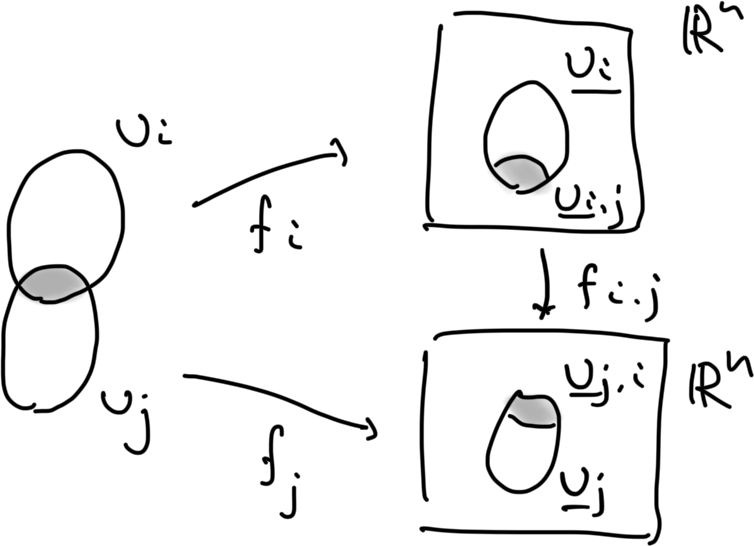
\includegraphics[scale=.3]{mfd.png} \]
\caption{Coordinate patches of a manifold \label{fig:coord-patch}}
\end{figure}

Suppose $U_i\cap U_j$ is nonempty. 
Let \begin{align}
\underline{U}_{i,j} &:= f_i(U_i\cap U_j) \subset \underline{U}_i,\\
\underline{U}_{j,i} &:= f_j(U_j\cap U_i)\subset \underline{U}_j.
\end{align}
Then we have the map \begin{equation}
f_{i,j} \colon \underline{U}_{i,j} \to \underline{U}_{j,i} 
\end{equation} defined by \begin{equation}
f_{i,j} := f_j \circ (f_i)^{-1} .
\end{equation}
This allows us to `paste together' $\underline{U}_i\subset \bR^n$ 
and $\underline{U}_j \subset \bR^n$
by identifying their subsets $\underline{U}_{i,j}$ and $\underline{U}_{j,i}$ using $f_{i,j}$.
%See Fig.~\ref{fig:pasting} for a drawing.


A smooth manifold is such that $f_{ij}$ are smooth;
a topological manifold is such that $f_{ij}$ are just required to be continuous.
A smooth manifold is automatically a topological manifold.
A bijective smooth map $f:M\to M'$ between two smooth manifolds $M$ and $M'$
is called a \emph{diffeomorphism};
a bijective continuous map $f:M\to M'$ between two topological manifolds $M$ and $M'$
is called a \emph{homeomorphism}.
In physics we typically consider smooth manifolds,
but I decided to include a bit of discussions about topological manifolds
as I thought the subtle concrete differences between smooth manifolds
and topological manifolds can be interesting to some of you.

\begin{theorem}
When a manifold $M$ is compact,
we can choose a finite number of coordinate patches $U_i$ to cover $M$.
\end{theorem}

Before going further, let us also introduce manifolds with boundaries:
\begin{definition}
  A \emph{manifold with boundary} is defined similarly,
  but we allow the neighborhood $\underline{U}$ to be in a half-space $\bR^{n-1}\times \bR_{\ge 0}$.
  The union of the inverse images of the boundary of 
  $\underline{U}\cap (\bR^{n-1} \times \{0\})$ 
  under $f$ is called \emph{the boundary of $M$}
  and is denoted by $\partial M$.
\end{definition}  

\begin{example}
  The half-space $\bR^{n-1}\times \bR_{\ge 0}$ is a manifold with boundary.
\end{example}

\begin{definition}
  A compact manifold without boundary is called a closed manifold.
\end{definition}


\subsection{Manifolds via equations}
So far we only saw trivial examples.
We need better examples.

\subsubsection{Generalities}
A common way to construct manifolds is to take a subset of $\bR^n$ defined by a number of equations:
\begin{align}
f_1(x_1, x_2, \ldots, x_n) &= 0, \\
f_2(x_1, x_2, \ldots, x_n) &= 0, \\
&\vdots \\
f_m(x_1, x_2, \ldots, x_n) &= 0.
\end{align}
If the choice of $f_{1,2,\ldots,m}$ are sufficiently nice,
the set of points satisfying these equations is a manifold of dimension $n-m$.

A typical bad example is the subset of $\bR^2$ defined by $xy=0$: around $(x,y)=(0,0)$, two lines intersect, and therefore the neighborhood of $(0,0)$ is not of the right form.

\subsubsection{Spheres and disks/balls}

\begin{example}
The $n$-dimensional sphere $S^n$ is defined by \begin{equation}
  x_1^2+x_2^2+\cdots+x_{n+1}^2=1.
\end{equation} 
\end{example}
Note that $S^n$ is embedded in $\bR^{n+1}$, but it is a manifold of dimension $n$.

\begin{example}
  The $n$-dimensional disk $D^n$ is defined by \begin{equation}
    x_1^2+x_2^2+\cdots+x_{n}^2\le 1.
  \end{equation} 
  This is a manifold with boundary, and the boundary is $S^{n-1}$.
  $D^n$ also called the $n$-dimensional ball and denoted by $B^n$.
\end{example}  

\begin{example}
$D^1$ is a segment $[-1,1]$ and its boundary $S^0$ consists of two points $\{-1,1\}$.
\end{example}

Calling two points, $S^0$, a 0-dimensional sphere sounds silly,
but it is just a name.
But this illustrates an important point:
you are not supposed to judge mathematical concepts by their names.
Rather, you are supposed to understand them by internalizing their definitions into your heart.

\begin{example}
  We can try considering points of constant Lorentz-invariant distance from the origin in $\bR^{d-1,1}$:
\begin{equation}
  x_1^2+x_2^2+\cdots+x_{d-1}^2-x_0^2=K ,
\end{equation}
where $K$ is a non-zero constant. 
This is a hyperboloid, and is a manifold of dimension $d-1$.
\end{example}
When $K>0$, it is connected; this is the hypersurface of spacelike-separated points 
of distance $\sqrt{|K|}$ from the origin
in the Minkowski spacetime.
When $K<0$, it consists of two components, one in the future $x_0>0$ and another in the past $x_0<0$.
They are the hypersurfaces of time-like separated points of temporal distance $\sqrt{|K|}$ from the origin.
When $K=0$, the equation above defines the lightcone, which is singular at the origin and is not a manifold.

\subsubsection{Group manifolds}
We have various group manifolds, 
defined in a similar manner.
 
Let $M_n(\bR)$ be the set of $n\times n$ real matrices.
\begin{example}
The orthogonal group $O(n)$ is defined by \begin{equation}
  O(n) = \{ M\in M_n(\bR) \mid M^T M = 1 \}.
\end{equation}
The special orthogonal group $SO(n)$ is defined by \begin{equation}
  SO(n) = \{ M\in O(n) \mid \det M = 1 \}.
\end{equation}
\end{example}

Similarly let $M_n(\bC)$ be the set of $n\times n$ complex matrices.
\begin{example}
The unitary group $U(n)$ is defined by \begin{equation}
  U(n) = \{ M\in M_n(\bC) \mid M^\dagger M = 1 \}.
\end{equation}
The special unitary group $SU(n)$ is defined by \begin{equation}
  SU(n) = \{ M\in U(n) \mid \det M = 1 \}.
\end{equation}
\end{example}

\begin{proposition}
$S^1=U(1)=SO(2)$.
\end{proposition}
This can be seen by parameterizing $S^1$ by $\theta \in [0,2\pi)$.
$U(1)$ is a one-by-one unitary matrix, i.e.~a complex number $z$ with $|z|=1$.
Therefore $z=e^{i\theta}$.
$SO(2)$ is a two-by-two orthogonal matrix with determinant $1$, which has the form \begin{equation}
  \begin{pmatrix}
    \cos\theta & -\sin\theta \\
    \sin\theta & \cos\theta
  \end{pmatrix}.
\end{equation}

\begin{proposition}
$S^3=SU(2)$.
\end{proposition}
This can be seen by noticing that any $SU(2)$ matrix has the form \begin{equation}
  \begin{pmatrix}
    z & -\overline w\\
    w & \overline z
  \end{pmatrix}
\end{equation} with $|z|^2+|w|^2=1$.
As $\bC^2\simeq \bR^4$, we see that this defines an $S^3$.
This fact can also be shown using quaternions $\bH$, 
introduced by Hamilton in 1843.
\begin{definition}
$\bH$ is a four-dimensional algebra over $\bR$ with a basis $1,i,j,k$ satisfying \begin{equation}
  i^2=j^2=k^2=-1, \quad
  ij=-ji=k, \quad
  jk=-kj=i, \quad
  ki=-ik=j.\label{eq:rel-of-H}
\end{equation}
\end{definition}

A general element is of the form $q=a+bi+cj+dk$ with $a,b,c,d\in \bR$.
The conjugate of $q=a+bi+cj+dk$ is $\bar q=a-bi-cj-dk$.
We can check that $\overline{q_1 q_2}=\bar q_2 \bar q_1$.

The norm of $q$ is $|q|^2=q\bar q=\bar q q=a^2+b^2+c^2+d^2$.
This is nonzero unless $q=0$.
This means that any nonzero element $q\neq 0$ has a multiplicative inverse $q^{-1}=\bar q/|q|^2$.
An algebra with this property is called a division algebra.
\begin{fact}
  The only finite-dimensional division algebras over $\bR$ are $\bR$, $\bC$, and $\bH$.
\end{fact}

Note also that $|q_1 q_2|^2=|q_1|^2 |q_2|^2$.
This means that the set $\{ q\in \bH \mid |q|=1 \}$ of unit quaternions forms a group.
As $\bH\simeq \bR^4$, this is a three-dimensional sphere $S^3$.
Considering $\bH\simeq \bC^2$, we can convince ourselves that this is also $SU(2)$.
More generally:
\begin{example}
  The unitary symplectic group $Sp(n)$ is defined by \begin{equation}
    Sp(n) = \{ M\in M_{n}(\bH) \mid M^\dagger M = 1 \}.
  \end{equation}
\end{example}
In particular, $Sp(1)=SU(2)=S^3$.
Note there is no distinct `special unitary symplectic group'.

To explain $Sp(m)$ a bit more geometrically, consider $\bH^n$
as the space of column vectors of quaternions. 
We consider `linear' maps  $M:\bH^n\to \bH^n$ in the sense that
\begin{equation}
M (vq) = (Mv) q, \qquad v\in \bH^n,\ q\in \bH.
\end{equation} 
(Note that the placement of $q$ on the right is important, 
as the multiplication is non-commutative in $\bH$.)
Denote the basis vectors by $e_1,e_2,\ldots,e_n$.
Then such an $M$ is specified by \begin{equation}
M e_i = \sum_j M_{ij} e_j.
\end{equation}
The condition $M^\dagger M=1$ is the condition that it preserves the norm $|v|$ of $v\in \bH^n$
defined by \begin{equation}
  |v|^2 := \sum_i |v_i|^2.
\end{equation}

\begin{fact}
  The only cases when $S^n$ is a group are $S^0=O(1)=\{1,-1\}$, $S^1=SO(2)=U(1)$
  and $S^3=SU(2)=Sp(1)$.
\end{fact}

Before moving on,
we also introduce the notations:
\begin{definition}
We use the notation $GL(n,\bK)$ for the group of invertible $n\times n$ matrices over a field $\bK$.
\end{definition}

\subsubsection{Aside: time reversal and $\bR$, $\bC$, $\bH$}

Let me make a side remark concerning the natural role of $\bH$ in quantum mechanics.
Let's consider a quantum mechanical system with finite-dimensional Hilbert space $\cH$.
The time reversal operator $\sT$ is anti-unitary, in that 
\begin{equation}
  \sT z = \overline z \sT.
\end{equation}
Assuming that $\sT^2=c$ with a constant $c$, let's show $c=\pm1$. We evaluate $\sT^3$ in two orders:
\begin{equation}
\sT(\sT^2)= \sT c = \overline{c}\sT,\qquad
(\sT^2)\sT = c\sT.
\end{equation} Therefore $c=\overline{c}$. As the unitarity of $\sT^2$ requires $|c|=1$,
 we find $c=\pm 1$.

 \paragraph{The case $c=+1$:}
 This case, any vector $v\in \cH$ can be decomposed into its real and imaginary parts:
  \begin{equation}
    v = v_\text{re} + v_\text{im} i 
  \end{equation}
  where
  \begin{equation}
    v_\text{re}:= \frac{1+\sT}{2} v, \quad v_\text{im}:=\frac{1-\sT}{2i}v .
  \end{equation}
  Note that $T v_\text{re}= v_\text{re}$ and $T v_\text{im}=v_\text{im}$.
So, the $T$-invariant part of $\cH$ is a real vector space.
Denoting it by $\cH_\bR$, we see that if $\cH_\bR=\bR^n$, $\cH=\bC^n$.
Unitary matrices acting on $\cH$ commuting with $\sT$
are orthogonal matrices acting on $\cH_\bR$.
So, time-reversal-invariant unitary operators on $\cH$ 
form the group $O(n)$.

\paragraph{The case $c=-1$:}
In this case, we note that $i$, $j:=\sT$, $k:=i \sT$ satisfy 
the defining relation \eqref{eq:rel-of-H} of $\bH$.
(More precisely, we can equip the space $\cH$ of quantum states
with an action of $\bH$ from the right, via $vi := iv$ and $vj:=\sT v$.)

Therefore, $\cH= \bH^m$ for some $m$. When $\cH=\bC^n$, this forces $n=2m$ to be even.
This is known as Kramers degeneracy.

A unitary operator commuting with $\sT$
is a norm-preserving map on $\bH^m$ which commutes with the quaternion action from the right.
Therefore it belongs to $Sp(m)$.

\paragraph{Summary:}
$U(n)$, $SO(n)$, and $Sp(n/2)$ are the groups of norm-preserving linear operators
on a quantum system $\cH=\bC^n$ with $n$ states with the following conditions:
\begin{itemize}
\item $U(n)$: no time reversal,
\item $SO(n)$: time reversal with $\sT^2=+1$,
\item $Sp(n/2)$: time reversal with $\sT^2=-1$; $n$ is forced to be even.
\end{itemize}


\subsection{Manifolds via combinations}

Let's come back to the examples of manifolds.

\begin{notation}
 Given two manifolds $M$ and $N$ of dimensions $m$ and $n$,
 we write its product as $M\times N$.
It is a manifold of dimension $m+n$.
\end{notation}

\begin{notation}
Given two manifolds $M$ and $N$ of the same dimension $n$,
we write its disjoint union as $M\sqcup N$.
It is a manifold of dimension $n$.
\end{notation}

Note that $S^1\times S^1$ is two-dimensional and the surface of a donut,
while $S^1\sqcup S^1$ consists of two circles and is one-dimensional.

\begin{example}
  The $n$-dimensional torus is \begin{equation}
    T^n = \underbrace{S^1\times S^1\times \cdots \times S^1}_\text{ $n$ times}.
  \end{equation}
\end{example}

\begin{example}
$S^1\times [-1,1]$ is a cylinder. Its boundary is $S^1\sqcup S^1$.
\end{example}

Another construction is the following:
\begin{notation}
  Given two connected manifolds $M$, $N$ of dimension $n$,
  pick points $p\in M$ and $q\in N$.
  remove small open balls $B^n(p)$ and $B^n(q)$ from $M$ and $N$, and
  paste the common $S^{n-1}$ boundary.
  The result is the connected sum $M\# N$.
\end{notation}

For example, the connected sum 
\begin{equation}
  \underbrace{T^2 \# T^2 \# \cdots \# T^2}_\text{$g$ copies}
\end{equation}
is the surface of a multi-donut (whatever that is).
More professionally, it is called a genus-$g$ surface.
$S^2$ is defined to have genus 0.

\begin{fact}
Any two-dimensional compact connected oriented manifold is $S^2$ or 
the surface of a multi-donut with $g$ holes.
\end{fact}

\subsection{Manifolds via quotients}
\label{sec:quotient}
\subsubsection{Generalities}
Another method to define manifolds is to 
take the quotient of a manifold by a group action. 
Let us explain it more fully.
\begin{definition}
A \emph{group action} of a group $G$ on a manifold $M$ is a map \begin{equation}
  M\times G \to M, \quad (p, g) \mapsto p q
\end{equation} such that \begin{equation}
   p e = p, \quad  (p  g) h = p (gh)
\end{equation} for all $g,h\in G$ and $p\in M$.
Here $e$ is the identity in $G$.
We often abbreviate this situation by writing $M \curvearrowleft G$.
\end{definition}

More precisely, this is known as a right action of $G$.
We can similarly define a left action of $G$, so that 
we have $G\times M\to M$ satisfying $g(hp)=(gh)p$ instead.
We write $G\curvearrowleft M$ in this case.
In either case, we usually want the action to be smooth or at least continuous,
depending on the context.

Representations of groups on vector spaces are special cases:
\begin{definition}
  A representation $\rho$ of a group $G$ on a $\bK$-vector space $V$ is a group action (from the left) of $G$ on $V$, commuting with the scalar multiplication by $\bK$ (from the right).
  This means that for each $g\in G$, we have linear maps $\rho(g):V\to V$ such that $\rho(gh)=\rho(g)\rho(h)$.    
  We often abbreviate this situation by writing $\rho: G\curvearrowright V$.
\end{definition}

Let us now define the quotients:
\begin{definition}
For $p,q\in M$, let $p\sim q$ if there is a $g\in G$ such that $p g = q$.
The quotient space $M/G$ is the set $M/\sim$ of equivalence classes 
under this relation.
\end{definition}

$M/G$ is not always a manifold.
For example, consider $\bR^3$ with the action of $\bZ_2$ generated by 
\begin{equation}
(x,y,z) \mapsto (-x,-y,-z).
\end{equation}
The origin is singular, and the quotient space $\bR^3/\bZ_2$ is not a manifold.
(It still belongs to a larger class of spaces called \emph{orbifolds}.)
Actually, the quotient of a vector space by a group via its representation is almost never a manifold.
It is complicated to state the conditions under which $M/G$ is a manifold,
so we will not do so in this lecture series.

\subsubsection{Projective spaces}
We now define the real, complex and quaternionic projective spaces $\RP^n$, $\CP^n$ and $\HP^n$ uniformly.
\begin{example}
  \label{ex:proj}
  For $\bK=\bR,\bC,\bH$, 
  consider the action of $\bK\setminus \{0\}$ on
  $\bK^{n+1}\setminus\{0\}$ by scalar multiplication, (from the right when $\bK=\bH$).
  The projective space $\KP^n$ is then defined as
  \begin{equation}
    \KP^n = (\bK^{n+1}\setminus\{0\})/(\bK\setminus\{0\}).
  \end{equation}
  These are of dimension $n$, $2n$, and $4n$ respectively.
\end{example}
More directly, we consider elements 
\begin{equation}
(x_1,x_2,\ldots,x_{n+1})\in \bK^{n+1}
\end{equation} such that not all of $x_i$ is zero.
Then we make the identification \begin{equation}
  (x_1,x_2,\ldots,x_{n+1}) \sim  ( x_0, x_1, \ldots,  x_n)c \label{eq:proj-ident}
\end{equation} for nonzero $c\in \bK$.
A point on $\KP^n$,
which is an equivalence class under \eqref{eq:proj-ident},
is often denoted by \begin{equation}
  [x_1:x_2:\cdots:x_{n+1}].
\end{equation}


It is instructive to give explicit coordinate patches.
Let $U_i$ be the points on $\CP^n$ with $x_i\neq 0$.
Note that when $x_i\neq 0$, we have \begin{equation}
  (x_1,x_2,\ldots,x_{n+1}) \sim (x_1/x_i, x_2/x_i, \ldots, x_i/x_i=1, \ldots, x_{n+1}/x_i).
\end{equation} 
In other words, we can introduce coordinates on $U_i$ by defining  $y_k:=x_k/x_i$ for $k\neq i$;
equivalently, we constructed a map $f_i: U_i \to \underline{U}_i \simeq \bK^n$.

Let us consider another patch $U_j$ containing points with $x_j\neq 0$. 
We introduce coordinates $z_k:=x_k/x_j$ for $k\neq j$;
this gives the map $f_j: U_j \to \underline{U}_j\simeq \bK^n$.

$U_i$ and $U_j$ overlap when $x_i\neq 0$ and $x_j\neq 0$.
We then need to find the coordinate transformation 
between $f_i(U_i \cap U_j )\subset \underline{U}_i$
and $f_j(U_i \cap U_j) \subset \underline{U}_j$, realizing the identification of
\begin{equation}
  (y_1,y_2,\ldots,y_{n+1}) \quad \text{with $y_i=1$, $y_j\neq 0$}
\end{equation} and 
\begin{equation}
  (z_1,z_2,\ldots,z_{n+1}) \quad \text{with $z_j=1$, $z_i\neq 0$}.
\end{equation}
This is done by setting $z_k = y_k / y_j$, where $y_i$ was defined to be $=1$.

From this description we see \begin{equation}
\RP^1=S^1,\quad
\CP^1=S^2,\quad
\HP^1=S^4.
\label{eq:KP1}
\end{equation}
Indeed, in this case we have two patches \begin{equation}
  U_1 = \{ [1:y] \mid y\in \bK \}, \quad U_2 = \{ [z:1] \mid z\in \bK \}.
\end{equation} where $z=y^{-1}$ in the overlap $U_1\cap U_2$.
$U_1$ is the northern hemisphere,
$U_2$ is the southern hemisphere,
and they are patched to form a sphere in the appropriate dimensions.

Another way to look at $\KP^n$ is the following. 
To pick a representative under the identification \eqref{eq:proj-ident},
we first fix $\sum_i |x_i|^2 =1$.
As $\bK^{n+1}=\bR^{p(n+1)}$ where $p=1,2,4$ for $\bK=\bR,\bC,\bH$,
we have $S^n$, $S^{2n+1}$, $S^{4n+3}$ at this point.

The identification \eqref{eq:proj-ident} still acts within this sphere
if $|c|=1$. 
Depending on $\bK=\bR,\bC,\bH$, the group of such $c$ is $O(1)=\{\pm1\}=S^0$, $U(1)=S^1$, $Sp(1)=SU(2)=S^3$, respectively.
Therefore, we have \begin{proposition}
\label{prop:sphere-proj}
$\RP^n=S^n/O(1), \quad \CP^n=S^{2n+1}/U(1), \quad \HP^n=S^{4n+3}/Sp(1)$.
\end{proposition}

\begin{remark}
Before proceeding, we note that $\CP^n$ parameterize physically-distinct pure states 
in an $(n+1)$-dimensional Hilbert space.
Indeed, two nonzero ket vectors $\ket{\psi}$ and $\ket{\psi'}$ represent the same physical state
when there is a complex number $c$ such that $\ket{\psi'}=c\ket{\psi}$.
This is exactly the condition \eqref{eq:proj-ident}.
\end{remark}


\subsubsection{Homogeneous spaces}
\label{sec:homogeneous}
\paragraph{Generalities:}
Another large class of quotient spaces
are the homogeneous spaces.
\begin{definition}
  \label{def:homogeneous-space}
  Given a subgroup $H\subset G$,
  introduce the equivalence relation $g_1\sim g_2$ if 
  there exists an $h\in G$ such that $g_1=g_2 h$.
  The quotient of $G$ by this relation is denoted by $G/H$,
  and is called a homogeneous space.
\end{definition}

A common way homogeneous spaces appear in physics is via symmetry breaking.
Say we have a configuration space $M$ (typically a vector space) acted on by a symmetry group $G$ from the left:
$M\ni m\mapsto gm\in M$ for $g\in G$.
Suppose we have a potential (or a free energy) $V:M\to \bR$ invariant under the $G$ action, i.e.~$V(gm)=V(m)$.
Suppose further that the potential has a minimum at $m_0 \in M$. 
From the $G$-invariance, all points of the form $gm_0$ are also minimum of $V$.
When the potential is generic, the space of the minimum of the potential is given by the orbit $Gm_0$.
Can we say more about the structure of this space?

Let $H\subset G$ be the subgroup fixing $m_0$, i.e.~$h\in H$ if and only if $hm_0=m_0$.
In such a situation, we say that the symmetry is broken from $G$ to $H$.\footnote{%
Physicists often write this as $G\to H$, 
but mathematically the map is in the opposite direction, $H\to G$.}
In this case $g_1 m_0 = g_2 m_0$ if and only if $g_2^{-1} g_1 \in H$, 
or equivalently $g_1 = g_2 h$ for some $h\in H$.
Therefore, we have $Gm_0=G/H$, i.e.~the space of the potential minimum is a homogeneous space
determined by the original symmetry $G$ and the unbroken symmetry $H$.

Note that mathematicians call the subgroup $H$ as the stabilizer of $m_0$,
whereas physicists usually call it the unbroken subgroup.

\paragraph{Wine bottle potential:}
Let us give some examples.
We start with two trivial examples.
Let $G=SO(2)$ act on $(x,y)\in \bR^2$ by rotations.
A rotationally invariant potential $V(x,y)$ has the form
$V(x,y)=f(r)$ for $r^2=x^2+y^2$.
When the minimum is at $(x,y)=(0,0)$, its orbit under $SO(2)$ is a single point, $\{(0,0)\}$.
In this case the unbroken subgroup $H$ is the entirety of $SO(2)$.
So, we have $SO(2)/SO(2)=\{\text{point}\}$, a zero dimensional manifold consisting of a single point.
It is often abbreviated as $\pt$ in algebraic topology, so $SO(2)/SO(2)=\pt$.

When the minimum is at $(x,y)=(r_0,0)$ with $r_0\neq 0$,
its orbit under $SO(2)$ is the circle of radius $r_0$.
In this case the unbroken subgroup $H$ is $\{e\}$,
and $SO(2)/\{e\}=SO(2)$, which is a circle.
For an illustration, see Fig.~\ref{fig:winebottle}.

\begin{figure}[h]
\centering
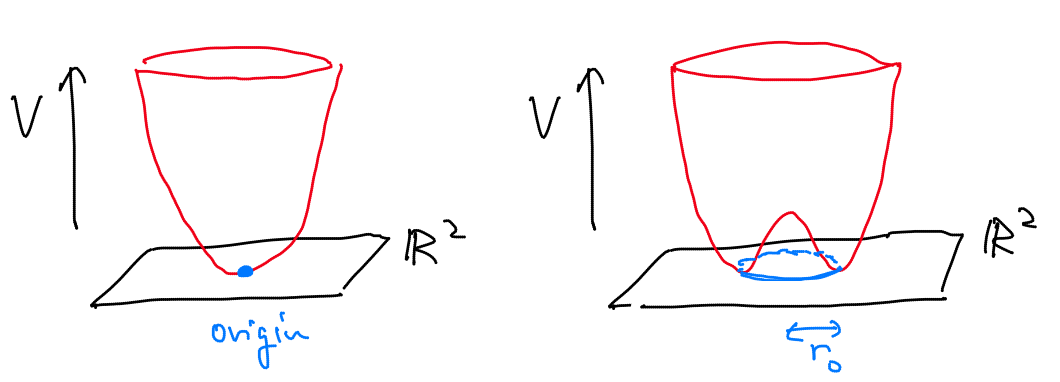
\includegraphics[width=.7\textwidth]{winebottle.png}
\caption{Two choices of $SO(2)$-invariant potential functions $V(x,y)$,
with minimum either at the origin or at the circle of radius $r_0$.}
\label{fig:winebottle}
\end{figure}

\paragraph{Generalized wine bottles:}
Let us generalize.
Let $SO(n)$ act on $\bR^n$ by rotations.
A rotationally invariant potential $V:\bR^n\to \bR$ 
has the form $V(x_1,\ldots,x_n)=f(r)$ where $r^2={x_1^2+\cdots+x_n^2}$.
When $f(r)$ has a minimum at $r_0>0$,
the space of the potential minimum is $S^{n-1}$ given by $x_1^2+\cdots + x_n^2=r_0^2$.

At $m_0=(r_0,0,\ldots,0)$, the subgroup of $SO(n)$ fixing $m_0$ is $SO(n-1)$.
Therefore, the space of the potential minimum is $SO(n)/SO(n-1)=S^{n-1}$.
Summarizing, we have found
\begin{proposition}
  \label{prop:SO/SO}
 $ SO(n)/SO(n-1) \simeq S^{n-1}$.
\end{proposition}

Let $U(n)$ act on $\bC^n$ by unitary transformations.
An invariant potential $\bC^n\to \bR$ has the form $V(z_1,\ldots,z_n)=f(r)$
where $r^2=|z_1|^2+\cdots+|z_n|^2$.
When $f(r)$ has a minimum at $r_0>0$,
the space of the potential minimum is $S^{2n-1}$ given by $|z_1|^2+\cdots + |z_n|^2=r_0^2$.

At $m_0=(r_0,0,\ldots,0)$, the subgroup of $U(n)$ fixing $m_0$ is $U(n-1)$.
Therefore, the space of the potential minimum is $U(n)/U(n-1)=S^{2n-1}$.
\begin{proposition}
  \label{prop:U/U}
$U(n)/U(n-1)\simeq S^{2n-1}$.
\end{proposition}

Let $Sp(n)$ act on $\bH^n$ in a standard manner.
By following the same logic as above, we get $Sp(n)/Sp(n-1)=S^{4n-1}$,
and we found that:
\begin{proposition}
  \label{prop:Sp/Sp}
$ Sp(n)/Sp(n-1)\simeq S^{4n-1}$.
\end{proposition}

\paragraph{Observables in quantum mechanics:}
Let us discuss a different but common example we see in quantum mechanics.
Consider an $n$-state system with the Hilbert space $\cH=\bC^n$.
The unitary group $U(n)$ acts on it.
On the observables, $g\in U(n)$ acts via \begin{equation}
  A\mapsto g A g^\dagger.
\end{equation}
Therefore, the subgroup $U(1) \subset U(n)$
consisting of scalar multiplications acts trivially: \begin{equation}
c A c^\dagger = A,
\end{equation} when $|c|=1$. 
What acts effectively on the space of observables is the quotient group $U(n)/U(1)$.

We note that $SU(n)\subset U(n)$ also acts on observables.
In this case, a scalar multiplication $c$ with $|c|=1$ is in $SU(n)$ if and only if $c^n=1$.
The complex numbers $\{c\mid c^n=1\}$ form a group isomorphic to $\bZ_n$,
and we found $\bZ_n \subset SU(n)$,
and the quotient $SU(n)/\bZ_n$ acts on the space of observables.

As any $U(n)$ matrix $U$ is of the form $c'U'$ for $c'\in U(1)$ and $U'\in SU(n)$,
we have $U(n)/U(1) = SU(n)/\bZ_n$.
This common quotient group is known as the projective unitary group, and denoted by $PU(n)$.
Summarizing, 
\begin{example}
The common quotient $U(n)/U(1)=SU(n)/\bZ_n$ is called the projective unitary group and is denoted by $PU(n)$.
\end{example}

For those who take wavefunctions as supreme, the natural symmetry group is $U(n)$,
whereas for those who take density matrices and/or observables as supreme,
the natural symmetry group is $PU(n)$.
This difference can produce subtle topological effects,
as we will see during this lecture series.

\paragraph{Chiral symmetry breaking in QCD:}
As our next example, 
let us consider the chiral symmetry breaking in QCD.
For simplicity let us consider the two-flavor case.
The symmetry $G$ is $SU(2)\times SU(2)$,
which acts on $\bC^2 \otimes \bC^2$,
where two $\bC^2$ factors are the standard two-dimensional representations of $SU(2)$.
A more convenient way to think about this action
is to regard $\bC^2\otimes \bC^2$ as the space of 
complex two-by-two matrices $M_2(\bC)$,
and to let $(g,g')\in SU(2)\times SU(2)$ to act on $m\in M_2(bC)$
via \begin{equation}
m\mapsto g m g'{}^{-1}.
\end{equation}

Say that $m$ takes the value $m=\mathbf{1}_{2\times 2}$.
The unbroken subgroup $H$ is formed by 
$\{(g,g)\}\subset SU(2)\times SU(2)$,
which is isomorphic to $SU(2)$ and is called the diagonal subgroup.
The orbit of $\mathbf{1}_{2\times 2}$ is simply 
the matrices of the form $gg'$,
i.e.~the subspace $SU(2)\subset M_2(\bC)$.
We thus found:
\begin{proposition}
We have $SU(2)\times SU(2)/SU(2)_\text{diagonal} = SU(2)$.
\end{proposition}

\paragraph{Superfluid $^3$He:}
Our final example is the superfluid $^3$He;
its theory can be learned e.g.~in \cite{SuperfluidHe3Textbook,VolovikBook}.
It has a phase diagram as given in Fig.~\ref{fig:3He}.
\begin{figure}[h]
\centering
    \includegraphics[width=0.6\textwidth]{3He.pdf}
    \caption{Phase diagram of $^3$He (taken from \cite[Fig.7.1]{VolovikBook}).}
    \label{fig:3He}
\end{figure}
A $^3$He atom is a fermion with spin $1/2$, which can form a Cooper pair at low temperature.
There are two superfluid phases with zero magnetic field, known as the A phase and the B phase.
The order parameter (the expectation value of the Cooper pair) takes values in
$\bC^3\otimes \bC^3$,
where the first factor is for the spin angular momentum
and the second factor is for the orbital angular momentum,
both with spin 1.
Denote the basis vectors of the first $\bC^3$ by $\mathbf{e}_{1,2,3}$
and those of the second by $\mathbf{f}_{1,2,3}$.
The symmetry group $G$ of the free energy (neglecting a small spin-orbit coupling) is given by two separate $SO(3)$ actions on 
$\mathbf{e}_{1,2,3}$ and $\mathbf{f}_{1,2,3}$,
together with a common $U(1)$ phase rotation $\mathbf{e}_i \otimes \mathbf{f}_j \mapsto c\, \mathbf{e}_i \otimes \mathbf{f}_j$.
Therefore, we have \begin{equation}
  G = SO(3)\times SO(3)\times U(1)
\end{equation}
as the symmetry of the free energy.
\begin{example}
\label{ex:helium3}
In the superfluid phases of $^3$He, the order parameter takes the value
\begin{itemize}
\item $\mathbf{e}_1 \otimes (\mathbf{f}_2+ i\mathbf{f}_3)$ in the A phase,
\item $\sum_i \mathbf{e}_i \otimes \mathbf{f}_i$ in the B phase.
\end{itemize}
Denoting the subgroup preserved by these order parameters by $H_\text{A,  B}$,
the space of the potential minimum is given by $G/H_\text{A}$, $G/H_\text{B}$, respectively.
\end{example}

\begin{question}
Describe $H_\text{A}$ and $H_\text{B}$ as explicitly as possible.
\end{question}
You will see that the pattern of symmetry breaking is very similar to the 
breaking of the chiral symmetry in QCD.

With magnetic field, there is also a phase known as the A$_1$ phase.
The magnetic field reduces the symmetry of the free energy
to $SO(2)\times SO(3)\times U(1)$
and the order parameter takes the value 
 $(\mathbf{e}_2+i\mathbf{e}_3) \otimes (\mathbf{f}_2+ i\mathbf{f}_3)$.

We have one final question before moving on:
\begin{question}
Projective spaces are homogeneous spaces. Could you describe them as such?
\end{question}


\subsection{Non-orientable surfaces}

Let us now discuss some non-orientable manifolds.

\begin{example}
  Consider $S^1\times [-1,1]$, parameterized by $\theta\sim \theta+2\pi$ and $x\in [-1,1]$.
  We can consider the $\bZ_2$ action $(\theta,x)\mapsto (\theta+\pi,-x)$.
  The quotient space is called the M\"obius strip.
  This is non-orientable, and the boundary is a single circle $S^1$.
\end{example}

As a non-orientable closed manifold, 
we have $\RP^2$ we introduced above. To see this, recall $\RP^2=S^2/\bZ_2$,
where the $\bZ_2$ action identifies the antipodal points. 
Any point on the southern hemisphere is identified with some point on the northern hemisphere.
Then $\RP^2$ can be identified with the northern hemisphere
whose boundary, i.e.~the equator, has an extra identification $\theta \sim \theta+\pi$.

Let us have a closer look at the neighborhood of the equator.
We can parameterize it by the longitude $\theta$ together with the latitude $\phi\in (-\epsilon,\epsilon)$.
The antipodal identification is $(\theta,\phi)\sim (\theta+\pi,-\phi)$.
This is the same as the M\"obius strip, which is non-orientable.
In string theory, this local structure around the equator is called a crosscap (叉帽).
Another way to say this is that $\RP^2$ is obtained by pasting a northern hemisphere (i.e.~a disk)
to a M\"obius strip along the boundary.
Summarizing,
\begin{proposition}
$\RP^2$ is non-orientable.
\end{proposition}

Another non-orientable surface can be constructed by the following quotient:
\begin{example}
Consider $T^2$ parameterized by $\theta$ and $\phi$
with the identification $\theta\sim \theta+2\pi$ and $\phi \sim \phi+2\pi$,
and take a further identification as above: $(\theta,\phi)\sim (\theta+\pi,-\phi)$.
The result is known as the Klein bottle.
\end{example}
Locally around $\phi=0$ and $\phi=\pi$, we have two M\"obius strips.
So the resulting surface is obtained by pasting two M\"obius strips along the boundary.
Equivalently, it is obtained by taking the connected sum $\RP^2\#\RP^2$.

We can consider many other non-orientable surfaces by taking a repeated connected sum:
\begin{equation}
  \underbrace{\RP^2\#\RP^2\#\cdots\#\RP^2}_\text{$h$ copies}
  \#
  \underbrace{T^2\# T^2 \#\cdots\# T^2}_\text{$g$ copies}
\end{equation}
where we take $h>0$ and $g\ge 0$.
In fact, many of them are actually homeomorphic to each other.
\begin{fact}
Any compact connected non-orientable 2d surface is homeomorphic to
\begin{equation}
\RP^2 \# \underbrace{T^2\# T^2 \#\cdots\# T^2}_\text{$g$ copies}
\end{equation}
or the Klein bottle $\RP^2\#\RP^2$.
\end{fact}
It is a fun exercise to show that $\RP^2 \# \RP^2 \# \RP^2$ is homeomorphic to $\RP^2 \# T^2$.

\subsection{Aside: some other fun manifolds}


\subsubsection{The de-singularization of $\bC^2/\bZ_2$}
Let's consider $\bC^2$ parameterized by $(z,w)$,
and consider the $\bZ_2$ action $(z,w)\mapsto (-z,-w)$.
The quotient space $\bC^2/\bZ_2$ is singular at the origin.
We can parameterize the same space in a different way:
Let $(s,t,u):=(z^2, z w, w^2)$.
Then the $\bZ_2$ action is trivial on $(s,t,u)$, but we have the relation $su=t^2$.
From $(s,t,u)$ satisfying $su=t^2$, we can uniquely reconstruct $(z,w)\simeq -(z,w)$.
So $\bC^2/\bZ_2$ can be identified with the subspace \begin{equation}
X=\{ (s,t,u)\in \bC^3 \mid su=t^2 \}.
\end{equation}
We can desingularize $X=\bC^2/\bZ_2$ in the following way.

We add the variables $(x_1,x_2)\in \bC^2\setminus \{0\}$, with the identification 
$(x_1,x_2)\sim a(x_1,x_2)$ for $a\in \bC\setminus \{0\}$,
i.e.~we introduce $\CP^1\simeq S^2$.
Recall that its points are denoted by $[x_1:x_2]$.
We now add a further constraint \begin{equation}
(z,w) = c(x_1,x_2) \quad \text{for some $c\in \bC$},
\end{equation} or equivalently \begin{equation}
  (s,t,u)= c'(x_1^2, x_1 x_2, x_2^2) \quad \text{for some $c'\in \bC$}. \label{eq:blowup}
\end{equation}

Denote the total space by $\tilde X$: 
it is a subspace of $\bC^3\times \CP^1$ 
parameterized by 
$(s,t,u,[x_1:x_2])$ 
under the constraints $su=t^2$ and \eqref{eq:blowup}.
This space comes with two projections maps, $\pi_1:\tilde X\to X=\bC^2/\bZ_2$ 
given by taking $(s,t,u)$
and $\pi_2:X\to \CP^1$ given by taking $[x_1:x_2]$.

Note that $\pi_1$ is one-to-one except at the origin, $(z,w)=(0,0)$.
It is because the relation \eqref{eq:blowup} uniquely determines $[x_1:x_2]=[z:w]$.
At the origin, $(z,w)=(0,0)$, the inverse image is the entirety of $\CP^1$. 
So, $\tilde X$ can be thought of inserting  $\CP^1$ at the origin of $X=\bC^2/\bZ_2$.

$\tilde X$ is actually a smooth manifold.
To see this, we consider the second projection $\pi_2: \tilde X\to \CP^1$.
Given a point $[x_1:x_2]\in \CP^1$,
the inverse image of $\pi_2$ is simply $c'(x_1^2, x_1 x_2, x_2^2)\in \bC$
for $c'\in \bC$. 
So it is isomorphic to a copy of $\bC$.
So $\tilde X$ can be visualized as a copy of $\bC$ attached smoothly at each point of $\CP^1$,
and is a smooth manifold.
This is an example of a fiber bundle we discuss in the next section.

\subsubsection{A K3 manifold}

The manifold $\tilde X$ introduced above was non-compact. 
It can be used to construct a rather important compact manifold of dimension 4.
We start from $T^4$ parameterized by $\theta_i\in \bR$ with the identification $\theta_i\sim \theta_i+2\pi$, for $i=1,2,3,4$.
We consider the $\bZ_2$ action given by \begin{equation}
  (\theta_1,\theta_2,\theta_3,\theta_4) \mapsto -(\theta_1,\theta_2,\theta_3,\theta_4).
\end{equation}
Note that we have $\theta \sim -\theta$ under the identification $\theta\sim \theta+2\pi$ if and only if $\theta=0,\pi$.
The quotient space $T^4/\bZ_2$ is therefore singular at $2^4=16$ points
when $\theta_i = 0,\pi$ for $i=1,2,3,4$.
Around each point, it locally has the form $\bR^4/\bZ_2 = \bC^2/\bZ_2$ studied above.
Then, we can insert 16 copies of $\CP^1$ at these 16 points to desingularize the space.
The result is a smooth compact manifold of dimension 4, 
and is an example of a class of manifold called K3.\footnote{%
The name K3 was introduced by the mathematician A. Weil, after the three mathematicians 
Kummer, K\"ahler, and Kodaira who studied it, and also the mountain K2 in the Himalayas.
The construction given here is due to Kummer.
}

\subsection{Aside: some curious facts about manifolds}
\label{sec:smooth-vs-topological}

\subsubsection{Smooth vs.~topological manifolds}
Consider the following equation in $\bC^5$:
\begin{equation}
z_1^2+z_2^2+z_3^2+z_4^3+z_5^{6k-1}=0.  
\end{equation} Except at the origin, it is a smooth manifold of complex dimension 4, 
i.e.~of real dimension 8.
We can take the intersection with the unit sphere $S^9=\{\sum|z_i|^2=1\}$ in $\bC^5$.
This results in a smooth compact manifold $M_k$ of dimension 7.
It is known that $M_k$ are all homeomorphic to the standard $S^7$,
but they are not diffeomorphic to it unless $k$ is a multiple of $28$.
In fact, there are exactly 28 ways to make $S^7$ into a smooth manifold,
and the construction above exhausts them.
This goes back to Milnor in 1956; a very readable account is given e.g.~in \cite{MeerThesis}.
These manifolds are called exotic spheres, 
but they are not very exotic, as the explicit equation above shows!

There are also cases where a topological manifold does not admit any smooth structure.
That there are such manifolds in four dimensions was realized by Freedman \cite{Freedman} in 1982.
An example is called as the $E_8$ manifold.
Again the construction with coordinate patches with continuous maps between them is explicit;
what was difficult was to show that there cannot be any smooth structure. 
Next year in 1983, Donaldson \cite{Donaldson} 
introduced a new method to study smooth four-dimensional manifolds
using gauge theory, with many spectacular results.
One result which was soon found is that $\bR^4$ also has a smooth structure 
which is not diffeomorphic to the standard one.
(For example, in one of such exotic smooth structures, 
any smoothly embedded $S^3$ in it resides in a compact region around the origin.
So, there can't be an arbitrarily large $S^3$ in it.)

\subsubsection{Triangulation of manifolds}
Two-dimensional surfaces can be triangulated. 
We can ask the same question in higher dimensions,
where we replace triangles by simplices. (A simplex in dimension $n$ has $n+1$ vertices, etc.)
Can manifolds be triangulated?
It is known that smooth manifolds can be triangulated. 
How about topological manifolds?

Well, the four-dimensional $E_8$ manifold above cannot be triangulated.
The situation in dimensions more than five was more subtle.
It was shown by Matumoto \cite{Matumoto} in 1978 and Galewski-Stern \cite{GalewskiStern} in 1980 that,
all topological manifolds of dimension $n\ge 5$ can be triangulated
\emph{if} there exists a \emph{three}-manifold satisfying certain properties.
If no such three-dimensional manifold exists,
then for every dimension $n\ge 5$ there are topological manifolds which cannot be triangulated.
Non-existence of such a three-manifold was finally proved by Manolescu \cite{Manolescu} in 2013.
This work used a mathematical version of Seiberg-Witten theory,
which originated in the study of supersymmetric gauge theory 
in theoretical physics by Seiberg and Witten in the mid-1990s,
who showed how confinement happens in a supersymmetric version of QCD.
This mathematical Seiberg-Witten theory 
can be considered as an easier version of Donaldson's theory referred to above,
and has been developed vigorously by mathematicians since its introduction.


\subsubsection{Some comments}
So we have hierarchy of structures on manifolds: \begin{multline}
  \{\text{topological manifolds}\}
  \supset
  \{\text{triangulated manifolds}\} \\
  \supset
  \{\text{PL manifolds}\}
  \supset
  \{\text{smooth manifolds}\}
\end{multline}
where I added another stage, known as piecewise-linear (PL) manifolds,
which can be found more often discussed in the math literature 
than triangulated manifolds.\footnote{%
PL manifolds are triangulated manifolds such that
for each vertex $v$, the link of $v$ (the polyhedron formed by 
simplices immediately surrounding $v$) is piece-wise-linear isomorphic to $S^{n-1}$.
}
There are various differences at each stage, as we have seen above.

Why do we/I care about these things?
I don't really know.  But let me give some excuses.
\begin{itemize}
  \item Firstly, it's simply interesting, at least to me.
\item Secondly, it is particularly interesting that gauge-theoretic (and therefore physics-inspired)
methods were used to study these issues.
\item Thirdly, I found the following difference between hep-th and cond-mat people:
In hep-th, we often consider smooth manifolds as given (as in general relativity),
whereas in cond-mat, manifolds only appear as long-range approximation of a more fundamental
lattice structure. 
In theoretical condensed-matter physics, a general manifold is often studied
assuming that it is equipped with a triangulation. 
Therefore, I think that it might be of some use to be aware of the distinction between
these two approaches to manifolds.
For example, it seems possible to write down
the Hamiltonian of a strange symmetry-protected topological phase
which is defined on triangulated manifolds such that
it detects non-smooth but triangulable manifolds, 
using a characteristic class known as the Kirby-Siebenmann class.
This results in a model in a rather high dimensionality meaningless in our actual world, though.
\end{itemize}

\section{Fiber bundles}

After having seen some explcit examples of manifolds,
let us move on to the study of fiber bundles,
which are a kind of twisted products of manifolds.

\subsection{Definition}

\begin{definition}
A fiber bundle is the data of a map $p: E\to B$
where $E$ and $B$ are manifolds,
such that there is a fixed manifold $F$ so that
for each $b\in B$ we have a neighborhood $b\in U\subset B$ 
and a bijective map $f: p^{-1}(U)\to U\times F$
that is compatible with the projection, i.e.~the following diagram \begin{equation}
  \begin{array}{ccc}
    p^{-1}(U) & \xrightarrow{f} & U\times F \\
    \downarrow & & \downarrow \\
    U & = & U
  \end{array}
\end{equation}
commutes, where the down arrows are projections.
$F$, $E$ and $B$ are called the fiber, total space, and base space, respectively.
The map $f$ above is called a local trivialization.
\end{definition}

In other words, a fiber bundle over $B$ with fiber $F$
can be built by first covering $B$ by open sets $U_i$,
taking the product $U_i \times F$ for each $i$,
and we glue them over the overlaps $U_{ij}:=U_i\cap U_j$ via
maps $f_{ij}$ as follows:
\begin{equation}
  \begin{array}{cccccccc}
    U_i \times F &\supset& U_{ij}\times F & \xrightarrow{f_{i,j}} & 
    U_{ij}\times F & \subset & U_j\times F \\
    \downarrow & & \downarrow & & \downarrow & & \downarrow \\
    U_i & \supset & U_{ij} & = & U_{ij} & \subset & U_j
  \end{array}
\end{equation}
where all the down arrows are the projections forgetting the fiber direction.

\begin{notation}
  As a shorthand, we often refer to a fiber bundle as 
  \begin{equation}
  F\stackrel{\iota}{\longrightarrow} E\stackrel{p}{\longrightarrow} B.  
  \end{equation}  
  Here, $\iota$ is the inclusion of the fiber over a point $b$ in the base $B$.
\end{notation}

%\begin{remark}
In algebraic topology, there is a more general concept called a \emph{fibration}, which is denoted similarly: $F\to E\to B$.
A fiber bundle is a fibration, but a fibration is not necessarily a fiber bundle.
%\end{remark}

\begin{definition}
  \label{def:bundle-equiv}
Two fiber bundles $F\to E\xrightarrow{p} B$ and $F\to E'\xrightarrow{p'} B$ with the same fiber
are said to be equivalent if there is a bijection $f: E\to E'$ 
compatible with the projections, i.e.~the following diagram commutes:
\begin{equation}
  \begin{array}{ccc}
    E & \xrightarrow{f} & E' \\
    \downarrow & & \downarrow \\
    B & = & B
  \end{array}
\end{equation}
where the down arrows are projections $p$ and $p'$.
\end{definition}

\begin{example}
  The product $E = B\times F$ is a fiber bundle over $B$ with fiber $F$.
\end{example}

\begin{figure}[h]
  \[
    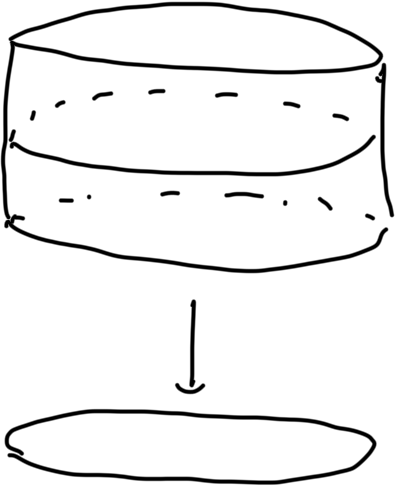
\includegraphics[width=0.2\textwidth]{cylinder.png}
    \qquad
    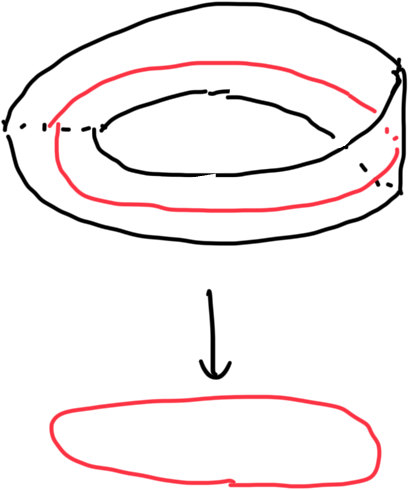
\includegraphics[width=0.2\textwidth]{mobius.png}
  \]
    \caption{A cylinder and a M\"obius strip.}
    \label{fig:cyl-mob}
\end{figure}

\begin{example}
A cylinder $S^1\times [-1,1]$ is a fiber bundle over $S^1$ with fiber $[-1,1]$.
\end{example}

\begin{example}
A M\"obius strip is a fiber bundle over $S^1$, where the fiber is the segment $[-1,1]$.
\end{example}

\noindent See Fig.~\ref{fig:cyl-mob} for my terrible drawings.


A cylinder and a M\"obius strip are inequivalent,
although the fiber and the base of both cases are the same.
One way to see this is to note that the boundary of 
the cylinder is $S^1\sqcup S^1$, while the boundary of the M\"obius strip is $S^1$.
Developing more general methods to distinguish different fiber bundles
with the same fiber and the same base is one of the goals
of the study of fiber bundles.

\subsection{Principal $G$-bundles}
\subsubsection{Generalities}
\begin{proposition}
  \label{prop:free-quotient}
Suppose $G$ acts on a manifold $M$.
We further suppose that this action is free,
i.e.~for each $m\in M$ the only $g\in G$ such that $mg=m$ is $g=e$.
Then the projection $p: M\to M/G$ is a fiber bundle with fiber $G$.
In other words, we have a fiber bundle $G\to M\to M/G$.
\end{proposition}

In this description it can be said that we are giving the total space $M$ 
more importance than the base $M/G$.
If we consider the base $B=M/G$, as the primary object, we get to the following viewpoint:

\begin{definition}
  \label{def:principal-bundle}
  A fiber bundle $p: P\to B$ with fiber $G$ is called a principal $G$-bundle
  if $P$ is equipped with an action of $G$ from the right, such that 
  for each $b\in B$ we have $U\subset B$ so that we have
  the following identification compatible with the $G$ action:
  \begin{equation}
  \begin{array}{ccc}
    p^{-1}(U) & \simeq & U\times G \\
    \downarrow & & \downarrow \\
    U & = & U
  \end{array} .
  \end{equation}
\end{definition}


Now, the total space $P$ is built 
as before by gluing $U_i\times G$ and $U_j\times G$ over $U:=U_i \cap U_j$ as 
\begin{equation}
  \begin{array}{cccccccc}
    U_i \times G &\supset& U\times G & \xrightarrow{f_{ij}} & 
    U\times G & \subset & U_j\times G \\
    \downarrow & & \downarrow & & \downarrow & & \downarrow \\
    U_i & \supset & U & = & U & \subset & U_j
  \end{array}
\end{equation}
where $f_{ij}$ has to be compatible with the right action of $G$.
Let us make $f_{ij}$ more explicit.

For this we need to use the following tautological lemma:
\begin{lemma}
A map $f:G\to G$ compatible with the right $G$ action is given by 
a left multiplication by an element $g\in G$, $f(h)=gh$.
\end{lemma}
Indeed, we need to have $f(h_1 h_2) = f(h_1) h_2$.
Therefore $f(h)=f(eh)=f(e)h$. Defining $g:=f(e)$, we have $f(h)=gh$.
This completes the proof.

Using this lemma at each point $b\in U$,
we find that  $f_{ij}: U\times G\to U\times G$ is given explicitly by
\begin{equation}
  f_{ij}: (b,g) \mapsto (b, g_{ij}(b) g)
  \label{eq:principal-bundle-transition-function}
\end{equation}
by a function $g_{ij}: U\to G$.

When is a principal $G$-bundle $P\to B$ equivalent to the trivial bundle $B\times G \to B$?
By definition this means that there is a bijective map $h: P\to B\times G$
compatible with the projections and the $G$ action from the right.
On each patch $U_i$, $h$ is given by $f'_i: p^{-1}(U_i)\to U_i\times G$
compatible with the $G$ action and the projection.
Using the above lemma again,
it is determined by a map $g'_i: U_i\to G$ via $f'_i(b,g)=(b,g'_i(b)g)$.
Furthermore, these maps $g'_i$ must be compatible with the patching procedure, i.e.~the following diagram must commute:
\begin{equation}
\vcenter{\xymatrix{
  G \ar[r]^{g_{ij}} \ar[d]_{g'_i} & G \ar[d]^{g'_j} \\
  G \ar[r]^{\text{id}} & G 
}},
\end{equation}
i.e.~$g_{ij} = (g'_j)^{-1} g'_i$.
Summarizing, we found: 
\begin{proposition}
  A principal $G$-bundle $P\to B$
  given in terms of \eqref{eq:principal-bundle-transition-function}
  is equivalent to the trivial principal $G$-bundle $B\times G \to B$
  if and only if there are maps $g_i: U_i\to G$ such that $g_{ij} = (g_j)^{-1} g_i$.
\end{proposition}

\subsubsection{Examples}

Now many of the examples we saw in Sec.~\ref{sec:quotient} can be rephrased as principal bundles.
In particular, Proposition \eqref{prop:sphere-proj} means the following:
\begin{example}
  \label{ex:RPn}
$S^n\to \RP^n$ is a principal $O(1)=\bZ_2$-bundle.
\end{example}

\begin{example}
  \label{ex:CPn}
$S^{2n+1}\to \CP^n$ is a principal $U(1)=S^1$-bundle.
\end{example}

\begin{example}
  \label{ex:HPn}
  $S^{4n+3}\to \HP^n$ is a principal $Sp(1)=SU(2)=S^3$-bundle.
\end{example}

Furthermore, we saw that $\RP^1=S^0$, $\CP^1=S^2$, $\HP^1=S^3$ 
in \eqref{eq:KP1}. 
This means that we have the following fiber bundles:
\begin{itemize}
  \item $\bR^2\supset S^1\to \RP^1=S^1$  is an $S^0$ bundle,
  \item $\bC^2\supset S^3\to \CP^1=S^2$ is an $S^1$ bundle,
  \item $\bH^2\supset S^7\to \HP^1=S^4$ is an $S^3$ bundle.
\end{itemize}

These are known as Hopf fibrations.
These bundles are nontrivial
and are different from a product.
For example, in the second case,
the total space is $S^3$,
which is different from $S^2\times S^1$,
the total space of a trivial $S^1$ fiber bundle over $S^2$.
(Note that we haven't actually learned how to distinguish
$S^3$ and $S^1\times S^2$.
This we will do later.)

%We have a few comments.
\begin{remark}
The first example is a 2:1 map,
already drawn in Fig.~\ref{fig:cyl-mob} 
as a map from the boundary $S^1$ of the M\"obius strip to the base $S^1$.
\end{remark}
\begin{remark}
The second example can be given a different description. 
Regard $S^3$ as parameterizing norm-one states
in a qubit:
\begin{equation}
  \ket{\psi}=\begin{pmatrix}u \\v \end{pmatrix},
  \qquad (|u|^2+|v|^2=1).
\end{equation}
Now form the expectation values of Pauli matrices:
\begin{align}
  x &:= \bra{\psi} \sigma_X \ket{\psi} = \bar u v + \bar v u, \\
  y &:= \bra{\psi} \sigma_Y \ket{\psi} = -i\bar u v +i \bar v u, \\
  z &:= \bra{\psi} \sigma_Z \ket{\psi} = |u|^2 - |v|^2.
\end{align}
It is straightforward to check that $x^2+y^2+z^2=1$.
Therefore the map \begin{equation}
(u,v)\mapsto (x,y,z)
\label{eq:uvXYZ}
\end{equation} defines a map \begin{equation}
  S^3\to S^2.
\end{equation}
That the fiber of this map is an $S^1$ is clear from the fact
that the expectation values are invariant under the change
$\ket{\psi}\mapsto c\ket{\psi}$ where $|c|=1$.
The sphere $S^2$ parameterized by $(x,y,z)$ is often referred to as the Bloch sphere of the qubit.\footnote{%
The history behind this terminology is quite interesting.
It originates in \cite{ACGT}, a paper about quantum optics,
where the authors refer to a work of Felix Bloch on nuclear magnetic resonance \cite{Bloch}, 
although this particular paper by Bloch does not study at all the Bloch sphere as we know it.
This was then adopted by the quantum information community,
which then became a standard terminology more generally, due to the increasing popularity of qubits. 
(I used \url{https://physics.stackexchange.com/questions/636913/} as a source.)
}
We can also give a more explicit parameterization of the map above:
\begin{equation}
  \label{eq:Hopf-explicit}
(\cos(\theta/2)  e^{i \psi},
\sin(\theta/2) e^{i(\phi+\psi)} )
\mapsto  (\sin\theta\cos\phi,\sin\theta\sin\phi,\cos\theta).
\end{equation}
This shows that the fiber above a point on $S^2$ is parameterized by $\psi$.

We can stereographically project points on $S^3$ to $\bR^3$ via \begin{equation}
(a,b,c,d) \mapsto \frac{1}{1-a}(b,c,d),
\end{equation} see Fig.~\ref{fig:stereo}.
Using this, we can draw the fibers of each point on $S^2$ as circles within $\bR^3$.
In Fig.~\ref{fig:hopf-fibers}, I drew the fibers of $(\cos 2\pi k/8, \sin 2\pi k/8, 0)$ for $k=0,1,\ldots,7$ in this manner.
\begin{figure}[h]
\centering   
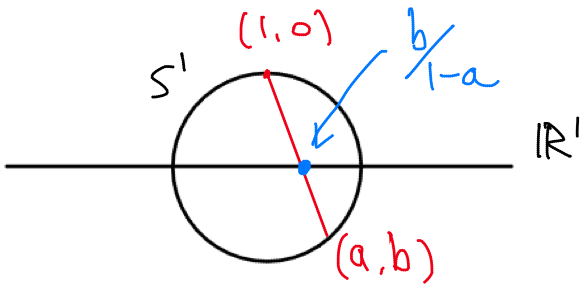
\includegraphics[width=0.3\textwidth]{stereo.png}
  \caption{Stereographical projection from $S^3$ to $\bR^3$}
  \label{fig:stereo}
\end{figure}
\begin{figure}[h]
\centering   
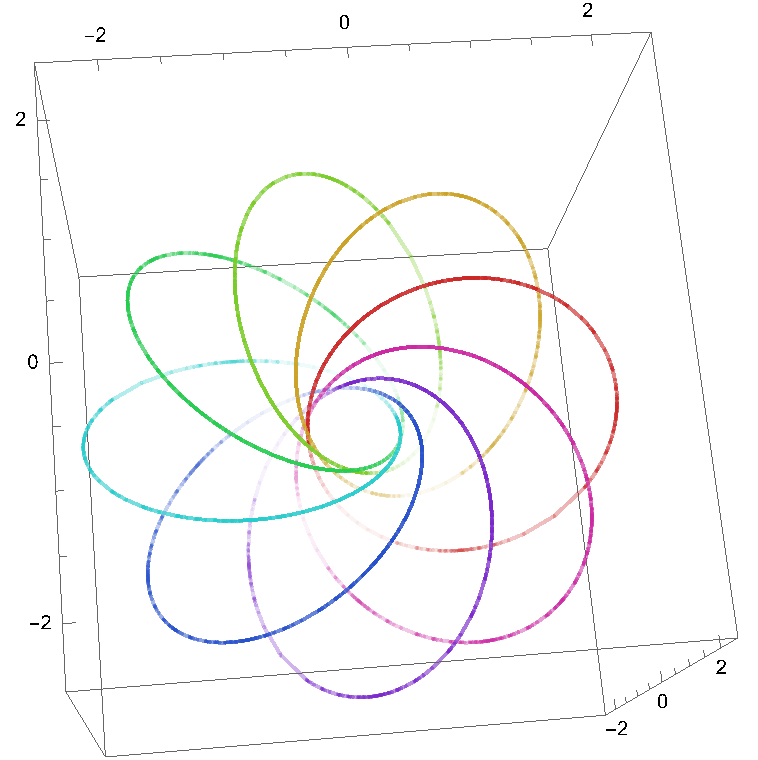
\includegraphics[width=0.5\textwidth]{hopf-fibers.png}
  \caption{Fibers of the Hopf fibration, drawn after a stereographic projection.}
  \label{fig:hopf-fibers}
\end{figure}
\end{remark}


Note that all the three fibrations above have the form
$S^n \to S^m \to S^{m-n}$.
One wonders if there are other examples of this form.
Actually we have:
\begin{fact}
These three Hopf fibrations, together with a final one
$S^7\to S^{15}\to S^8$
 exhaust 
such fibrations $S^n\to S^m\to S^{m-n}$.
\end{fact}
The last one, related to octonions, is not a principal fiber bundle, since $S^7$ is not a group.

We can also use the fact that Hopf fibrations are nontrivial to show that
the fibrations given in Examples \ref{ex:RPn}, \ref{ex:CPn}, \ref{ex:HPn} 
are all nontrivial.
Let us show this in the case of $\RP^n$. For this, we consider the following commutative diagram:
\begin{equation}
\begin{array}{ccccc}
  \bZ_2 &\to& S^n &\to& \RP^{n}  \\
   \rotatebox{90}{$=$} & & \cup & & \cup \\
    \bZ_2 &\to& S^1 &\to& \RP^1
\end{array}.
\end{equation}
Here, $S^1\subset S^n$ is obtained by restricting most of the coordinates to be zero.
We already saw that the second line is a nontrivial fibration.
As the first line contains the second line, the first line is also nontrivial.
Summarizing, we have: 
\begin{proposition}
  \label{prop:nontriviality-projective-fibration}
  The fibrations $\bZ_2\to S^n\to \RP^n$,
  $S^1\to S^{2n+1}\to \CP^n$,
  $S^3\to S^{4n+3}\to \HP^n$
  are all nontrivial.
\end{proposition}

The homogeneous spaces, introduced in Definition~\ref{def:homogeneous-space}
with many examples below it,
also give rise to principal bundles.
\begin{proposition}
  $G$ is a principal $H$-bundle over $G/H$, i.e.~we have a fiber bundle $H\to G\to G/H$.
\end{proposition}

Let us give an example not directly treated in Section~\ref{sec:homogeneous}.
Consider $g\in SU(2)$ acting on $\bC^2$.
Note that $2\times 2$ traceless Hermitean matrices are paramaterized by $\bR^3$,
by $x\sigma_x+y\sigma_y+z\sigma_z$.
We let $g\in SU(2)$ acts on this space via \begin{equation}
R_g: (x,y,z) \mapsto (x',y',z')  \label{eq:Rg1}
\end{equation} where \begin{equation}
g(x\sigma_x+y\sigma_y+z\sigma_z)g^\dagger = x'\sigma_x+y'\sigma_y+z'\sigma_z.
\label{eq:Rg2}
\end{equation}

An function $V:\bR^3\to \bR$ invariant under this $SU(2)$ action 
has the form $V(x,y,z)=f(r)$ where $r^2={x^2+y^2+z^2}$.
Suppose $f(r)$ has a minimum at $r_0>0$.
The space of the potential minimum is $x^2+y^2+z^2=r_0^2$, which is a sphere $S^2$.
Take $m_0=(0,0,r_0)$, corresponding to $r_0 \sigma_z$.
The elements of $SU(2)\simeq S^3$ fixing this point have the form $e^{i\theta \sigma_z}$ for some $\theta$,
and is isomorphic to $U(1)\simeq S^1$.
In this way we again found \begin{equation}
  S^1 \to S^3 \to S^2.
\end{equation}
This symmetry breaking pattern was first introduced by Georgi and Glashow in the context of the electroweak theory \cite{Georgi:1972cj}.
Although it does not match the experimental results,
it still serves as a model simpler than the reality (the Standard Model),
where we can practice our techniques. 
It will play an important role in our analysis of monopoles later, too.

Note that we have defined a map $SU(2)\to SO(3)$ by $g\mapsto R_g$ where $R_g$ was given in \eqref{eq:Rg1} and \eqref{eq:Rg2}.
This is a homomorphism, and the kernel is $\{\pm 1\}$.
In other words we have found:
\begin{example}
  There is a fiber bundle $
    \{\pm 1\} \to SU(2) \to SO(3). 
  $
\end{example}
Recalling that $SU(2)\simeq S^3$, we also see that 
\begin{proposition}
$SO(3)\simeq \RP^3$.  
\end{proposition}

Note that this is simply an example of the fibration $\bZ_2\to S^n\to \RP^n$
for $n=3$,
which therefore is nontrivial, as we already saw in Proposition~\ref{prop:nontriviality-projective-fibration}.

\subsection{Vector bundles}

Another large class of bundles is given by the vector bundles,
where the fiber is a vector space.

\begin{definition}
  Pick the field of scalars $\bK$ to be either $\bR$, $\bC$ or $\bH$.
  A vector bundle is a fiber bundle $E\to B$ with fiber $V$,
  where $V$ is a vector space, such that two local trivializations over $U_i \subset B$
  and $U_j\subset B$ are related in the following manner on the overlap $U:=U_i\cap U_j$:
  \begin{equation}
  \begin{array}{cccccccc}
    U_i \times V &\supset& U \times V & \xrightarrow{f } & 
    U \times V & \subset & U_j\times V \\
    \downarrow & & \downarrow & & \downarrow & & \downarrow \\
    U_i & \supset & U  & = & U  & \subset & U_j
  \end{array}
  \end{equation}
  where $f $ is given by \begin{equation}
    f : (b,v) \mapsto (b, g (b) v)
    \label{eq:vec-bundle-transition-functions}
  \end{equation} where $g (b): V\to V$ is a linear map smoothly depending on $b\in U$.
  The dimension of $V$ is called the rank of the vector bundle.
\end{definition}
$\bR$-vector bundles, $\bC$-vector bundles, and $\bH$-vector bundles
are also called real, complex, and quaternionic vector bundles, respectively.

In physics it is also common to have an inner product on the fibers $V$ of a vector bundle,
so that the transition functions $g (b)$ are not just linear maps
but in $O(n)$, $U(n)$, or $Sp(n)$, respectively.
We will come back to this point later.


\begin{definition}
  A section of a vector bundle $p:E\to B$ is a map $\psi: B\to E$ such that $p\circ \psi $ is the identity map on $B$.
\end{definition}
More informally, $\psi(b)$ for $b\in B$ takes values in the fiber $V$ over $b$.
Sections of vector bundles appear in physics usually in one of the two ways:
\begin{itemize}
  \item As fields, where the base space $B$ is spacetime and 
  the fiber $V$ is the possible values the fields can take.
  This appears ubiquitously in hep-th, in the gauge theory setting.
  The metric tensor in general relativity is also a section of a vector bundle.
  \item As wavefunctions of a quantum mechanical system, 
  where the system can be separated 
  into the degrees of freedom along the base space $B$
  and additional degrees of freedom parameterized by the fiber $V$ 
  which is the Hilbert space of a quantum subsystem.
  This arise, for example, in the Born-Oppenheimer approximation,
  where $B$ is for the slow motion of some degrees of freedom (such as the position of the nuclei) and 
  $V$ is for the fast motion of other degrees of freedom (such as electrons).
  It can also arise in the study of crystalline materials,
  where $B$ is the Brillouin zone and $V$ is the spaces of quantum states at fixed wave number.
\end{itemize}

\begin{definition}
A vector bundle whose fiber is one dimensional over $\bK$ is called a 
$\bK$-line bundle.
Here $\bK$ is either $\bR$, $\bC$ or $\bH$.
\end{definition}
Most often, a line bundle refers to a complex line bundle, i.e.~a vector bundle
whose fiber is a one-dimenisonal complex vector space.\footnote{%
I think mathematicians are crazy in that they call the space of complex numbers a `line'.
}

When we have two vector spaces $V$ and $W$,
we can form the direct sum $V\oplus W$ or the tensor product $V\otimes W$.
These operations can be lifted to vector bundles,
by performing them fiberwise.
\begin{definition}
  Given two vector bundles $E\to B$ and $E'\to B$ with fibers $V$ and $W$,
  we can form the direct sum $E\oplus E'$ over $B$ with fiber $V\oplus W$,
  or the tensor product bundle $E\otimes E'$ over $B$ with fiber $V\otimes W$.  
\end{definition}

Given a vector space $V$, the space of linear functions $V\to \bK$ is denoted by $V^*$
and is also a  vector space.
Doing this fiberwise, we have:
\begin{definition}
  Given a vector bundle $E\to B$ with fiber $V$,
  we can form the dual bundle $E^*\to B$ whose fiber is $V^*$.
\end{definition}
Similarly, for a complex vector bundle, we can do:
\begin{definition}
  Given a complex vector bundle $E\to B$ with fiber $V$,
  we can form the complex conjugate bundle $\bar E\to B$ whose fiber is $\bar V$.
\end{definition}


Another interesting operation one can do is the following:
Let $V$ be a complex vector space with a Hermitian inner product.
Let $\mathrm{Herm}(V)$ be the space of Hermitian operators on $V$,
which is a real vector space.
\begin{definition}
  Given a complex vector bundle $E\to B$ with fiber $V$,
  we can form the bundle of Hermitian operators $\mathrm{Herm}(E)\to B$ with fiber $\mathrm{Herm}(V)$.
\end{definition}
This is the operation which, given a family of Hilbert spaces parameterized over 
a parameter space $B$,
produces the family of spaces of observables acting on each Hilbert space, over the same parameter space $B$.

A somewhat different operation one can perform fiberwise 
is to take the unit sphere $Sph(V)=S^{kn-1} \subset V$ at each fiber, where $n$ is the dimension of $V$
and $k=1,2,4$ for $\bK=\bR,\bC,\bH$.
\begin{definition}
  Given a vector bundle $E\to B$ with fiber $V$,
  we can form the sphere bundle $Sph(E)\to B$ whose fiber is $Sph(V)$.
\end{definition}

We can also consider taking a vector subspace $V_2\subset V_1$ at each fiber:
\begin{definition}
A subbundle of a vector bundle $E_1\to B$ with fiber $V_1$ is 
a vector bundle $E_2\to B$ with fiber $V_2$ such that on each local trivialization 
we have 
\begin{equation}
  \begin{array}{cccccccc}
    (p_2)^{-1}(B) &\simeq & U\times V_2 & \subset  & U\times V_1 &\simeq & (p_1)^{-1}(B) \\ 
    \downarrow & & \downarrow & & \downarrow & & \downarrow \\
    U & = & U & = & U & = & U
  \end{array}
  \end{equation}
\end{definition}

Let us consider a basic but interesting example.
Consider the unit sphere $S^2$, parameterized by $(x,y,z)$ with $x^2+y^2+z^2=1$.
We consider a trivial vector bundle $S^2\times \cH$ over $S^2$,
where $\cH=\bC^2$ is a qubit.
Let us consider the Hamiltonian \begin{equation}
  H := -(x\sigma_x +y \sigma_y + z\sigma_z)
  \label{eq:S2Ham}
\end{equation} parameterized over $S^2$.
As $H^2=1$, the eigenvalues of $H$ are $\pm 1$.
Let $V(x,y,z) \subset \cH$ be the eigenspace of the lowest energy, i.e.~the $-1$ eigenspace.
This determines a subbundle $E \to S^2 $ of the trivial bundle $S^2\times \cH$,
where the fiber at $(x,y,z)$ is $V(x,y,z)$.
This is a complex line bundle.

To have a more explicit description of this bundle,
let us recall the map \eqref{eq:uvXYZ} from $S^3$ to $S^2$;
we write $(x,y,z)$ in terms of $(u,v)$.
We can easily check that 
\begin{equation}
H \begin{pmatrix}
u\\ v
\end{pmatrix}
=
- \begin{pmatrix}
|u|^2-|v|^2 & 2\bar v u \\
2 \bar u v & -|u|^2+|v|^2
\end{pmatrix}
\begin{pmatrix}
  u\\ v
  \end{pmatrix}
=
-\begin{pmatrix}
  u\\ v
\end{pmatrix}.
\end{equation}
We have shown that 
\begin{equation}
  V(x,y,z)= \{ c\begin{pmatrix}
    u\\ v
  \end{pmatrix}  \mid c\in \bC \} \subset \cH.
\end{equation} 
We can now take the unit sphere bundle $Sph(E)\to S^2$.
This simply sends $(u,v)$ with $|u|^2+|v|^2=1$ to $(x,y,z)$ via \eqref{eq:uvXYZ},
so this is the Hopf fibration $S^1\to S^3\to S^2$.
Summarizing:
\begin{example}
  \label{ex:S2parameterized}
  The unit sphere bundle 
  of the complex line bundle over $S^2$,
  obtained by taking the lowest energy states 
  of the Hamiltonian \eqref{eq:S2Ham},
  is the Hopf fibration $S^1\to S^3\to S^2$.
\end{example}

\subsection{Relating vector bundles and principal $G$-bundles}

We described the transition functions of a vector bundle in Eq.~\eqref{eq:vec-bundle-transition-functions}.
On a completely general complex vector bundle $E\to B$,
the transition functions $g (b)$ are in $GL(n,\bC)$,
where $n$ is the rank of the vector bundle, i.e.~the dimension of the fiber. 
But we often consider the situation where the fibers of the vector bundle are equipped with a Hermitian inner product.
In such a case, the transition functions are in $U(n)$.
Then we can consider a principal $U(n)$-bundle $P\to B$ associated to the vector bundle, 
defined via \eqref{eq:principal-bundle-transition-function}.
The fiber is now $U(n)$ instead of $\bC^n$.

In high-energy physics we often encounter the situation where $g (b)$ is in a subgroup $G$ of $U(n)$;
then we can consider the principal $G$-bundle associated to the vector bundle in the same way.
The fiber is now $G$ instead of $\bC^n$.

\begin{definition}
  A $\bK$-vector bundle whose transition functions $g(b)$ are in a subgroup $G$ of $GL(n,\bK)$
  is called to have the structure group $G$.
  The principal $G$-bundle given by the same transition functions are called 
  the  principal $G$-bundle associated to the vector bundle.
\end{definition}

There is an inverse operation to this.
Take a principal $G$-bundle over $B$
with the transition function over $U:=U_i\cap U_j$ given by
a map $g: U\to G$ as described in \eqref{eq:principal-bundle-transition-function}.
Pick a linear action $\rho: G \curvearrowright V$ of $G$ on a vector space $V$.
Then we can form a vector bundle over $B$ with fiber $V$
by declaring that its transition functions 
between $U_i\times V$ and $U_j\times V$
are given by $\rho(g)$, i.e.~we have
\begin{equation}
  \begin{array}{cccccccc}
    U_i \times V &\supset& U \times V & \xrightarrow{f } & 
    U \times V & \subset & U_j\times V \\
    \downarrow & & \downarrow & & \downarrow & & \downarrow \\
    U_i & \supset & U  & = & U  & \subset & U_j
  \end{array}
\end{equation}
where $f $ is given by \begin{equation}
   f : (b,v) \mapsto (b, \rho(g (b)) v).
\end{equation}


\begin{definition}
  The vector bundle $V\to E\to B$ constructed as above is called 
  an associated vector bundle to the principal $G$-bundle $G\to P\to B$,
  determined by the representation $\rho$.
  We call $G$ the structure group of $E\to B$.
\end{definition}

As an example, take a principal $U(1)$ bundle $U(1)\to E\to B$.
\begin{equation}
  \begin{array}{cccccccc}
    U_i \times U(1) &\supset& U \times U(1) & \xrightarrow{f } & 
    U \times U(1) & \subset & U_j\times U(1) \\
    \downarrow & & \downarrow & & \downarrow & & \downarrow \\
    U_i & \supset & U  & = & U  & \subset & U_j
  \end{array}
\end{equation}
where $f $ is given by \begin{equation}
   f : (b,h) \mapsto (b, g(b)h)
   \label{eq:U1-transition-function}
\end{equation} where $b\in B$, $h\in U(1)$ (i.e.~$|h|=1$) and $g: U\to U(1)$.
Take the standard representation of $U(1)$ on $\bC$ given by multiplication,
i.e. the one where $g\in U(1)$ acts on $z\in \bC$ by $gz$.
Then the associated vector bundle $\bC\to E'\to B$ has the structure 
\begin{equation}
  \begin{array}{cccccccc}
    U_i \times \bC &\supset& U \times \bC & \xrightarrow{f' } & 
    U \times \bC & \subset & U_j\times \bC \\
    \downarrow & & \downarrow & & \downarrow & & \downarrow \\
    U_i & \supset & U  & = & U  & \subset & U_j
  \end{array}
\end{equation}
where $f $ is given by \begin{equation}
   f' : (b,z) \mapsto (b, g(b)z)
   \label{eq:line-bundle-transition-function}
\end{equation} where $z\in \bC$.
It is easy to see that $E\to B$ is the unit sphere bundle of $E'\to B$.
Summarizing, we found:
\begin{proposition}
  Given a principal $U(1)$-bundle $U(1)\to E\to B$,
  consider the associated vector bundle $\bC\to E'\to B$
  coming from the standard representation $U(1)\curvearrowright \bC$.
  Then $E\to B$ is the unit sphere bundle of $E'\to B$.
\end{proposition}

We saw in Example~\ref{ex:S2parameterized} that the unit sphere bundle
of the complex line bundle of the lowest energy states of the Hamiltonian \eqref{eq:S2Ham}
over $S^2$ is the Hopf fibration $S^1\to S^3\to S^2$.
Therefore, conversely, the associated line bundle
to the Hopf fibration $S^1\to S^3\to S^2$ 
in the standard representation $U(1)\curvearrowright \bC$
is the complex line bundle of the lowest energy states of the Hamiltonian \eqref{eq:S2Ham}.

An alternative construction of the associated vector bundle 
without using patches is as follows. 
\begin{proposition}
  Given a principal $G$-bundle $G\to P\to B$ and a representation $\rho: G\curvearrowright V$,
  the associated vector bundle $V\to E\to B$ is given by
  $E= (P \times V)/G$,
  where the action of $G$ on $P\times V$ is given by $g(p,v)=(pg^{-1},\rho(g)v)$.
\end{proposition}
The proof is straightforward and is left as an exercise.

\subsection{Tangent and cotangent bundles}

\subsubsection{Definitions}
So far we considered vector bundles as an additional structure on a given base $B$.
There are also vector bundles canonically associated to a manifold $M$.

Take two patches $U$ and $U'$ on a manifold
with a nontrivial overlap $U\cap U'$.
and with $f:U\to \bR^n$ and $f':U'\to \bR^n$ respectively.
For a point $p\in U\cap U'$ in the overlap,
let $f(p)=(x^1,\ldots,x^n)$ and $f'(p)=(x'{}^1,\ldots,x'{}^n)$.
Here we placed the indices on the superscripts, following the convention in general relativity.
We now consider $U\times \bR^n$,
where the basis vectors for the $\bR^n$ factor
are the symbols
\begin{equation}
\frac{\partial}{\partial x^1},\ldots,\frac{\partial}{\partial x^n}.
\end{equation}
Similarly, we consider $U'\times \bR^n$
where the $\bR^n$ factor has the basis vectors
\begin{equation}
\frac{\partial}{\partial x'{}^1},\ldots,\frac{\partial}{\partial x'{}^n}.
\end{equation}
We let these two vasis vectors to be related as usual:
\begin{equation}
\frac{\partial}{\partial x'{}^i} = \sum_{j}\frac{\partial x^j}{\partial x'{}^i} \frac{\partial}{\partial x^j}.
\label{eq:contravariant}
\end{equation}
In other words, on the overlap $U\cap U'$,
the transition function $U\times \bR^n \to U'\times \bR^n$ is given by 
\begin{equation}
  (p,\sum_i c^i\frac{\partial}{\partial x_i} )
  \mapsto 
  (p, \sum_{i,j} c^i \frac{\partial x^j}{\partial x'{}^i} \frac{\partial}{\partial x^j}).
\end{equation}

\begin{definition}
For a smooth manifold $M$ of dimension $n$,
the real $n$-dimensional bundle constructed as above is called the tangent bundle and is denoted by $TM$.
\end{definition}

\begin{definition}
The dual bundle of the tangent bundle is called the cotangent bundle and is denoted by $T^*M$.
\end{definition}
More explicitly, consider patches $U\subset M$
and $U'\subset M$ as above,
with $f(p)=(x^1,\ldots,x^n)\in \bR^n$
and $f'(p)=(x'{}^1,\ldots,x'{}^n)\in \bR^n$, respectively.
Then the cotangent bundle $T^*M$ has the local trivialization
$U\times \bR^n$  and $U'\times \bR^n$
with the basis vectors on the $\bR^n$ part
given by $dx^i$ and $dx'{}^i$, respectively.
These two sets of basis vectors are related by 
\begin{equation}
  dx'{}^i = \sum_j \frac{\partial x'{}^i}{\partial x^j} dx^j.
  \label{eq:covariant},
\end{equation}
compare Eq.~\ref{eq:contravariant}.


Consider a function $\phi:M \to \bR$ on an $M$-dimensional manifold $M$.
Where does the derivative $\nabla f$ of $\phi$ live?
Take a local patch $f:U\to \underline{U}\subset \bR^n$ with $U\subset M$,
with coordinates $(x^1,\ldots,x^n)$.
Consider the object \begin{equation}
d\phi := \sum_i \frac{\partial \phi}{\partial x^i} dx^i.
\end{equation}
Using the relation \eqref{eq:covariant},
we can check that $df: U\to U\times \bR^n$ 
on each patch $U$ consistently defines a section of the cotangent bundle 
$d\phi: M\to T^*M$.
\begin{definition}
  \label{def:exterior-derivative}
  $d\phi$ defined above is called the exterior derivative of $\phi$,
  and is a section of $T^*M$.
\end{definition}

We can easily check the following: \begin{proposition}
$d(fg)=(df)g+ f(dg)$.
\end{proposition}

\subsubsection{The metric}

So far we have not introduced a metric. Let us do so now:

\begin{definition}
A Riemannian metric on a manifold $M$
is an additional structure on the tangent bundle $TM$
which gives a smoothly-varying inner product 
on each fiber.
\end{definition}

\paragraph{Unit sphere bundle:}
With a metric, we can consider the unit sphere bundle $Sph(TM)$.

\begin{example}
Let $M=S^2$ and consider its tangent bundle $TS^2$.
This is a real 2-dimensional bundle.
Give a standard round metric on $S^2$,
and take the unit sphere bundle $Sph(TS^2)$ of its tangent bundle.
This is an $S^1$ bundle over $S^2$.
\end{example}
We have already encountered two $S^1$ bundles over $S^2$,
namely the trivial product and the Hopf fibration.
Is $Sph(TS^2)$ one of these two?
The answer is no.
We are going to develop general methods to answer such questions later,
but here is a special argument applicable to this particular case.
\begin{example}
$Sph(TS^2) \simeq SO(3)$.
\end{example}

\begin{proof}
To see this, note that $SO(3)$ naturally acts on $TS^2$ by rotation;
if you are unsure, realize $TS^2$ as a subspace of $(\vec v,\vec w) \bR^3\times \bR^3$
with the constraint $\vec v\cdot \vec v=1$, $\vec w\cdot \vec v=0$.
Clearly $SO(3)$ acts on it by simultaneous rotation of $\vec v$ and $\vec w$.

Now pick a point $\vec v_0 \in S^2$ and a point on the fiber over it with unit length, 
i.e.~ a point $\vec w_0$ such that $\vec w_0\cdot \vec w_0=1$ and $\vec w_0\cdot \vec v_0 =0$.
What is the orbit of this point $(\vec v_0,\vec w_0)\in TS^2$?

As we saw in Sec.~\ref{sec:homogeneous}, the orbit is of the form $SO(3)/H$, where $H$ is the subgroup fixing this point.
Now, $\vec v_0$ is fixed by $SO(2)\subset SO(3)$, but this $SO(2)$ rotates $\vec w_0$.
Therefore $H=\{e\}$, and the orbit is $SO(3)$ itself.
Clearly this orbit is $Sph(TS^2)$, and we are done.
\end{proof}

Note that, at this point, we learned of the existence of three different $S^1$ bundles over $S^2$:
\begin{itemize}
\item The trivial one, $S^1\to S^1\times S^2\to S^2$,
\item The Hopf bundle, $S^1\to S^3\to S^2$,
\item the bundle $S^1\to Sph(TS^2)\to S^2$.
\end{itemize}

\paragraph{Reduction of the structure group to $O(n)$ or $O(n-1,1)$:}
We now consider a different use of the metric.
With a Riemannian metric, we can form an orthogonal basis of the tangent space at each point.
Take $U\times \bR^n$ with the basis vectors $\partial/\partial x^i$ as before.
We pick an orthonormal basis \begin{equation}
  e_a = \sum e_a^i \frac{\partial}{\partial x^i},
  \qquad (a=1,\ldots,n)
\end{equation} with respect to the inner product on the tangent space given by the metric,
where $e_a^i$ is an $n\times n$ matrix depending on $p\in U$.
In other words, we have \begin{equation}
\langle e_a, e_b \rangle = \delta_{ab}.
\end{equation}
In general relativity $e_a^i$ are known as tetrads or vierbeins 
in four dimensions, and fielbeins in general dimensions.
On $U'\times \bR^n$ we pick a similar orthonormal basis $e'_a$
given by \begin{equation}
  e_a' = \sum e_a'{}^i \frac{\partial}{\partial x'{}^i},
  \qquad (a=1,\ldots,n)
\end{equation}
and we have the following relation on the overlap $p\in U\cap U'$:  \begin{equation}
  e_a'{}^i = \sum_b M_a^b e_b
\end{equation} 
where $M_a^b$ is an orthogonal matrix depending on $p$,
i.e.~$M$ is a map from $U\cap U'$ to $O(n)$.
Then the tangent bundle has the structure group $O(n)$.

In physics we also often encounter the situation
when the tangent bundle is equipped with a Lorentzian inner product.
In such cases the orthonormal basis $e_a$ above satisfies
\begin{equation}
  \langle e_a, e_b \rangle = \eta_{ab},\qquad
  \text{where}
  \quad
  \eta_{ab} = \mathrm{diag}(1,\ldots,1,-1).
\end{equation}
Then the matrix $M_a^b$ is in the Lorentz group $O(n-1,1)$,
which is the structure group of the tangent bundle.

Below, we will always consider the case when the tangent bundle is
equipped either with a Riemannian or a Lorentzian metric;
furthermore, we consider the Riemannian case unless otherwise mentioned.

\subsection{Orientation and spin structure}

We have seen so far that the tangent bundle $TM$ of a manifold $M$ of dimension $n$
is a real vector bundle with structure group $O(n)$.
In other words, it is built by patching the fiber over the intersection $U:=U_i\cap U_j$
with the following structure: 
\begin{equation}
  \begin{array}{cccccccc}
    U_i \times \bR^n  &\supset& U \times \bR^n  & \xrightarrow{f } & 
    U \times \bR^n  & \subset & U_j\times \bR^n  \\
    \downarrow & & \downarrow & & \downarrow & & \downarrow \\
    U_i & \supset & U  & = & U  & \subset & U_j
  \end{array}
\end{equation}
where $f $ has the form \begin{equation}
   f : (b,v) \mapsto (b, g(b) v), \qquad g: U\to O(n).
\end{equation} 

Recall that $O(n)$ has a subgroup $SO(n)$ consisting of the matrices with determinant 1,
and has the decomposition \begin{equation}
O(n) = SO(n) \sqcup SO(n)e
\end{equation} where $e$ is an element of determinant $-1$.
$SO(n)$ contains $n$-dimensional rotations and preserves the orientation of $\bR^n$.

\begin{definition}  
When $g:U\to O(n)$ above can be uniformly chosen to be in $SO(n)$
over any nonempty intersection $U=U_i\cap U_j$ of two patches,
the tangent bundle $TM$ is not just an $O(n)$-bundle but an $SO(n)$-bundle.
In such case we say that the manifold $M$ is orientable.
\end{definition}

On $\bR^3$ we have two orientations of basis vectors.
Similarly, when a manifold is orientable (and is connected),
there are actually two orientations of the manifold.

Let us move on to the spin structure,
which is necessary if we want to consider spinors on a manifold.
Let us start by considering the familiar case of three dimensions.
The rotations of $\bR^3$ form the group $SO(3)$.
The double cover of $SO(3)$ is the group $SU(2)$: 
\begin{equation}
  \{\pm1\}\to SU(2) \xrightarrow{\pi} SO(3).
\end{equation}
The wavefunction of a spin $1/2$ particle is in the standard two-dimensional representation of $SU(2)$.
But this is not a representation of $SO(3)$.
Famously, a $360^\circ$ rotation acts by $-1$ on the wavefunction of an electron;
a $360^\circ$ rotation is the identity of $SO(3)$.
Therefore this two-dimensional representation is not a representation of $SO(3)$.
This means that the data of $g_{ij}:U_{ij}\to SO(3)$ 
on the overlaps $U_{ij}=U_i\cap U_j$ of the tangent bundle $TM$ 
is not sufficient for us to consider electrons on the manifold.

For this, we need to lift the maps $g_{ij}$ to $SO(3)$ uniformly to $SU(2)$,
i.e.~find maps $g'_{ij}:U_{ij}\to SU(2)$
such that $\pi\circ g'_{ij}=g_{ij}$ 
so that $\{g'_{ij}\}$ determine a principal $SU(2)$-bundle $P\to M$.
A choice of such an principal $SU(2)$ bundle is known as the spin structure,
and then we can consider the associated complex two-dimensional vector bundle
$S\to M$ 
given by the standard representation of $SU(2)$, by the construction 
\begin{equation}
  \begin{array}{cccccccc}
    U_i \times \bC^2  &\supset& U \times \bC^2  & \xrightarrow{f' } & 
    U \times \bC^2  & \subset & U_j\times \bC^2  \\
    \downarrow & & \downarrow & & \downarrow & & \downarrow \\
    U_i & \supset & U  & = & U  & \subset & U_j
  \end{array}
\end{equation}
where $f $ has the form \begin{equation}
   f : (b,v) \mapsto (b, g'(b) v), \qquad g: U\to SU(2).
\end{equation} 
This $S$ is the spinor bundle,
and the wavefunction of an electron is a section of this bundle.

In three dimensions we have the following fact:
\begin{fact}
  Any oriented three-dimensional manifold has a spin structure.
\end{fact}
At the end of the lecture series, I hope that you will understand the outline 
of the proof of this fact.  

To discuss spin structures in other dimensions, we need some preparations.
\begin{fact}
  There are nontrivial double covers of $SO(n)$ for $n\ge 2$ of the form
  \begin{equation}
  \{\pm1\} \to \Spin(n) \to SO(n)
  \end{equation} and double covers of $SO(n-1,1)$ for $n\ge 3$ of the form
  \begin{equation}
  \{\pm1\} \to \Spin(n-1,1) \to SO(n-1,1).
  \end{equation}
\end{fact}

\begin{fact}
$Spin(2k)$ has two spinor representations, each with complex dimensions $2^k$.\\
$Spin(2k+1)$ has one spinor representation, which is of complex dimensions $2^k$.
\end{fact}
We will give their uniform explicit descriptions later.
For low dimensions we have the following alternative ways to describe them:
  \begin{itemize}
    \item $\Spin(2)\simeq U(1)$. Two spinor representations are the standard representation and its complex conjugate,
    \item $\Spin(3)\simeq SU(2)$. The spinor representation is the standard two-dimensional representation,
    \item $\Spin(4)\simeq SU(2)\times SU(2)$. Two spinor representations are the standard two-dimensional representations of the two factors,
    \item $\Spin(5)\simeq Sp(2)$. The spinor representation is the standard  representation of $Sp(2)$ on $\bH^2 \simeq \bC^4$,
    \item $\Spin(6)\simeq SU(4)$. Two spinor representations are the standard four-dimensional representation and its conjugate;
  \end{itemize}
We also have
  \begin{itemize}
    \item $\Spin(2,1)\simeq SL(2,\bR)$. The spinor representation is the standard two-dimensional representation (regarded as complex matrices),
    \item $\Spin(3,1)\simeq SL(2,\bC)$. Two spinor representations are the standard representation and its complex conjugate.
  \end{itemize}

\begin{fact}
$\CP^2$ is not spin, i.e.~does not have a spin structure.
\end{fact}
Therefore you cannot consider electrons on $\CP^2$, a four dimensional space.\footnote{%
Actually, this is true as long as we do not couple electrons to electromagnetism.
With electromagnetism, we can consider something called a spin-$c$ structure,
which exists on $\CP^2$. This will require a nonzero Maxwell field on $\CP^2$.
Therefore it is still true that electrons cannot exist on $\CP^2$
if the electromagnetic field is zero.
}

\if0
\subsection{Gauge fields and $G$-bundles}

We saw in Definition~\ref{def:exterior-derivative} that 
the exterior derivative of a function $\phi$ on a manifold $M$
naturally is a section of the cotangent bundle $T^*M$.

Let us consider instead a complex line bundle $\bC\to L\to M$
associated to a $U(1)$ bundle $U(1)\to P\to M$,
described explicitly in Eq.~\ref{eq:U1-transition-function} and Eq.~\ref{eq:line-bundle-transition-function}
on the overlap $U:=U_i\cap U_j$.
Take a section $\psi:M\to L$ of this line bundle.
We would like to take the derivative of this section consistently.

Let us take two local patches $U_1$ and $U_2$ with coordinates $x^a$ and $x'{}^a$ as before.
We take local trivializations $U_1\times \bC$ and $U_2\times \bC$ of $L\to M$,
with the identification given by \begin{equation}
(b,v)\mapsto (b, g(b)v) 
\end{equation} on the overlap $b\in U_1\cap U_2$, where $g: U_1\cap U_2\to U(1)$.
A section $\psi$ of $L\to M$ then gives two functions
$\psi_1: U_1\to \bC$ and $\psi_2: U_2\to \bC$ satisfying \begin{equation}
  \psi_2(b) = g(b) \psi_1(b). \label{eq:psi}
\end{equation}

Let us now consider \begin{equation}
  d\psi_1 = \sum_a \frac{\partial \psi_1}{\partial x^a} dx^a
\end{equation} on $U$ ; this is a local section of \begin{equation}
  U_1 \times (\bC \otimes \bR^n). \label{eq:der1}
\end{equation}
Similarly, we have
\begin{equation}
  d\psi_2 = \sum_a \frac{\partial \psi_2}{\partial x'{}^a} dx'{}^a
  \label{eq:dpsiprime}
\end{equation} on $U_2$, which is a local section of \begin{equation}
  U_2 \times (\bC \otimes \bR^n). \label{eq:der2}
\end{equation}
Here we relate the basis vectors $dx^a$ and $dx'{}^a$ on the overlap $U_1\cap U_2$
as before by \eqref{eq:covariant}, so that we have \begin{equation}
  d\psi_2= \sum_a \frac{\partial \psi_2}{\partial x^a} dx^a
\end{equation}
on the overlap.

In view of \eqref{eq:der1} and \eqref{eq:der2},
it seems reasonable to try to let the derivative of $\psi$ to be a section of $L\otimes T^*M$. 
Such a section corresponds to $\varpi_1: U_1\to \bC\times \bR^n$
and $\varpi_2: U_2\to \bC \otimes \bR^n$ related by \begin{equation}
  \varpi_2(b) = g(b) \varpi_1(b)
\end{equation} over the overlap $U_1\cap U_2$.

Plugging \eqref{eq:psi} in \eqref{dpsiprime}, we find instead \begin{equation}
d\psi_2 = d (g\psi_1) = (dg ) \psi_1 + g d\psi_1.
\end{equation} with an additional first term.
To remedy the situation,
we introduce local sections 
$A_1: U_1\to \bR^n$, $A_2:U_2\to \bR^n$ of the cotangent bundle on the patches,
given more explicitly by \begin{equation}
  A_1 = \sum_a (A_1)_a dx^a, \qquad A_2 = \sum_a (A_2)_{'a} dx'{}^a,
\end{equation} 
which we demand to be related by \begin{equation}
  A_2 = A_1 + g^{-1} dg.\label{eq:AA}
\end{equation}
We also define \begin{equation}
  D\psi_1 = d\psi_1 + \ii A_1 \psi_1, \qquad D\psi_2 = d\psi_2 + \ii A_2 \psi_2.
\end{equation}
We can check that $D\psi_1$ and $D\psi_2$ are related by \begin{equation}
  D\psi_2 = g D\psi_1,
\end{equation} as we wanted.

Consider the simpler case of $U=U_1=U_2$ with the same coordinate system,
where $x^a=x'{}^a$. 
Let us also write $g: U\to U(1)$ as $g(b)=e^{i\theta(b)}$.
Then we have \begin{equation}
A_2 
\end{equation}
\begin{definition}
connection = gauge field
\end{definition}

\begin{definition}
covariant derivative
\end{definition}

\begin{example}
Schr\"odinger eq.~in the presence of magnetic field
\end{example}

\begin{example}
$S^1\to S^3\to S^2$ as Dirac monopole
\end{example}

\begin{example}
affine connection, spin connection
\end{example}
 
\begin{example}
Gauge fields of the Standard Model
\end{example}

\begin{example}
Matter content of the Standard Model
\end{example}
\fi

\subsection{Bundles and the Standard Model}
\label{sec:SM}

After all these preparations, it is a good place to tell you the matter content of the Standard Model of Particle Physics.
The Standard Model contains three types of constituents,
%\begin{itemize}
  %\item 
  gauge fields,
  %\item 
  fermions (quarks and leptons), and 
  %\item 
  the Higgs boson.
%\end{itemize}
Mathematically, a gauge field for a gauge group $G$ is described by 
a \emph{connection} of a principal $G$-bundle $G\to P\to M$;
we haven't discussed this important concept,
but to do so will require us to study differential forms first.
This we will do in Sec.~\ref{sec:deRham}.
Here we just mention that the Standard Model has 
gauge fields = connections for $G=SU(3)\times SU(2)\times U(1)$.\footnote{%
In the last couple of years, theorists started to wonder whether the gauge
group might be some quotient of $SU(3)\times SU(2)\times U(1)$.
See e.g.~\cite{Tong:2017oea} and the references which cite it.
}

In contrast, fermions and the Higgs field can already be described by the
mathematical constructions we have already introduced so far. 
This is exactly what we are going to do now.

We start from a four-dimensional smooth manifold $M$,
equipped with a Lorentzian metric.
We further assume that $M$ is oriented and has a spin structure.
In this case the structure group of $M$ is $Spin(3,1)\simeq SL(2,\bC)$.
$SL(2,\bC)$ has a standard two-dimensional representation $\bC^2$.
The associated vector bundle is the spinor bundle $S\to M$.

As we already mentioned, we have a principal bundle $G\to P\to M$,
where $G=SU(3)\times SU(2)\times U(1)$ is the gauge group of the Standard Model.
We have a certain representation $\rho_\text{boson}$ of $G$ on a vector space $V_\text{boson}$,
and $\rho_\text{fermion}$ of $G$ on a vector space $V_\text{fermion}$.
We can form the associated vector bundles 
\begin{equation}
V_\text{boson}\to \underline{V_\text{boson}}\to M
\end{equation}
and
\begin{equation}
V_\text{fermions}\to \underline{V_\text{fermions}}\to M.
\end{equation}
Then the Higgs field and the fermions are the section
of the vector bundle
\begin{equation}
  \underline{V_\text{boson}} 
  \oplus
  (\underline{V_\text{fermions}}\otimes S)
  \to M,
\end{equation}
where $S\to M$ is the spin bundle.

To finalize our description, we need to specify $V_\text{fermion}$ and $V_\text{boson}$.
For this purpose, we introduce the following representations of $U(1)$, $SU(2)$ and $SU(3)$:
\begin{itemize}
\item $V_q$ is the representation of $U(1)$ such that $g\in U(1)$ acts as $z\mapsto g^{6q} z$. 
$q$ is the $U(1)$ hypercharge of the fermion.
\item $\mathbf{2}$ is the standard two-dimensional representation of $SU(2)$.
\item $\mathbf{3}$ is the standard three-dimensional representation of $SU(3)$,
and $\mathbf{\bar 3}$ is its complex conjugate.
\end{itemize}
Then we have \begin{equation}
V_\text{boson} = \mathbf{2} \otimes V_{+1/2}
\end{equation} for the Higgs boson, and 
\begin{equation}
  V_\text{fermion}=\bC^3 \otimes V_\text{single generation}
\end{equation}
where $\bC^3$ part is to describe the three generations,
and $V_\text{single generation}$ is given by 
\begin{equation}
\label{eq:generation}
  \begin{array}{ccccccl@{\qquad}lcc}
&  &    \mathbf{3} &\otimes & \mathbf{2} &\otimes& V_{+1/6}  & (\text{the quark doublet} & Q_L) \\
& \oplus&   \mathbf{\bar 3} & & &  \otimes&  V_{-2/3}  & (\text{the up-type antiquark} & \bar u_R) \\
&\oplus &  \mathbf{\bar 3} & & &\otimes& V_{+1/3} & (\text{the down-type antiquark} & \bar d_R) \\
&\oplus  & & & \mathbf{2} &\otimes& V_{-1/2}  & (\text{the lepton doublet} & \ell_L) \\
&\oplus &  & & &\otimes& V_{+1} & (\text{the charged anti-lepton} & \bar e_R)\\
&\oplus &&&&& \bC & (\text{the right-handed neutrino} & \bar \nu_R).
  \end{array}
\end{equation}
Why does the nature use this particular representation? I have no idea.

%\subsection{Pin and spin groups in general dimensions}




\section{Basic homotopy theory}
\label{sec:basic-homotopy}


\subsection{Definition of homotopy groups}

Let us move on to algebraic topology proper. 

\begin{definition}
Two maps $f,g:X\to Y$ between topological spaces are called homotopic
if there is a continuous map $F:X\times [0,1]\to Y$ such that
$F(x,0)=f(x)$ and $F(x,1)=g(x)$ for all $x\in X$.
$F$ is called a homotopy between $f$ and $g$.
\end{definition}

Take $s\in [0,1]$.
Then $F_s(x):=F(x,s)$ is a map $X\to Y$.
The condittions above means that $F_0=f$ and $F_1=g$.
Therefore $F_s$ provides a continuous deformation from $f$ to $g$.


In Sec.~\ref{sec:smooth-vs-topological} I made a fuss about the distinction between smooth and continuous maps, 
or smooth and topological manifolds.
In homotopy theory of smooth manifolds, 
we usually do not need to worry about this distinction,
since we have the following
\begin{fact}
Any continuous map between smooth manifolds is homotopic to a smooth map.
\end{fact}
Of course it does matter if we want to study the smooth vs.~continuous issue itself.

Let us move on.
\begin{proposition}
  Being homotopic is an equivalence relation.
\end{proposition}

\begin{definition}
  Equivalence classes of maps under homotopy are called homotopy classes.
  We denote by $[X,Y]$ the set of homotopy classes of maps $X\to Y$.
\end{definition}


In a careful exposition of homotopy theory the following notion is essential:

\begin{definition}
  A pair $(X,p)$ of a topological space $X$ and a point $p\in X$ is called a pointed space.
  $p$ is called the base point. 
\end{definition}

We often write `a pointed space $X$' as a shorthand for `a pointed space $(X,p)$'.
In addition, when $X$ is connected, the choice of $p\in X$ does not usually matter.
For that purpose we often use the notation $*$ for the base point in that case.

\begin{definition}
A map $f:(X,p)\to (Y,q)$ between pointed spaces is called a pointed map if $f(p)=q$.
\end{definition}

We can define homotopy of pointed maps in the same way as homotopy of maps.
\begin{definition}
  For pointed spaces $X$ and $Y$,
  We denote by $[X,Y]_*$ the set of homotopy classes of pointed maps $X\to Y$.
\end{definition}

We regard $S^n$ as a pointed space by taking the north pole as the base point.
In the following we set $n\ge 1$.
Now, for a pointed space $(X,*)$, 
consider $f\in[S^n,X]_*$. 
Such an $f$ determines  a map from an $n$-dimensional cube to $X$ \begin{equation}
f : [0,1]^n \to X
\end{equation} 
so that a neighborhood of the boundary of the cube is mapped to the base point $*\in X$, see Fig.~\ref{fig:homotopy}.

\begin{figure}
  \centering
  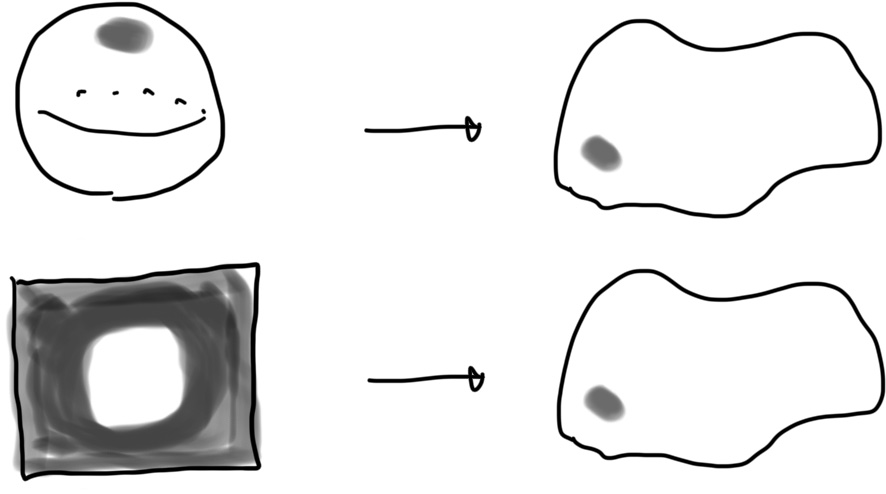
\includegraphics[width=0.5\textwidth]{homotopy}
  \caption{$f\in [S^n,X]_*$ as a map from $[0,1]^n$ to $X$.
  The shaded regions are mapped to the base point $*\in X$.}
  \label{fig:homotopy}
\end{figure}

We can define a group operation on $[S^n,X]_*$ as follows.
Take $f,g\in [S^n,X]_*$.
Regard them as maps $f,g:[0,1]^n\to X$. 
We then define $fg:[0,1]^n \to X$ by \begin{equation}
  (fg)(x_1,\ldots,x_n) = \begin{cases}
    f(2x_1,x_2,\ldots,x_n) & \text{for $x_1\in [0,1/2]$},\\
    g(2x_1-1,x_2,\ldots,x_n) & \text{for $x_1\in [1/2,1]$},
  \end{cases}
\end{equation}
see Fig.~\ref{fig:homotopy-grouplaw}.

\begin{figure}
\[
  \vcenter{\hbox{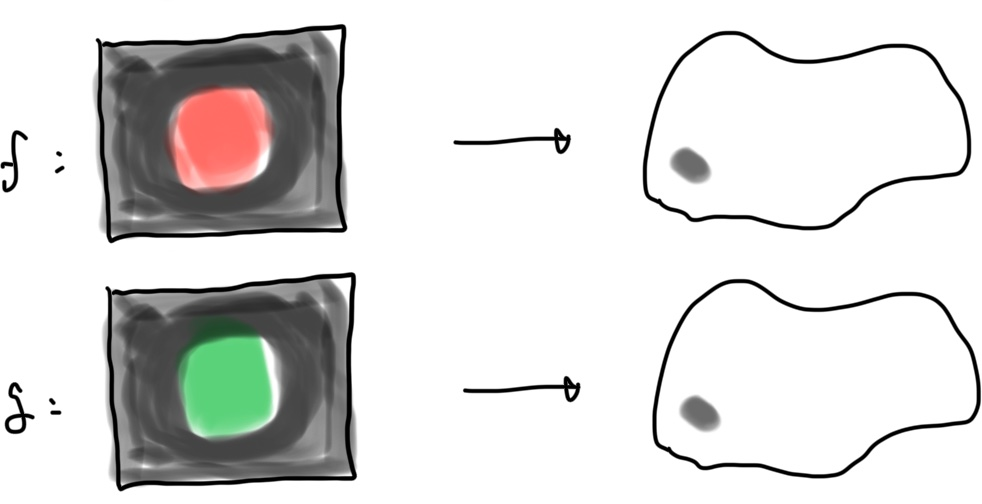
\includegraphics[width=.4\textwidth]{fg.jpg}}}\qquad
  \vcenter{\hbox{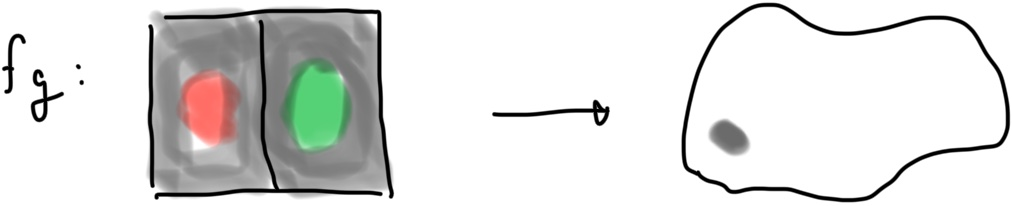
\includegraphics[width=.4\textwidth]{grouplaw.jpg}}}
\]
  \caption{The group operation $fg$ on $[S^n,X]_*$.
  The shaded regions are mapped to the base point $*\in X$.}
  \label{fig:homotopy-grouplaw}
\end{figure}
We also define $f^{-1}$ by \begin{equation}
  f^{-1}(x_1,\ldots,x_n) = 
    f(1-x_1,x_2,\ldots,x_n) 
\end{equation}
As the identity element, we use $e:S^n \to X$ which maps the entire $S^n$ to the base point $*\in X$.

\begin{proposition}
  The set $[S^n,X]_*$ for $n\ge 1$ with the group operation defined above is a group.
\end{proposition}

\begin{definition}
  The group $[S^n,X]_*$ for $n\ge 1$ is called the $n$-th homotopy group of $X$,
  and is denoted by $\pi_n(X)$.
\end{definition}

For $n=1$, $\pi_1(X)$ is also called as the fundamental group of $X$.
It is the group of closed paths from the base point to the base point,
where the group law is obtained by concatenation. 

\begin{example}
$\pi_n(\pt)=0$, where $\pt$ is a single point.
\end{example}

\begin{example}
  $\pi_n(\bR^k)=0$.
\end{example}

\begin{example}
$\pi_1(S^1)=[S^1,S^1]_*=\bZ$. 
\end{example}
This is because $f:S^1\to S^1$ is determined by how many times the image of $f$
winds around $S^1$ when we go around the source $S^1$ once.
This number is called the winding number in physics literature.
Mathematicians call it the \emph{degree} of the map.
See Fig.~\ref{fig:winding} for an illustration.

\begin{figure}[h]
  \centering
  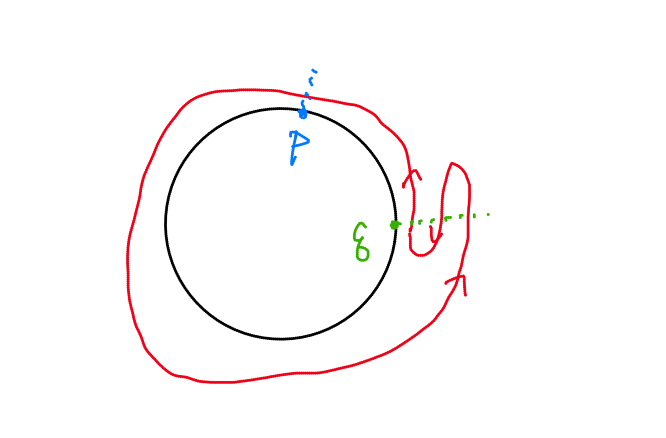
\includegraphics[width=0.3\textwidth]{winding}
  \caption{The winding number of a map $f:S^1\to S^1$.}
  \label{fig:winding}
\end{figure}

As shown there, a way to make this concept more precise is to pick a generic point $p$ in the target $S^1$,
and consider its preimage $f^{-1}(p)$.
This consists in general of a finite number of points in the source $S^1$.
We can count the number of points weighted by the local orientation of $f$ at each point.
This can be shown to be independent of the choice of $p$ in the target $S^1$,
and gives a definition of the winding number.
In Fig.~\ref{fig:winding}, the preimage of $p$ consists of one point, giving $+1$ for the winding number;
the preimage of $q$, in contrast, consists of three points,
with local orientations $+1$, $-1$, $+1$ respectively,
again giving $+1-1+1=+1$ for the winding number.


\begin{example}
  For a genus-$g$ surface $\Sigma_g$, \begin{multline}
  \pi_1(\Sigma_g)= \langle A_1,B_1,A_2,B_2,\ldots,A_g,B_g \mid \\
  A_1 B_1 A_1^{-1} B_1^{-1} A_2 B_2 A_2^{-1} B_2^{-1} \cdots A_g B_g A_g^{-1} B_g^{-1} \rangle.
  \end{multline}
\end{example}
Here $A_i$ and $B_i$ aret the closed paths starting and ending at the base point,
going around the $i$-th hole in two ways, see Fig.~\ref{fig:genus-2}.
The notation on the right hand side, $\langle a,b,\ldots \mid 
\text{relation}_1, \text{relation}_2,\ldots,\rangle$
is called a presentation of a group.

\begin{figure}[h]
  \centering
  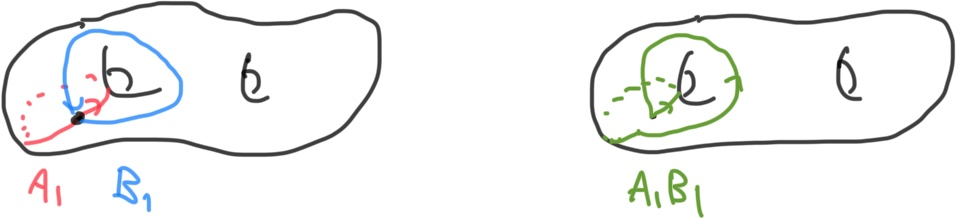
\includegraphics[width=0.6\textwidth]{genus2}
  \caption{Generators of $\pi_1(\Sigma_2)$.}
  \label{fig:genus-2}
\end{figure}

This is an Abelian group when $g=1$, i.e.~for $\Sigma_1=T^2$.
Explicitly, $\pi_1(T^2)=\bZ^2$.
But this is a non-Abelian discrete group for $g\ge 2$.

In contrast, we have:
\begin{proposition}
The group $\pi_n(X)$ is Abelian for $n\ge 2$.
\end{proposition}

For a proof, see Fig.~\ref{fig:commutativity}.
The point is that we can continuously move the nontrivial part of maps $f$ and $g$ across each other,
using the large region in $[0,1]^n$ where $f$ and $g$ are both mapped to the base point.
This is possible only when $n\ge 2$.

\begin{figure}[h]
  \centering
  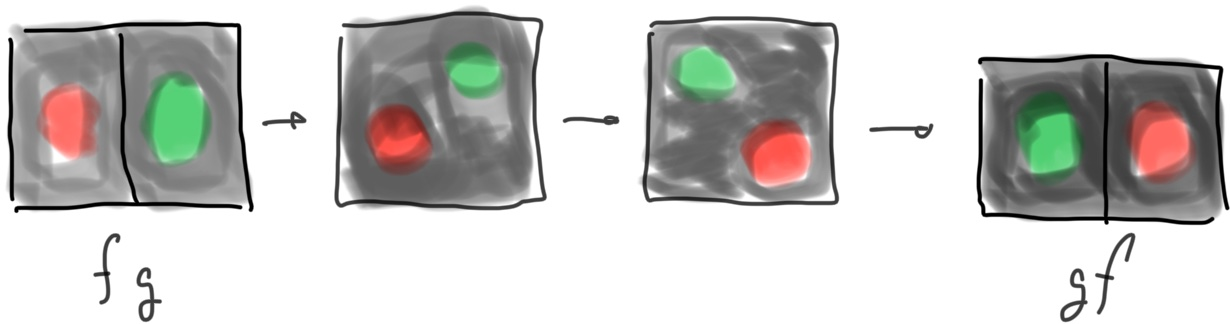
\includegraphics[width=0.6\textwidth]{commutativity}
  \caption{Commutativity of the group operation in $\pi_n(X)$ for $n\ge 2$.}
  \label{fig:commutativity}
\end{figure}

It is also sometimes useful to define the following:

\begin{definition}
We define $\pi_0(X)$ to be $[S^0,X]_*$. This is the set of connected components of $X$.
\end{definition}
Indeed, $S^0=\{*,p\}$  where $*$ is the basepoint.
Then $f:S^0\to X$ is determined by $f(p)\in X$.
We regard $f$ up to homotopy. This means that $f$ is determined by the connected component of $X$ which $f(p)$ is in.

We summarize the considerations so far:
\begin{itemize}
\item $\pi_0(X)$ is a set.
\item $\pi_1(X)$ is a group, known also as the fundamental group of $X$.
\item $\pi_{n\ge 2}(X)$ is an Abelian group.
\end{itemize}

It turns out to be useful to introduce the following notion:
\begin{definition}
  \label{def:n-connected}
A space $X$ is called \emph{connected} if $\pi_0(X)=0$,
and \emph{simply connected} if $\pi_{0,1}(X)=0$.
More generally, a space $X$ is called $n$-connected 
if $\pi_{0,\ldots,n}(X)=0$.
\end{definition}
In particular, $0$-connected means connected
and $1$-connected means simply-connected.

\subsection{Basic properties of homotopy groups}

\begin{definition}
  For a map $f:X\to Y$ and $a:S^n \to X,$ we have a map $f\circ a:S^n\to Y$.
  This determines a map $\pi_n(X)\to \pi_n(Y)$,
  which can be easily seen to be  homomorphism.
\end{definition}

\begin{proposition}
  If two maps $f,g:X\to Y$ are homotopic,
  the corresponding homomorphisms $f_*,g_*:\pi_n(X)\to \pi_n(Y)$ are the same.
\end{proposition}

In particular, if $f:X\to X$ is homotopic to identify,
$f_*:\pi_n(X)\to \pi_n(X)$ is an isomorphism.
This motivates the following definition:

\begin{definition}
  Two spaces $X$ and $Y$ are called homotopy equivalent
  if there are maps $f:X\to Y$ and $g:Y\to X$ such that 
  $f\circ g$ is homotopic to $id_Y$  
  and $g\circ f$ is homotopic to $id_X$.
\end{definition}

Then we have the following:
\begin{proposition}
  If $f: X\to Y$ gives a homotopy equivalence,
  then $f_* \pi_n(X)\to \pi_n(Y)$ is an isomorphism.
\end{proposition}
  
%We are going to define an equivalence relation between spaces
%which is much looser than homeomorphism/diffeomorphism.

When $X$ and $Y$ are homeomorphic, i.e.~if there is a 1:1 continuous map $f:X\to Y$,
taking $g=f^{-1}$ we see that $X$ and $Y$ are homotopy equivalent.
But $X$ and $Y$ being homotopy equivalent is much looser.
\begin{example}
A disk $D^2=\{|x|^2+|y|^2\le 1\}$ is homotopy equivalent to a point.
\end{example}
Indeed, let $f:D^2 \to \{(0,0)\}$ be the obvious map,
and $g:\{(0,0)\}\to D^2$ be the inclusion.
$f\circ g$ is identity.
So we need to show that $g\circ f$ is homotopic to the identity.
For this we just consider $f_s((x,y))= s(x,y)$ for $s\in [0,1]$,
and we are done.
Similarly,
\begin{example}
A disk $D^n$ in any dimension is homotopy equivalent to a point.
\end{example}

So, if we can compute $\pi_n(X)$ and $\pi_n(Y)$ for some $n$ and show $\pi_n(X)\neq \pi_n(Y)$, 
then $X$ and $Y$ are not equivalent under this very loose equivalence relation.
In particular, $X$ and $Y$ are not homeomorphic and not diffeomorphic. 
This is how the homotopy groups $\pi_n(X)$ helps in distinguishing spaces.
But we have not yet learned how to compute homotopy groups.
And this is surprisingly hard!

To get some ideas, let us enumerate some more properties:

\begin{proposition}
  $\pi_n(X\times Y) = \pi_n(X) \times \pi_n(Y)$.
\end{proposition}
This allows the computation of homotopy groups of product manifolds 
to those of the factors.

\begin{proposition}
If $X$ is a manifold, then $\pi_n(X)$ is a finitely generated group.
\end{proposition}
In particular, $\pi_n(X)$ cannot be a continuous group such as $U(N)$.

The structure of finitely generated Abelian groups are well-known:
\begin{fact}
Finitely generated Abelian group $A$ is of the form \begin{equation}
A=\bZ^n \oplus \bZ_{m_1} \oplus \cdots \oplus \bZ_{m_k}.
\label{eq:fin-gen-Abelian}
\end{equation}
\end{fact}

\begin{definition}
In the above decomposition, $\bZ^n$ is called the \emph{free part} of $A$,
and $\bZ_{m_1} \oplus \cdots \oplus \bZ_{m_k}$ is called the \emph{torsion part} of $A$.
\end{definition}

So $\pi_n(X)$ for a manifold $X$ with $n\ge 2$ is always of the form \eqref{eq:fin-gen-Abelian}.

\subsection{Facts on $\pi_n(S^m)$}

Let us have a look at concrete examples of homotopy groups.
As a starter, let us consider the homotopy groups of spheres themselves,
$\pi_n(S^m)=[S^n,S^m]_*$.

\begin{theorem}
$\pi_n(S^m) =0$ if $n<m$.
\end{theorem}
Roughly, a generic map $S^n\to S^m$ with $n<m$ has a point $p\in S^m$ not mapped from $S^n$. 
We can `push' the image of maps from that point to the base point.
So every map is homotopic to the map to the basepoint, see Fig.~\ref{fig:nm}.

\begin{figure}
  \centering
  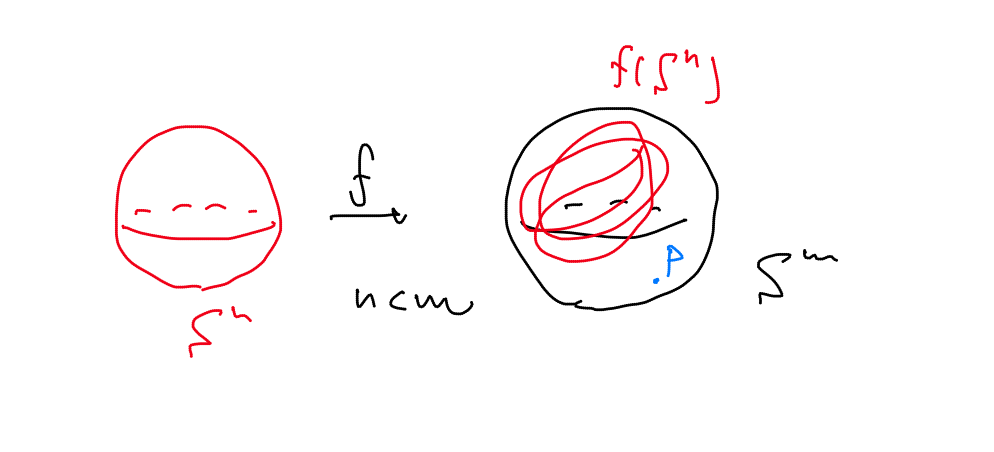
\includegraphics[width=0.6\textwidth]{nm}
  \caption{A generic map $S^n\to S^m$ with $n<m$ has a point $p\in S^m$ not mapped from $S^n$.}
  \label{fig:nm}
\end{figure}


\begin{theorem}
$\pi_n(S^n) =\bZ$.
\end{theorem}
This can be shown by considering 
the higher-dimensional version of the winding number.
For a map $f:S^n\to S^n$, 
the resulting integer is known as its \emph{degree} in mathematics.

A more interesting one is the following:
\begin{theorem}
  $\pi_3(S^2)=\bZ$. 
  Furthermore, the Hopf fibration $S^3\to S^2$ corresponds 
  to the generator of $\bZ$.
\end{theorem}

%($\nu d\nu$ where  $d\nu$ is the pull back of the volume form)


Given a map $f:S^3\to S^2$, the corresponding integer is obtained as follows.
Pick a generic point $p$ on $S^2$. 
Its inverse image $f^{-1}(p)$ is a collection of circles $C_1,\ldots, C_n$ in $S^3$.
Take another point $q$ on $S^2$.
Its inverse image $f^{-1}(q)$ is another collection of circles $C'_1,\ldots, C'_m$ in $S^3$.
We now consider \begin{equation}
\sum_{i,j} \Lk(C_i,C'_j), \label{eq:Hopf-invariant-crude}
\end{equation}
where the linking number $\Lk$ of two circles is defined in the standard way.\footnote{This appears in the integrated form of the equation of electromagnetism.
Namely, if a current $I$ flows in a loop $C$,
then the integral of the magnetic field around $C'$ 
is proportional to the linking number of $C$ and $C'$.}
One can show that this is independent under continuous deformations of $f$.
This is one definition of the Hopf invariant of $f$.
See Fig.~\ref{fig:hopf-invariant} for an illustration of the definition.

\begin{figure}
  \centering
  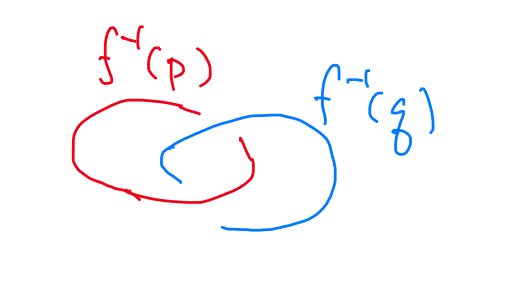
\includegraphics[width=0.4\textwidth]{hopf}
  \caption{A definition of the Hopf invariant of a map $f:S^3\to S^2$  is 
  given by considering the linking number of the inverse images of two points in $S^2$.}
  \label{fig:hopf-invariant}
\end{figure}

We drew the actual fibers of the Hopf fibration $S^1\to S^3\to S^2$ in Fig.~\ref{fig:hopf-fibers}.
By inspection, we see that two fibers have the linking number $1$. 
Therefore, the Hopf fibration $S^3\to S^2$ has the Hopf invariant $1$.

We can similarly define linking numbers of two $S^{n-1}$'s within $S^{2n-1}$ for $n>2$,
where the previous case corresponds to $n=2$.
Then, for a map $f: S^{2n-1}\to S^{n}$,
the inverse image of a generic point in $S^n$ is a $(n-1)$-dimensional space,
and then we can define a higher-dimensional Hopf invariant of $f$ as in \eqref{eq:Hopf-invariant-crude}.
Now, it is known that  \begin{equation}
\Lk (A,B)=(-1)^n \Lk (B,A)
\label{eq:Lk-sym}
\end{equation} in general, which implies that the expression \eqref{eq:Hopf-invariant-crude} gives zero when $n$ is odd.
As we see below in Proposition~\ref{prop:whitehead}, 
it is relatively easy to construct a map $S^{2n-1}\to S^n$ with Hopf invariant 2 when  $n$ is even, and therefore
\begin{theorem}
  $\pi_{4m-1}(S^{2m})$ contains a  $\bZ$ summand.
\end{theorem}

Also, by an explicit computation we can show  that \begin{proposition}
The Hopf fibrations $S^3\to S^2$, $S^7\to S^4$, $S^{15}\to S^8$,
all have Hopf invariant one.
\end{proposition}
and in fact 
\begin{theorem}
There is a map $f:S^{2n-1}\to S^n$ with Hopf invariant one
only when $n=2,4,8$.
\end{theorem}
This is a deep result in algebraic topology, known as the Hopf invariant one problem,
and the efforts to solve this question inspired many developments in the field.
We also have
\begin{proposition}
\label{prop:whitehead}
For all other $n=2m$, the minimal Hopf invariant for a map $f:S^{4n-1}\to S^{2m}$ is two.
\end{proposition}

\begin{proof}
This can be shown by constructing an example with Hopf invariant two using the Whitehead product.
Here we do not have the time to give a general theory, so let us simply give the final constructed map.

For now let $n$ be an integer, without assuming that it is even.
First, realize $S^{2n-1}$ as \begin{equation}
(S^{n-1} \times D^n) \cup (D^n \times S^{n-1}), 
\end{equation} where we identify the common boundary $S^{n-1}\times S^{n-1}$ with an appropriate orientation. 
We then define the map $f:S^{2n-1}\to S^n$ as follows,
using the map $g:D^n \to S^n$ collapsing the boundary to the basepoint:
\begin{equation}
f(p) = \begin{cases}
g(b) & \text{if}\ p=(a,b) \in S^{n-1}\times D^n ,\\
g(a) & \text{if}\ p=(a,b) \in D^{n}\times S^{n-1}.
\end{cases}
\end{equation}
Then the inverse image $f^{-1}(s)$ of $s\in S^{n-1}$ for a generic point $s$ away from the basepoint is  \begin{equation}
f^{-1}(s)= (\{s\} \times S^{n-1} ) \cup (S^{n-1} \times \{s\}),
\end{equation}
Now, we have \begin{align}
\Lk (\{s\} \times S^{n-1} ,\{t\} \times S^{n-1} )  &=0 ,\\
\Lk (\{s\} \times S^{n-1} ,S^{n-1}\times \{t\} )  &=1,
\end{align}
Using this we can compute \begin{equation}
\Lk (f^{-1}(s),f^{-1}(t)) = \begin{cases}
2 & \text{(even $n$),} \\
0 & \text{(odd $n$)} \\
\end{cases}
\end{equation}
where we used \eqref{eq:Lk-sym}.
\end{proof}



Another interesting fact is that 

\begin{theorem}
  The only free part of $\pi_n(S^m)$ is $\pi_n(S^n)\simeq \bZ$
  and the single $\bZ$ summand of $\pi_{2n-1}(S^n)$ discussed above.
  Otherwise the homotopy groups of spheres are all torsion.
\end{theorem}
  

With these basic properties covered,
let us have a look at the homotopy groups of spheres $\pi_{n+k}(S^n)$ 
for small $n$ and $k$, which are tabulated in Table~\ref{tab:pi_nS^m}.
The data are taken from 岩波数学辞典 \cite[付録, 公式 7, V]{Jiten},
which also has an English translation \cite{EDM}.
There we showed $\pi_d(S^d)\simeq \bZ$ in red,
and the $\bZ$ summand of $\pi_{2m-1}(S^m)$ in blue.


\begin{table}[h]
  \[
\begin{array}{c|cccccccccccccccccc}
  k & 0 & 1 & 2 & 3 & 4 & 5 & 6 & 7 & 8 & 9  \\
   \hline
  S^1 & \textcolor{red}{\bZ} & 0 & 0 & 0 & 0 & 0 & 0 & 0 & 0 & 0 \\
  S^2 & \cellcolor{lg} \textcolor{red}{\bZ} & \textcolor{blue}{\bZ} & \bZ_2 & \bZ_2 & \bZ_{12} & \bZ_2 & \bZ_2 & \bZ_3 & \bZ_{15} & \bZ_2  \\
  S^3 & \cellcolor{lg} \textcolor{red}{\bZ} & \cellcolor{lg} \bZ_2 & \bZ_2 & \bZ_{12} & \bZ_2 & \bZ_2 & \bZ_3 & \bZ_{15} & \bZ_2 & (\bZ_2)^2  \\
  S^4 &\cellcolor{lg}  \textcolor{red}{\bZ} & \cellcolor{lg} \bZ_2 & \cellcolor{lg} \bZ_2 & \textcolor{blue}{\bZ} \times \bZ_{12} & (\bZ_2)^2 & (\bZ_2)^2 & \bZ_{24} \times \bZ_3 & \bZ_{15} & \bZ_2  & (\bZ_2)^3\\
  S^5 & \cellcolor{lg} \textcolor{red}{\bZ} & \cellcolor{lg} \bZ_2 & \cellcolor{lg} \bZ_2 & \cellcolor{lg} \bZ_{24} & \bZ_2 & \bZ_2 & \bZ_2 & \bZ_{30} & \bZ_2 & (\bZ_2)^3  \\
  S^6 & \cellcolor{lg} \textcolor{red}{\bZ} & \cellcolor{lg} \bZ_2 & \cellcolor{lg} \bZ_2 & \cellcolor{lg} \bZ_{24} & \cellcolor{lg} 0 & \textcolor{blue}{\bZ} & \bZ_2 & \bZ_{60} & \bZ_{24}\times \bZ_2 & (\bZ_2)^3\\
  S^7 &\cellcolor{lg}  \textcolor{red}{\bZ} & \cellcolor{lg} \bZ_2 & \cellcolor{lg} \bZ_2 & \cellcolor{lg}\bZ_{24} & \cellcolor{lg} 0 &\cellcolor{lg}  0 & \bZ_2 & \bZ_{120} & (\bZ_2)^3 & (\bZ_2)^4 \\
  S^8 & \cellcolor{lg} \textcolor{red}{\bZ} & \cellcolor{lg} \bZ_2 & \cellcolor{lg} \bZ_2 & \cellcolor{lg} \bZ_{24} & \cellcolor{lg} 0 & \cellcolor{lg} 0 & \cellcolor{lg} \bZ_2 & \textcolor{blue}{\bZ}\times \bZ_{120} & (\bZ_2)^4 & (\bZ_2)^5 \\
  S^9 &\cellcolor{lg}  \textcolor{red}{\bZ} & \cellcolor{lg} \bZ_2 & \cellcolor{lg} \bZ_2 & \cellcolor{lg} \bZ_{24} & \cellcolor{lg} 0 & \cellcolor{lg} 0 & \cellcolor{lg} \bZ_2 & \cellcolor{lg} \bZ_{240} & (\bZ_2)^3 & (\bZ_2)^4 \\
  S^{10} &\cellcolor{lg}  \textcolor{red}{\bZ} & \cellcolor{lg} \bZ_2 & \cellcolor{lg} \bZ_2 & \cellcolor{lg} \bZ_{24} & \cellcolor{lg} 0 & \cellcolor{lg} 0 & \cellcolor{lg} \bZ_2 & \cellcolor{lg} \bZ_{240} & \cellcolor{lg} (\bZ_2)^2 & \textcolor{blue}{\bZ}\times (\bZ_2)^3 \\
  S^{11} &\cellcolor{lg}  \textcolor{red}{\bZ} & \cellcolor{lg} \bZ_2 & \cellcolor{lg} \bZ_2 & \cellcolor{lg} \bZ_{24} & \cellcolor{lg} 0 & \cellcolor{lg} 0 & \cellcolor{lg} \bZ_2 & \cellcolor{lg} \bZ_{240} & \cellcolor{lg} (\bZ_2)^2 & \cellcolor{lg} (\bZ_2)^3 \\
  S^{12} &\cellcolor{lg}  \textcolor{red}{\bZ} & \cellcolor{lg} \bZ_2 & \cellcolor{lg} \bZ_2 & \cellcolor{lg} \bZ_{24} & \cellcolor{lg} 0 & \cellcolor{lg} 0 & \cellcolor{lg} \bZ_2 & \cellcolor{lg} \bZ_{240} & \cellcolor{lg} (\bZ_2)^2 & \cellcolor{lg} (\bZ_2)^3 \\
\end{array}
\]
\caption{Table of $\pi_{n+k}(S^n)$ \label{tab:pi_nS^m}}
\end{table}


We clearly see more patterns in the table. 
This comes from the following general fact.
Let us start with a definition.
\begin{definition}
Given a pointed space $(X,*)$,
we define the reduced suspension $\Sigma X$ of $X$ as \begin{equation}
  \Sigma X = \frac{ X \times [0,1]}{
    X \times \{0,1\} \cup \{*\} \times [0,1]
  }. 
\end{equation}
\end{definition}

See Fig.~\ref{fig:suspension} for an illustration.
\begin{figure}
  \centering
  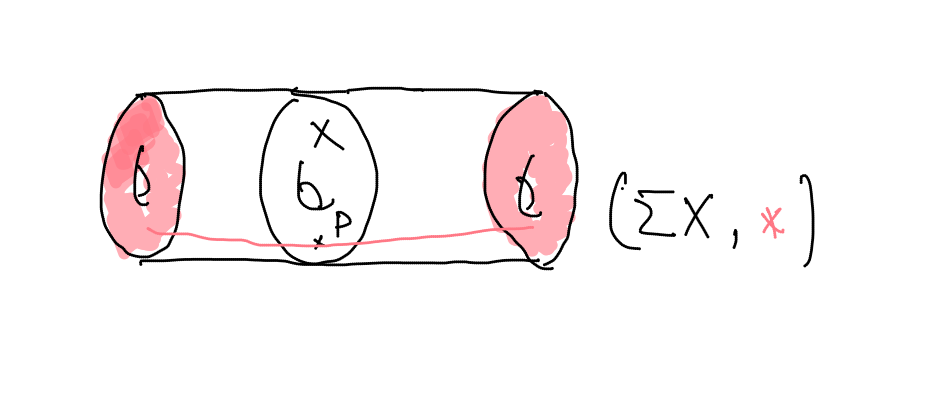
\includegraphics[width=0.5\textwidth]{suspension}
  \caption{The reduced suspension $\Sigma X$ of a space $X$.
  In the figure, we collapse all the points colored in red to a single point,
  which we take to be the basepoint.}
  \label{fig:suspension}
\end{figure}

\begin{proposition}
  $\Sigma S^n \simeq S^{n+1}$.
\end{proposition}

\begin{definition}
Given $f:X\to Y$, we define $\Sigma f:\Sigma X\to \Sigma Y$ by \begin{equation}
  (\Sigma f)([x,t]) = ([f(x),t]),
\end{equation}
where we denoted a point in $\Sigma X$ by $[x,t]$ for $x\in X$ and $t\in[0,1]$.
This determines a map \begin{equation}
[X,Y]_*\to [\Sigma X,\Sigma Y]_*.
\end{equation}
\end{definition}

In particular, when applied to $X=S^n$ and $\Sigma X=S^{n+1}$, we have 
\begin{proposition}
$\pi_n(Y)\to \pi_{n+1}(\Sigma Y)$ is a homomorphism of groups.
\end{proposition}
Furthermore, there is the Freudenthal suspension theorem:
\begin{theorem}
Suppose $Y$ is $(n-1)$-connected, i.e.~$\pi_{i<n}(Y)=0$.
Then the suspension homomorphism $\pi_k(Y)\to \pi_{k+1}(\Sigma Y)$ is an isomorphism for $k< 2n-1$ and a surjection for $k=2n-1$.
\end{theorem}
More explicitly, $\pi_{k\ge n}(\Sigma Y)=0$,
$\pi_{k}(Y)=\pi_{k+1}(\Sigma Y)$ for $k=0,1,\ldots,2n-1$,
and $\pi_{2n}(Y)\to \pi_{2n+1}(\Sigma Y)$ is surjective.

As $S^n$ is clearly $(n-1)$-connected, we see in particular 
\begin{proposition}
  $\pi_{n+k}(S^n)\to \pi_{(n+1)+k}(S^{n+1})$ 
  is an isomorphism for $k<n-1$ and a surjection for $k=n-1$.
\end{proposition}
This explains the grayed area in Table~\ref{tab:pi_nS^m}.

The homotopy groups of spheres in the grayed area 
are known as the stable homotopy groups of spheres.
More precisely, mathematicians define the following:
\begin{definition}
  We call \begin{equation}
   \pi^\text{st}_k := \lim_{n\to\infty} \pi_{n+k}(S^n)
  \end{equation}
as the $k$-th stable homotopy group of spheres,
or simply the $k$-th stem.
\end{definition}

In contrast, the homotopy groups in the ungrayed area
are known as unstable groups.
The stable homotopy groups of spheres are much easier to compute than the unstable groups.
Still, the stable homotopy groups are not quite understood.
Indeed, computing them is a major goal in algebraic topology;
currently it is known up to $k\le 83$ \cite{Isaksen}.

In this field, there is a famous principle known as the 
`Mahowald uncertainty principle' \cite[Sec.~3]{IsaksenICM},
which says 
that there is no single method 
which allows us to compute all the stable homotopy groups of spheres!
%\footnote

Before moving on to the next section,
let us discuss a particular homotopy group of spheres in the stable range
which is relevant to the Standard Model of particle physics:
\begin{example}
  $\pi_4(S^3)=\bZ_2$.
\end{example}
Using the Freudenthal suspension theorem,
we know that its generator $S^4\to S^3$ is the suspension $\Sigma p$
of the Hopf fibration $p:S^3\to S^2$.
But it is difficult to see that this map $\Sigma p$ 
generates a $\bZ_2$, and that there is no other generator.
  
\begin{remark}
The way it appears in four-dimensional physics is the following.
The weak force is described by a $SU(2)$ gauge theory,
and therefore we have an $SU(2)$ principal bundle over our spacetime.
Take a patch $\bR^4$ of the spacetime.
Then we can consider a gauge transformation \begin{equation}
  g:\bR^4\to SU(2).
\end{equation}
Let us say we don't perform any gauge transformation in the far region.
Then we essentially have a map \begin{equation}
g: S^4\to SU(2) \simeq S^3. \label{eq:su2gaugetr}
\end{equation}
Now, we have various fermions in our world.
Those charged under the weak force 
are always in the doublet representation of $SU(2)$.
A single doublet is described by a section of $\underline{\mathbf{2}}\otimes S\to M$ 
in the notation of Sec.~\ref{sec:SM};
$\underline{V}\to M$ 
is the associated vector bundle
for a representation $\rho: G \curvearrowright V$
and a principal $G$-bundle $P\to M$,
and $S\to M$ is the spin bundle.

Now, the partition function $Z_\text{single doublet}$ of a fermion in a singlet doublet representation 
of $SU(2)$ 
is known to behave under 
a gauge transformation \eqref{eq:su2gaugetr} as \begin{equation}
  Z_\text{single doublet} \to (-1)^s Z_\text{single doublet}.\label{eq:Witten-anomaly}
\end{equation}
where $s=[g] \in \pi_4(S^3) \simeq \bZ_2 \simeq \{0,1\}$;
this was found originally in \cite{Witten:1982fp}.
This means that an $SU(2)$ gauge theory with a single doublet is inconsistent, for example.

Now, in a single generation \eqref{eq:generation},
there are $3+1=4$ doublets of $SU(2)$.
Therefore, the sign \eqref{eq:Witten-anomaly} always becomes $(-1)^{4s}=+1$,
making the theory consistent.
This for example means that you cannot just change the number of colors $SU(3)$ to $SU(4)$, 
keeping everything else in the Standard Model fixed.
\end{remark}


\subsection{Long exact sequence of homotopy groups of fiber bundles}
\subsubsection{Statement}
Computing homotopy groups is hard. 
One useful technique is the long exact sequence of homotopy groups
associated to fiber bundles $F\to E\to B$.
This relates the homotopy groups  $\pi_*(F)$, $\pi_*(E)$, and $\pi_*(B)$.
This often allows us to determine one if we know the other two.
We start from the following definition:

\begin{definition}
  A sequence of groups and homomorphisms between them, \begin{equation}
  \cdots 
  \stackrel{f_{i-2}}{\longrightarrow} G_{i-1} 
  \stackrel{f_{i-1}}{\longrightarrow} G_{i}
  \stackrel{f_{i}}{\longrightarrow} G_{i+1}
  \stackrel{f_{i+1}}{\longrightarrow} \cdots
  \end{equation}
is called an exact sequence of groups if it is exact at each group, i.e.~
$f_{i-1}\circ f_i=0$ and furthermore 
\begin{equation}
 \Im f_{i}  = \Ker f_{i+1} \subset G_i \label{eq:exactness}
\end{equation}
for all $i$.
\end{definition}

This might sound a bit too opaque, so let us start with two simpler cases.
\begin{proposition}
  An exact sequence $1\stackrel{f}{\to} A\stackrel{g}{\to} 1$ means that $A\simeq 1$.
\end{proposition}
To see this, we expand the definitions of the condition $\Im f=\Ker g$.
$\Ker g$ is actually the entirety of $A$, since $g$ maps everything to $1$.
$\Im f$ is simply $\{e\}\subset A$.
Therefore, $A=\{e\}=1$.

\begin{proposition}
An exact sequence $1\stackrel{f}{\to} A\stackrel{g}{\to} B\stackrel{h}{\to} 1$ means that $A\simeq B$.
\end{proposition}
To see this, we expand the definitions of the condition $\Im f=\Ker g$ and $\Im g=\Ker h$.
As $\Im f=\{e\}$, we have $\Ker g=\{e\}$, i.e.~$g$ is injective.
As $\Ker h=B$, we have $\Im g=B$, i.e.~$g$ is surjective.
Therefore $g$ is a bijection, and $A\simeq B$.


A slight generalization is the following:
\begin{definition}
  A short exact sequence of groups is an exact sequence of groups of the following form: \begin{equation}
  1 \to A \to B \to C \to 1.
  \end{equation}
  In this case $B$ is called the extension of $C$ by $A$.
\end{definition}
Note that for Abelian groups we often use the notation $0$ instead of $1$
to denote a trivial group.

Given $A$ and $C$, $B$ is not uniquely determined.
For example, assuming all groups involved to be Abelian,
consider the short exact sequence \begin{equation}
  0 \to \bZ_2 \to A \to \bZ_2 \to 0.
\end{equation}  
Then $A$ can be $\bZ_2\times \bZ_2$ or $\bZ_4$.
In the latter case, the homomorphisms are given by \begin{equation}
0 \to \{0,1\} \xrightarrow{\times 2} \{0,1,2,3\} \xrightarrow{\mod 2} \{0,1\} \to 0.
\end{equation}
Still, a short exact sequence severely restricts the possibility of $B$ given $A$ and $C$.

Now, a general exact sequence can be decomposed into short exact sequences:
\begin{proposition}
  An exact sequence of groups\begin{equation}
    \cdots 
    \stackrel{f_{i-2}}{\longrightarrow} G_{i-1} 
    \stackrel{f_{i-1}}{\longrightarrow} G_{i}
    \stackrel{f_{i}}{\longrightarrow} G_{i+1}
    \stackrel{f_{i+1}}{\longrightarrow} \cdots
  \end{equation}
  gives rise to short exact sequences of groups \begin{equation}
    0 \to G_{i-1}/\Ker f_{i-1} \to G_i \to \Im f_{i} \to 0.
  \end{equation}
\end{proposition}

This means that, given a long exact sequence of groups,
we have a lot of information to determine the groups involved.
Let us come back to algebraic topology.
\begin{theorem}
  \label{thm:long-exact-seq-homotopy}
  Given a fiber bundle \begin{equation}
    F\stackrel{\iota}{\longrightarrow} E\stackrel{p}{\longrightarrow} B,
  \end{equation}
  we have the following long exact sequence of homotopy groups: 
  \begin{equation}\begin{array}{cccccccc}
    \cdots 
      & \stackrel{\partial}{\longrightarrow} & \pi_{n+1}(F)  
      & \stackrel{\iota_*}{\longrightarrow} & \pi_{n+1}(E)
      & \stackrel{p_*}{\longrightarrow} & \pi_{n+1}(B)  \\
      & \stackrel{\partial}{\longrightarrow} & \pi_{n}(F)  
      & \stackrel{\iota_*}{\longrightarrow} & \pi_{n}(E)
      & \stackrel{p_*}{\longrightarrow} & \pi_{n}(B)  \\
      & \stackrel{\partial}{\longrightarrow} & \cdots & &&& \cdots \\
      & \stackrel{\partial}{\longrightarrow} & \pi_{1}(F)  
      & \stackrel{\iota_*}{\longrightarrow} & \pi_{1}(E)
      & \stackrel{p_*}{\longrightarrow} & \pi_{1}(B) \\
      & \stackrel{\partial}{\longrightarrow} & \pi_{0}(F)  
      & \stackrel{\iota_*}{\longrightarrow} & \pi_{0}(E)
      & \stackrel{p_*}{\longrightarrow} & \pi_{0}(B),
      \end{array}\end{equation}
      where the last three objects are not really groups but sets,
      but the condition \eqref{eq:exactness} still holds,
      and the map $\partial$ is constructed below in Definition~\ref{def:connecting-map-homotopy}.  
\end{theorem}


\subsubsection{Use cases}
Let us have a look at some of the basic use cases. 
This shows that you can use a theorem without understanding its proof,
and without even understanding the construction of the important map $\partial$
in the statement!
This is the mindset ``math as a set of mobile apps'' I am advocating.

Consider the fiber bundle $\bZ\to \bR \to S^1$.
As $\pi_n(\bR^k)=0$, the long exact sequence simply gives
\begin{equation}
0=\pi_n(\bR)\to \pi_n(S^1)\to \pi_{n-1}(\bZ)\to \pi_{n-1}(\bR)=0
\end{equation} meaning that \begin{equation}
  \pi_n(S^1)=\pi_{n-1}(\bZ).
\end{equation} As $\pi_0(\bZ)=\bZ$ and $\pi_{n\ge 1}(\bZ)=0$,
we conclude 
\begin{example}
$
  \pi_n(S^1)=\begin{cases}
    \bZ & (n=1), \\
    0 & (n\neq 1).
  \end{cases}
$
\end{example}

Suppose $\Gamma$ acts on $S^n$ freely, with $n\ge 2$. 
We have the fiber bundle $\Gamma\to S^n\to S^n/\Gamma$.
Then we have the long exact sequence, a part of which is \begin{equation}
  \pi_1(S^n) \to \pi_1(S^n/\Gamma)\to \pi_0(\Gamma) \to \pi_0(S^n)
\end{equation} which is \begin{equation}
   0 \to \pi_1(S^n/\Gamma) \to \Gamma\to 0
\end{equation} meaning that $\pi_1(S^n/\Gamma)=\Gamma$.
Recall $\RP^n=S^n/\bZ_2$. Therefore we have \begin{equation}
  \pi_1(\RP^n)=\bZ_2.
\end{equation}
Recall further that $SO(3)=\bZ_2$. Then we have 
\begin{example}
$  \pi_1(SO(3))=\bZ_2 $.
\end{example}

Next, let us apply the long exact sequence of homotopy groups to the Hopf fibration $S^1\to S^3\to S^2$.
We learned above that $\pi_k(S^1)=0$ when $k>1$.
Therefore the long exact sequences gives \begin{equation}
  0=\pi_{k}(S^1)\to \pi_{k}(S^3)\to \pi_k(S^2)\to \pi_{k-1}(S^1)=0
\end{equation} when $k\ge 3$, meaning that 
\begin{proposition}
$  \pi_k(S^3)=\pi_k(S^2)$ for $k\ge 3$.
\end{proposition}
This in particular shows that $\pi_3(S^2)=\bZ$, the basic fact we already mentioned,
and also explains the pattern in Table~\ref{tab:pi_nS^m}
in the two columns for $S^2$ and $S^3$.

As another example, consider the computation of $\pi_1(SO(n))$.
We just saw above that $\pi_1(SO(3))=\bZ_2$.
We learned in Proposition \ref{prop:SO/SO} that there is a fiber bundle
\begin{equation}
SO(n-1)\to SO(n)\to S^{n-1}.
\end{equation} Then the long exact sequence gives
\begin{equation}
  \pi_2(S^{n-1})\to \pi_1(SO(n-1))\to \pi_1(SO(n))\to \pi_1(S^{n-1}).
\end{equation}
For $n>  3$ we have $\pi_{2}(S^{n-1})=\pi_1(S^{n-1})=0$, and therefore $\pi_1(SO(n-1))=\pi_1(SO(n))$.
Inductively, we have found 
\begin{example}
  \label{ex:pi1SOn}
$\pi_1(SO(n))=\bZ_2$ for $n\ge 3$.
\end{example}


A different part of the same long exact sequnece for $n=3$ gives \begin{equation}
  \underbrace{\pi_2(SO(2))}_{=0}
  \to \pi_2(SO(3)) 
  \to \underbrace{\pi_2(S^2)}_{\bZ}
  \stackrel{\partial}{\longrightarrow}  \underbrace{\pi_1(SO(2))}_{\bZ} \to \underbrace{\pi_1(SO(3))}=\bZ_2  \pi_1(S^2)=0.
\end{equation}
This forces $\partial:\bZ\to \bZ$ to be a multiplication by $2$,
which then means that $\pi_2(SO(3))=0$.

\begin{aside}
Before proceeding, let us see that the fact $\pi_1(SO(n))=\bZ_2$ 
can be used to show that there is a nontrivial homomorphism $\pi_4(S^3) \to \bZ_2$.
For this, pick a map $f:S^4\to S^3$, and assume that it is smooth.
As in the discussion of the Hopf invariant,
let us take the inverse image of a generic point $p$ on $S^3$, which is a disjoint union of circles.
For each circle $S^1$, pick a disk $D^2$ filling it.
In this manner, we can attach a coordinate frame (say $A$) at each point of $S^1$,
by restricting $D^2 \times \bR^4$ (with a fixed coordinate frame in $\bR^4$) on its boundary.

We also attach a (possibly different) coordinate frame at each point of $S^1$ in the following manner.
The point $p$ on $S^3$ has a natural coordinate frame in $\bR^3$.
Pulling this back to $S^1\subset S^4$ gives a coordinate frame to the transverse slice $\bR^3$ at each point of $S^1$.
Together with the direction  tangent to $S^1$, 
this gives another set of coordinate frame (say $B$).
The two coordinate frames $A$ and $B$ are related by a four-dimensional rotation $g:S^1\to SO(4)$,
which determines a class $\pi_1(SO(4))=\bZ_2=\{\pm1\}$.

Recall that the inverse image $f^{-1}(p)$ consists of a disjoint union of circles.
We compute a sign $\{\pm1\}$ for each circle as described above,
and multiply them.
This way we have a sign $\pm1$ constructed from a smooth map $f:S^4\to S^3$.
It can be shown that this is independent of various choices made,
and of continuous changes of $f$.
This defines a homomorphism $\pi_4(S^3)\to \bZ_2$.

We can explictly compute this sign for the map $f:S^4\to S^3$
obtained from the suspension of the Hopf map $S^3\to S^2$,
and it turns out to be $-1$.
This means that $\pi_4(S^3)$ is nontrivial, and has $\bZ_2$ as a quotient.

For those who know more about the algebraic topology,
what is done here is the following:
$S^4$ has a unique spin structure, and therefore
$TS^4$ restricted to $S^1$  has a natural spin structure.
The pull-back from a fixed point in $S^3$ also gives a spin structure on the normal bundle of $S^1$.
Therefore we have a spin structure on $S^1$,
which has two choices $\pm1$. 
We now multiply this number for all the circles in $f^{-1}(p)$.
\end{aside}


As a final example, consider the computation of $\pi_4(Sp(n))$.
We learned in Proposition \ref{prop:Sp/Sp} that there is a fiber bundle
\begin{equation}
  Sp(n-1)\to Sp(n)\to S^{4n-1}.
\end{equation} Then the long exact sequence gives
\begin{equation}
  \pi_5(S^{4n-1})\to \pi_4(Sp(n-1))\to \pi_4(Sp(n))\to \pi_4(S^{4n-1}).
\end{equation} For $n\ge 2$, $4n-1\ge 7$, and therefore 
\begin{equation}
  0\to \pi_4(Sp(n-1))\to \pi_4(Sp(n))\to 0,
\end{equation} i.e.~$\pi_4(Sp(n-1))=\pi_4(Sp(n))$.
As $\pi_4(Sp(1))=\bZ_2$, we inductively find that 
\begin{example}
  $\pi_4(Sp(n))=\bZ_2$.  
\end{example}
This suggests the existence of the mod-2 $SU(2)=Sp(1)$ anomaly of Witten 
carries on to higher $Sp(n)$ gauge theories,
and it indeed turns out to be the case.


\subsubsection{Idea of the proof}
Here let us give an outline of the proof of Theorem~\ref{thm:long-exact-seq-homotopy}.
To do this we first need to give the definition of the connecting map $\partial$.

\begin{figure}[h]
  \centering
  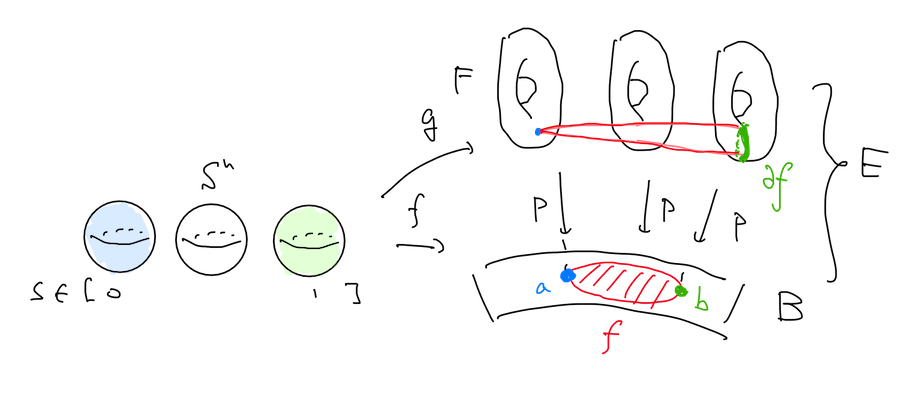
\includegraphics[width=0.8\textwidth]{connecting.png}
  \caption{The connecting map $\partial$}
  \label{fig:connecting}
\end{figure}
\begin{definition}
  \label{def:connecting-map-homotopy}
  $\partial:\pi_{n+1}(B)\to \pi_{n}(F)$ is defined as follows.
  Given a map $f:S^{n+1}\to B$, we regard it instead as a parameterized map
  \begin{equation}
  f: S^n\times [0,1] \to B
  \end{equation} such that \begin{equation}
    f(-,0):S^n\to B,\qquad
    f(-,1):S^n\to B
  \end{equation}
  are constant maps to points $a,b\in B$, respectively.
  We now consider the continuous map \begin{equation}
    \tilde f:S^n\times [0,1]\to E
  \end{equation}
  such that $p\circ \tilde f=f$ and that \begin{equation}
    \tilde f(-,0): S^n\to E
  \end{equation} is a constant map to the basepoint $*\in E$ above $a\in B$.
  Now, the image of  \begin{equation}
    \tilde f(-,1): S^n\to E
  \end{equation} contained in the fiber $F$ above $b\in B$,
  so we can define \begin{equation}
    \partial [f] := [\tilde f(-,1)]\in \pi_n(F).
  \end{equation}
\end{definition}
See Fig~\ref{fig:connecting} for an illustration of the definition.

To get a better idea of the connecting map, it is instructive 
to compute the process explicitly in a couple of examples.
For a first example, consider the fiber bundle $\bZ_2 \to S^1 \to S^1$,
where the second map is $2:1$. 
Let us study the connecting map $\partial$ at the portion \begin{equation}
  \pi_1(\bZ_2)_{=0}\to \pi_1(S^1)_{=\bZ} \to \pi_1(S^1)_{=\bZ} \stackrel{\partial}{\longrightarrow} \pi_0(\bZ_2)_{=\bZ_2} \to \pi_0(S^1)_{=\bZ}.
\end{equation}
To compute $\partial$, we take the generator of $\pi_{1}(S^1)=\bZ$,
which is the identity map $f:S^1\to S^1$.
We now consider the source $S^1$ as $S^0 \times [0,1]$ as shown in Fig.~\ref{fig:partial-example}.
We lift it to the total space.
As shown in the figure,
at the end of the process, we have the identity map $\tilde f(-,1): S^0\to \bZ_2$, generating $\pi_0(\bZ_2)=\bZ_2$.
\begin{figure}
  \centering
  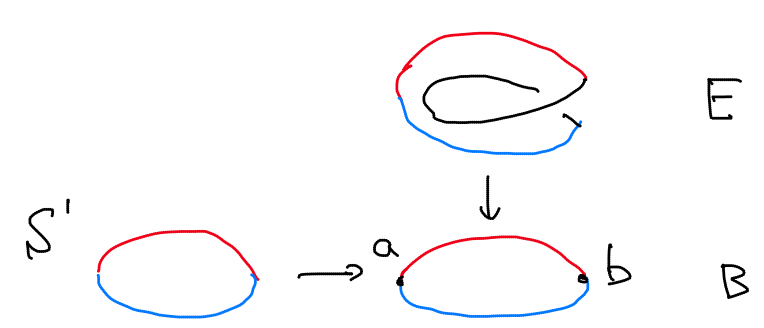
\includegraphics[width=0.6\textwidth]{partial-example}
  \caption{An illustration of the connecting map $\partial$ for the fiber bundle $\bZ_2\to S^1\to S^1$.}
  \label{fig:partial-example}
\end{figure}

For the second example, consider the following step
associated to the Hopf fibration $S^1\to S^3\to S^2$: \begin{equation}
0= \pi_2(S^3) \to \pi_2(S^2) \stackrel{\partial}{\longrightarrow} \pi_1(S^1) \to \pi_1(S^3)=0.
\end{equation}
Consider the identity map $f:S^2\to S^2$ and let us compute $\partial f$.
Let us use the polar coordinate $(\sin\theta\cos\phi,\sin\theta\sin\phi,\cos\theta)$ for $S^2$.
Then we can regard $\theta\in [0,\pi]$ as $s\in[0,1]$ used in the definition above, so $f(\phi,\theta)=(\phi,\theta)$.

Now, recall the following description \eqref{eq:Hopf-explicit} of the Hopf map $S^3\to S^2$:\begin{equation}
  (\cos(\theta/2)  e^{i \psi},
  \sin(\theta/2) e^{i(\phi+\psi)} )
  \mapsto  (\sin\theta\cos\phi,\sin\theta\sin\phi,\cos\theta).
\end{equation}
Then we can take \begin{equation}
g(\phi,\theta) := (\cos(\theta/2),\sin(\theta/2)e^{i\phi}).
\end{equation}
We indeed see that \begin{equation}
(\partial f)(\phi):= g(\phi,\pi) = (0,e^{i\phi})
\end{equation} which indeed wraps once around the fiber over $(0,0,1)$.

Now that we have some idea of the connecting map $\partial$,
let us proceed to the proof itself:

\begin{proof}
Consider first the part \begin{equation}
\pi_{n}(F) \stackrel{\iota_*}{\longrightarrow} \pi_{n}(E) \stackrel{p_*}{\longrightarrow} \pi_{n}(B).
\end{equation}
That $p_*\circ \iota_*=0$ is clear.
But not only that, we need to show that $\Im \iota_* = \Ker p_*$,
So, assume that $f:S^n\to E$ is such that $F=p\circ f: S^n\to B$ is homotopic to a trivial map.
So there is a deformation $F_s$ for $s\in [0,1]$ such that $F_0=F$ and $F_1$ is the constant map.
At each step $F_s$, we can find $f_s:S^n \to E$ such that $p\circ f_s=F_s$.
As $p\circ f_0=F_0$ is a constant map to the base, $f_0$ is actually a map to a fiber, done.

Next, consider the part \begin{equation}
  \pi_{n+1}(B)\stackrel{\partial}{\longrightarrow}\pi_{n}(F) \stackrel{\iota_*}{\longrightarrow} \pi_{n}(E).
\end{equation}
With the definition of $\partial$, the property $\Im \partial = \Ker \iota_*$ is fairly tautological.

Finally, consider the part \begin{equation}
  \pi_{n+1}(E) \stackrel{p_*}{\longrightarrow} \pi_{n+1}(B) \stackrel{\partial}{\longrightarrow} \pi_{n}(F).
\end{equation}
Again, the property $\Im p_* = \Ker \partial$ is fairly tautological.
This concludes the outline of the proof of the theorem.
\end{proof}



\subsection{Homotopy groups of Lie groups}

To use the long exact sequence of homotopy groups,
we need to know some homotopy groups to start with.
We already gave a table of $\pi_n(S^m)$ for some values of $n,m$.
Here we discuss homotopy groups of Lie groups.

\paragraph{$\pi_n(U(1))$:}
Let us start with $U(1)$. As $U(1)=S^1$, we already know $\pi_n(U(1))$.

\paragraph{$\pi_0(G)$:}
Let us then discuss non-Abelian Lie groups $G$.
For groups, $\pi_0(G)$, the set of connected components, itself is a group.
For example, $O(n)$ has two components,
the one with $\det=+1$ and another with $\det=-1$.
Then $\pi_0(O(n))=\bZ_2$. 
For the rest of this subsection, we only consider connected Lie groups,
for which $\pi_0(G)=1$.

\paragraph{$\pi_1(G)$:}
Let us next consider $\pi_1(G)$. 
\begin{fact}
$\Gamma$ is always known to be an Abelian group.
Furthermore, it is known that there always is a group $\tilde G$ with $\pi_1(\tilde G)=0$
together with a subgroup $\Gamma \subset \tilde G$ such that \begin{equation}
G=\tilde G/\Gamma.
\end{equation}
Such $\tilde G$ is known as the universal cover of $G$.
\end{fact}
Let us check that $\pi_1(\tilde G/\Gamma)=\Gamma$.
For this we consider the long exact sequence of homotopy groups associated to 
the fiber bundle $\Gamma\to \tilde G\to G$, which is \begin{equation}
\pi_1(\tilde G)\to \pi_1(G)\to \pi_0(\Gamma)\to \pi_0(\tilde G).
\end{equation}
As $\pi_1(\tilde G)=\pi_0(\tilde G)=0$, we see $\pi_1(G)\simeq \pi_0(\Gamma)\simeq \Gamma$.

The case we typically counter is $G=SO(n)$, for which $\pi_1(SO(n))=\bZ_2$ for $n\ge 3$, as we already saw in Example~\ref{ex:pi1SOn}.
The corresponding universal cover is the Spin group $Spin(n)$;
so we have \begin{equation}
\bZ_2 \to Spin(n)\to SO(n).
\end{equation}

\paragraph{$\pi_{2,3,4}(G)$:}
Consider compact Lie groups $G$ such that 
it is connected (i.e.~$\pi_0(G)=0$)
and simply-connected (i.e.~$\pi_1(G)=0$).
It is known that such groups are always a product of copies of
$\bR$ and \begin{equation}
SU(n\ge 2),\quad
Spin(n\ge 6),\quad
Sp(n\ge 2),\quad
F_4,\quad
G_2,\quad
E_6,\quad
E_7,\quad
E_8.
\label{eq:list-simple-Lie}
\end{equation}
$Spin(3)=SU(2)$, $Spin(4)=SU(2)^2$, $Spin(5)=Sp(2)$, $Spin(6)=SU(4)$
 and $Sp(1)=SU(2)$ 
were excluded from the list, as they are redundant.

The groups in \eqref{eq:list-simple-Lie} are called compact 
simple simply-connected Lie groups.

\begin{fact}
$\pi_2(G)=0$ and $\pi_3(G)=\bZ$ for groups $G$ in \eqref{eq:list-simple-Lie}.
\end{fact}

\begin{fact}
$\pi_4(G)$ for groups $G$ in \eqref{eq:list-simple-Lie} are 
either $\bZ_2$ for $G=Sp(n)$ or $0$ otherwise.
\end{fact}

\paragraph{$\pi_{n\ge 5}(G)$:}

We tabulate in Table~\ref{tab:pi_nG}
the homotopy groups of simply connected Lie groups $\pi_{n}(G)$ 
for  $3\le n\le 11$.
The data are taken from \cite[付録, 公式 7, VII]{Jiten}.
(The same set of tables should also be contained in the English translation \cite{EDM}.)

\begin{table}[ht]
  \[
  \begin{array}{c|cccccccccccccccc}
  G~\setminus~d&2&3&4&5&6&7&8&9&10&11 \\
  \hline
  \hline
  \Sp(1) &\cellcolor{lg}0&\cellcolor{lg} \bZ&\cellcolor{lg} \BZ_2 &\cellcolor{lg}\BZ_2 & \BZ_{12} &\BZ_{2} &\BZ_{2} &\BZ_{3} & \bZ_{15} &\bZ_2\\
  \Sp(2) &\cellcolor{lg}0&\cellcolor{lg}\bZ& \cellcolor{lg} \BZ_2 &\cellcolor{lg}\BZ_2 &\cellcolor{lg} 0 &\cellcolor{lg}\BZ_{} &0 &\cellcolor{lg}0 & \bZ_{120} &\bZ_2\\
  \Sp(3) &\cellcolor{lg}0&\cellcolor{lg} \bZ&\cellcolor{lg} \BZ_2 &\cellcolor{lg}\BZ_2 &\cellcolor{lg} 0 &\cellcolor{lg}\BZ_{} &\cellcolor{lg}0 &\cellcolor{lg}0 &\cellcolor{lg} 0 &\cellcolor{lg} \bZ\\
  \hline
  \SU(3) &\cellcolor{lg}0&\cellcolor{lg} \bZ&\cellcolor{lg}0 &\cellcolor{lg}\BZ &\BZ_{6} &0 &\BZ_{12} &\BZ_{3} & \bZ_{30} & \bZ_4 \\
  \SU(4) &\cellcolor{lg}0&\cellcolor{lg}\bZ&\cellcolor{lg}0 &\cellcolor{lg}\BZ &\cellcolor{lg}0 &\cellcolor{lg}\BZ &\BZ_{24} &\BZ_{2} &   \bZ_{120}\times \bZ_2 & \bZ_4 \\
  \SU(5) &\cellcolor{lg}0&\cellcolor{lg}\bZ&\cellcolor{lg}0 &\cellcolor{lg}\BZ &\cellcolor{lg} 0 &\cellcolor{lg}\BZ &\cellcolor{lg}0 &\cellcolor{lg}\BZ &  \bZ_{120}& 0 \\
  \SU(6) &\cellcolor{lg}0&\cellcolor{lg}\bZ&\cellcolor{lg}0 &\cellcolor{lg}\BZ &\cellcolor{lg} 0 &\cellcolor{lg}\BZ &\cellcolor{lg}0 &\cellcolor{lg}\BZ &  \cellcolor{lg}0 & \cellcolor{lg}\bZ  \\
  \hline
  Spin(7) &\cellcolor{lg}0&\cellcolor{lg}\bZ&\cellcolor{lg}0 &\cellcolor{lg}0 &0 &\BZ_{} &(\BZ_{2})^2 &(\BZ_{2})^2 & \bZ_8 & \bZ\times \bZ_2 \\
  Spin(8) &\cellcolor{lg}0&\cellcolor{lg}\bZ&\cellcolor{lg}0 &\cellcolor{lg}0 &\cellcolor{lg}0 &\BZ_{}^2 &(\BZ_{2})^3 &(\BZ_{2})^3 &\bZ_{24}\times \bZ_8 & \bZ\times \bZ_2    \\
  Spin(9) &\cellcolor{lg}0&\cellcolor{lg}\bZ&\cellcolor{lg}0 &\cellcolor{lg}0 & \cellcolor{lg} 0 &\cellcolor{lg}\BZ_{} &(\BZ_{2})^2 &(\BZ_{2})^2 &   \bZ_8 & \bZ\times \bZ_2\\
  Spin(10) &\cellcolor{lg}0&\cellcolor{lg}\bZ&\cellcolor{lg}0 &\cellcolor{lg}0 & \cellcolor{lg}0 &\cellcolor{lg}\BZ_{} &\cellcolor{lg}\BZ_{2} &\BZ \times \BZ_{2} &  \bZ_4 & \bZ \\
  Spin(11) &\cellcolor{lg}0&\cellcolor{lg}\bZ&\cellcolor{lg}0 &\cellcolor{lg}0 &\cellcolor{lg}0 &\cellcolor{lg}\BZ_{} &\cellcolor{lg}\BZ_{2} &\cellcolor{lg}\BZ_{2} &   \bZ_2 & \bZ\\
  Spin(12) &\cellcolor{lg}0&\cellcolor{lg}\bZ&\cellcolor{lg}0 &\cellcolor{lg}0 &\cellcolor{lg}0 &\cellcolor{lg}\BZ_{} &\cellcolor{lg}\BZ_{2} &\cellcolor{lg}\BZ_{2} &   \cellcolor{lg}0 & \bZ\times \bZ \\
  Spin(13 ) &\cellcolor{lg}0&\cellcolor{lg}\bZ&\cellcolor{lg}0 &\cellcolor{lg}0 &\cellcolor{lg}0 &\cellcolor{lg}\BZ_{} &\cellcolor{lg}\BZ_{2} &\cellcolor{lg}\BZ_{2} & \cellcolor{lg}  0 & \cellcolor{lg}\bZ\\
  \hline
  G_2 &0&\bZ&0 &0 & \BZ_{3} &0 &\BZ_{2} &\BZ_{6} &   0 & \bZ\times \bZ_2\\
  F_4 &0&\bZ&0 &0 &  0 &0 &\BZ_{2} &\BZ_{2} &0 & \bZ\times \bZ_2 \\
  E_6 &0&\bZ&0 &0 &  0 &0 &0 &\BZ & 0&\bZ \\
  E_7 &0&\bZ&0 &0 &  0 &0 &0 &0 &  0 & \bZ\\
  E_8 &0&\bZ&0 &0 &    0 &0 &0 &0 & 0 & 0
  \end{array}
  \]
  \caption{Homotopy groups of simply-connected simple Lie groups $\pi_d(G)$, $2\le d\le 11$.
   \label{tab:pi_nG}}
\end{table}

We note that the long exact sequences of homotopy groups
applied to 
\begin{equation}
\begin{array}{ccccc}
Spin(n-1)&\to& Spin(n)&\to& S^{n-1},\\
SU(n-1)&\to& SU(n)&\to& S^{2n-1},\\
Sp(n-1)&\to& Sp(n)&\to& S^{4n-1}
\end{array}
\end{equation}
lead to \begin{align}
\pi_d(Spin(n-1)) &\simeq \pi_d(Spin(n)),\\
\pi_d(SU(n-1)) &\simeq \pi_d(SU(n)),\\
\pi_d(Sp(n-1)) &\simeq \pi_d(Sp(n))
\end{align} when $d<n-2$, $d<2n-2$, $d<4n-2$, respectively.
This is consistent with the data in Table~\ref{tab:pi_nG},
and allows us to define $\pi_d(Spin(\infty))$,
$\pi_d(SU(\infty))$, and $\pi_d(Sp(\infty))$ consistently.



\subsection{Principal bundles over spheres}
\label{sec:bundle-over-sphere}
Let us use homotopy groups to classify principal bundles over spheres.

\subsubsection{Generalities}
We start from a general construction.
\begin{definition}
Given a bundle $F\to E\stackrel{p}{\longrightarrow} B$
and a map $f:X\to B$,
the pull-back bundle $p': f^*(E)\to X$ is defined as \begin{equation}
  f^*(E) = \{ (x,e)\in X\times E \mid f(x)=p(e) \},
\end{equation}
where $p'((x,e))=x$.
\end{definition}
We can explicitly introduce local trivializations of $f^*(E)$ in terms of those of $E$.
Say we are given a covering of $B$ by open sets $U_i$
and a local trivialization $f_i:p^{-1}(U_i)\to U_i\times F$ of $E$.
Denote $f_i(e)=(p(e),F_i(e))$.
We cover $X$ via $V_i:=f^{-1}(U_i)$ and define local trivializations by mapping \begin{equation}
(x,e) \in p'{}^{-1}(V_i) 
\end{equation} to \begin{equation}
(x,F_i(e)) \in V_i\times F.
\end{equation}

\begin{theorem}
\label{thm:bundle-equiv}
Given a bundle $F\to E\to B$
and two maps $f,g:X\to B$ which are homotopic to each other,
the pull-back bundles $f^*(E)$ and $g^*(E)$ are equivalent as bundles.
\end{theorem}
Recall that the equivalence of bundles were defined in Definition~\ref{def:bundle-equiv}.
The proof of this important theorem is worth looking at,
but alas we do not have the time.

\begin{proposition}
  Let $U$ be a contractible space.
  Then any bundle over $U$ is trivial.
\end{proposition}
This follows easily from the previous theorem.
Indeed, pick a point $p\in U$.
Then the identity map $id:U\to U$ is homotopic to a constant map $f:U\to U$ sending all points to $p$.
Therefore $E=id^*(E)$ is equivalent to $f^*(E)=U\times F$, which is trivial.

Let us now consider principal $G$-bundles  $G\to P\to S^n$.
We cover $S^n$ by the northern and southern hemispheres $U_+$ and $U_-$,
where we take both regions to overlap slightly around the equator.
We can trivialize the bundle over each hemisphere,
so the bundle $P$ is given by gluing
$U_+\times G$ and $U_-\times G$ over the overlap via a function
$g:U_+\cap U_-\to G$.
As $U_+\cap U_-$ is contractible to the equator $S^{n-1}$,
the bundle is determined by a map $S^{n-1} \to G$.
As two homotopic maps determine equivalent bundles,
we found that 
\begin{proposition}
  Principal $G$-bundles over $S^n$ are classified by $\pi_{n-1}(G)$.
\end{proposition}  

\subsubsection{Examples}

We have two standard examples. We start with 
$U(1)$ bundles over $S^2$.
This is classified by $\pi_1(U(1))=\pi_1(S^1)=\bZ$.

In physics, a $U(1)$ bundle is required to study electromagnetism
in topologically nontrivial cases.
We will learn later that this integer is the magnetic charge,
or equivalently the monopole flux through $S^2$.
For this, we need to introduce the concept of the connection, 
or equivalently the gauge field.
This will then lead to a differential-geometric expression for this number,
given as the integral of the magnetic field over $S^2$.

That the magnetic charge is quantized was first discovered by Dirac \cite{Dirac}.\footnote{%
It is interesting that this was done in the same year when Hopf introduced
his Hopf invariant and the Hopf fibration, $S^1\to S^3\to S^2$ in \cite{Hopf},
which was also about a nontrivial $U(1)$ bundle over $S^2$.}
Here we used a geometric argument and therefore the unit of the magnetic charge was dimensionless and was set to 1.
Later, we will see how to connect this unit to your favorite system of units of electromagnetism.
Summarizing, 
\begin{example}
$U(1)$ bundles over $S^2$ is classified by $\pi_1(U(1))=\bZ$.
This corresponds to the magnetic flux in physics.
\end{example}


Next we consider $G$-bundles over $S^3$,
where $G$ is a simple simply-connected compact Lie group $G$ such as $SU(2)$.
For these, $\pi_3(G)=\bZ$  as we learned above.

In physics,  more commonly we consider  principal bundles $P\to \bR^4$ over a flat $\bR^4$,
which we take to be a good approximation of our world.
We further assume that we are given a trivialization around infinity,
i.e.~if we remove a finite region $U\subset \bR^4$ 
where something interesting is going on,
nothing is going on the rest $U'=\bR^4 \setminus U$ of the spacetime,
and we are given a local trivialization $U'\times G$ there.
Then, we can effectively consider the region $U'$ as a single point,
and regard our bundle as coming from a principal $G$-bundle  $P\to S^4$
via a pullback, see Fig.~\ref{fig:bundle-R4}.
Then the topology of the $G$-bundle is specified by an integer $\pi_3(G)=\bZ$.
This number is known as the instanton number in physics.
Again, we will have a differential-geoemtric interpretation of this number later.

\begin{figure}[h]
  \centering
  \includegraphics[width=0.8\textwidth]{bundle-R4.png}
  \caption{Principal bundle over $\bR^4$ with a trivialization around infinity
  is given by a pull-back from $S^4$}
  \label{fig:bundle-R4}
\end{figure}

Note that the assumption that the bundle is trivial around infinity 
came from physics, and is not a mathematical necessity.
With other assumptions around infinity,
corresponding to different physics settings,
we will have other classifications.
It is also to be mentioned that the classification of bundles over $T^4$ 
is a much more difficult one.

In any case, our summary is that:
\begin{example}
For a simple simply-connected compact Lie group $G$ such as $SU(2)$,
principal $G$-bundles over $S^4$ are classified by 
$\pi_3(G)=\bZ$.
It is known in physics as the instanton number.
\end{example}

\subsubsection{Long exact sequences of homotopy groups revisited}
\label{sec:long-exact-and-bundles}
The result of this subsection can be used to have 
a different perspective 
of the long exact sequence of homotopy groups.

Let us first discuss the connecting homomorphism $\partial$.
Recall that we have a principal $H$-bundle $H\to G\to G/H$.
Pick a class $[f]\in \pi_{n}(G/H)$.
We now have a map $f:S^{n}\to G/H$.
We can use this to pull-back the $H$-bundle $G\to G/H$ to $S^n$,
resulting in a principal $H$-bundle $f^*(G)\to S^n$.
According to the classification of principal bundles over spheres,
this should be classified by a class in $ \pi_{n-1}(H)$.
In this way we have constructed a map 
$\pi_{n}(G/H)\to \pi_{n-1}(H)$.
Showing that this equals the connecting homomorphism $\partial$
given in Definition~\ref{def:connecting-map-homotopy} 
is basically expanding various definitions involved, and
nothing more.
Summarizing, we found:
\begin{proposition}
\label{prop:connecting-and-bundle}
  Given a map $f:S^{n}\to G/H$,
  the principal $G$-bundle $f^*(G)\to S^n$ 
  obtained by pulling back $G\to G/H$
  is classified by 
  the class $\partial[f]\in \pi_{n-1}(H)$.
\end{proposition}



\subsection{Topological solitons and homotopy groups}

%$G$-bundles on $S^n$ / $\bR^n$ 

%space of gauge transformations on $S^n$ / $\bR^n$

%\subsubsection{Those associated to the space of order paremeters}

Let us now come to the most traditional use of algebraic topology in physics, 
namely the study of topological solitons. 

\subsubsection{Solitons without core, also known as textures}
Suppose that we have a field on our space(time) taking values in a target space $X$,
i.e. we have a map \begin{equation}
f:\bR^D \to X.
\end{equation}
We often consider a situation where we have an (approximate) translation invariance along 
some of the directions.
Then the nontriviality of the field configuration is captured by a map 
\begin{equation}
f:\bR^d \to X.
\end{equation}
In such cases the field configuration is constant along $d'=D-d$ directions.
Let us call $d$ the \emph{codimension} of the configuration.
See Fig.~\ref{fig:codimension}.
In such cases it is meaningful to discuss its energy (or tension) per unit volume in the $d'$ direction.
For simplicity we take $d'=0$, as it does not make any difference in the analysis here,
and we simply call the energy per unit volume as the energy.

\begin{figure}[h]
\centering
  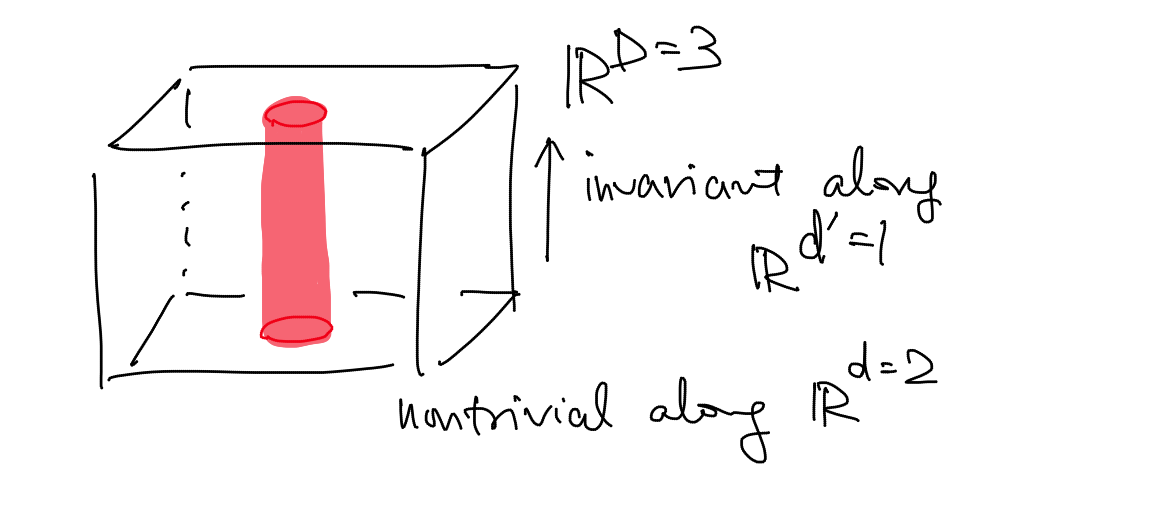
\includegraphics[width=0.7\textwidth]{codimension.png}
  \caption{A codimension-2 object in $\bR^3$ is string-like. }
  \label{fig:codimension}
\end{figure}

Now, in order not to cost an infinite amount of energy in the asymptotically far region,
most of the region of $\bR^d$ needs to map to very close to a point in the target space $X$.
We take this point the basepoint of $X$,
and then such a map is given essentially by a map from $S^d$.
See Fig.~\ref{fig:smoothsoliton}.


\begin{figure}[h]
\centering
  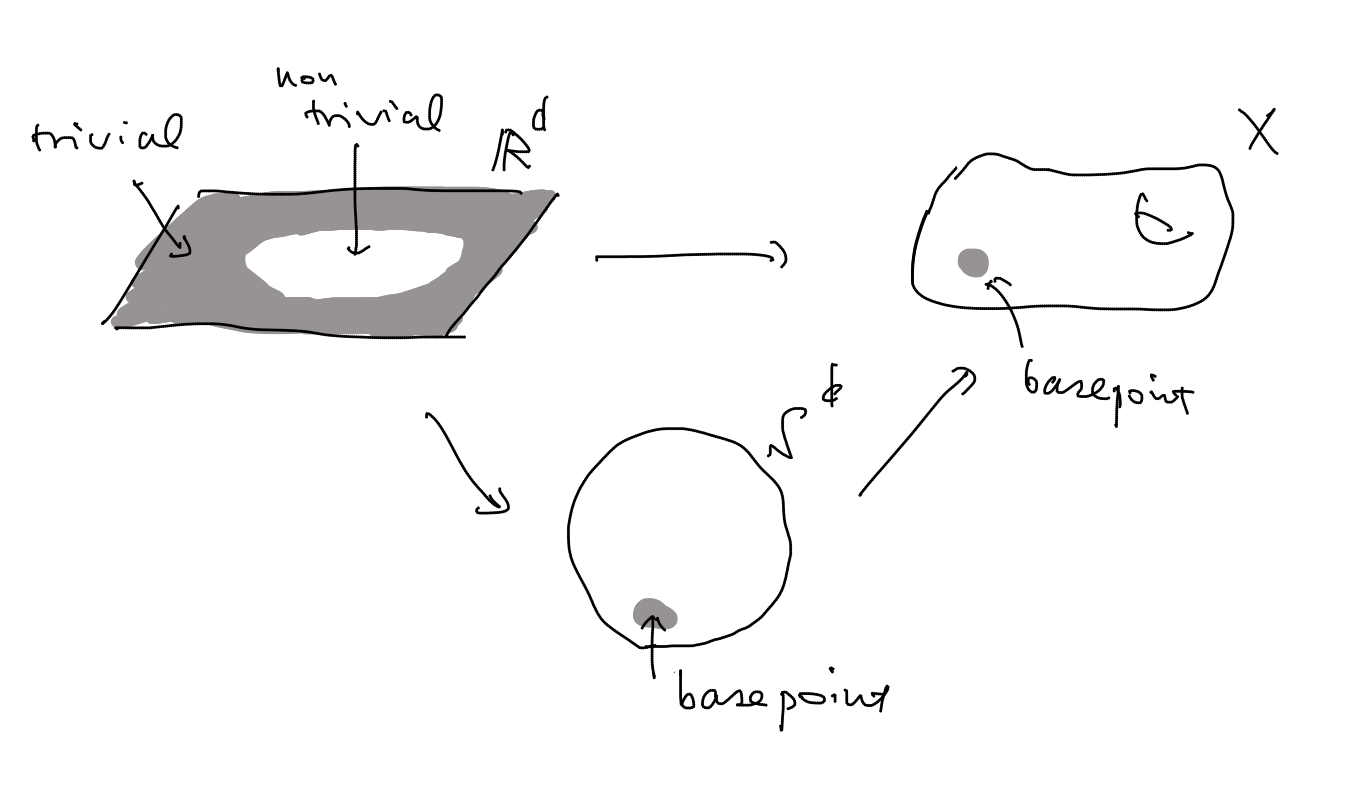
\includegraphics[width=0.7\textwidth]{smoothsoliton.png}
  \caption{A smooth, finite-energy, codimension-$d$ configuration is given by a map $S^d\to X$. }
  \label{fig:smoothsoliton}
\end{figure}

Such a configuration then determines a homotopy class $ [f]\in \pi_d(X)$.
If $[f]$ is nonzero, it cannot be removed by a continuous process,
and therefore it provides a \emph{topologically conserved charge},
and a configuration with such a topologically conserved charge is called a \emph{topological soliton}.

\begin{example}
With codimension-$3$ and the target space $S^3$, we have a Skyrmion whose charge is given by $\pi_3(S^3)=\bZ$.
\end{example}

This was first introduced by Skyrme\footnote{%
In Japan the word Skyrmion is sometimes pronounced as [\textipa{skirmion}] but I think [\textipa{sk@:mion}] is the more correct one;
after all, T. H. R. Skyrme was a British person, and I consider [\textipa{skirmion}] a hypercorrection.
As for the Ising model, I think we should use [\textipa{i:zi\ng}] instead of [\textipa{aizi\ng}],
since E. Ising is a German.
Speaking of pronunciation of names common in our field, 
the pronunciation of K\"allen in K\"allen-Lehmann spectral representation is also tricky.
I often heard high-energy physicists above my generation to pronounce it as [\textipa{tS\ae len}] or something like that.
K\"allen was Swedish,
K\"allen's grandchild was doing string theory, and I met him a couple of times.
He told me the correct pronunciation, which sounded to me  along the line of [\textipa{S\ae lien}],
which was quite different from what the Wikipedia page about the standard Swedish pronunciation.
} \cite{Skyrme:1961vq,Skyrme:1962vh} in the context of a nucleon as a soliton in the meson field.

\begin{example}
With codimension-$2$ and the target space $S^2$, we have a baby Skyrmion whose charge is given by $\pi_2(S^2)=\bZ$.
A baby Skyrmion is often simply called  Skyrmion.
\end{example}

A quick internet search gives me tons of experimental realizations of Skyrmions, 
but most of them seem to be about baby Skyrmions. 

\begin{example}
With codimension-$3$ and the target space $S^2$, we have a Hopfion, whose charge is given by $\pi_3(S^2)=\bZ$.
\end{example}

Again a quick internet search gives me some experimental realizations of Hopfions.
Another notable point is that a Hopfion charge is more subtle than a Skyrmion charge;
if you are interested, you should consult a very recent paper \cite{Chen:2022cyw},\footnote{%
I am mentioning this because I was the proud committee chair of the PhD defense of the junior author of this paper.
}
which pointed out that the Hopfion charge is associated to a non-invertible symmetry,
a hot topic in recent years.


\subsubsection{Solitons with core, better known as topological defects}

\paragraph{Generalities:}
Next let us have a look at what can be called with \emph{solitons with core}.
Consider a situation where we have a codimension-$d$ configuration
with a map to the target space $X$, where $X$ is the space of order parmeters, say.
Here we consider a situation illustrated in Fig.~\ref{fig:withcore},
where we have a map \emph{outside} of a core region $U\subset \bR^d$.
So we have a map \begin{equation}
f: \bR\setminus  U \to X.
\end{equation}

\begin{figure}[h]
\centering
  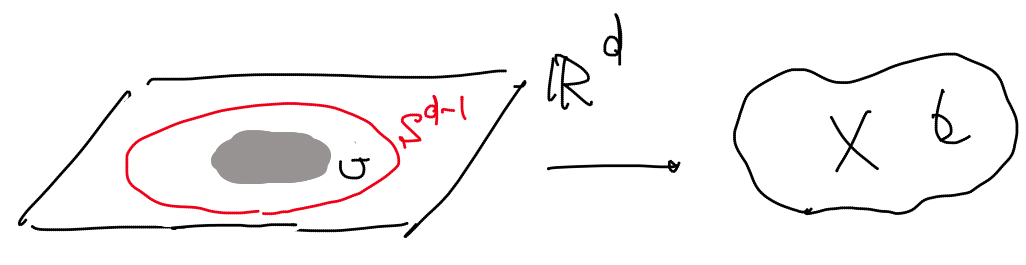
\includegraphics[width=0.6\textwidth]{withcore.png}
  \caption{A codimension-$d$ configuration with `core', given by a map $S^{d-1}\to X$. }
  \label{fig:withcore}
\end{figure}

In this case the nontriviality of such a map is measured by the homotopy class $[f]\in \pi_{d-1}(X)$
of the map $f: S^{d-1}\to X$.
Note the difference to the topological charge measured by  $\pi_d(X)$ of a smooth codimension-$d$ soliton
we discussed above.

Note that if $[f]$ is nontrivial,
it can never be continued smoothly into the entirety of $U$.
Indeed, if so, the resulting map $D^{d}\to X$ provides the homotopy to show $[f]$ is trivial.

When $[f]$ is nontrivial, then, we can't extend the map $f$ continuously to the entirety of $U$.
Inside the region $U$, we assume that some additional physics than 
simply having an order-parameter field parameterized by $X$ is going on.
This can easily happen in physics: usually the space $X$ appears only as a low-energy approximation.
It is then  that in the region $U$ the low-energy approximation breaks down.

Note also that if $[f]$ is nontrivial,
the position dependence of $f$ usually costs an infinite amount energy in the asymptotically far region.
But there are physics situations where this problem might not matter:
\begin{itemize}
\item One is that the experimental setup is finite, so the infinite energy in infinitely large $\bR^d$ might not matter;
\item Another is that when $X=G/H$ and $G$ is associated to a gauge field,
a nontrivial $G$-gauge transformation in the asymptotically far region can remove the position dependence
and therefore the associated infinite amount of energy.
\end{itemize}
In this lecture we therefore neglect these energetic consideration.

\begin{figure}[h]
\centering
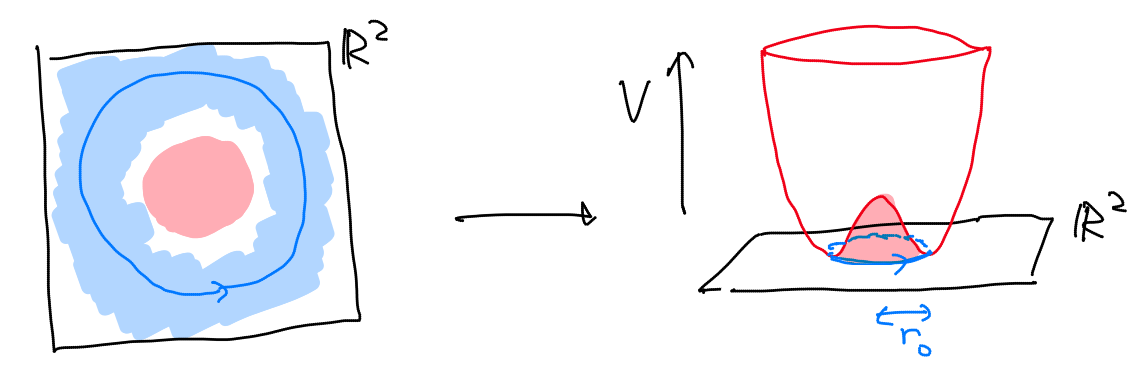
\includegraphics[width=.7\textwidth]{vortex.png}
\caption{A vortex configuration. 
In the asymptotic region, the field values are at the bottom of the potential.
In the core region, the field values come to the origin of the field space.}
\label{fig:vortex}
\end{figure}

\paragraph{Vortices:}
An example illustrating the discussion above is when $X=S^1$.
The space $S^1$ of order parameters appears as the space of potential minimum of a wine-bottle potential, as we saw in Sec.~\ref{sec:homogeneous}.
In this case we can consider a field configuration illustrated in Fig.~\ref{fig:vortex}.
In the asymptotically far region, we let the field value  to go around the potential minimum $S^1$,
as we go around the core once. 
In the core region, this $S^1$ in the field space $\bR^2$ needs to shrink. 
This is associated to the additional potential energy, but it is restricted in a finite core region in the space,
and therefore this costs only a finite amount of energy.
Note that the symmetry is broken from $G=U(1)=S^1$ to the trivial group $H=\{e\}$ at the far region,
but the full symmetry is realized at least at a point in the core region,
where the entire  symmetry $G=U(1)$ is unbroken.
In this manner, at the core of the topological soliton, the symmetry is forced to be restored. 




This vortex configuration was first introduced by Abrikosov \cite{Abrikosov:1956sx} in the context of superconductivity 
in condensed matter physics,
and by Nielsen and Olsen \cite{Nielsen:1973cs} in high energy physics. 
By now these vortices are experimentally observed, see Fig.~\ref{fig:vortex-exp}.
\begin{figure}[h]
\centering
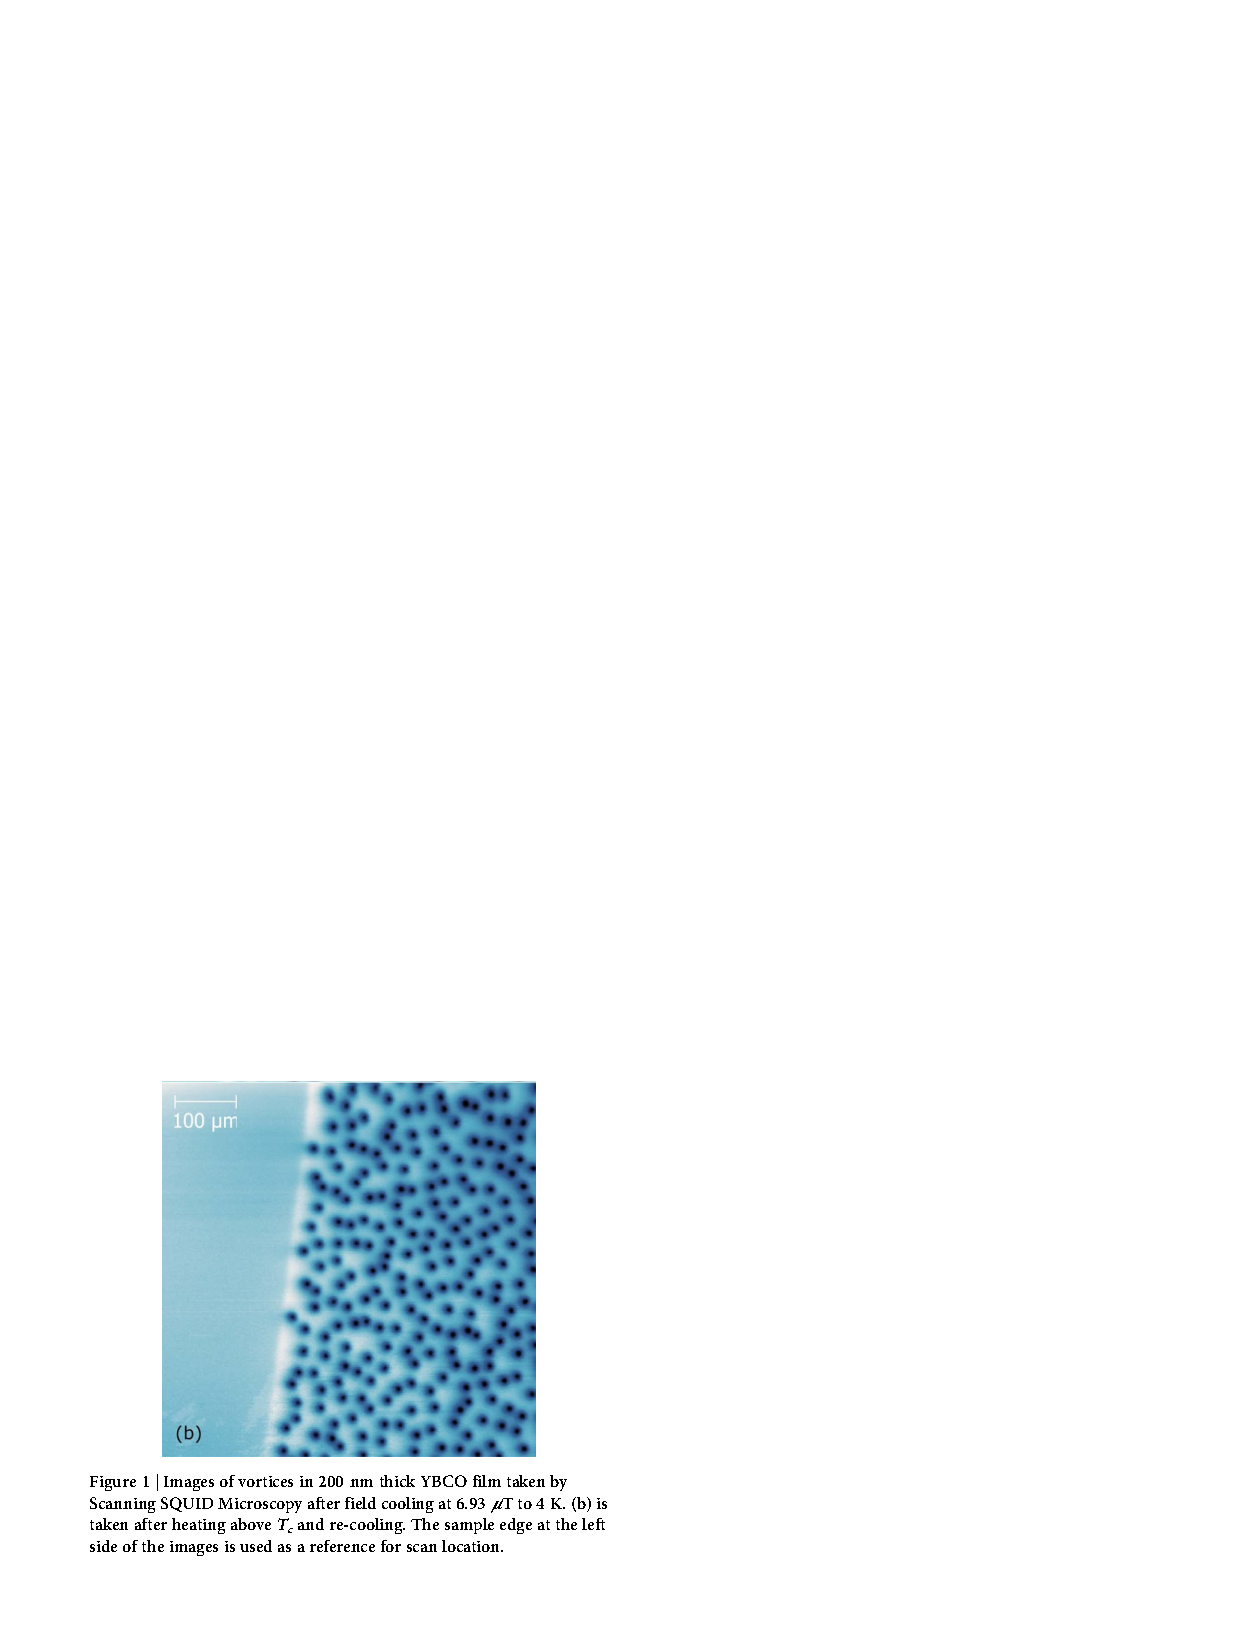
\includegraphics[width=.5\textwidth]{vortices.pdf}
\caption{A scanning SQUID-microscope view of the vortices in a superconducting material.
Taken from \cite{VortexExp}.}
\label{fig:vortex-exp}
\end{figure}
Summarizing, 
\begin{example}
A codimension-2 topological soliton with a core for the parameter space $X=U(1)$,
characterized by $\pi_1(U(1))=\bZ$,
is known as the Abrikosov/Nielsen-Olsen vortex.
\end{example}

\begin{aside}
Another application of the same line of ideas give a proof of the fundamental theorem of algebra.
Consider a degree-$n$ polynomial $P(z)$ with complex coefficients, \begin{equation}
P(z)=z^n + c_1 z^{n-1} +\cdots + c_n.
\end{equation}
Suppose that $P(z)$ does not have any zero.
Then, we can always write $P(z)=|P(z)| e^{i\theta(z)}$ unambiguously,
defining a map \begin{equation}
\theta: \bC \to S^1.
\end{equation}
Let us restrict $\theta$ to a circle $z=r e^{i\phi}$  of radius $r$ within $\bC$.
Clearly, it has winding number zero when $r$ is very small, since $P(z) \sim c_n$,
while it has winding number $n$ when $r$ is very large, since $P(z)\sim z^n$.
As the winding number should be constant when $r$ is continuously varied,
this cannot happen.
Therefore $P(z)$ has at least one zero, say at $z=z_0$.
Therefore $P(z)=(z-z_0)Q(z)$.

If you prefer a physics analogy, 
say that $P(z)$ gives a field configuration.
Then, away from cores, we have a map to $S^1$.
At large $r$, the winding number is $n$. 
Therefore, there should be at least one core, when $P(z)$ vanishes.
\end{aside}


Coming back to physics interpretations of algebraic topology,
let us further identify this $G=U(1)$ is identified with the electromagnetic $U(1)$.
In this case, we can show that the core region contains a unit magnetic flux in the following manner;
we will give a more traditional approach using the vector potential later.
To measure the magnetic flux topologically,
let us try to put this configuration on an $S^2$, and use the result in Sec.~\ref{sec:bundle-over-sphere}.
We first put this configuration on a large $D^2$, which we consider to be the northern hemisphere.
We have a region $B$ around the equator $L$ 
%(given in blue in Fig.~\ref{fig:R2S2})
where we have a product bundle $B \times S^1$.
For the sake of generality,
let us say that the field value  goes around $S^1$ $N$ times, when we go around the equator once.

We also introduce another $D^2$, which we use as the southern hemisphere.
On it, we consider a trivial bundle $D^2\times S^1$ and a constant section.
To paste the two hemispheres so that the sections match, 
we need to use a $U(1)$ gauge transformation $g:S^1\to S^1$ which also goes around $S^1$ $N$ times.
This means that on the resulting $S^2$, the $U(1)$ bundle
is characterized by $N\in \pi_1(S^1)\simeq \bZ$,
and therefore has the magnetic charge $N$.
See Fig.~\ref{fig:vortex-flux} for an illustration.

\begin{figure}[h]
\centering
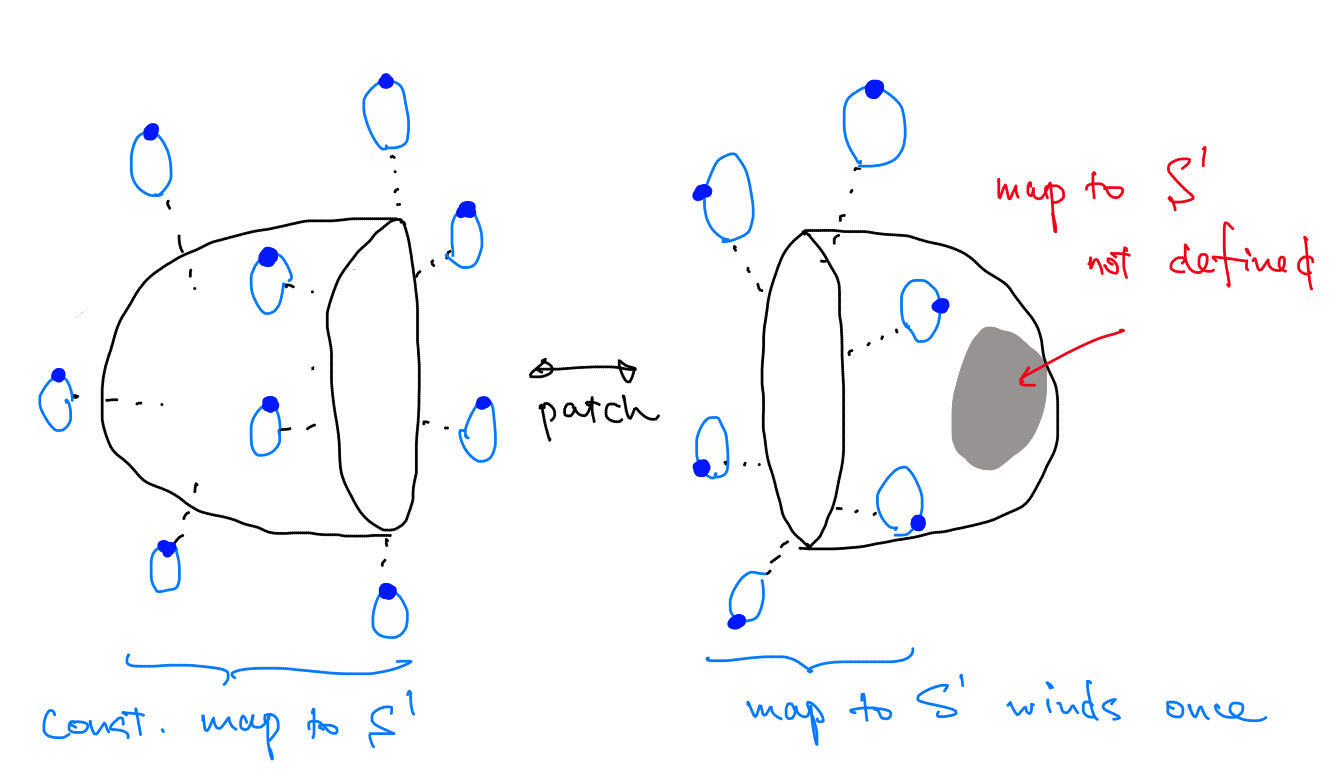
\includegraphics[width=.8\textwidth]{vortex-flux.png}
\caption{To measure the magnetic flux, we can put a vortex configuration on $S^2$.
This requires a nontrivial gauge transformation around the equator.}
\label{fig:vortex-flux}
\end{figure}


\paragraph{Instanton particles:}

Although not directly relevant to nature,
at least at the mathematical level we can replace $\pi_1(U(1))=\bZ$ with $\pi_3(SU(2))$,
and consider a codimension-4 particle in a $(4+1)$-dimensional system:
\begin{example}
A codimension-4 topological soliton with a core for the parameter space $X=SU(2)$
can be considered.
\end{example}
For example, a D0-brane within a stack of D4-branes has such a realization,
where D$p$-brane is a $(p+1)$-dimensional solitonic objects in string theory.

Note that our argument in Sec.~\ref{sec:long-exact-and-bundles} 
shows that the core of this soliton has the instanton charge $1$, 
again characterized by the same $\pi_3(SU(2))=\bZ$.
For this reason this is often called an `instanton-particle' in string theory.

\paragraph{Monopoles:}

Our final example is the following:
\begin{example}
A codimension-3 topological soliton with a core for the parameter space $X=S^2$
is known as 't Hooft-Polyakov monopole.
\end{example}
This was first introduced by 't Hooft \cite{tHooft:1974kcl} and Polyakov \cite{Polyakov:1974ek}.
When we regard $S^2=SU(2)/U(1)$
and consider a gauge theory setup where we have a larger group $SU(2)$ broken to $U(1)$,
and identify $U(1)$ as the electromagnetic gauge group,
it has a magnetic charge on $S^2$,
whose charge is characterized by Proposition~\ref{prop:connecting-and-bundle} 
via the image of $\pi_2(SU(2)/U(1))$ to $\pi_1(U(1))$ in the part of
 the long exact sequence of  homotopy groups associated to the bundle $U(1)\to SU(2)\to SU(2)/U(1)$: \begin{equation}
 \pi_2(SU(2)/U(1)) \to \pi_1(U(1)) \to \pi_1(SU(2))\to \pi_1(SU(2)/U(1))
\end{equation} which is \begin{equation}
 \bZ \to \bZ \to 0 \to 0.
\end{equation}
The exactness forces the first map to be the identity.
Therefore, the minimal 't Hooft-Polyakov monopole characterized by $1\in \pi_2(S^2)=\bZ$
has the unit magnetic charge $1\in \pi_1(U(1))$.

In contrast, if we regard $S^2=SO(3)/SO(2)$
and identify $SO(2)$ as the electromagnetic gauge group,
the magnetic charge is characterized by the same token by studying \begin{equation}
 \pi_2(SU(2)/U(1)) \to \pi_1(SO(2)) \to \pi_1(SO(3)) \to \pi_1(SU(2)/U(1))
\end{equation} which is \begin{equation}
 \bZ \to \bZ \to \bZ_2 \to 0.
\end{equation}
The exactness forces the first map to be a multiplication by $2$.
Therefore, the minimal 't Hooft-Polyakov monopole characterized by $1\in \pi_2(S^2)=\bZ$
has the magnetic charge $2\in \pi_1(SO(2))$, which has twice the minimal value.

This subtle difference of the magnetic charge of the 't Hooft-Polyakov monopole by a factor of two
between an $SU(2)$ gauge theory and an $SO(3)$ gauge theory
 plays an important role in the modern study of topological properties of gauge theories.
 See e.g.~\cite{Aharony:2013hda}.

\subsubsection{Some suggested questions}



\begin{question}
The superfluid Helium 3 A-phase and B-phase have various topological solitons characterized by $\pi_d(G/H_\text{A})$
and $\pi_d(G/H_\text{B})$ we discussed in Example~\ref{ex:helium3}.
Learn about it. 
\end{question}

The description of $\pi_d(G/H_\text{A})$ is a good exercise of the long exact sequence we learned above.
I am not familiar with the status of experimental verification of these predicted topological solitons.

\begin{question}
Look for an experimental paper on a topological soliton, either with or without core, and study it.
\end{question}
There are tons of papers of this kind. Find one, have a look, and discuss the content!

\begin{question}
Note that $\pi_d(X)$ can correspond to a codimension-$d$ texture (i.e.~a topological soliton without core)
and also to a codimension-$(d+1)$ topological defect (i.e.~a topological soliton with core).
In general they can coexist, but I do not know any concrete examples.
Are there any nice examples, preferably with some experimental realization?
\end{question}

\section{Differential forms and de Rham cohomology}
\label{sec:deRham}

\subsection{Differential forms}
Given a smooth manifold $M$, we have introduced its cotangent bundle $T^*M$.
On a patch $M\supset U \xrightarrow{f} \bR^n$ with $f(m)=(x^1,\ldots,x^n)$,
the fiber had a basis $dx^i$.
Introduce another patch $M\supset \tilde U \xrightarrow{\tilde f} \bR^n$ with $\tilde f(m)=(\tilde x^1,\ldots,\tilde x^n)$.
Then the basis $d\tilde x^a$ of the fiber of $T^*M$ over $\tilde U$ is related to the basis $dx^i$ on the overlap $U\cup \tilde U$ \begin{equation}
  d\tilde x^a = \sum_{j} \frac{\partial \tilde x^a}{\partial x^j} dx^j.
\end{equation}

A section of $T^*M$ has an expression \begin{equation}
  \omega = \sum_i \omega_i(m) dx^i
\end{equation} on a patch $U$, where $\omega_i$ is a function $U\to \bR$.
On another patch $\tilde U$, we have \begin{equation}
  \omega = \sum_a \tilde\omega_a(m) d\tilde x^a
\end{equation} where $\tilde\omega_a$ is a function $\tilde U\to \bR$.

Combining the definitions above, we find \begin{equation}
\omega_i(m)=\sum_a \tilde\omega_a(m) \frac{\partial \tilde x^a}{\partial x^i}.
\end{equation}
This means that the section $\omega$ of the cotangent bundle $T^*M$ is simply another name for the covariant vector field in general relativity.

\begin{definition}
  Given a vector space $V$ of dimension $n$ with a basis $e^1,\ldots,e^n$, 
  its antisymmetric tensor power $\wedge^p V$ is the vector space with the basis \begin{equation}
    e^{i_1}\wedge \cdots \wedge e^{i_p}
  \end{equation} where $1\le i_1<\cdots<i_p\le n$.
  It has the dimension $\binom{n}{p}$.
\end{definition}

You don't have to think what \emph{exactly is} $e^1\wedge e^2$.
It is simply a symbol which you can manipulate, following the rules below.
\begin{definition}
Between two elements of $V$,
we define the symbol $\wedge$ to satisfy the following rules:
\begin{align}
  e^i\wedge e^j &= - e^j\wedge e^i,\\
  \sum_i (a_i e^i) \wedge \sum_j (b_j e^j) &= \sum_{i,j} a_i b_j e^i\wedge e^j.
\end{align}
More generally, we demand $\wedge$ to be an associative product operation,
so that $a\wedge b\in \wedge^{p+q} V$ for $a\in \wedge^p V$ and $b\in \wedge^q V$.
\end{definition}
That these rules do not run into contradiction is a somewhat nontrivial fact,
but we will not go into the details here.
\begin{remark}
  Note that $\alpha\wedge \beta=(-1)^{pq}\beta\wedge \alpha$ when  $\alpha\in \wedge^p V$ and $\beta\in \wedge^q V$.
We also note that we often simply write $\alpha\beta$ instead of $\alpha\wedge \beta$, if it is clear from the context.  
\end{remark}


By performing these operations at each fiber, we have $\wedge^p T^*M$,
whose section on a patch has the form \begin{align}
  \omega   &=
  \sum_{i_1<\cdots<i_p} \omega_{i_1\cdots i_p}(m) dx^{i_1}\wedge \cdots \wedge dx^{i_p} \\
  &= 
  \frac{1}{p!} \sum_{i_1,\ldots,i_p} \omega_{i_1\cdots i_p}(m) dx^{i_1}\wedge \cdots \wedge dx^{i_p} 
\end{align}
where $\omega_{i_1\cdots i_p}$ is a function $U\to \bR$ 
and we require
$\omega_{i_1,\ldots,i_p}(m)$ to be antisymmetric under the exchange of $i_1,\ldots,i_p$
in the second line above.

\begin{definition}
A section of $\wedge^p T^*M$ is called a differential $p$-form on $M$.
In physics it is also called an antisymmetric tensor field with $p$ indices.
The space of all $p$-forms on $M$ is denoted by $\Omega^p(M)$.
\end{definition}

We usually drop the adjective `differential' and simply call them $p$-forms.
Note that a zero-form is simply a function on $M$,
and a one-form is a covariant vector field.
Note also that given a $p$-form $\omega$ and a $q$-form $\eta$,
$\omega\wedge\eta$ is a $(p+q)$-form.


Let us now introduce the exterior derivative $d$.
\begin{definition}
For a function $f:M\to \bR$, we define its exterior derivative as \begin{equation}
df = \sum_i \frac{\partial f}{\partial x^i} dx^i
\end{equation} where $x^i$ is a coordinate on a patch $U$.
\end{definition}
Note that $df$ is defined on individual patches $U$ of $M$.
That they agree on the overlaps $U\cap \tilde U$ follows easily from the rules given above.

\begin{definition}
  For a $p$-form $\omega$, its exterior derivative $d\omega$ is a $(p+1)$-form \begin{equation}
    d\omega = \sum_{i_1<\cdots<i_p} (d\omega_{i_1\cdots i_p}) \wedge dx^{i_1}\wedge \cdots \wedge dx^{i_p}.
  \end{equation}
\end{definition}
Again this is defined on a single patch; one needs to show that they agree on the overlaps.

\begin{proposition}
  The exterior derivative $d$ satisfies the following properties.
  \begin{itemize}
    \item $d$ is linear: $d(a \omega + b \eta) = a d\omega + b d\eta$ for  $a,b\in \bR$.
    \item $d$ satisfies the Leibniz rule: $d(\omega\wedge \eta) = d\omega \wedge \eta + (-1)^p \omega \wedge d\eta$ for a $p$-form $\omega$ and a $q$-form $\eta$.
    \item $d$ satisfies $d^2=0$. 
  \end{itemize}
\end{proposition}
In mathematics an operator which is linear, satisfies the Leibniz rule, and satisfies $d^2=0$ is called a \emph{differential}.

On $M=\bR^3$, differential forms and $d$ are often introduced in the context of electromagnetism, written with vector calculus.
Given a scalar $f:\bR^3\to \bR$, we have \begin{equation}
df = \frac{\partial f}{\partial x}dx + \frac{\partial f}{\partial y}dy + \frac{\partial f}{\partial z}dz
\end{equation}
and so its three components can be identified with \begin{equation}
(\frac{\partial f}{\partial x},\frac{\partial f}{\partial y},\frac{\partial f}{\partial z}) = \nabla f = \mathrm{grad}\ f.
\end{equation}

Given a vector field $\mathbf{E}$, package it as a one-form \begin{equation}
E= E_x dx + E_y dy + E_z dz.
\end{equation}
Then \begin{equation}
dE = \left(\frac{\partial E_z}{\partial y} - \frac{\partial E_y}{\partial z}\right) dy\wedge dz
+ \left(\frac{\partial E_x}{\partial z} - \frac{\partial E_z}{\partial x}\right) dz\wedge dx
+ \left(\frac{\partial E_y}{\partial x} - \frac{\partial E_x}{\partial y}\right) dx\wedge dy
\end{equation}
whose three components can be identified with \begin{equation}
\left(\frac{\partial E_z}{\partial y} - \frac{\partial E_y}{\partial z},\frac{\partial E_x}{\partial z} - \frac{\partial E_z}{\partial x},\frac{\partial E_y}{\partial x} - \frac{\partial E_x}{\partial y}\right) = \nabla\times \mathbf{E} = \mathrm{rot}\ \mathbf{E}.
\end{equation}

Given a vector field $\mathbf{B}$, we can also package it as a two-form \begin{equation}
B = B_x dy\wedge dz + B_y dz\wedge dx + B_z dx\wedge dy.
\end{equation}
Then \begin{equation}
  dB=(\frac{\partial B_x}{\partial x} + \frac{\partial B_y}{\partial y} + \frac{\partial B_z}{\partial z}) dx\wedge dy\wedge dz
\end{equation}
whose single component can be identified with \begin{equation}
\frac{\partial B_x}{\partial x} + \frac{\partial B_y}{\partial y} + \frac{\partial B_z}{\partial z} = \nabla\cdot \mathbf{B} = \mathrm{div}\ \mathbf{B}.
\end{equation}
Then our single equation $d^2=0$ corresponds to the three statements \begin{equation}
  \mathrm{rot} \circ \mathrm{grad} = 0,\quad
  \mathrm{div} \circ \mathrm{rot} = 0.
\end{equation}

On $M=\bR^4$,
the scalar potential $\phi$ and the vector potential $\mathbf{A}$ of the Maxwell theory
can be neatly packaged in a one-form \begin{equation}
A = \phi dt + A_x dx + A_y dy + A_z dz.
\end{equation}
Then $F=dA$ is a two-form \begin{equation}
  \begin{aligned}
  F &= 
 E_x dt\wedge dx + E_y dt\wedge dy + E_z dt\wedge dz \\
&\quad + B_x dy\wedge dz + B_y dz\wedge dx + B_z dx\wedge dy .
\end{aligned}
\end{equation}
As $d^2=0$, we have $dF=0$, which gives two of the four Maxwell equations:
\begin{equation}
\mathrm{rot}\ \mathbf{E} = -\frac{\partial \mathbf{B}}{\partial t},\quad
\mathrm{div}\ \mathbf{B} = 0.
\end{equation}

On a general manifold $M$, the field strength $F$ is a two-form.
The vector potential $A$ is \emph{not} quite a one-form, however,
as we will soon see below.

\subsection{Pull-back and the integration of differential forms}

In vector analysis, the following Stokes theorems are often used:
\begin{align}
\int_L (\mathrm{grad}\ f) \cdot d\vec x &= f(q)-f(p), \label{eq:grad-stokes}\\
\int_D (\mathrm{rot}\ \vec A) \cdot d\vec \sigma &= \int_{\partial D} \vec A \cdot d\vec x, \label{eq:rot-stokes}\\
\int_B (\mathrm{div}\ \vec E) dV &= \int_{\partial B} \vec E \cdot d\vec \sigma,\label{eq:div-stokes}
\end{align}
where $L$ is a curve starting at $p$ and ending at $q$,
$D$ is a two-dimensional surface with unit normals $\vec \sigma$ given at each point,
and $B$ is a three-dimensional region with volume element $dV$.

These are all special cases of the Stokes theorem for differential forms.
To state it, we first need to introduce the integration of a differential form.
On a smooth manifold $M$ of dimension $n$,
$n$-forms are also known as the top forms, 
since $(n+1)$-forms and above are automatically zero.
On a patch $U$, an $n$-form $\omega$ is given by \begin{equation}
\omega = \omega(m) dx^1\wedge \cdots \wedge dx^n
\end{equation} where $\omega(m)$ is a function $U\to \bR$.
On a different patch $\tilde U$, we have \begin{equation}
\omega = \tilde \omega(m) d\tilde x^1\wedge \cdots \wedge d\tilde x^n
\end{equation} where $\tilde \omega(m)$ is a function $\tilde U\to \bR$,
and \begin{equation}
\omega(m) = \tilde \omega(m) \det \frac{\partial \tilde x^i}{\partial x^j}.
\end{equation}
This means that the $n$-form $\omega$ is a density on $M$,
and it makes sense to integrate $\omega$ over $M$.
\begin{definition}
Take a smooth manifold $M$ of dimension $n$.
Let $\omega$ be an $n$-form on $M$.
Its integral $\int_M \omega$ is defined by covering $M$ by non-overlapping patches $U$,
and summing up $\int_U \omega(m) dx^1\wedge \cdots dx^n$ over all patches.
\end{definition}

To state the Stokes theorem in general,
we need to discuss the integral of a $p$-form on $M$ on a $p$-dimensional submanifold $N$ of $M$.
For this, we need to introduce the pullback of a differential form.
\begin{definition}
Take a map $f:X\to Y$ between two manifolds,
of dimension $m$ and $n$, respectively.
Take a $p$-form $\omega$ on $Y$.
Its pull-back $f^*(\omega)$ is a $p$-form on $X$ defined as follows.
Let $U\subset X$ be mapped to $f(U)\subset V \subset Y$,
with coordinates $x^{i=1,\ldots,m}$ and $y^{a=1,\ldots,n}$ for $U$ and $V$, respectively.
$\omega$ on $Y$ is given as \begin{equation}
\omega = \sum_{a_1<\cdots<a_p} \omega_{a_1\cdots a_p}(y) dy^{a_1}\wedge \cdots \wedge dy^{a_p}.
\end{equation}
Then $f^*(\omega)$ on $U$ is given by the same expression as above,
where $y^a$ are now understood to be the composition $y^a\circ f: U\to \bR^n$.
The pull-back is a map \begin{equation}
f^*: \Omega^p(Y)\to \Omega^p(X).
\end{equation}
\end{definition}
That this definition is well-defined and does not depend on the patches chosen 
needs some work, but is a straightforward computation.
Note also that the direction of the arrow $X\to Y$ and the direction of the arrow $f^*: \Omega^p(Y)\to \Omega^p(X)$ are opposite to each other.

\begin{proposition}
  Given $f:X\to Y$ and $g:Y\to Z$,
  we have \begin{equation}
  f^*: \Omega^p(Y)\to \Omega^p(X),\quad
  g^*: \Omega^p(Z)\to \Omega^p(Y),\quad
  (g\circ f)^* : \Omega^p(Z)\to \Omega^p(X).
  \end{equation}
  They satisfy $(g\circ f)^* = f^*\circ g^*$.
\end{proposition}

\begin{proposition}
The pull-back $f^*$ satisfies the following properties.
\begin{itemize}
\item $f^*$ is linear: $f^*(a\omega + b\eta) = a f^*(\omega) + b f^*(\eta)$ for $a,b\in \bR$.
\item $f^*$ preserves the product: $f^*(\omega\wedge \eta) = f^*(\omega)\wedge f^*(\eta)$.
\item $f^*$ commutes with the exterior derivative: $f^*(d\omega) = d(f^*(\omega))$.
\end{itemize}
\end{proposition}

Because of this property, we can typically forget where the form is defined.
Writing $f^*(\omega)$ as $\omega$, when $f$ is understood from the context,
does not cause any trouble.

\begin{definition}
Given a $p$-form $\omega$ on $M$ and a $p$-dimensional submanifold $N$ of $M$,
we define the integral of $\omega$ over $N$ as \begin{equation}
\int_N \omega := \int_N \iota^*(\omega)
\end{equation}
where $\iota:N\to M$ is the inclusion map.
\end{definition}

The general Stokes theorem is the following:
\begin{proposition}
Take a $(p+1)$-dimensional submanifold $N$ of $M$, possibly with a boundary $\partial N\neq \varnothing$.
Take a $p$-form $\omega$ on $M$.
Then we have \begin{equation}
\int_N d\omega = \int_{\partial N} \omega.
\end{equation}
\end{proposition}
It is a good exercise to show that all the standard Stokes theorems in vector analysis, \eqref{eq:grad-stokes}, \eqref{eq:rot-stokes}, and \eqref{eq:div-stokes}, 
are special cases of this construction on $\bR^3$.
For example, given a curve $C$ in $\bR^3$ starting from $p$ and ending at $q$,
its boundary $\partial C$ consists of points $p$ and $q$,
where the orientation of $p$ is negative and that of $q$ is positive.
Then, given a function $f$, we have \begin{equation}
\int_C df = \int_{\partial C} f = \int_q f - \int_p f = f(q)-f(p).
\end{equation}

\subsection{de Rham cohomology}

The preceding discussions imply the following two statements:
\begin{proposition}
For a $p$-dimensional \emph{closed} submanifold $N$ of $M$,
the $p$-form $\omega$ and $\omega+d\eta$ give the same integral over $N$.
\end{proposition}
Indeed, \begin{equation}
  \int_N (\omega+d\eta)-\int_N \omega=\int_N d\eta=\int_{\partial N} \eta=0,
\end{equation}
since we assumed $\partial N=\varnothing$.

\begin{figure}[h]
  \centering
  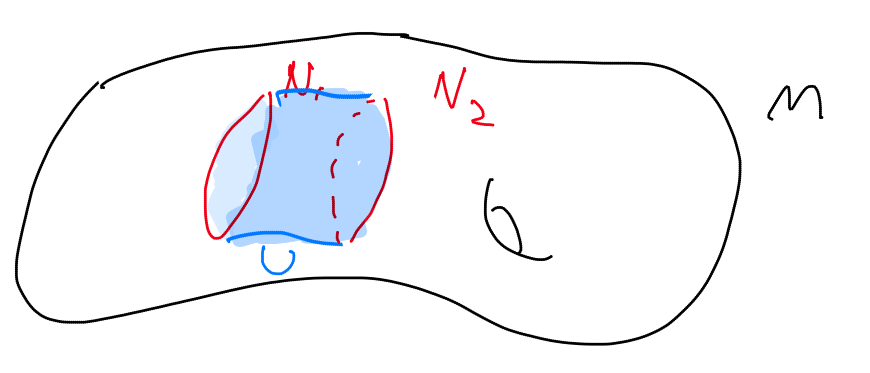
\includegraphics[width=.5\textwidth]{nearby.png}
  \caption{Two `nearby' submanifolds $N_1$ and $N_2$ within $M$.}
  \label{fig:nearby}
  \end{figure}
  
\begin{proposition}
  If the $p$-form $\omega$ satisfies $d\omega=0$,
  $\int N_1 \omega = \int N_2 \omega$ for two `nearby '$p$-dimensional  submanifolds $N_1$ and $N_2$ of $M$, 
  where $N_1$ and $N_2$ are defined to be `nearby' 
  if there is a $(p+1)$-dimensional submanifold $U$ such that $\partial U = N_1\sqcup \overline{N_2}$.
\end{proposition}
See Fig.~\ref{fig:nearby} for an illustration of the concept `nearby';
the notation $\sqcup$ is for the disjoint union,
and the overline above $N_2$ means that the orientation is reversed. 
Note that the terminology `nearby' is introduced here just for this proposition
and is not a standarad one.
A proper concept to be used here is the homology, but the definition is fairly complicated and will be postponed for a while.
The proof is extremely simple: \begin{equation}
\int_{N_1} \omega - \int_{N_2} \omega = \int_{\partial U}\omega=\int_U d\omega = 0.
\end{equation}

This motivates us the following definitions.
\begin{definition}
A $p$-form $\omega$ is called \emph{closed} when $d\omega=0$,
and is called \emph{exact} when it has the form $\omega=d\eta$ for some $(p-1)$-form $\eta$.
\end{definition}
Since $d^2=0$, we have
\begin{proposition}
An exact form is automatically closed.
\end{proposition}

We can now introduce an equivalence relation between two closed $p$-forms, 
by defining $\omega_1\sim \omega_2$ if $\omega_1-\omega_2=d\eta$ for some $(p-1)$-form $\eta$.
\begin{definition}
  The equivalence class $[\omega]$ of a closed $p$-form $\omega$ is called its \emph{cohomology class}.
  The space of all such cohomology classes  is denoted by $H^p_\text{dR}(M)$.
  This is the de Rham cohomology group of $M$.
\end{definition}
Note that although it is called a group, it is simply a vector space over $\bR$.

The preceding discussions on integrations of $p$-forms on $p$-dimensional submanifolds imply the following:
\begin{proposition}
  The integral of a cohomology class $[\omega] \in H^p_\text{dR}(M)$ 
  on a $p$-dimensional closed submanifold $N$ of $M$ is well-defined.
  Moreover, the integral of a cohomology class $[\omega]$ on two `nearby' submanifolds $N_1$ and $N_2$ is the same.
\end{proposition}

In particular, if $[\omega]$ is such that there is an $N$ with $\int_N \omega\neq 0$,
then there is no $\eta$ such that $\omega=d\eta$.
This also shows that $N$ is not the boundary of any $(p+1)$-dimensional submanifold $U$,
so $N$ is guaranteed to be `nontrivial within $M$'.

Recall that given a map $f:X\to Y$, there was a pull-back map $f^*: \Omega^p(Y)\to \Omega^p(X)$.
This induces a map $f^*: H^p_\text{dR}(Y)\to H^p_\text{dR}(X)$,
which we also call as the pull-back.
This is clearly a linear map between two vector spaces. 
From this it easily follows that:
\begin{proposition}
  If $X$ and $Y$ are diffeomorphic, $H^p_\text{dR}(X)$ and $H^p_\text{dR}(Y)$ are isomorphic.
\end{proposition}

\begin{proposition}
  For a compact $M$, $H^p_\text{dR}(M)$ is finite dimensional.
\end{proposition}
Note that the space of closed $p$-forms and exact $p$-forms are function spaces
and typically infinite dimensional. 
That their `difference' is finite dimensional is an interesting fact,
which we cannot prove here.

In contrast to homotopy, the de Rham cohomology group is computable,
in the sense that there is an algorithm to compute it,
given the description of a manifold in terms of patches,
although we can not go into the details here.
But this makes the cohomology groups a useful object when studying the topology of a manifold.

The cohomology groups have another structure.
To see this, let $\alpha$ and $\beta$ a $p$-form and a $q$-form, respectively.
When $d\alpha=0$ and $d\beta=0$, we have \begin{equation}
d(\alpha \wedge \beta)=(d\alpha)\wedge \beta + (-1)^p\alpha \wedge  d\beta =0.
\end{equation}
Also, when $\alpha=d\eta$, \begin{equation}
\alpha\wedge \beta=d(\eta\wedge \beta).
\end{equation}
This means that 
\begin{proposition}
The operation of taking two cohomology classes
$[\alpha] \in H^p_\text{dR}(M)$,
$[\beta] \in H^q_\text{dR}(M)$ 
and forming $[\alpha\wedge \beta] \in H^{p+q}_\text{dR}(M)$ gives a
well-defined bilinear multiplication \begin{equation}
H^p_\text{dR}(M) \times H^q_\text{dR}(M)
\to H^{p+q}_\text{dR}(M).
\end{equation}
\end{proposition}




\subsection{Examples of de Rham cohomology}
Let us at least  give some examples of nontrivial de Rham cohomology classes.

\begin{proposition}
$H^0_\text{dR}(M)=\bR^k$,
where $k$ is the number of connected components of $M$.
\end{proposition}
To see this, note that there is no exact $0$-form, since there is no $-1$-form to start with.
A closed $0$-form is a function $f$ such that $df= \frac{\partial f}{\partial x_i}dx_i=0$ at every point.
This means that all the partial derivatives of $f$ vanish at every point on $M$.
Therefore $f$ is locally constant,
and is specified by assigning a constant at each connected component of $M$.

\begin{example}
$H^p_\text{dR}(S^n)$ is given by \[
H^p_\text{dR}(S^n)= \begin{cases}
\bR & (p=0),\\
0 & (p=1,\ldots, n-1),\\
\bR & (p=n).
\end{cases}
\]
\end{example}

Let us start with $n=1$. Parameterize $S^1$ by $0\le \theta \le 2\pi$.
We already discussed $p=0$ above in general.
Take $p=1$, then. A one-form is $g:=g(\theta)d\theta$, and it satisfies $dg=0$ automatically.
Assume such a $g(\theta)$ is given by $df=f'(\theta) d\theta$.
This means $g(\theta)=f'(\theta)$, i.e.~$f(\theta)=c+ \int_0^\theta g(t)dt$.
$f$ is a function on a circle, and therefore $f(0)=f(2\pi)$.
This means that $g(\theta)d\theta$ is exact if and only if $\int_0^{2\pi} g(\theta)d\theta=0$.
Note that this right hand side is simply $\int_{S^1} g$.
Therefore, two one-forms $g_1$ and $g_2$ satisfy $[g_1]=[g_2]$ if and only if $\int_{S^1} g_1=\int_{S^2}g_2$.
This means $H^1_\text{dR}(S^1)=\bR$.

For general $n$ I only give a rough check of the statement.
Take a $p$-dimensional closed submanifold $N\subset S^n$
and consider  $\int_N \omega$.
When $0<p<n$,
we can always shrink $N$ within $S^n$ to find a $U\subset S^n$ such that $\partial U=N$.
Then \begin{equation}
\int_N \omega=\int_{U} d\omega=0.
\end{equation}
This is compatible with $H^p_\text{dR}(S^n)=0$ for $0<p<n-1$.
For $p=n$, the cohomology class $[\omega]$ is detected by $\int_{S^n} \omega$; 
note that $S^n$ cannot be shrunk within $S^n$, so it is OK that $\int_{S^n}\omega$ can be nonzero.


\begin{example}
$H^p_\text{dR}(\CP^n)$ is given by \[
H^p_\text{dR}(\CP^n)= \begin{cases}
\bR & (p: \text{even}), \\
0 & (p: \text{odd}) .
\end{cases}
\]
Furthermore, denoting a nontrivial element of $H^2_\text{dR}(\CP^n)$ by $c$,
$c^k \in H^{2k}_\text{dR}(\CP^n)$  is also nontrivial. 
So, as an algebra, we have \[
\bigoplus_p H^p_\text{dR}(\CP^n) = \bR[c]/(c^{n+1}).
\]
\end{example}

Consider two patches given by \begin{equation}
[1:z_2:z_3:\cdots:z_{n+1}]
\end{equation} and \begin{equation}
[w_1: 1: w_3:\cdots:w_{n+1}]
\end{equation} respectively. Recall that the coordinates are related as $w_i = z_i/z_2$, with the convention $z_1=1$ and $w_2=1$. 
There are other patches but they can be treated in the same manner.

Let us consider the 1-form $A_{(z)}$ defined on the 1st patch, given by \begin{equation}
A_{(z)} =  \frac{1}{2i} \frac{\sum_a (z_a d\bar z_a-\bar z_a dz_a)}{1+\sum_a |z_a|^2}.
\label{eq:CPnConn1}
\end{equation} 
We can consider similarly \begin{equation}
A_{(w)} =  \frac{1}{2i} \frac{\sum_a (w_a d\bar w_a-\bar w_a dw_a)}{1+\sum_a |w_a|^2}
\label{eq:CPnConn2}
\end{equation}  defined on the 2nd patch.
On the overlap of the two patches, a short computation shows that \begin{equation}
A_{(z)}=A_{(w)} + \frac{1}{2i} (\frac{dw_1}{w_1}-\frac{d\bar w_1}{\bar w_1})
=A_{(w)} + {d\theta_1},
\label{eq:CPnConn3}
\end{equation}
where we introduced $w_1=r_1 e^{i\theta_1}$.  
Therefore $A_{(z)}$ is not well defined around the locus $w_1=0$.
But the equation above also shows \begin{equation}
dA_{(z)}=dA_{(w)} \label{eq:CPzw}
\end{equation} on the overlap. 
Using this, we define the 2-form $\omega$ by $
\omega := dA_{(z)} /(2\pi)
$ on the first patch,
and $
\omega:=dA_{(w)}/(2\pi)
$ on the second patch. 
Thanks to \eqref{eq:CPzw}, $\omega$ is well-defined everywhere, and $d\omega=0$.
Explicitly, we have
\begin{equation}
\omega = \frac{1}{2\pi}\frac{1}{i} \left(
\frac{\sum_a dz_a \wedge d\bar z_a}{1+\sum_a |z_a|^2}
-\frac{(\sum_a \bar z_a dz_a) \wedge (\sum_a z_a d\bar z_a)}{(1+\sum_a |z_a|^2)^2}
\right)
\label{eq:CPnConn4}
\end{equation} on the first patch.

We are going to show that $\omega^m$ is a nontrivial cohomology class for $m=0,\ldots, n$, by integrating them on suitable $2m$-dimensional submanifolds.
Now, the subspace of $\CP^n$ given by \begin{equation}
\{ [z_1:z_2:\cdots:z_{n+1}] \mid  z_{m+2}=z_{m+3}=\cdots=z_{n+1}=0\} 
\end{equation} is  $\CP^m$.
We do the computation inductively on $m$.
For $m=1$, $\CP^1$ is simply parameterized by $z:=z_2$ alone. We need to compute \begin{equation}
\int_{\CP^1} \omega = \int \frac1{2\pi} \frac{1}{i} \frac{dz \wedge d\bar z}{(1+|z_2|^2)^2} .
\end{equation} This can be computed explicitly to be $=1$, 
but to make the inductive process clearer, we instead write it as \begin{equation}
\int_{\CP^1} \omega= \int_{z,\bar z} dA_{(z)} = \oint_{|z|=R} A_{(z)}
= \oint_{|w|=1/R} (A_{(w)} + \frac{d\theta}{2\pi}).
\end{equation} where we changed the patch from the 1st one (parameterized by $z:=z_2$)  to 
the 2nd one (parameterized by $w:=w_1$) in the last equality.
As $A_{(w)}$ is well-defined on the 2nd patch, its integral around $|w|=1/R$ vanishes in the limit $R\to \infty$, leaving only the second term, which gives \begin{equation}
= \oint \frac{d\theta_1}{2\pi} = 1.
\end{equation}

For $m>1$, the approach is analogous. 
We note $\omega^m = d(A_{(z)} \omega^{m-1})$ on the first patch.
The first patch is parameterized by $z_2$, \ldots, $z_{m+1}$,
and therefore has the topology of $\bC^m=\bR^{2m}$.
It has an asymptotic boundary $S^{2m-1}$ at infinity.
So we have \begin{equation}
\int_{\CP^m} \omega^m = \int_{\bC^m} d(A_{(z)} \omega^{m-1}) = \int_{S^{2m-1}} A_{(z)} \omega^{m-1},
\end{equation}
where the last integral is over the asymptotic boundary $S^{2m-1}$ of the first patch.

Now, the complement of the first patch within $\CP^m$ is the locus \begin{equation}
\{ [0:z_2:\cdots z_{m+1}] \in \CP^m \} \simeq \CP^{m-1}.
\end{equation}
So, the asymptotic boundary $S^{2m-1}$ is an $S^1$ fiber bundle over this $\CP^{m-1}$.
Our idea is to first perform the integral of $A_{(z)} \omega^{m-1}$ over the fiber $S^1$, and then integrate the result over $\CP^{m-1}$.

To identify the integral over $S^1$, it is useful to go to the second patch,
in which the asymptotic boundary of the first patch
is at $|w_1|=1/R$ with very small $R$.
So we have  \begin{equation}
\int_{\CP^m} \omega^m = \oint_{\{  |w_1|=1/R  \} \cap \CP^m } 
(A_{(w) } + \frac{d\theta_1}{2\pi} ) \omega^{m-1}.
\end{equation}
Now, $A_{(w)}$ is well-behaved at $w_1=0$, and therefore its integral over a small circle $|w_1|=1/R$ vanishes.
Therefore only the contribution from $d\theta_1/(2\pi)$ remains, and we have \begin{equation}
\int_{\CP^m} \omega^m = \oint \frac{d\theta_1}{2\pi} \int_{\CP^{m-1}} \omega^{m-1}
= \int_{\CP^{m-1}} \omega^{m-1}.
\end{equation}
Doing this repeatedly, we find that it is equal to $1$.



\subsection{Connection and the Maxwell field}
\label{subsec:U1connection-as-Maxwell}

We saw above that, on $M=\bR^3$, the relation between the vector potential and the magnetic field strength is given by $B=dA$,
where $A=A_x dx + A_y dy + A_z dz$ and $B=B_x dy\wedge dz + B_y dz\wedge dx + B_z dx\wedge dy$.
On a more complicated manifold, it is still true that the magnetic field $B$ is a 2-form,
but the vector potential $A$ is not quite a 1-form.

To motivate it, we start from the Hamiltonian of an electrically-charged particle of charge $q$ in a magnetic field, which is given by \begin{equation}
H = \frac{1}{2m} \sum_{a=1,2,3}\left( -i\hbar\frac{\partial}{\partial x^a} - q A^\text{SI}_a \right)^2 ,
\end{equation}
acting on a wavefunction $\psi$. 
The gauge transformation \begin{equation}
A^\text{SI}_a \mapsto \tilde A^\text{SI}_a:=A^\text{SI}_a + \frac{\partial \chi}{\partial x^a}
\end{equation} needs to be supplemented by the transformation of the wavefunction \begin{equation}
\psi \mapsto \tilde \psi = e^{iq\chi/\hbar} \psi. \label{eq:gauge-tr}
\end{equation}
Indeed, one can check that \begin{equation}
  \left( -i\hbar\frac{\partial}{\partial x^a} - q \tilde A^\text{SI}_a \right) 
  e^{iq\chi/\hbar}\psi=
  e^{iq\chi/\hbar} \left( -i\hbar\frac{\partial}{\partial x^a} - q A^\text{SI}_a \right) \psi
\end{equation}
and therefore the Hamiltonian after the gauge transformation, \begin{equation}
\tilde H= \frac{1}{2m} \sum_{a=1,2,3}\left( -i\hbar\frac{\partial}{\partial x^a} - q \tilde A^\text{SI}_a \right)^2,
\end{equation} is conjugate to the original Hamiltonian $H$: \begin{equation}
\tilde H = e^{iq\chi/\hbar} H e^{-iq\chi/\hbar},
\end{equation} and therefore the eigenvalues are unchanged. 

Now, we can identify \eqref{eq:gauge-tr} as the patching rule of a complex line bundle $L\to M$  between two patches $U$ and $V$ of $M$:
\begin{equation}
  U\times \bC \ni (b,\psi(b)) \mapsto (b,\tilde\psi(b))=(b,g(b)\psi(b)) \in V\times \bC,
\end{equation} where $g:U\cap V\to U(1)=\{|z|=1\}$, $g(b)=e^{iq\chi(b)/\hbar}$.
We now consider \begin{equation}
D\psi :=(d - i A )\psi = \sum_a \left(\frac{\partial}{\partial x^a} - i A_a\right)\psi dx^a
\end{equation} and \begin{equation}
D\tilde\psi:=(d - i\tilde A) \tilde\psi = \sum_a \left(\frac{\partial}{\partial x^a} - i \tilde A_a\right)\tilde\psi dx^a,
\end{equation} where \begin{equation}
A= \sum_a A_a dx^a, \qquad A_a := \frac{q}{\hbar} A^\text{SI}_a,
\end{equation} and similarly for the tilded version, so that \begin{equation}
\tilde A_a = A_a - i g^{-1} \frac{\partial g}{\partial x^a},
\end{equation} or equivalently \begin{equation}
\tilde A = A - i g^{-1} dg.
\end{equation}
We then find that \begin{equation}
D\tilde \psi = (d + i\tilde A) \tilde\psi = g(b) (d + i A) \psi = g(b) D\psi,
\end{equation}
meaning that $D\psi$ on the patch $U$ and $D\tilde \psi$ on the patch $V$
 combine to define a section of $(L\otimes T^*M) \to M$.

\begin{definition}
A connection on a complex line bundle $L\to M$ 
(or equivalently a principal $U(1)$ bundle $P\to M$)
is a collection of 1-forms $A_{(U)}$ on patches $U$ on $M$ such that \begin{equation}
  A_{(V)}=A_{(U)} - i g^{-1} dg
\end{equation}
on the overlap $U\cap V$, when the line bundle is built from the patching rule \begin{equation}
  U\times \bC \ni (b,\psi(b)) \mapsto (b,\tilde\psi(b))=(b,g(b)\psi(b)) \in V\times \bC,
\end{equation}
where $g:U\cap V\to U(1)$.
\end{definition}

We do not usually write the subscript $A_{(U)}$ explicitly,
and we simply refer to them as $A$.

Let $F_{(U)}=dA_{(U)}$ on each patch $U$.
Then we have \begin{equation}
F_{(V)}=dA_{(V)}=dA_{(U)} - i d(g^{-1} d g) = F_{(U)}.
\end{equation}
(To show the last equality above, 
it is useful to note that $g=e^{i\theta(b)}$ for some function $\theta(b)$
at least locally.
Then $-ig^{-1}dg = d\theta$, so $d(g^{-1}dg)=d^2\theta=0$.)
In any case, this means that $F_{(U)}$ and $F_{(V)}$ agree on the overlap $U\cap V$, and 
patch together to form a 2-form on $M$.
\begin{notation}
  Given a $U(1)$ connection $A$, 
the 2-form $F$, given locally at each patch by $F=dA$, is called the \emph{curvature} of the connection.
\end{notation}

When we studied the cohomology of $\CP^n$, we used $\omega$ defined \eqref{eq:CPnConn4},
which used one-forms $A_{(z)}$, $A_{(w)}$ defined on each patch, see  \eqref{eq:CPnConn1},  \eqref{eq:CPnConn2},  \eqref{eq:CPnConn3}.
We now recognize them as defining a $U(1)$ connection on $\CP^n$, where the patching function $g:U\cap V\to U(1)$
was given by $g = e^{i\theta_1}$.
Then the 2-form $\omega$ was  given by $\omega = F/(2\pi)$, where $F$ is the curvature 2-form.
The 2-form $\omega$ there was closed. This is general:
\begin{proposition}
The curvature 2-form is closed, $dF=0$.
\end{proposition}
This can be checked on each patch easily, $dF=d^2A=0$.
This does not mean that $F$ is always exact; for $F$ to be exact, 
we need to find a 1-form $\eta$ \emph{globally defined on $M$} 
such that $F=d\eta$.

One important feature of the curvature 2-form is the following:
\begin{proposition}
The integral of the curvature 2-form $F$ over a 2-dimensional closed submanifold $N$ of $M$ is an integer multiple of $2\pi$.
\end{proposition}
Let us show this for $N=S^2$.
We cover $S^2$ by two patches $U$ and $V$, corresponding to the northern and southern hemispheres,
so that $U$ and $V$ share a common boundary, which is the equator.
$F$ is given by $F=dA_{(U)}$ on $U$ and $F=dA_{(V)}$ on $V$.
Then we have \begin{equation}
  \int_{S^2} F = \int_{U} F+\int_V F
  = \int_{\partial U} A_{(U)} + \int_{\partial V} A_{(V)}
  = \int_{S^1} (A_{(U)}-A_{(V)})
  =\int_{S^1} -i g^{-1} dg.
\end{equation}
where $g:S^1\to U(1)$ is a map from the equator to the group $U(1)$.

We parameterize the source $S^1$ by $0\le s < 2\pi$,
and the target $U(1)$ by $z=e^{i\theta}$.
Then $g(s)=e^{i\theta(s)}$, and \begin{equation}
\int_{S^2} F = \int_0^{2\pi} \frac{d\theta}{ds} ds = 2\pi n,
\end{equation}
where $n$ is the winding number of the map $g:S^1\to U(1)$.
This integer $n$ is also known as the \emph{Chern number}.

This fact was first found by Dirac on the physics side \cite{Dirac}.
We recall that, to covert to SI, we use \begin{equation}
  F^\text{SI} = \frac{\hbar}{q} F,\qquad
  A^\text{SI} = \frac{\hbar}{q} A.
\end{equation} 
Recall also that, on $\bR^3$,
$F=B_{x}dy\wedge dz + B_{y}dz\wedge dx + B_{z}dx\wedge dy$,
and therefore the integral of $F$ over a 2-sphere $S^2$ is the magnetic flux through the sphere.
We conclude the following:
\begin{proposition}
The magnetic flux through a 2-sphere $S^2$ is quantized in units of $2\pi \hbar/e$,
where $e$ is the charge of the electron.
\end{proposition}
This is the Dirac quantization condition.

\begin{aside}
The Coulombic force between two minimally-charged electric particles, 
placed by a distance of $r$ apart, is given by \begin{equation}
  F = \frac{e^2}{4\pi \epsilon_0 r^2}.
\end{equation} 
Similarly, the Coulombic force between two minimally-charged magnetic monopoles,
placed by a distance of $r$ apart, is given by \begin{equation}
  F = \frac{g^2}{4\pi \mu_0 r^2}.
\end{equation} where $g=2\pi \hbar/e$ as discussed above.
Then we find that the ratio \begin{equation}
\frac{\text{Force between unit \emph{electric} charges at distance $r$}}
{\text{Force between unit \emph{magnetic} charges at distance $r$}}
\end{equation}
is independent of the distance $r$, and is given by 
\begin{equation}
= \frac{\mu_0}{\epsilon_0} \frac{e^4}{(2\pi \hbar)^2}
= 4 (\frac{e^2}{4\pi \epsilon_0 \hbar c })^2 \sim 0.0002\cdots,
\end{equation} 
where we used $\mu_0 \epsilon_0=1/c^2$ in the last line.
The combination within the parenthesis, \begin{equation}
\alpha = \frac{e^2}{4\pi \epsilon_0 \hbar c } \sim \frac{1}{137},
\end{equation} is known as the \emph{fine structure constant}.
\end{aside}

\begin{table}[h]
\centering
\begin{tabular}{c|c}
physics & mathematics \\
\hline
topology of Maxwell field & principal $U(1)$ bundle \\
vector potential & connection \\
field strength & curvature\\
magnetic flux  & Chern number 
\end{tabular}
\caption{Translation table of terminologies \label{tab:translation}}
\end{table}


To close this section, a  few remarks are in order:
\begin{itemize}
\item As you have seen, the same concepts are named differently in physics and mathematics. 
They are tabulated in Table~\ref{tab:translation}.
\item The curvature 2-form $F$ is closed and therefore defines an element in the de Rham cohomology group.
It has a special feature that the integral of $F/(2\pi)$ over a closed 2-dimensional submanifold is always an integer.
This motivates us to look for an analogue of de Rham cohomology defined not with $\bR$ but with $\bZ$ from the start.
This will lead us to the concept of (co)homology with coefficients in general Abelian group $A$, not just for $\bR$ and $\bZ$.
\item As this integral is an integer, the integral of $F/(2\pi)$ over various 2-dimensional submanifolds is also independent of 
continuous change of the $U(1)$-bundle and of the connection on it.
Therefore these integers give topological invariants of the $U(1)$-bundle.
This motivates us to look for a systematic way to obtain topological invariants of various other bundles.
This will lead us to the theory of characteristic classes.
\item In a 2+1 dimensional system, 
the Hall conductivity $\sigma$ is characterized by a term 
$\propto \sigma \int_M A\wedge F$ in the effective action of the system,
where $A$ is the vector potential and $F$ is the magnetic field.
This combination $\propto \int_M A\wedge F$ is known as the Chern-Simons term.
As $A$ as a 1-form is only defined on each patch, the definition of the Chern-Simons term is delicate,
which eventually leads to the quantization condition on the Hall conductivity $\sigma$ in a quantum setting,
giving an algebraic-topological explanation of the integer quantum Hall effect.
I hope to cover this  topic by the end of this lecture series!
\end{itemize}


\section{(Co)homology with $\bZ$ or $\bZ_2$ coefficients}

\subsection{Some motivations}
We saw above that there is a well-defined integral of a de Rham cohomology class $[\omega]\in H^p_\text{dR}(M)$ 
over a $p$-dimensional closed submanifold $N$ of $M$.
This was due to $\int_N d\eta=\int_{\partial N}\eta=0$.
We also saw that when $N_1$ and $N_2$ appear as the boundary of a manifold $N'$ of one higher dimension, we have \begin{equation}
\int_{N_1} \omega - \int_{N_2} \omega = \int_{N'} d\omega = 0.
\end{equation}
It is also true that $N$, $N_{1,2}$ and $N'$ do not need to be actual submanifolds;
they can all be replaced with maps $N\to M$, $N_{1,2}\to M$ and $N'\to M$, respectively,
as differential forms can be pulled back.

This means that the object on which we integrate $[\omega]\in H^p_\text{dR}(M)$ 
can be taken to be the equivalence classes of $(N, f:N\to M)$
such that two such pairs $(N_1,f_1)$ and $(N_2,f_2)$ are equivalent if they are the boundary of a pair $(N',f':N'\to M)$.
This actually is the definition of the bordism group $\Omega_p(M)$.
This is easier to compute than $\pi_p(M)$ but is still harder than $H_p(M;\bZ)$, the homology group with $\bZ$ coefficient, which we define now.

For this, we note that the manipulations we did above using $N$, $N_{1,2}$ and $N'$ 
are true not just for smooth manifolds but for polyhedra.

Take a $p$-dimensional simplex $S \subset M$.
It has $(p+1)$ faces $F_{i=1,\ldots,p+1}$, each of which is a $(p-1)$-dimensional simplex.
Then we have \begin{equation}
\int_S d\eta = \sum_{i=1}^{p+1}  \int_{F_i} \eta.
\end{equation}
Therefore, if we have a closed polyhedron $H$ consisting of many simplices $S_a$, \begin{equation}
\int_H d\eta = \sum_a \int_{S_a} d\eta = \sum_a \sum_{i=1}^{p+1}  \int_{F_{a,i}} \eta,
\end{equation}
where $F_{a,i}$ is the $i$-th face of the $a$-th simplex $S_a$.
As the same face appears with opposite orientations from two different simplices, the last sum vanishes. 

Similarly, if two closed polyhedra $H_1$ and $H_2$ appears as the boundary of 
a polyhedron $H'$ with one higher dimension, given a closed form $\omega$, we have \begin{equation}
\int_{H_1} \omega - \int_{H_2} \omega = \int_{H'} d\omega = 0.
\end{equation}
So the integral of a closed form $\omega$, or equivalently of the de Rham cohomology class $[\omega]$,
does not change when we move the polyhedron $H_1$ to $H_2$.

This suggests the following definitions.

\subsection{Singular (co)homology}

We fix an Abelian group $A$, such as $A=\bR, \bZ, \bZ_2$.
\begin{definition}
A $p$-chain $c$ with $A$ coefficient, of a topological space $M$, is a formal sum of $p$-simplices $c=\sum_a n_a S_a$,
where $n_a\in A$ and $S_a$ is a $p$-simplex (or more precisely, a map $f:S_a\to M$).
The set of all $p$-chain with $A$ coefficient is written as $C_p(M;A)$.
\end{definition}

\begin{definition}
Given a $p$-simplex $S$, the boundary $\partial S$ is a $(p-1)$-chain, given by the sum $\sum_i \pm F_i$ of its faces $F_i$, with the sign chosen appropriately.
The boundary operator $\partial:C_p(M;A)\to C_{p-1}(M;A)$ is then defined by linearity.
\end{definition}

\begin{proposition}
The boundary operator $\partial$ satisfies $\partial^2=0$.
\end{proposition}

\begin{definition}
A chain $c$ is called a cycle if $\partial c=0$.
The set of all $p$-cycles is written as $Z_p(M;A)$.
A chain $c$ is called a boundary if $c=\partial c'$ for some $(p+1)$-chain $c'$.
The set of all $p$-boundaries is written as $B_p(M;A)$.
\end{definition}

A $p$-cycle of $M$ is essentially a $p$-dimensional closed polyhedron in $M$ we discussed above. 

\begin{definition}
The singular homology group $H_p(M;A)$ is defined as the quotient \begin{equation}
H_p(M;A) = \frac{Z_p(M;A)}{B_p(M;A)} = \frac{\Ker \partial: C_p(M;A)\to C_{p-1}(M;A)}{\Im \partial: C_{p+1}(M;A)\to C_p(M;A)}.
\end{equation}
\end{definition}

The singular cohomology group is defined similarly. 
\begin{definition}
A $p$-cochain $c$ with $A$ coefficient, of a topological space $M$, is a $\bZ$-linear map $c:C_p(M;\bZ)\to A$.
\end{definition}

\begin{definition}
  Given a $p$-cochain $c$, we define its coboundary $\delta c$ as a $(p+1)$-cochain, given by \begin{equation}
    (\delta c)(a) = c(\partial a)
  \end{equation} where $a$ is a $(p+1)$-chain.
\end{definition}

\begin{definition}
A cochain $c$ is called a cocycle if $\delta c=0$.
The set of all $p$-cocycles is written as $Z^p(M;A)$.
A cochain $c$ is called a coboundary if $c=\delta c'$ for some $(p-1)$-cochain $c'$.
The set of all $p$-coboundaries is written as $B^p(M;A)$.
\end{definition}


\begin{proposition}
The coboundary operator $\delta$ satisfies $\delta^2=0$.
\end{proposition}

\begin{definition}
The singular cohomology group $H^p(M;A)$ is defined as the quotient \begin{equation}
H^p(M;A) = \frac{Z^p(M;A)}{B^p(M;A)} = \frac{\Ker \delta: C^p(M;A)\to C^{p+1}(M;A)}{\Im \delta: C^{p-1}(M;A)\to C^p(M;A)}.
\end{equation}
\end{definition}

By construction, there is a pairing between $H^p(M;A)$ and $H_p(M;A)$:
\begin{definition}
Given  $[c]\in H^p(M;A)$ and $[c']\in H_p(M;A)$
coming from a $p$-cochain $c$ and a $p$-chain $c'$,
we define their pairing as \begin{equation}
\langle [c],[c']\rangle = c(c').
\end{equation}
\end{definition}
This is the counterpart of an integral of a de Rham cohomology class on a closed manifold.

We note that, given a map $f:M\to M'$,
we have a map $f_*:C_p(M;A)\to C_p(M';A)$, 
compatible with the action of $\partial$.
Therefore we have a map $f_*: H_p(M;A)\to H_p(M';A)$.
It is fairly clear from the definition that $f_*$ only depends on the homotopy class of $f$.

We can also define a map $f^*:C^p(M';A)\to C^p(M;A)$ by \begin{equation}
(f^*c)(a) = c(f_*a),
\end{equation} which is compatible with the action of $\delta$.
Therefore we have a map $f^*: H^p(M';A)\to H^p(M;A)$.
Summarizing, we have:
\begin{proposition}
Given a map $f:M\to M'$, we have natural homomorphisms 
 $f_*: H_p(M;A)\to H_p(M';A)$ and $f^*: H^p(M';A)\to H^p(M;A)$,
 which only depends on the homotopy class of $f$.
\end{proposition}

Note that homology preserves the direction of the arrow, while cohomology reverses it.

\begin{corollary}
  $H_p(M;A)$ and $H^p(M;A)$ only depends on the homotopy equivalence class of $M$.
\end{corollary}

So singular (co)homology groups are very nice as topological invariants,
but they are not easy to compute from their definitions,
as we need to consider arbitrary formal sums $c=\sum_a n_a S_a$ of arbitrary simplices.

\subsection{Simplicial (co)homology}
We can set up a similar (co)homology theory which is easier to compute.

\begin{definition}
  \label{def:simplicial}
An abstract simplicial complex $K$ is a collection of simplices of various dimensions, such that \begin{itemize}
\item if a simplex $\sigma$ is in $K$, then all its faces are also in $K$.
\item given two simplices $\sigma_1$ and $\sigma_2$ in $K$, its intersection $\sigma_1\cap \sigma_2$ is either empty or a face of both $\sigma_1$ and $\sigma_2$. 
\end{itemize}
\end{definition}



\begin{definition}
Giving a manifold $M$ the structure of a simplicial complex $K$ is called a triangulation of $M$.
\end{definition}

\begin{proposition}
  Any smooth manifold has a triangulation.
\end{proposition}


\begin{definition}
  A simplicial $p$-chain $c$ of a simplicial complex $K$ is a formal sum of $p$-simplices $c=\sum_a n_a \sigma_a$ in $K$, where $n_a\in A$.
  The set of all simplicial $p$-chains is written as $C_p(K;A)$.
\end{definition}

The boundary operator $\partial$ is defined as before, and it satisfies $\partial^2=0$.
We can define the concept of cycles, boundaries, homology groups, cochains, coboundaries and cohomology groups as before.
The resulting (co)homology groups are called the simplicial (co)homology groups.

They are easier to compute than the singular (co)homology groups, 
as we only need to consider definite simplices in a triangulation,
not arbitrary formal sums of arbitrary simplices.
Often the number of simplicies of a triangulation is finite, and 
then all what is left is a finite-dimensional linear algebra over 
the coefficient Abelian group $A$ of your choice, $\bR, \bZ, \bZ_2$.

Unfortunately, it is not easy to define the map $f_*$ and $f^*$ 
for simplicial (co)homology groups, given a map $f:K\to K'$ 
between simplicial complexes,
because we often need to consider maps which do not preserve the simplicial structure.
What saves the day is the following remarkable theorem:
\begin{theorem}
For reasonable spaces $M$ with a structure of a simplicial complex,
there is a natural isomorphism between the singular and simplicial (co)homology groups, 
\begin{align}
  H_p^\text{singular}(M;A)&\simeq H_p^\text{simplicial}(M;A)\\
  H^p_\text{singular}(M;A)&\simeq H^p_\text{simplicial}(M;A).
\end{align}

\end{theorem}


\subsection{Cellular (co)homology}

The second condition in Definition \ref{def:simplicial} makes it somewhat hard to find a minimal triangulation of a manifold, though. 
For example, internet says that a minimal triangulation of $T^2$ requires 14 triangles.
Triangulations also only allow simplices. 
There are more flexible structures called CW complexes, which allow more general basic objects to build up spaces,
with a corresponding theory of (co)homology groups.
Here CW stands for `closure-finite and weak topology'.

\begin{definition}
  A CW complex $X$ of dimension $0$ is a collection of points.
\end{definition}

\begin{definition}
A CW complex $X$ of dimension $n$ is a topological space obtained by 
gluing $n$-dimensional cells $e_i$ indexed by $i$, 
i.e.~copies of $D^n$
to a CW complex $X'$ of dimension $(n-1)$ by 
attaching maps $f_i:\partial e_i = S^{n-1}\to X'$.
\end{definition}

\begin{example}
$S^n$ can be built up by attaching a single $n$-cell to a point.
\end{example}

Consider $\CP^n$, parameterized by $[x_1:\cdots:x_{n+1}]$.
The subspace $x_1=0$ is $\CP^{n-1}$.
$\CP^n \setminus \CP^{n-1}$ is parameterized by $[1:x_2:\cdots:x_{n+1}]$,
which is a copy of $\bC^n\simeq \bR^{2n}$.
Topologically, we can replace it with $B^{2n}$, 
with the attaching map $\partial B^{2n}=S^{2n-1}\to \CP^{n-1}$ given by 
the fibration $S^{2n-1}\to \CP^{n-1}$.
Doing this recursively, we find:
\begin{example}
$\CP^n$ has a structure of a CW complex with one $0$-cell, 
one $2$-cell, \ldots, one $2n$-cell.
\end{example}

We can now define a cellular (co)homology theory.

\begin{definition}
Given a CW complex $X$,
a cellular $p$-chain $c$ is a formal sum of $p$-cells $c=\sum_a n_a e_a$ in $X$, where $n_a\in A$.
\end{definition}

Compared to singular / simplicial cases, the definition of the boundary map is a bit trickier. 
\begin{definition}
Given a $p$-cell $e$ of $X$, $\partial e$ is defined to be \begin{equation}
\partial e = \sum_{e'} n(e,e') e'
\end{equation} where $e'$ runs over all $(p-1)$-cells, and $n(e,e')$ is 
the winding number of the following composition of maps: \begin{equation}
S^{p-1}\simeq  \partial e \xrightarrow{f_e} X_{p-1} \to X_{p-1}/(X_{p-1}\setminus e') \simeq S^{p-1}
\end{equation}
where $f_e$ is the attaching map of $e$.
\end{definition}

\begin{proposition}
The boundary operator $\partial$ satisfies $\partial^2=0$.
\end{proposition}

We can then define the concepts of cycles, boundaries, homology groups, cochains, coboundaries and cohomology groups as before.
We now have a remarkable fact:

\begin{theorem}
  For reasonable spaces $M$ with a structure of a CW complex,
  singular, simplicial and cellular (co)homology groups are isomorphic.
\end{theorem}

We also have

\begin{theorem}
The de Rham cohomology of a smooth manifold $M$
is isomorphic to the singular/simplicial/cellular 
cohomology of $M$ with $\bR$ coefficient, i.e. \begin{equation}
H^p_\text{dR}(M)\simeq H^p(M;\bR).
\end{equation}
\end{theorem}

Summarizing,
singular (co)homology groups are difficult to compute but their topological properties are easier to establish.
Simplicial and cellular cohomology groups are can be computed algorithmically,
 but their topological properties are harder to establish.
They agree in any case, so we are in quite a good shape.

For example, it is now very easy to prove the following:
\begin{corollary}
  The (co)homology groups $H^p(M;A)$ and $H_p(M;A)$ of a reasonable space of dimension $n$ can be nonzero
  only for $0\le p\le n$.
\end{corollary}
This is because we can only have $p$-cells for $0\le p\le n$. Done.


Simplicial/cellular complex also allows us to define the fundamental class of 
a connected $n$-dimensional manifold $M$ in an intuitive way.
Let us take a CW complex $M$.
\begin{definition}
If an $n$-chain $c=\sum_{\sigma} \pm \sigma$,
where $\sigma$ runs over all the $n$-dimensional cells of $M$, is such that $\partial c=0$,
then the homology class $[c]$ is called the fundamental class of $M$
and is denoted by $[M]$.
When such a chain with coefficients in $A$ exists, 
we say that $M$ is $A$-orientable.
\end{definition}

A more general but equivalent definition of the orientability is:
\begin{definition}
  A connected space $M$ is called $A$-orientable if $H_n(M;A)\simeq A$.
  In such a case, the homology class  corresponding to $1\in A$ 
  is called the fundamental class of $M$ and is written as $[M]$.
\end{definition}
The fundamental class $[M]$ is the homology class of the whole space $M$
as a polyhedron.

Let us also give an outline of an important fact known as the Poincar\'e duality:
\begin{theorem}
  When a smooth compact $n$-dimensional manifold $M$ is $A$-orientable,
  we have a natural isomorphism $H_p(M;A)\simeq H^{n-p}(M;A)$.
\end{theorem}

  
\begin{proof}
  We take a triangulation of $M$.
  It has $p$-dimensional simplices for $p=0,\ldots,n$.
  We now take a \emph{dual} cell decomposition of $M$:
  we put zero cells at the `barycenters' of the $n$-simplices,
  one cells at the barycenters of the $(n-1)$-simplices, and so on.
  In this manner, the simplicial chain groups $C_p(M;A)$ 
  and the cellular cochain groups $C^p(M;A)$ are isomorphic on the nose.
  With the extra assumption of the $A$-orientability,
  we can show that the action of $\partial$ and $\delta$ are also the same.
  Therefore we have $H_p(M;A)\simeq H^{n-p}(M;A)$.
\end{proof}

Again the proof becomes much easier with the simplicial/cellular complex.

Another application of a fundamental class is the following.
Suppose we have a smooth $p$-dimensional submanifold $N$ of $M$,
or more generally a smooth map $f:N\to M$.
Assume $N$ is $A$-orientable.
Then we can take the fundamental class $[N]\in H_p(N;A)$ of $N$,
and send it via $f_*$ to $f_*([N])\in H_p(M;A)$.
A natural question then arises: are all homology classes in $M$ of this form?
Are there any degree-$p$ homology classes in $M$ which does not come 
from a $p$-dimensional manifold?
This was posed by Steenrod, and the way to answer it was found by Thom
by introducing the concept of cobordism;
indeed there are homology classes which do not come from manifolds
and can only be given by a closed polyhedron.
We will come back to this question later.

\subsection{Examples}
Let us move on to examples. 
Cellular (co)homology allows us to compute the (co)homology groups of $S^n$ and $\CP^n$ very easily, 
because there are so few cells in their CW complexes.

\begin{example}
The (co)homology groups of $S^n$ are given by \begin{align}
H_p(S^n;A) &= \begin{cases} A & p=0,n \\ 0 & \text{otherwise} \end{cases}, \\
H^p(S^n;A) &= \begin{cases} A & p=0,n \\ 0 & \text{otherwise} \end{cases}.
\end{align}
\end{example}
This is very easy except for $n=1$, since there are only cells at dimension $n$ and $0$,
and the boundary maps are forced to be trivial.

\begin{example}
  \label{ex:cohoCPn}
The (co)homology groups of $\CP^n$ are given by \begin{align}
H_p(\CP^n;A) &= \begin{cases} A & p=0,2,4,\ldots,2n \\ 0 & \text{otherwise} \end{cases}, \\
H^p(\CP^n;A) &= \begin{cases} A & p=0,2,4,\ldots,2n \\ 0 & \text{otherwise} \end{cases}.
\end{align}
\end{example}
This is also very easy, since there are only even-dimensional cells,
and the boundary maps are just zero.

The (co)homology group of $\RP^n$ is slightly trickier to compute,
since it has cells in every dimension.
Recall that $\RP^n$ is parameterized by $[x_1:\cdots:x_{n+1}]$,
and the subspace $\RP^{n-1}$ is given by $x_1=0$.
Its complement is parameterized by $[1:x_2:\cdots:x_{n+1}]$,
which is a copy of $\bR^n$.
Topologically, we have $B^n$ with the attaching map $\partial B^n=S^{n-1}\to \RP^{n-1}$, 
which is the 2:1 map we repeatedly discussed.
So we have a single cell $e^i$ at dimension $i$ for each $i$.
The boundary map can be found by examining \begin{equation}
\partial B^n = S^{n-1} \xrightarrow{2:1} \RP^{n-1} \to \RP^{n-1}/\RP^{n-2} \simeq S^{n-1}.
\end{equation}
This has the degree $2$ if $n$ is even, and $0$ if $n$ is odd.
The chain groups and cochain groups are both given by $C_p(\RP^n;A)=A$ 
and $C^p(\RP^n;A)=A$ for all $0\le p\ge n$, with the (co)boundary maps given as 
\begin{equation}
C_0 \xleftarrow{0} C_1 \xleftarrow{2} C_2 \xleftarrow{0} C_3 \xleftarrow{2} C_4 \cdots
\end{equation}
and 
\begin{equation}
C^0 \xrightarrow{0} C^1 \xrightarrow{2} C^2 \xrightarrow{0} C^3 \xrightarrow{2} C^4 \cdots
\end{equation}
respectively. 
From this we see 
\begin{example}
The (co)homology groups of $\RP^n$ with $\bZ_2$ coefficient are given by \begin{equation}
H_p(\RP^n;\bZ_2) = \bZ_2,\qquad
H^p(\RP^n;\bZ_2) = \bZ_2
\end{equation} for all $0\le p\le n$, while \begin{equation}
\begin{array}{c|ccccccccccccccccc}
  p& 0 &  1 & 2 & 3 & 4 & 5 & \cdots \\
  \hline
  H_p(\RP^n;\bZ) & \bZ & \bZ_2  & 0 & \bZ_2&  0 & \bZ_2 & \cdots \\
  H_p(\RP^n;\bR) & \bR & 0 & 0 & 0 & 0 & 0 & \cdots \\
  H^p(\RP^n;\bZ) & \bZ & 0 & \bZ_2  & 0 & \bZ_2&    0 & \cdots \\
  H^p(\RP^n;\bR) & \bR & 0 & 0 & 0 & 0 & 0 & \cdots 
\end{array} .
\end{equation}
\end{example}

Note that $\RP^n$ is always $\bZ_2$-orientable,
but $\bZ$- and $\bR$-orientable if and only if $n$ is odd.

\begin{question}
Let $\bZ_k$ acts on $\bC^n$ by \begin{equation}
   (z_1,\ldots,z_n) \mapsto e^{2\pi i/k}(z_1,\ldots,z_n).
\end{equation} 
This gives an action of $\bZ_k$ on the unit sphere $S^{2n-1}\subset \bC^n$.
Find a cell decomposition of the quotient space $S^{2n-1}/\bZ_k$,
and compute the (co)homology groups, with coefficients $A=\bR$, $\bZ$, $\bZ_k$.
\end{question}
Hint: one cell in each dimension suffices. 
Also, the answer can be found online; this space $S^{2n-1}/\bZ_k$ is known as a lens space.

\begin{question}
Let $\Sigma_g$ be an oriented compact 2-dimensional surface of genus $g$.
Show that the (co)homology groups of $\Sigma_g$ are given by \begin{equation}
H_p(\Sigma_g;A) = \begin{cases} 
  A & p=0, \\ 
  A^{2g} & p=1, \\
  A & p=2, \\
\end{cases}\qquad
H^p(\Sigma_g;A) =\begin{cases} 
  A & p=0, \\ 
  A^{2g} & p=1, \\
  A & p=2. \\
\end{cases}
\end{equation}
\end{question}

\subsection{Relation to Kitaev's toric code}

Let $A=\{0,1\}=\bZ_2$ and take a two-dimensional cell complex $M$,
consisting of vertices $v$, edges $e$ and faces $f$.
For simplicity assume that each face $f$ is a polygon with edges $e_1,\ldots,e_{n_f}$.
Introduce a qubit $\bC^2$ per edge $e$.
The Hilbert space of the system has the basis $\ket{\{m_e\}}$ where $m_e=0,1$.
So the basis of the Hilbert space is indexed by an element $m=\{m_e\}\in C^1(M;\bZ_2)$.

For each $f$, we add a local term in the Hamiltonian, 
given by 
\begin{equation}
  A_f=-\prod_{e: \text{edges of}\ f} (\sigma_z)_e.
\end{equation}
Note that 
\begin{equation}
A_f \ket{m} = \begin{cases}
  -\ket{m} & \text{if}\ (\delta m)(f)=0,\\
  +\ket{m} & \text{if}\ (\delta m)(f)=1.
\end{cases}
\end{equation}
Therefore, it gives penalties to basis elements such that $\delta m\neq 0$.
By taking the coefficient very large, we can make the ground state of the system to be the one with $\delta m=0$.

For each vertex $v$, we also add a local term in the Hamiltonian,
given by 
\begin{equation}
  B_v=-\prod_{e: \text{edges attached to}\ v} (\sigma_x)_e.
\end{equation}
Denote by $c_v\in C^0(M;\bZ_2)$ 
a cochain which is 1 at the vertex $v$ and 0 otherwise.
$\{c_v\}_v$ is a basis of $C^0(M;\bZ_2)$.
A short reflection shows that \begin{equation}
B_v \ket{m} = \ket{m+\delta c_v}.
\end{equation}
Therefore, by taking the coefficient of $B_v$ in the Hamiltonian very large,
the dynamics of the system averages over the orbit of the action $m\mapsto m+\delta c_v$,
dynamically realizing the quotient via $\delta$ applied to $C^o(M;\bZ_2)$.

Therefore we see that the ground state of the system has a basis indexed by the cohomology group $H^1(M;\bZ_2)=\bZ^{2g}$,
thus encoding $g$ logical qubits.

As good observables, take a 1-cycle $C$ in $M$.
The pairing of a cochain $m$ with $C$ is given by \begin{equation}
\langle m,C\rangle = \sum_{e\in C} m(e).
\end{equation} Multiplicatively, we have \begin{equation}
W_C:= (-1)^{\langle m,C\rangle} = \prod_{e\in C} (-1)^{m(e)} = \prod_{e \in C} (\sigma_z)_e.
\end{equation}
On the ground state of the system, $W_C$ only depends on the homology class $[C]\in H_1(M;\bZ_2)$,
which has a natural pairing with the ground states,
which are in turn indexed by the cohomology classes in  $H^1(M;\bZ_2)$.

\subsection{Product}

In the case of de Rham cohomology, 
given $[\omega]\in H^p_\text{dR}(M)$ and $[\eta]\in H^q_\text{dR}(M)$ coming from
closed differential forms $\omega$ and $\eta$,
we can define their product $[\omega][\eta] := [\omega \wedge \eta]\in H^{p+q}_\text{dR}(M)$.
As $\omega\wedge \eta=(-1)^{pq}\eta\wedge\omega$,
the product of the cohomology classes also satisfied 
$[\omega] [\eta]=(-1)^{pq}[\eta] [\omega]$.
This was the graded commutativity of the de Rham cohomology groups.

An analogous product can be defined for simplicial (co)homology groups, when the coefficient Abelian group $A$ has a product,
 which is true for $A=\bZ,\bR,\bZ_2$ we have been discussing.

For this, we regard a  $p$-cochain $c$, which is a $A$-linear map $c:C_p(M;A)\to A$,
as $A$-valued functions \begin{equation}
c(v_0,\ldots,v_p) = \pm c([v_0,\ldots,v_p]) 
\end{equation}
if $(v_0,\ldots,v_p)$ is a reordering of the vertices of a $p$-simplex in $M$,
and zero otherwise.
We note that in this notation \begin{equation}
(\delta c)(v_0,\ldots,v_{p+1})= \sum_{i=0}^{p+1} (-1)^i c(v_0,\ldots,\widehat{v_i},\ldots,v_{p+1}),\label{eq:coboundary}
\end{equation} 
where $\widehat{v_i}$ means that $v_i$ is omitted from the argument of the function $c$.

\begin{definition}
The product of a $p$-cochain $c$ and a $q$-cochain $d$ as a $(p+q)$-cochain $c\cup d$ by \begin{equation}
(c\cup d)(v_0,\ldots,v_{p+q}) = c(v_0,\ldots,v_p) d(v_p,\ldots,v_{p+q}).
\end{equation}
\end{definition}

\begin{proposition}
We have $\delta(c\cup d) = (\delta c)\cup d + (-1)^p c\cup (\delta d)$.
\end{proposition}
The proof easily follows from the  form of the coboundary operator $\delta$ given in \eqref{eq:coboundary}.

As a result, we have
\begin{proposition}
The product of the cohomology classes $[c]\in H^p(M;A)$ and $[d]\in H^q(M;A)$,
given by $[c]\cup [d] = [c\cup d]\in H^{p+q}(M;A)$,
is well-defined.
\end{proposition}

This product is graded commutative as in the case of de Rham cohomology groups,
but the proof is slightly trickier.
In the de Rham cohomology case,
the graded commutativity was due to the fact that the wedge product of differential forms is graded commutative,
$\omega\wedge\eta=(-1)^{pq}\eta\wedge\omega$.
In simplicial cohomology,
$\omega \cup \eta \neq (-1)^{pq} \eta \cup \omega$ in general,
but satisfies a more complicated relation \cite{SteenrodHigherProduct}:
\begin{definition}
The $\cup_1$ product of a $p$-cochain $c$ and a $q$-cochain $d$ is 
a $(p+q-1)$-cochain
defined by \begin{equation}
(c\cup_1 d)(v_0,\ldots,v_{p+q-1}) = \sum_{i=0}^{p-1} (-1)^{(p-i)(q+1)}c(v_0,\ldots,v_i,v_{i+q},\ldots,v_{p+q-1}) d(v_i,\ldots,v_{i+q}).
\end{equation}
\end{definition}
Then we have 
\begin{proposition}
For $p$-cochain $c$ and $q$-cochain $d$, we have \begin{equation}
c\cup d-(-1)^{pq}d\cup c = \delta(c\cup_1 d) .
\end{equation}
\end{proposition}
As a result, we have 
\begin{corollary}
The product of the cohomology classes $[c]\in H^p(M;A)$ and $[d]\in H^q(M;A)$
satisfies $[c]\cup [d] = (-1)^{pq}[d]\cup [c]$.
\end{corollary}

Under this product, the generators of cohomology groups $H^{2k}(\CP^n;\bZ)=\bZ$
given in Example~\ref{ex:cohoCPn}
is known to be $c^k$, where $c$ is the generator of $H^2(\CP^n;\bZ)=\bZ$.

\begin{aside}
As an application of the product structure in cohomology groups,
let us give another definition of the Hopf invariant
of a map $f:S^{2n-1}\to S^n$.
Recall  that $H^n(S^n;\bZ)=\bZ$.
whose generator $[\omega]$ can be thought of the volume form with coefficient in $\bZ$.
Pick a specific cochain $\omega\in Z^n(S^n;\bZ)$,
and pull it back via $f$ to get an $n$-cochain $\omega'= f^*(\omega)\in Z^n(S^{2n-1};\bZ)$.
As $H^n(S^{2n-1};\bZ)=0$, this cochain is a coboundary, $\omega'=\delta c$ for some $(n-1)$-cochain $c$.
Then we define the Hopf invariant of $f$ as \begin{equation}
  \text{Hopf}(f) = \langle c\cup \delta c,[S^{2n-1}]   \rangle \in \bZ,\label{eq:hopf-via-coho}
\end{equation}
where $\langle \cdot,\cdot\rangle$ is the pairing between homology and cohomology groups, i.e.~the integral of a cochain over a cycle.

Note that the same construction can be done via differential forms.
Indeed, take $\omega$ to be a volume form of $S^n$, satisfying $\int_{S^n}\omega=1$.
Its pull-back $f^*(\omega)$ is exact, since $H^n_\text{dR}(S^{2n-1})=H^n(S^{2n-1};\bR)=0$.
Therefore there is a $(n-1)$-form $\eta$ such that $f^*(\omega)=d\eta$.
Then the Hopf invariant is given by \begin{equation}
  \text{Hopf}(f) = \int_{S^{2n-1}} \eta\wedge d\eta.
\end{equation}
It is however not easy to see that this is actually an integer
from this description using differential forms.
\end{aside}

\begin{question}
  Show that the expression \eqref{eq:hopf-via-coho} is well-defined, i.e.~independent of the choice of $\omega$
  representing $[\omega]$ and the choice of $c$ solving $\omega'=\delta c$.
\end{question}
\begin{question}
  Show that the Hopf invariant \eqref{eq:hopf-via-coho} is zero when $n$ is odd.
\end{question}

\subsection{Universal coefficient theorem}

So far we have defined $H_p(M;A)$ and $H^p(M;A)$ for Abelian groups $A$.
In fact it is known that all of them can be obtained from $H_p(M;\bZ)$.
These are known as universal coefficient theorems.
\begin{theorem}
For the cohomology groups, we have the short exact sequence \begin{equation}
0\to \Ext(H_{p-1}(M;\bZ),A) \to H^p(M;A) \to \Hom(H_p(M;\bZ),A) \to 0,
\end{equation} and for the homology groups, we have the short exact sequence
\begin{equation}
  0\to H_p(M;\bZ)\otimes_\bZ A \to H_p(M;A) \to \Tor(H_{p-1}(M;\bZ),A) \to 0,
\end{equation}
both of which split non-canonically.
\end{theorem}
Here, 
\begin{itemize}
\item $\Hom(A,B)$ are the homomorphisms from $A$ to $B$,
\item $A\otimes_\bZ B$ is the tensor product of $A$ and $B$ over $\bZ$,
i.e.~the Abelian group generated by $a\otimes b$ for $a\in A$ and $b\in B$
where $\otimes$ is bilinear over $\bZ$,
\item $\Tor(A,B)=\text{torsion}(A)\otimes_\bZ \text{torsion}(B)$, and 
\item $\Ext(A,B)=\text{torsion}(A)\otimes_\bZ B$,
\end{itemize}
More explicitly, we always have the following structure \begin{align}
  H_p(M;\bZ) &= \bZ^{b_p} \oplus \bZ_{k_{p}} \oplus \bZ_{k_{p}'}\oplus \cdots,\\
H_p(M;\bZ_2)&= (\bZ_2)^{b_p}\oplus \bZ_{\gcd(2,k_{p})}\oplus \bZ_{\gcd(2,k_{p}')} \oplus \cdots\\
& \qquad \qquad \oplus \bZ_{\gcd(2,k_{p-1})}\oplus \bZ_{\gcd(2,k_{p-1}')} \oplus \cdots ,\\
H^p(M;\bR)&= \bR^{b_p},
\end{align} and \begin{align}
  H^p(M;\bZ)&= \bZ^{b_p} \oplus \bZ_{k_{p-1}}\oplus \bZ'_{k_{p-1}} \oplus \cdots,\\
H^p(M;\bZ_2)&= (\bZ_2)^{b_p}\oplus \bZ_{\gcd(2,k_{p})}\oplus \bZ_{\gcd(2,k_{p}')} \oplus \cdots\\
&\qquad \qquad \oplus \bZ_{\gcd(2,k_{p-1})}\oplus \bZ_{\gcd(2,k_{p-1}')} \oplus\cdots, \\
H^p(M;\bR)&= \bR^{b_p},
\end{align}
where $b_p$ and $k_p$, $k_p'$, \ldots are defined by the decomposition 
of $H_p(M;\bZ)$ in the first line above.

\begin{question}
Check this in the case of $\RP^n$.
\end{question}

When $M$ is a compact oriented connected $n$-dimensional manifold,
we already said that 
\begin{equation}
  H_p(M;\bZ)\simeq H^{n-p}(M;\bZ); \label{eq:pd}
\end{equation}
this is the Poincar\'e duality.
We also learned sometime ago that there is a natural bilinear pairing 
\begin{equation}
H^p(M;\bZ)\times H_p(M;\bZ) \to \bZ,
\end{equation}
corresponding to the integration of a $p$-form on a $p$-dimensional closed submanifold.

The universal coefficient theorem above says that
this is actually a perfect pairing between the free parts (the $\bZ^{b_p}$ part) of $H^p(M;\bZ)$ and $H_p(M;\bZ)$,
meaning that the image of the pairing is the entirety of $\bZ$.
Combining the Poincar\'e duality and the universal coefficient theorem,
we have $b_p=b_{n-p}$.
\begin{definition}
  The numbers $b_p$ are called the Betti numbers of $M$.
\end{definition}

We finally note that the Poincar\'e duality has the following consequence:
\begin{proposition}
  Let $[N]\in H_p(M;\bZ)$ 
  be a degree-$p$ homology class and $[\omega]\in H^{n-p}(M;\bZ)$ 
  be the cohomology class corresponding to it via Poincar\'e duality.
  Then, for an arbitrary class $[\eta]\in H^p(M;\bZ)$,
  we have \begin{equation}
    \langle [\eta],[N]\rangle = \langle [\eta]\cup [\omega],[M]\rangle.
  \end{equation}  
\end{proposition}

\subsection{Hurewicz theorem}

Before concluding this introductory section on (co)homology groups,
let us mention the Hurewicz homomorphisms and the Hurewicz theorem.

Let $f:S^n\to M$. This allows us to send the generator $[S^n] \in H^n(S^n;\bZ)=\bZ$ to $f^*([M])\in H^n(M;\bZ)$.
As $f^*$ only depends on the homotopy class of the map $f$, 
we found that this defines a homomorphism \begin{equation}
  h:\pi_n(M;\bZ)\to H_n(M;\bZ).
\end{equation}
This is the Hurewicz homomorphism.
Suppose $M$ is connected. Then 
\begin{theorem}
  The Hurewicz homomorphism $h:\pi_1(M;\bZ)\to H_1(M;\bZ)$ is given by the Abelianization.
\end{theorem}
Note that $\pi_1(M)$ can be a non-Abelian group,
while $H_1(M;\bZ)$ is an Abelian group.
Therefore there is no way that they can always be equal.
The theorem above says that the relation is the simplest one imaginable.

\begin{theorem}
  Suppose $M$ is connected and simply connected,
  i.e.~$\pi_0(M)=\pi_1(M)=0$.
  Suppose further that $\pi_k(M)=0$ for $k<n$.
  Then the Hurewicz homomorphism $\pi_n(M;\bZ)\to H_n(M;\bZ)$ is an isomorphism.
\end{theorem}

For example, take $M=\CP^n$.
We already computed $\pi_k(\CP^n)$ using the long exact sequence of homotopy groups of the fibration $S^1\to S^{2n+1}\to \CP^n$,
and we know $\pi_{0}(\CP^n)=\pi_1(\CP^1)=0$ and $\pi_2(\CP^2)=\bZ$.
Therefore the Hurewicz homomorphism $\pi_2(\CP^2;\bZ)\to H_2(\CP^2;\bZ)=\bZ$ is an isomorphism.
Indeed, the generator of $H_2(\CP^2;\bZ)$ is the submanifold $\CP^1\subset \CP^2$,
and is the image of a sphere $S^2\simeq \CP^1$.


As another example, consider $S^3\simeq SU(2)$.
We have a $2:1$ map $SU(2)\to SO(3)$.
$SO(3)$ has a finite subgroup $\Gamma$, which is the symmetry group of a regular icosahedron.
Let $\hat\Gamma$ denote its inverse image in $SU(2)$.
$\hat \Gamma$ is known as the binary icosahedral group.
$\hat\Gamma\subset SU(2)$ is a finite subgroup,
and therefore $S^3/\hat\Gamma$ is a compact $3$-manifold.
We already computed that $\pi_1(S^3/\hat\Gamma)=\hat\Gamma$.
What is the homology group of $M:=S^3/\hat\Gamma$?
As it is connected and oriented, $H_0(M;\bZ)=H_3(M;\bZ)=\bZ$.
By Hurewicz, $H_1(M;\bZ)$ is the Abelianization of $\hat\Gamma$,
which is known to be trivial. 
Therefore $H_1(M;\bZ)=0$.
From the universal coefficient theorem, it then follows that $H^1(M;\bZ)=0$,
from which we have $H_2(M;\bZ)=0$ via the Poinca\'e duality.
Summarizing, we found 
\begin{example}
  The homology groups of $S^3/\hat\Gamma$ are given by \begin{equation}
    H_p(S^3/\hat\Gamma;\bZ) = \begin{cases} \bZ & p=0,3 \\ 0 & \text{otherwise} \end{cases}
  \end{equation}
  and is the same as those of $S^3$.
\end{example}
This means that there are manifolds other than $S^3$ which have the same homology groups as $S^3$.
Such manifolds are called homology spheres;
the one constructed above was the first one and was discovered by Poincar\'e.

We can ask an analgous question by replacing the homology group by the homotopy group: 
is there a compact connected 3-dimensional manifold $M$ other than $S^3$ which has $\pi_1(M)=0$?
The absence of such manifolds is the famous Poincar\'e conjecture, 
which was proved by Perelman only in the 21st century.

\section{Characteristic classes}

Now that we have learned the basics of (co)homology groups with coefficients in $\bZ_2$ and/or $\bZ$,
let us see how they arise in the study of principal $G$-bundles or vector bundles.
The cohomology classes associated to bundles are called characteristic classes.

\subsection{\v Cech cohomology}

Characteristic classes we deal with below are usually constructed within the framework of \v Cech cohomology, 
which we have not introduced yet.
Due to the time constraints, we only outline the idea. 

Let $M$ be a space, and pick a `fine enough' cover $\{U_i\}$ of $M$,
so that all nonempty intersections $U_{i_1} \cap U_{i_2} \cap \cdots \cap U_{i_k}$ is contractible.
We then associate the following simplicial complex:
\begin{itemize}
\item    a vertex $v_i$ for each $U_i$,
\item an edge $E(v_i,v_j)$ for each nonempty intersection $U_{ij}=U_i\cap U_j$,
\item a triangle $T(v_i,v_j,v_k)$ for each nonempty intersection $U_{ijk}=U_i \cap U_j \cap U_k$,
\end{itemize}
and so on. 
\begin{definition}
The simplicial complex associated to an open cover is called the \emph{nerve} of the cover.
\end{definition}

\begin{definition}
The \v Cech cohomology of a space $M$ is the simplicial cohomology 
of the nerve of a `fine enough' cover of $M$.
\end{definition}

A \v Cech $p$-cochain $c$ with $A$ coefficient, associated for a cover $\{U_i\}$,
 is then  simply the set of elements \begin{equation}
 c(i_0,i_1,\cdots, i_p)
\end{equation}
antisymmetric under the interchange of $i_0,\ldots,i_p$,
and the coboundary $\delta$ is given as before by \begin{equation}
(\delta c)(i_0,\cdots, i_{p+1})=\sum_{k=0}^{p+1}(-1)^k c(i_0,\ldots,\widehat{ i_k},\ldots, i_{p+1}).
\end{equation}
It would be useful to have explicit formulas: \begin{align}
(\delta a)(i,j) &= a(i) - a(j),\\
(\delta b)(i,j,k) &= b(j,k) -b(i,k) + b(i,j) = b(i,j) + b(j,k)+ b(k,i),\\
(\delta c)(i,j,k,l) &= c(j,k,l) - c(i,k,l) + c(i,j,l) - c(i,j,k).
\end{align}

\subsection{Characteristic classes in $H^1(M;A)$}

\subsubsection{Discrete Berry phase}
We start with characteristic classes of degree $p=1$.
Let $A$ be a finite abelian group, say $A=\bZ_2$.
Consider a principal $A$-bundle $A\to P\to M$ over $M$.
Take a fine enough patch.
It is specified by patching $U_i\times A$ and $U_j\times A$ over $U_{ij}$ by a map $g_{ij}:U_{ij}\to A$, via \begin{equation}
   U_i\times A\ni (x,a) \mapsto (x,g_{ij}(x)+a)\in U_j\times A.
\end{equation} 
As $A$ is finite, $g_{ij}(x)$ is simply a constant, which we denote by $g_{ij}$.
Over a triple intersection $U_{ijk}$, let us
go from $U_i$ to $U_j$, $U_j$ to $U_k$, and $U_k$ to $U_i$. This effects
\begin{equation}
(x,a) \mapsto (x,g_{ij}a)\mapsto (x,g_{ij}g_{jk}a)\mapsto (x,g_{ij} g_{jk}g_{ki}a),
\end{equation} and therefore we have \begin{equation}
  g_{ij}g_{jk}g_{ki}=1.
\end{equation}
This means that the $g_{ij}$'s form a \v Cech 1-cochain, and therefore a cohomology class $[g] \in H^1(M;A)$.
(Note that we used multiplicative notations for the group operation here.)

Let us consider another principal $A$-bundle $A\to \tilde P\to M$ over $M$,
specified by $\tilde g_{ij}\in A$.
The bundles $P$ and $\tilde P$ are equivalent when we can find a map
\begin{equation}
  U_i\times A \ni (x,a) \mapsto (x,f_i a)\in U_i\times A
\end{equation}
such that $f_i g_{ij}= \tilde g_{ij} f_j$.
This is equivalent to \begin{equation}
\tilde g_{ij} = g_{ij} f_i f_j^{-1}, 
\end{equation} or as a \v Cech 1-cochain, \begin{equation}
\tilde g = g + \delta f
\end{equation} (where we switched to additive notation for the group operation).
Therefore the cohomology classes are the same: $[g]=[\tilde g]$.

The consideration above also shows that for any $[g]\in H^1(M;A)$,
the corresponding cochain $g_{ij}$ defines a principal $A$-bundle over $M$.
Summarizing:
\begin{proposition}
  The cohomology class $\in H^1(M;A)$ is in one-to-one correspondence with the isomorphism classes of principal $A$-bundles over $M$.
\end{proposition}

\begin{remark}
A principal $A$-bundle being trivial is therefore equivalent to the corresponding $[g]\in H^1(M;A)$ being zero.
In this sense, $[g]$ is called the \emph{obstruction} of the bundle to be trivial.
\end{remark}

A 1-cycle $C$ on $M$ is a closed path on $M$.
In the \v Cech setting, it is a sequence of edges
$i_1 \to i_2 \to \cdots \to i_{n+1}=i_1$.
The pairing between $[g]\in H^1(M;A)$ and $C$ is given by \begin{equation}
  \langle [g],C\rangle = \sum_{k=1}^{n} g_{i_k i_{k+1}}
\end{equation} (written additively),
and is the total effect of the $A$ transformation when you go around the cycle $C$.
This can be called a discrete Berry phase (for a cond-mat person),
a discrete Wilson line (for a hep-th person),
and a holonomy (for a math person).

\subsubsection{First Stiefel-Whitney class}


A characteristic class in $H^1(M;\bZ_2)$ can be defined for an $O(n)$-bundle
$O(n)\to P\to M$  too.
For this, note that $\det: O(n)\to \bZ_2$ is a homomorphism.
Using this, we can construct a principal $\bZ_2$ bundle  $\bZ_2\to \det(P)\to M$,
and then we can form the corresponding cohomology class $[g]\in H^1(M;\bZ_2)$.
\begin{definition}
  This cohomology class is denoted by $w_1(P)$, and is called the first Stiefel-Whitney class of $P$.
\end{definition}

If the transition functions $g_{ij}(x)\in O(n)$ of an $O(n)$ bundle 
is acutally in $g_{ij}(x)\in SO(n)$, then its determinant is by definition always $+1$.
Therefore $w_1(P)=0$ for an $SO(n)$ bundle,
and converse is also true.

\begin{proposition}
  The first Stiefel-Whitney class $w_1(P)$ of an $O(n)$ bundle $O(n)\to P\to M$ is zero if and only if the bundle $P$ comes from an $SO(n)$ bundle.
\end{proposition}

\begin{remark}
In this sense, $w_1(P)$ is called the \emph{obstruction} of the bundle to be an $SO(n)$ bundle.
When the obstruction vanishes, people say the $O(n)$ bundle \emph{lifts to} an $SO(n)$ bundle,
or the structure group $O(n)$ \emph{lifts to} or \emph{reduces to} $SO(n)$.
Such an $O(n)$ bundle is also called \emph{orientable}.
\end{remark}


Given a manifold $M$, we can consider its tangent bundle $TM$, which is an associated vector bundle to an $O(n)$ bundle.
We can take its first Stiefel-Whitney class $w_1(TM)\in H^1(M;\bZ_2)$,
which is often simply written as $w_1(M)$ or even just as $w_1$ 
if no confusion arises.

\begin{proposition}
  The first Stiefel-Whitney class $w_1(M)$ of a manifold $M$ is zero if and only if $M$ is orientable.
\end{proposition}

\subsection{Characteristic classes in $H^2(M;A)$}

\subsubsection{First Chern class of a $U(1)$ bundle}

Let us move on to characteristic classes in $H^2(M;A)$.
Consider a principal $U(1)$ bundle $U(1)\to P\to M$ over $M$.
Take a fine enough patch.
We can try what we did above for finite Abelian $A$,
but one crucial difference is that the patching function $g_{ij}(x)$ in \begin{equation}
  U_i\times U(1)\ni (x,a) \mapsto (x,g_{ij}(x)a)\in U_j\times U(1)
\end{equation} is a function,
and therefore does not determine a cochain,
which requires it to be a constant.

Let us now write $g_{ij}(x)=e^{2\pi\I\theta_{ij}(x)}$, for a real function $\theta_{ij}(x)$.
This is possible, as we assumed $U_{ij}=U_i\cap U_j$ to be contractible.
On the triple overlap, we have $g_{ij}(x)g_{jk}(x)g_{ki}(x)=1$, and therefore \begin{equation}
\theta_{ij}(x)+\theta_{jk}(x)+\theta_{ki}(x) = 0 \mod 1.
\end{equation} Define an integer $c(i,j,k)$ by \begin{equation}
c(i,j,k) = \theta_{ij}(x)+\theta_{jk}(x)+\theta_{ki}(x) \in \bZ.
\end{equation}

On a quadruple overlap, we have \begin{equation}
  \delta c(i,j,k,l) = c(j,k,l) - c(i,k,l) + c(i,j,l) - c(i,j,k) 
  = \sum \pm \theta_{ij} \pm \theta_{jk} \pm \theta_{kl} \pm \theta_{li} = 0 ,
\end{equation}
and therefore $c$ is a \v Cech 2-cocyclce, defining an element $[c]\in H^2(M;\bZ)$.

If we take a different lift $\tilde \theta_{ij} (x) = \theta_{ij}(x) + n(i,j)$ where $n(i,j)\in \bZ$,
we find that $\tilde c(i,j,k)= c(i,j,k) +(\delta n)(i,j,k)$,
and therefore $[c]=[\tilde c]$.

We take a different patching function $\hat g_{ij}(x) = \hat f_j(x) \hat f_i(x)^{-1} g_{ij}(x)$,
then we have \begin{equation}
\hat \theta_{ij}(x)= \theta_{ij}(x) + \tilde f_i(x)-\tilde f_j(x),
\end{equation} For this we simply have $\hat c(i,j,k)=c(i,j,k)$.

Summarizing, we have
\begin{proposition}
Given a principal $U(1)$ bundle $U(1)\to P\to M$,
we can construct a cohomology class $c_1(P)\in H^2(M;\bZ)$,
known as the first Chern class of $P$.
\end{proposition}

\begin{remark}
When $P$ is trivial, $c_1(P)$ is clearly zero.
So $c_1(P)$ is the obstruction of the bundle to be trivial.
\end{remark}


We have an imporant theorem, whose proof we will see in the next section:
\begin{theorem}
Any class $c_1\in H^2(M;\bZ)$ is the first Chern class of some principal $U(1)$ bundle over $M$.
\end{theorem}


Take a 2-cycle $C$ on $M$. 
In our \v Cech setting, it is a collection of triangles forming a closed surface,
where each vertex $v_i$ of the triangle is taken from the corresponding patch $U_i$, see Fig.~\ref{fig:2cycle} for a tetrahedron.

\begin{figure}
\centering
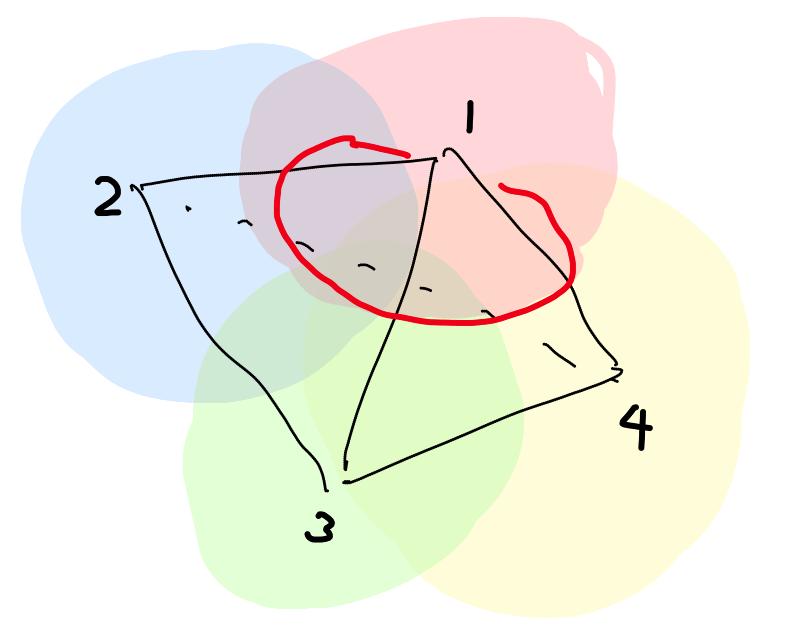
\includegraphics[width=.3\textwidth]{c1.png}
\caption{A 2-cycle $C$ on $M$ \label{fig:2cycle}}
\end{figure}

The pairing $\langle c_1(P),C\rangle$ is by definition 
the sum of $c(i,j,k)$ over four triangles there.
In this particular case, we can take the equator to cross the edges $12$, $13$ and $14$ so that $g_{23}(x)=g_{34}(x)=g_{42}(x)=1$. 
We take $g_{12}(x)$, $g_{13}(x)$ and $g_{14}(x)$ to be the patching function $g(x)$ on the equator restricted to the overlap of patches $U_{12}$, $U_{13}$ and $U_{14}$.
For ease of computation we can set $g_{13}(x)=g_{14}(x)=1$ 
and the only nontrivial thing happens in $g_{12}(x)$.
Then the only nontrivial $\theta_{ij}(x)$ is $\theta_{12}(x)$.
$\theta_{12}(x_3)$ on $x_3\in U_{123}$ is an integer independent of $x_3$, which is $c(1,2,3)$. 
Similarly, $\theta_{12}(x)$ on $x\in U_{124}$ is an integer independent of $x_4$, which is $c(1,2,4)$.
$c(1,3,4)$ and $c(2,3,4)$ are zero by definition.
Therefore the pairing is given by \begin{equation}
\langle c_1(P),C\rangle = c(1,2,3) - c(1,2,4) = \theta_{12}(x_3)-\theta_{12}(x_4),
\end{equation} which is the winding number of $g(x)$ on the equator. 

Therefore it characterizes the topological class of the bundle $P$ over the 2-cycle $C$.
Combining with our discussion of the de Rham cohomology class $[F/(2\pi)]\in H^2(M,\bR)$ associated to a connection of the $U(1)$ bundle, 
we have found the following important relation:
\begin{proposition}
  The first Chern class $c_1(P)$ of a principal $U(1)$ bundle $U(1)\to P\to M$ 
  satisfies 
  \begin{equation}
    \langle c_1(P),C\rangle = \int_C \frac{F}{2\pi},
  \end{equation}
  where $F$ is the curvature 2-form of the connection on the same bundle.
\end{proposition}

Note that the 2-form $F/(2\pi)$ is defined with real numbers but somehow integrates to an integer,
whereas $c_1(P)$ is intrincially defined with $\bZ$.
For example, there is a principal $U(1)$ bundle over $S^3/\bZ_2$
for which $F$ is zero but $c_1(P)$ is nontrivial.

\subsubsection{Second Stiefel-Whitney class of an $SO(3)$ bundle}

Let us now suppose that we are given an $SO(3)$ bundle $SO(3)\to P\to M$.
This is given by the data of the transition functions $g_{ij}(x)\in SO(3)$
between patches $U_i$ and $U_j$.
For consistency, they satisfy $g_{ij}(x)g_{jk}(x)g_{ki}(x)=1$ on a triple overlap.

Let us consider when there is a lift to an $SU(2)$ bundle $SU(2)\to \tilde P\to M$.
Let us denote by $p$ the projection map $p:SU(2)\to SO(3)$.
If there is a lift, then there will be transition functions $\tilde g_{ij}(x)\in SU(2)$ such that \begin{align}
  p(\tilde g_{ij}) &= g_{ij}, \label{eq:lift}\\
  \tilde g_{ij}(x)\tilde g_{jk}(x)\tilde g_{ki}(x) &= 1.\label{eq:consistency}
\end{align}
When will we be able to find such functions?

We assumed that each overlap $U_{ij}=U_i\cap U_j$ is contractible, 
so we can work over each patch to find $\tilde g_{ij}(x)\in SU(2)$ satisfying 
the first equation \eqref{eq:lift} above.
But the second equation \eqref{eq:consistency} is not guaranteed. 

Suppose that we chose $\tilde g_{ij}(x)$ over $U_{ij}$ so that \eqref{eq:lift} is satisfied.
We now have \begin{equation}
p(\tilde g_{ij}(x)\tilde g_{jk}(x)\tilde g_{ki}(x)) = g_{ij}(x)g_{jk}(x)g_{ki}(x)=1,
\end{equation}
therefore \begin{equation}
\tilde g_{ij}(x)\tilde g_{jk}(x)\tilde g_{ki}(x) = \pm 1, \label{eq:this-quantity}
\end{equation} in view of the short exact sequence \begin{equation}
1\to \bZ_2 \to SU(2)\to SO(3)\to 1.
\end{equation}
Let us define $w(i,j,k)$ by this quantity \eqref{eq:this-quantity}.
We can show that $w(i,j,k)$ is antisymmetric under the interchange of $i,j,k$,

We now have \begin{equation}
w(i,j,k)w(i,k,l)= p(\tilde g_{ij} \tilde g_{jk}\tilde g_{ki} ) 
p(\tilde g_{ik} \tilde g_{kl} \tilde g_{li})
=p(\tilde g_{ij} \tilde g_{jk}\tilde g_{kl} \tilde g_{li})
\end{equation} and similarly \begin{equation}
  w(l,i,j)w(l,j,k)= p(\tilde g_{li} \tilde g_{ij}\tilde g_{jl} ) 
  p(\tilde g_{lj} \tilde g_{jk} \tilde g_{kl})
  =p(\tilde g_{li}\tilde g_{ij} \tilde g_{jk}\tilde g_{kl} )  
\end{equation} and therefore \begin{equation}
  w(i,j,k)w(i,k,l) = w(l,i,j)w(l,j,k),
\end{equation}  meaning that $\delta w=0$.
Therefore $w$ is a \v Cech 2-cocycle, defining a cohomology class $[w]\in H^2(M;\bZ_2)$.


If we choose a different lift $\hat g_{ij}(x)\in SU(2)$, then we have 
$\hat g_{ij}(x)= f_{ij} g_{ij}(x)$ for some $f_{ij}\in \bZ_2$.
BY a short computation we find that 
\begin{equation}
\hat w(i,j,k) = w(i,j,k) + (\delta f)(i,j,k)
\end{equation} (where we use an additive notation) and therefore $[w]=[\hat w]$.

Note that $w=0$ and $[w]=0$ if $\tilde g_{ij}(x)\in SU(2)$ satisfies \eqref{eq:consistency}.
Convesely, if $[w]=0$, there is a choice of $f_{ij}\in \bZ_2$ such that $\hat g_{ij}(x)= f_{ij} g_{ij}(x)$ has $\hat (w,i,k)=0$ for all $i,j,k$,
meaning that $\hat g_{ij}(x) \hat g_{jk}(x)\hat g_{ki}(x)=1$.
This means that the $SO(3)$ bundle $SO(3)\to P\to M$ lifts to an $SU(2)$ bundle $SU(2)\to \tilde P\to M$.

Summarizing, we found the following theorem:
\begin{theorem}
  We can associate a cohomology class $w_2(P)\in H^2(M;\bZ_2)$ to an $SO(3)$ bundle $SO(3)\to P\to M$,
  such that $w_2(P)=0$ if and only if the bundle $P$ lifts to an $SU(2)$ bundle.
  This $w_2(P)$ is called the second Stiefel-Whitney class of $P$.
\end{theorem}

\begin{remark}
  Therefore, the second Stiefel-Whitney class $w_2(P)$ is the obstruction of the bundle to be an $SU(2)$ bundle.
\end{remark}

Let us give two simple examples of a bundle with nontrivial $w_2(P)$.
Over a 2-sphere $S^2$, take the northern and southern hemispheres $U_N$ and $U_S$ as the two patches.
An $SO(3)$ bundle is specified by a map from the equator to $SO(3)$, $g:S^1\to SO(3)$. 
They are classified by $\pi_1(SO(3))=\bZ_2$.
The pairing of $w_2(P)$ on $S^2$, $\langle w_2(P),S^2\rangle$, is given by this number in $\bZ_2$.

Simiarly, an $SU(2)$ bundle over $S^2$ is specified by $\tilde g: S^1\to SU(2)$.
The map $p:SU(2)\to SO(3)$ gives a map $\pi_1(SU(2))\to \pi_1(SO(3))$.
As $\pi_1(SU(2))=0$,
any $SU(2)$ bundle regarded as an $SO(3)$ bundle 
corresponds to the trivial class in $\pi_1(SO(3))=\bZ_2$.

\begin{example}
Consider the $SO(3)$ bundle over $S^2$ given by 
the map $g: S^1\to SO(3)$ which corresponds to a $360^\circ$ rotation within $SO(3)$, so that $[g]\in \pi_1(SO(3))=\bZ_2$ is nontrivial.
This bundle has $\langle w_2(P),S^3\rangle=1$ and cannot be lifted to an $SU(2)$ bundle.
\end{example}

Let us next consider an $SO(3)$ bundle over $T^2$.
We construct this by thinking $T^2$ as a quotient of $\bR^2$ parameterized by $(s,t)$ under the identification $(s,t)\sim (s+1,t)\sim (s,t+1)$.
We start from a trivial $\bR^3$ bundle over $\bR^2$ given by
$\bR^2\times \bR^3$, parameterized by $(s,t;x,y,z)$.
We now make two identifications:
\begin{align}
  (s,t;x,y,z) &\sim (s+1,t;-x,-y,z),\label{eq:SO3foo}\\
  (s,t;x,y,z) &\sim (s,t+1;x,-y,-z).\label{eq:SO3bar}
\end{align}
The first is associated to the $SO(3)$ transformation $\mathrm{diag}(-1,-1,1)$,
and the second to $\mathrm{diag}(1,-1,-1)$.

Let us try to lift this to an $SU(2)$ bundle. 
We start from $\bR^2\times \bC^2$, parameterized by $(s,t;v)$.
A lift of $\mathrm{diag}(-1,-1,1)\in SO(3)$ to $SU(2)$ is simply $\sigma_z$,
and a lift of $\mathrm{diag}(1,-1,-1)\in SO(3)$ to $SU(2)$ is $\sigma_x$.
So we try to perform the following identifications:
\begin{align}
  (s,t;v) &\sim (s+1,t;\sigma_z v),\\
  (s,t;v) &\sim (s,t+1;\sigma_x v).
\end{align}
But this is inconsistent, since \begin{equation}
  (s,t;v)\sim (s+1,t;\sigma_z v)\sim (s+1,t+1;\sigma_x\sigma_x v)
\end{equation} and \begin{equation}
  (s,t;v)\sim (s,t+1;\sigma_x v)\sim (s+1,t+1;\sigma_z\sigma_x v)
\end{equation} but \begin{equation}
  \sigma_x\sigma_x = - \sigma_z\sigma_x.
\end{equation}
This means that the $SO(3)$ bundle over $T^2$ defined by \eqref{eq:SO3foo} and \eqref{eq:SO3bar} cannot be lifted to an $SU(2)$ bundle,
and that $\langle w_2(P),T^2\rangle=1 \in \{0,1\}=\bZ_2$.

\subsubsection{Second Stiefel-Whitney class of an $SO(n)$ bundle}


We can replace $0\to \bZ_2\to SU(2)\to SO(3)\to 0$ by $0\to \bZ_2\to Spin(n)\to SO(n)\to 0$, and conclude 
\begin{proposition}
  We can associate a characteristic class, called
  the second Stiefel-Whitney class $w_2(P)$,
  to an $SO(n)$ bundle $SO(n)\to P\to M$.
  This characteristic class vanishes, $w_2(P)=0$, if and only if the bundle $P$ lifts to a principal $Spin(n)$ bundle.
\end{proposition}


Given a manifold $M$, we can consider its tangent bundle $TM$, which is an associated vector bundle to an $O(n)$ bundle.
If $M$ is orientable, $w_1(TM)=0$, and $TM$ is an $SO(n)$ bundle.
We can ask if it can be further lifted to $Spin(n)$.
We learned that this is controled by the second Stiefel-Whitney class $w_2(TM)$ of $M$.
Summarizing, we have the following proposition:
\begin{proposition}
The second Stiefel-Whitney class $w_2(M)$ of a manifold $M$ is zero if and only if $M$ is spin.
\end{proposition}

Although we cannot prove it yet, we have the following important theorem:
\begin{theorem}
Any orientable manifold of dimension $\leq 3$ is spin.
\end{theorem}

\begin{remark}
There is a non-spin manifold of dimension 4. An example is $\CP^2$.
\end{remark}

%\subsubsection{General degree-2 obstruction classes}

By going over the construction of $c_1(P)$ of a $U(1)$ bundle and 
of $w_2(P)$ of an $SO(n)$ bundle again,
we see that the procedure is completely parallel.
Namely, for the former, we used the sequence \begin{equation}
0\to \bZ\to \bR \to U(1)\to 0 
\end{equation} whereas in the latter, for $SO(3)$ we used \begin{equation}
0\to \bZ_2\to SU(2)\to SO(3)\to 0
\end{equation} and more generally we used \begin{equation}
0\to \bZ_2\to Spin(n)\to SO(n)\to 0.
\end{equation}

The same argument can be applied to any short exact sequence of groups \begin{equation}
0\to A\to \Gamma \to G\to 0
\end{equation} for which $A$ is a discrete Abelian group,
namely:
\begin{proposition}
  Given a principal $G$ bundle $G\to P\to M$,
  we can associate a cohomology class $v_2(P)\in H^2(M;A)$,
  such that $v_2(P)=0$ if and only if the bundle $P$ lifts to a principal $\Gamma$ bundle.
\end{proposition}

\subsection{A characteristic class in $H^3(M;A)$}

We discussed the question of lifting an $SO(3)$ bundle to an $SU(2)$ bundle above.
This was a natural question in the physics context of considering 
the action of the rotation group $SO(3)$ on a wavefunction transforming as a spinor.

In a more general quantum mechanical context, a real three-dimensional space
also arise as the space of Hermitean operators $\sigma_{x,y,z}$
of a two-level system, or a qubit.
An $\bR^3$ bundle, or equivalently an $SO(3)$ bundle over a parameter space $M$
can be thought of as a family of a qubit over $M$,
described in terms of observables or dually, in terms of density matrices. 
A $\bC^2$ bundle, or equivalently a $U(2)$ bundle over $M$, 
can also be thought of as a family of a qubit over $M$.
We can wonder if there are subtle distinctions between the two.

\subsubsection{An example}

Before discussing the general theory, let us consider an example.
Take the $\bR^3$-bundle over $T^2$ given by the identifications \eqref{eq:SO3foo} and \eqref{eq:SO3bar} above.
It cannot be lifted to $SU(2)$. Can we lift it to $U(2)$?
Yes it is; we simply take the identifications \begin{align}
  (s,t;v) &\sim (s+1,t;\sigma_z v),\\
  (s,t;v) &\sim (s,t+1;e^{\pi \I s}\sigma_x v).
\end{align}
These identifications are now consistent, since \begin{equation}
  (s,t;v)\sim (s+1,t;\sigma_z v)\sim (s+1,t+1;e^{\pi \I (s+1)}\sigma_x\sigma_z v)
\end{equation} whereas \begin{equation}
  (s,t;v)\sim (s,t+1;e^{\pi \I s}\sigma_x v)\sim (s+1,t+1;e^{\pi \I s}\sigma_z\sigma_x v).
\end{equation}

Given a $U(2)$ bundle, we can take its determinant $\det:U(2)\to U(1)$ to get a $U(1)$ bundle. 
Call it $L\to M$ 
Taking its coorindate to be $w$, we find the identificaiton \begin{align}
  (s,t;w) &\sim (s+1,t;w),\\
  (s,t;w) &\sim (s,t+1;e^{2\pi I s}w).
\end{align}
This means that the determinant $U(1)$ bundle $L$ of the $U(2)$ bundle over $T^2$
lifting our $SO(3)$ bundle has a nontrival first Chern class $c_1(L)$,
satisfying $\langle c_1(L),T^2\rangle=1$.
This can be shown more generally:
any $U(2)$ bundle over $T^2$ lifting our $SO(3)$ bundle 
has a nontrivial first Chern class which is odd: $\langle c_1(L),T^2\rangle=1$ modulo 2.

This observation can be used to construct an example
where an $\bR^3$ bundle over $M$ cannot be lifted to a $U(2)$ bundle.
To do this, simply add another coordinate $u\sim u+1$ to $T^2$,
but with a twisted identification \begin{equation}
(s,t,u) \sim (s+1,t,u),\quad
(s,t,u) \sim (s,t+1,u),\quad
(s,t,u) \sim (s,-t,u+1).
\end{equation}
This makes the total parameter space to be $S^1$ (parameterized by $s$)
times a Klein bottle (parameterized by $t,u$).
We take the $\bR^3$ bundle over this space given by the identifications \eqref{eq:SO3foo} and \eqref{eq:SO3bar} above,
without the $u$-dependence. More precisely, we take the identifications \begin{align}
  (s,t,u;x,y,z) &\sim (s+1,t,u;-x,-y,z),\\
  (s,t,u;x,y,z) &\sim (s,t+1,u;x,-y,-z),\\
  (s,t,u;x,y,z) &\sim (s,-t,u+1;x,y,z).
\end{align}

To see that this cannot be lifted to a $U(2)$ bundle, we can use the following argument.
Suppose there is a $U(2)$ bundle lifting it.
At constant fixed $u=u_0$, the determinant $U(1)$ bundle $L\to T^2$
has a nontrivial value $\langle c_1(L),T^2\rangle = 1 $ mod 2.
We can continuously change $u_0$.
As we go around the $u$-circle, the value $ \langle c_1(L),T^2\rangle$
cannot change, since it is an integer.
However, the twisted identification $(t,u)\sim (-t,u+1)$
requires that the orientation of $T^2$ is reversed as we go around the $u$-circle,
so $\langle c_1(L),T^2\rangle$ must change its sign.
This is a contradiction, and therefore the $\bR^3$ bundle over $T^2\times S^1$ cannot be lifted to a $U(2)$ bundle.

As will be explained now, this impossiblity to lift is 
due to the existence of the obstruction class in $H^3(M;\bZ)$.
On $T^2$, $H^3(T^2;\bZ)=0$, and the obstruction was simply absent,
which explains why the $SO(3)$ bundle over $T^2$ could be lifted to a $U(2)$ bundle.
On a three-dimensional space, however, the obstruction can in general be nontrivial,
leading to the impossibility of lifting the $SO(3)$ bundle to a $U(2)$ bundle.

\if0
\begin{remark}
It appears that there are some circles of theoretical physicisits studying 
quantum mechanics and/or quantum information,
where people think that density matrices have 
the same descriptive power as wavefunctions.
The example above shows that this is not quite true,
when we consider a continuous family of such systems over a parameter space.
\end{remark}
\fi

\subsubsection{General theory}

So, let us ask when an $SO(3)$ bundle $SO(3)\to P\to M$ can be lifted to a $U(2)$ bundle $U(2)\to \tilde P\to M$.
As always, take a fine enough cover $U_i$, so that all nonempty intersections $U_{i_1}\cap U_{i_2}\cap \cdots \cap U_{i_k}$ are contractible.
The data of the $SO(3)$ bundle is given by the transition functions $g_{ij}(x)\in SO(3)$, satisfying \begin{equation}
  g_{ij}(x)g_{jk}(x)g_{ki}(x)=1.
\end{equation}

We already discussed the lifting to $SU(2)$. 
To reuse some of the discussions,
it is useful to think of \begin{equation}
U(2) = \frac{U(1)\times SU(2)}{\bZ_2}, \label{eq:U2}
\end{equation} where $\bZ_2 \subset U(1)\times SU(2)$ is generated by $(-1,-1)$.
Indeed, any $2\times 2$ unitary matrix $U$ can be written as \begin{equation}
U= e^{2\pi\I \theta} \tilde U
\end{equation} where $\det\tilde U=1$, but this splitting is not unique;
we have an ambiguity of $(e^{2\pi\I \theta},\tilde U) \sim (-e^{2\pi\I \theta},-\tilde U)$.

A $U(2)$ bundle is specified by the transition functions $\tilde g_{ij}(x)\in U(2)$, satisfying \begin{equation}
  \tilde g_{ij}(x)\tilde g_{jk}(x)\tilde g_{ki}(x)=1.
\end{equation}
Using \eqref{eq:U2}, it can also be given by pairs \begin{equation}
(e^{2\pi\I\theta_{ij}(x)},h_{ij}(x))\in U(1)\times SU(2)
\end{equation} satisfying \begin{align}
  e^{2\pi\I\theta_{ij}(x)}e^{2\pi\I\theta_{jk}(x)}e^{2\pi\I\theta_{ki}(x)}&=(-1)^{w_{ijk}},\label{eq:rel-theta}\\
  h_{ij}(x)h_{jk}(x)h_{ki}(x)&=(-1)^{w_{ijk}},\label{eq:rel-h}
\end{align}
where $w_{ijk}\in \{0,1\}$ defined on each $U_{ijk}$.

For this $U(2)$ bundle to lift a given $SO(3)$ bundle, we simply need to have \begin{equation}
p(h_{ij})=g_{ij}.
\end{equation}
This is the condition we repeatedly used in the previous section,
where we learned that the condition \eqref{eq:rel-h}
implies that  $w_{ijk}$ is a \v Cech 2-cocycle,
defining a cohomology class $[w]\in H^2(M;\bZ_2)$.
The condition \eqref{eq:rel-theta} imposes an additional constraint.

To see this, consider \begin{equation}
  n_{ijk}(x):=2(\theta_{ij}(x)+\theta_{jk}(x)+\theta_{ki}(x)).\label{eq:n}
\end{equation}
From \eqref{eq:rel-theta} we know it is actually a constant $n_{ijk}$ on each $U_{ijk}$,
which satisfies \begin{equation}
  n_{ijk} = w_{ijk} \mod 2.\label{eq:nw}
\end{equation}


$n_{ijk}$ is actually a \v Cech 2-cocycle, defining a cohomology class $[n]\in H^2(M;\bZ)$.
To see this, we note that the determinant map $\det:U(2)\to U(1)$ 
sends $(e^{2\pi\I\theta},h)\mapsto e^{2\pi\I\cdot 2\theta}$.
Therefore the patching functions $e^{2\pi\I\cdot 2\theta_{ij}(x)}$ define a principal $U(1)$ bundle $U(1)\to L\to M$,
and the relation \eqref{eq:n} says that $n_{ijk}$ is the \v Cech 2-cocycle 
giving its first Chern class $c_1$.
This means that the cohomology class $w_2(P)\in H^2(M;\bZ_2)$ of the $SO(3)$ bundle 
is the mod-2 reduction of the cohomology class $c_1(L)\in H^2(M;\bZ)$ of the $U(1)$ bundle $L$.

Conversely, suppose that, for a given $SO(3)$ bundle $SO(3)\to P\to M$,
there is a $U(1)$ bundle $U(1)\to L\to M$ 
such that $w_2(P)$ is the mod-2 reduction of $c_1(L)$.
Let $g_{ij}(x)\in SO(3)$ be the transition functions of $P$,
and $h_{ij}(x)\in SU(2)$ be their lifts to $SU(2)$.
Let $e^{2\pi \I \cdot 2\theta_{ij}(x)}$ be the patching functions of $L$,
and define $w$ and $n$ as above.
The condition that the cohomology classes (not the cocycles themselves)
satisfy $w_2(P)=c_1(L)$
 means that we have \begin{equation}
  n_{ijk} +(\delta m)_{ijk}= w_{ijk} +(\delta v)_{ijk} \mod 2.
\end{equation}
This means that we can re-take $\theta_{ij}(x)\mapsto \theta_{ij}(x)+ m_{ij}/2 $ and $h_{ij}(x)\mapsto h_{ij}(x) (-1)^{v_{ij}}$
so that the relation \eqref{eq:nw} is satisfied on the nose,
which gives a lift of the $SO(3)$ bundle to a $U(2)$ bundle.



Summarizing our discussion so far, we have the following proposition:
\begin{proposition}
  An $SO(3)$ bundle $SO(3)\to P\to M$
  lifts to a $U(2)$ bundle $U(2)\to \tilde P\to M$ if and only if
   $w_2(P)\in H^2(M;\bZ_2)$ is 
  the mod 2 reduction of a class $c\in H^2(M;\bZ)$ .
\end{proposition}
where we used the fact that any class $c\in H^2(M;\bZ)$ is
the first Chern class of some principal $U(1)$ bundle $L$ over $M$ 
(which we have not proved but will prove in the next section).

We now need to study when a class $w\in H^2(M;\bZ_2)$ is the mod-2 reduction of a class $c\in H^2(M;\bZ)$.
The class $w$ is represented by a \v Cech 2-cocycle $w_{ijk}\in \bZ_2$.
When it is a mod-2 reduction of a class $c\in H^2(M;\bZ)$,
we can pick a lift $c_{ijk}$ which is a \v Cech 2-cocycle in $\bZ$.

But it is not always the case that there is such a cocycle lift.
Pick any lift $c_{ijk}\in \bZ$ of $w_{ijk}$.
This is a cochain, but is not guaranteed to be a cocycle.
Let us study its failure to be a cocycle.
We have \begin{equation}
(\delta c)_{ijkl} = c_{jkl}-c_{ikl}+c_{ijl}-c_{ijk} 
\end{equation} which is always even because \begin{equation}
  = w_{ijk}+w_{jkl}+w_{kli}+w_{lij} = (\delta w)_{ijkl}=0\mod 2.
\end{equation}
Let us define, then, \begin{equation}
  d_{ijkl} = \frac12(c_{jkl}-c_{ikl}+c_{ijl}-c_{ijk})\in \bZ.
\end{equation}
This is a \v Cech 3-cocycle, because \begin{equation}
(\delta d)_{ijklm} = \frac12 (\delta\delta c)_{ijklm} =0.
\end{equation}
We have thus defined a class $[d]\in H^3(M;\bZ)$.
By construction, this class vanishes if there is a cocycle lift $c_{ijk}$ of $w_{ijk}$.

Conversely, if this class vanishes, we have a cochain $d=\delta e$.
We then define $c_{ijk}+2e_{ijk}$ to be the new lift of $w_{ijk}$;
by construction it is a cocycle.

So we learned that the class $w\in H^2(M;\bZ_2)$ is the mod-2 reduction of a class $c\in H^2(M;\bZ)$ 
if and only if the class $[d]\in H^3(M;\bZ)$ constructed above vanishes.
The consturction might have looked rather ad hoc, 
so let us slightly generalize the construction.

Let us take a short exact sequence of Abelian groups \begin{equation}
  0\to A\to B\to C\to 0.
\end{equation}
The case discussed above corresponds to the case \begin{equation}
  0\to \bZ\xrightarrow{\times2} \bZ\xrightarrow{\mod2} \bZ_2\to 0.
\end{equation}
We study when a class $w\in H^2(M;C)$ comes from a class $c\in H^2(M;B)$.
For this purpose, take a cocycle representative $w_{ijk}\in C$ of $w$,
and take an arbitrary lift $c_{ijk}\in B$.
By construction, $(\delta c)_{ijkl}$ is in the kernel of $B\to C$,
i.e.~in the image of $A\to B$.
Therefore we can write \begin{equation}
  (\delta c)_{ijkl} = d_{ijkl}
\end{equation} for some $d_{ijkl}\in A$.
This defines a \v Cech 3-cocycle $[d]\in H^3(M;A)$.
The class $w\in H^2(M;C)$ comes from a class $c\in H^2(M;B)$ if and only if $[d]\in H^3(M;A)$ vanishes.
Let us summarize:

\begin{definition}
  The homomorphism $\beta:H^2(M;B)\to H^3(M;A)$
  constructed above, associated to the short exact sequence $0\to A\to B\to C\to 0$,
  is called the Bockstein homomorphism.
\end{definition}

\begin{proposition}
  A class $w\in H^2(M;C)$ comes from a class $c\in H^2(M;B)$
  if and only if its Bockstein $\beta(w)\in H^2(M;A)$ vanishes.
\end{proposition}

Coming back to the question of the lift of an $SO(3)$ bundle to a $U(2)$ bundle,
we now have the following proposition:
\begin{proposition}
  An $SO(3)$ bundle $SO(3)\to P\to M$
  lifts to a $U(2)$ bundle $U(2)\to \tilde P\to M$ if and only if
  the Bockstein $\beta(w_2(P))\in H^3(M;\bZ)$ vanishes.
\end{proposition}

\begin{remark}
Therefore, the degree-3 class $\beta(w_2(P))$ 
is the obstruction of the $SO(3)$ bundle to be lifted to a $U(2)$ bundle.
$\beta(w_2(P))$ is also known as the integral third Stiefel-Whitney class of the $SO(3)$ bundle, 
and is denoted by $W_3(P)$.
The more ordinary third Stiefel-Whitney class $w_3(P)\in H^3(M;\bZ_2)$ is the mod-2 reduction of $W_3(P)$.
\end{remark}

\begin{question}
Here we only discussed the case of lifting an $SO(3)$ bundle to a $U(2)$ bundle,
which corresponds to the question of density matrices of 2-level systems (i.e.~qubits).
What happens when we consider $n$-level systems instead,
where the symmetry is $U(n)$ acting on the Hilbert space $\bC^n$,
while the symmetry acting on the density matrices is \begin{equation}
PU(n):=\frac{U(n)}{U(1)} = \frac{U(1)\times SU(n)}{\bZ_n},
\end{equation}where $\bZ_n$ is embedded in $U(1)\times SU(n)$ as $(e^{2\pi I/n},e^{-2\pi I/n})$?
\end{question}

\subsection{Classifying spaces}
\subsubsection{For principal $G$-bundles}

We now introduce the concept of the classifying space of principal $G$-bundles.

\begin{definition}
The base $B$ of a principal $G$ fiber bundle $G\to E\to B$ such that 
$\pi_k(E)=0$ for any $k$
is called a classifying space and is denoted by $BG$.
We denote the entire fiber bundle by $G\to EG\to BG$.
\end{definition}

\begin{remark}
It is not immediate that such a classifying bundle $EG\to BG$ exists,
or it is unique if it exists. 
It turns out that such an $EG\to BG$ always exists, and is homotopically unique.
\end{remark}

As an example, recall the $U(1)$ fiber bundle $U(1)\to S^{2n+1}\to \CP^n$.
This satisfies $\pi_k(S^{2n+1})=0$ up to $k<2n+1$.
Therefore, by suitably taking the limit $n\to \infty$, we see
\begin{example}
$BU(1)=\CP^n$.
\end{example}

The importance of the concept of the classifying space comes from the following:

\begin{theorem}
\label{thm:classifying}
Any principal $G$ bundle $E\to X$ over any space $X$ is obtained by pulling back $EG\to BG$ by a map $f: X\to BG$.
Furthermore, there is a one-to-one correspondence between
principal $G$ bundles over $X$ up to equivalence
and maps $f:X\to BG$ up to homotopy.
\end{theorem}

\begin{proof}(of Theorem \ref{thm:classifying})
We already quoted a theorem (Theorem~\ref{thm:bundle-equiv}) saying that 
two homotopic maps $f,f': X\to Y$ gives two equivalent bundles under the pull-back.
So we only have to show that such a map $f:X\to BG$ can be constructed, 
from a principal $G$-bundle $G\to E\to X$.
We assume $X$ is given  the structure of a CW complex.
We construct the map inductively.
On the 0-th skeleton $X_0$, it is clear that we can construct a map $f_0: X_0\to BG$ such that the pull back is the $G$-bundle over $X_0$.
We now show that if we have the map up to $f:X_k\to BG$,
we can extend it to $f: X_{k+1}\to BG$.
For this, we only have to deal with each cell.
Therefore, what needs to be done is the following:
given a principal $G$-bundle $E\to B^{k+1}$,
together with a map $f: S^k \to BG$ such that the pull-back $f^*(EG)\to S^k$ agrees with $E$ restricted to its boundary,
construct a map $f:B^k\to BG$ such that the statement holds.

To do this, we note that any bundle $G\to E\to B^{k+1}$ is topologically trivial, 
and therefore its restriction on the boundary $S^k$ is also topologically trivial.
This means that it has a section $S^k \to E$.
Using the equivalence of $E\to S^k$ and $f^*(EG)\to S^k$,
we can consider this section as a map $S^k \to EG$.
As $\pi_{k}(EG)=0$ from assumption, we can extend this map to $B^{k+1}\to EG$.
Composing with the projection $EG\to BG$, we have extended the map to $B^{k+1}\to BG$.
It is routine to check that the map thus obtained satisfies the required properties.
\end{proof}

\begin{remark}
That $BU(1)=\CP^\infty$ was infinite dimensional might have been worrying to you.
But the proof above shows that, to classify principal $G$-bundles over $X$ of dimension at most $n$,
we only have to demand $\pi_{k}(BG)=0$ up to $k<n$.
Therefore, $\CP^n$ with finite but sufficiently large $n$ suffices for most of the purpose of theoretical physicists.
Taking $n$ infinity does however simplify statements of theorems etc., 
which is why it is conventional to use infinite dimensional classifying spaces.
\end{remark}

The existence of classifying spaces is a nontrivial theorem:
\begin{theorem}
The classifying bundle $G\to EG\to BG$ exists for any group $G$.
\end{theorem}
which we do not have the time to go into.
But the uniqueness up to homotopy is a simple corollary of the theorem above:
\begin{proposition}
Two classifying bundles $EG\to BG$ and $E'G\to B'G$ are homotopically the same.
\end{proposition}
\begin{proof}
By the theorem above, we have maps $f:BG\to B'G$ and $g:B'G\to BG$ 
such that the bundles pull back to each other. 
In particular, $g\circ f: BG\to BG$ pulls back the bundle $EG\to BG$ to itself.
Therefore, $g\circ f$ is homotopic to the identify.
\end{proof}


\subsubsection{For cohomology groups}

There are also classifying spaces for cohomology groups.
For this, we need a few preparations.
\begin{definition}
For an Abelian group $A$,
any space $X$ such that $\pi_k(X)=A$ and $\pi_\ell(X)=0$ for $\ell\neq k$ is called a $K(A,k)$ space,
and is called the Eilenberg-Mac Lane space.
\end{definition}


We also need:
\begin{theorem}
For any $A$ and $k$,
$K(A,k)$ spaces exist, and are unique up to homotopy.
\end{theorem}

As an example, consider $U(1)\to S^{2n+1}\to \CP^n$ again.
From the long exact sequence in homotopy, we see $\pi_k(\CP^n)$ is nonzero only at $\pi_2=\bZ$ and $\pi_{2n+1}=\bZ$.
Suitably taking the limit $n\to \infty$,
we see that 
\begin{example}
$K(\bZ,2)=\CP^\infty$.
\end{example}

The importance of the Eilenberg-Mac Lane spaces $K(A,k)$ lies in the following.
\begin{theorem}
\label{thm:coh-cl}
For any space $X$, 
there is a one-to-one correspondence between cohomology classes $a \in H^k(X;A)$ 
and homotopy classes of maps $f: X\to K(A,k)$.
\end{theorem}
\begin{proof}
Here we only give the construction of $f$, given a cohomology class $a$.
We assume that $X$ is given the structure of a simplicial complex,
and work inductively.
We pick an explicit cocycle $a(\sigma)$ representing $a$.
As $\pi_{\ell}(X)=0$ when $\ell<k$,
we can pick a map $f:X_{k-1}\to K(A,k)$, which is homotopic to the identity.
For each $k$-simplex $\sigma$, regard it as $B^k$.
Its boundary is already mapped to the basepoint.
So we need to specify a map $S^k \to K(A,k)$.
Here we choose a map representing the element $a(\sigma)\in A=\pi_k(K(A,k))$. 
We now have a map $f:X_k \to K(A,k)$.
To extend this to $f:X_{k+1}\to K(A,k)$,
we need to extend, for each $(k+1)$-simplex $\sigma\simeq B^{k+1}$,
the already given map $S^k \to K(A,k)$
to $B^{k+1}\to K(A,k)$.
This is possible exactly because $a(\sigma)$ is a cocycle.
\end{proof}


We have seen that $\CP^\infty$ is both $BU(1)$ and $K(\bZ,2)$.
Therefore:
\begin{theorem}
\label{thm:u1-cl}
For any $X$, there is a one-to-one correspondence between principal $U(1)$ bundles over $X$
and the cohomology classes in $H^2(X;\bZ)$.
\end{theorem}
Comparing the proofs above by going into details, 
you find that the cohomology class obtained in this manner is 
$c_1$ of the $U(1)$ bundle you started with.

This can be argued in a more formal way.
For this, we go back to the general situation.
\begin{proposition}
$H^k(K(A,k);A)=\Hom(A,A)$.
\end{proposition}
\begin{proof}
This follows from Hurewicz and the universal coefficient theorem.
\end{proof}

\begin{definition}
$\iota \in H^k(K(A,k);A)$ is the identity map in $\Hom(A,A)\simeq H^k(K(A,k);A)$.
\end{definition}

We can refine Theorem \ref{thm:coh-cl} above as follows:
\begin{theorem}
The correspondence of $f: X\to K(A,k)$  and $f(\iota)\in H^k(X;A)$ is a bijection.
\end{theorem}

Now, on $BU(1)=\CP^\infty$, $H^2(\CP^\infty;\bZ)=\Hom(\bZ,\bZ)=\bZ$,
and $c_1$ of the bundle $U(1)\to S^{2\infty+1}\to \CP^\infty$ is the generator $\iota$.
Now, $c_1$ of the pullback is the pullback of $c_1$, we have succeeded in refining Theorem~\ref{thm:u1-cl} into
\begin{theorem}
For any $X$,
the correspondence between  a principal $U(1)$ bundle $U(1)\to P\to X$
and its 1st Chern class $c_1(P)\in H^2(X;\bZ)$ 
establishes a bijection between equivalence classes of principal $U(1)$ bundles over $X$
and cohomology classes in $H^2(X;\bZ)$.
\end{theorem}

\begin{corollary}
Any cohomology class  in $H^2(X;\bZ)$ is the first Chern class of a principal $U(1)$ bundle.
\end{corollary}

\subsubsection{Classifying spaces and characteristic classes}

Classifying spaces gives us a uniform way to understand characteristic classes,
which have so far been constructed in a case-by-case basis.
Suppose we are given a principal $G$ bundle $G\to P\to X$.
Correspondingly, we have a map $f_P:X\to BG$.
Now, take a cohomology class $a\in H^k(BG;A)$.
We can pull it back to $X$ to obtain $f_P^*(a)\in H^k(X;A)$.
In this manner, we have constructed a cohomology class in $H^k(X;A)$
from a given principal $G$ bundle.

For example, take $G=U(1)$.
Then $H^2(BU(1);\bZ)=H^2(\CP^\infty;bZ)=\bZ$.
Denote its generator by $c_1$.
Then, for any principal $U(1)$ bundle $U(1)\to P\to X$,
we have a map $f_P:X\to BU(1)$.
we have a cohomology class $f_P^*(c)\in H^2(X;\bZ)$.
We can identify this with the first Chern class $c_1(P)$ of the bundle $P$,
i.e.~\begin{equation}
f_P^*(c_1)=c_1(P).
\end{equation}

Similarly, for $G=SO(3)$, we have $H^2(BSO(3);\bZ_2)=\bZ_2$,
whose generator we denote by $w_2$.
Then, for any principal $SO(3)$ bundle $SO(3)\to P\to X$,
we have a map $f_P:X\to BSO(3)$.
And we have a cohomology class $f_P^*(w_2)\in H^2(X;\bZ_2)$
obtained by pulling back $w_2$.
This is the second Stiefel-Whitney class $w_2(P)$ of the bundle $P$,
i.e.~\begin{equation}
f_P^*(w_2)=w_2(P).
\end{equation}
Analogously, there is a class $W_3\in H^3(BSO(3);\bZ)$,
and \begin{equation}
f_P^*(W_3)=W_3(P).
\end{equation}

From this point of view, to determine all possible characteristic classes
for principal $G$ bundles,
one simply needs to study $H^*(BG;A)$ for various choices of $A$.
Therefore, the classification of characteristic classes
is reduced to the study of cohomology groups of classifying spaces.

\section{Chern-Simons terms}

\subsection{Quantization of the electric charges}
We saw above that the mathematical property of $U(1)$ bundles naturally leads to the Dirac quantization of the magnetic charges.
How do we understand the quantization of the electric charges? 
The way to understand it depends on whether you take the particle point of view or the wave point of view.

\subsubsection{From the wave point of view}
In the wave point of view, given a $U(1)$ bundle $P\to M$ on a spacetime $M$,
an electrically charged field is a section of an associated complex line bundle $L\to M$.
More concretely, if  the $U(1)$ bundle between two patches $U$ and $U'$ is given by \begin{equation}
U\times U(1) \supset (U\cap U')\times U(1) \ni (x,z) 
\mapsto (x,gz) \in (U\cap U')\times U(1)\subset U'\times U(1),
\end{equation} with $g:U\cap U' \to U(1)=\{g\in \bC \mid |g|=1\}$,
the allowed complex line bundles are patched by the rule \begin{equation}
U\times \bC \supset (U\cap U')\times \bC \ni (x,v) 
\mapsto (x,g^n v) \in (U\cap U')\times \bC\subset U'\times \bC.
\end{equation}
Here, $g^n$ needs to be a well-defined function, and therefore $n$ needs to be an integer. 

Let $(x,\psi(x))$ be a section of this line bundle. Then the covariant derivative we discussed in Sec.~\ref{subsec:U1connection-as-Maxwell} becomes \begin{equation}
D\psi := \sum_a\left(\frac{\partial}{\partial x^a} - i n A_a\right)\psi dx^a.
\end{equation}
The coefficient $n$ here means that the coupling between the Maxwell field $A$ and the charged field $\psi$ is proportional to $n$, 
i.e.~the electric charge is proportional to $n$. 
This is one way to understand the electric charge quantization.

\subsubsection{From the particle point of view, part I}
Let us instead use the particle point of view.
The classical action of a charged non-relativistic particle of mass $m$ and charge $q$ is \begin{equation}
S = \int \left(\frac m2 |v|^2 + q^\text{SI} (A^\text{SI}_t + \sum_a A^\text{SI}_a v^a) \right)dt 
\end{equation} where $v^a= dx^a/dt$.
Equivalently, we have \begin{equation}
S = \int \frac m2 |v|^2 dt + q^\text{SI} \int  A^\text{SI},
\end{equation} where $A^\text{SI}$ is now regarded as a 1-form and $\int A^\text{SI}$ is its integral.
This is not perfectly OK, because the vector potential $A^\text{SI}$ is not really a 1-form.
But this does not cause any problem in classical mechanics.
Indeed, given the gauge transformation \begin{equation}
A^\text{SI} \mapsto (A^\text{SI})':=A^\text{SI} + d\chi,
\end{equation} the change in the  integral is  \begin{equation}
\int_p^q (A^\text{SI})'-\int_p^q A^\text{SI} =  \chi(q)-\chi(p),
\end{equation} which depends only on the boundary values.
This does not affect the computation of the variational derivative of $S$.


In quantum mechanics this causes a problem however. 
Let us use a path integral formalism. Then we need to consider \begin{equation}
Z=\int \mathcal D x^a \exp\left( \frac{i}{\hbar}(\int_C \frac m2 |v|^2 dt  +  q^\text{here} \int_C A^\text{geometric}) \right) 
\end{equation}
where we postulate \begin{equation}
A^\text{geometric} = k A^\text{SI}
\end{equation}
with some proportionality factor $k$, so \begin{equation}
q^\text{here} = q^\text{SI}/k.
\end{equation}
$A^\text{geometric} $ gets the gauge transformation \begin{equation}
A^\text{geometric} \mapsto  (A^\text{geometric}) ' := A^\text{geometric} +  i g^{-1} d g
\end{equation}  for $g\in U(1)$.
This means that \begin{equation}
\int_C (A^\text{geometric})'
=
\int_C A^\text{geometric}
+  2\pi w
\end{equation}
where $w\in \bZ$ is the winding number of $g:C\to U(1)$.
This means that the value of the exponential gets shifted multiplicatively by \begin{equation}
\exp(\frac{2\pi i}{\hbar} q^\text{here} w ),
\end{equation} where $w$ is an arbitrary integer.
This requires us to take $q^\text{here}=\hbar n$ for some integer $n$,
i.e.~$q^\text{SI}= k \hbar n $ for some integer $n$.
This makes it reasonable to choose the proportionality factor $k$ above to be $k=e/\hbar$.

\subsubsection{From the particle point of view, part 2}

Let us derive the fact that $q^\text{here}$ needs to be an integer in a slightly different way,
suitable for a generalization later. 
When $A^\text{geometric}$ is a 1-form, and $C$ is a boundary $C=\partial D$ of a disk,
we have the theorem of Stokes, \begin{equation}
\int _C A^\text{geometric} = \int_D F^\text{geometric},
\label{eq:Stokes}
\end{equation}
assuming that the Maxwell field is also defined on $D$.
Although $A^\text{geometric}$ is not really a 1-form,
$F^\text{geometric}$ is a genuine 1-form.
So, we can try to \emph{define} the left hand side of \eqref{eq:Stokes} by the right hand side: \begin{equation}
\int _C A^\text{geometric} := \int_D F^\text{geometric}
\end{equation}
in a more general setting where $A^\text{geometric}$ is not quite a 1-form.

The right hand side is always well-defined, but we introduced a different issue.
Namely, it depends on the gauge configuration not just on $C$ but on the entirety of $D$.
To study the dependence, suppose that we extend the gauge configuration on $C$
to $D$ and $D'$ in two different ways. 
We need to study the difference of the right hand sides of \eqref{eq:Stokes} for $D$ and $D'$:
\begin{equation}
\int_{D'} F^\text{geometric} - \int_{D} F^\text{geometric} = \int_{D'\cup \overline{D}}  F^\text{geometric},
\end{equation}
see Fig.~\ref{fig:paste}.

\begin{figure}
\[
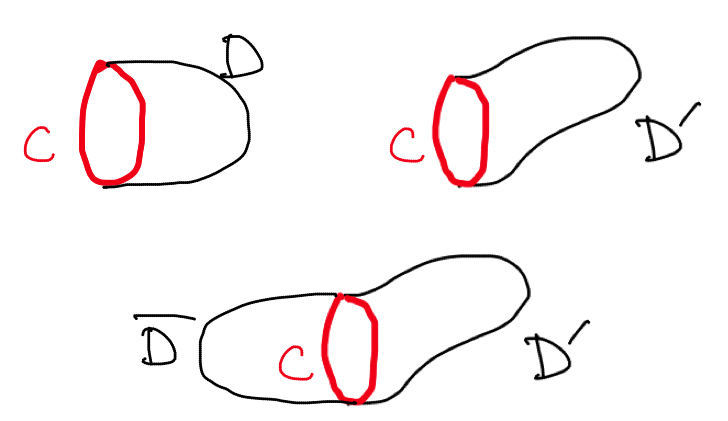
\includegraphics[width=.5\textwidth]{paste.png}
\]
\caption{The contour $C$ and the auxiliary bounding surfaces $D$ and $D'$.
\label{fig:paste}}
\end{figure}

We know that the integral of $F^\text{geometric}$ over a closed surface is quantized to be $2\pi w$ for some integer $w$.
This means that $\int_D F^\text{geometric}$ modulo $2\pi w$
is independent of the choice of the extension of the gauge configuration on $D$,
and therefore \begin{equation}
\exp(i n \int_C A^\text{geometric}) := \exp(i n \int_D F^\text{geometric})
\end{equation}
is well-defined for any integer $n$.
In particular, we have derived that $q^\text{here}=\hbar n$ for some integer $n$.

\subsection{Quantization of the Hall conductance}

\subsubsection{Physics background}
In a two-dimensional material, 
the relation between the applied voltage and the electric current is generally given by \begin{equation}
  \begin{pmatrix}
  I_x\\I_y
  \end{pmatrix}= \begin{pmatrix}
  \sigma_{xx} & \sigma_{xy}\\
  \sigma_{yx} & \sigma_{yy}
  \end{pmatrix} \begin{pmatrix}
  V_x\\V_y
  \end{pmatrix},
\end{equation} where $\sigma_{ij}$ are the components of the conductivity tensor.
In a certain experimental situation where $\sigma_{xx}=\sigma_{yy}=0$,
the Hall conductance $\sigma_{xy}$ is quantized to an integer multiple of $e^2/h$,
where $e$ is the elementary charge and $h$ is the Planck constant:
\begin{equation}
\sigma_{xy} = \nu \frac{e^2}{h}.
\label{eq:hallquant}
\end{equation}
This is known as the integer quantum Hall effect.
See Fig.~\ref{fig:experiments} for one classic and one more recent experimental results.

\begin{figure}
\[
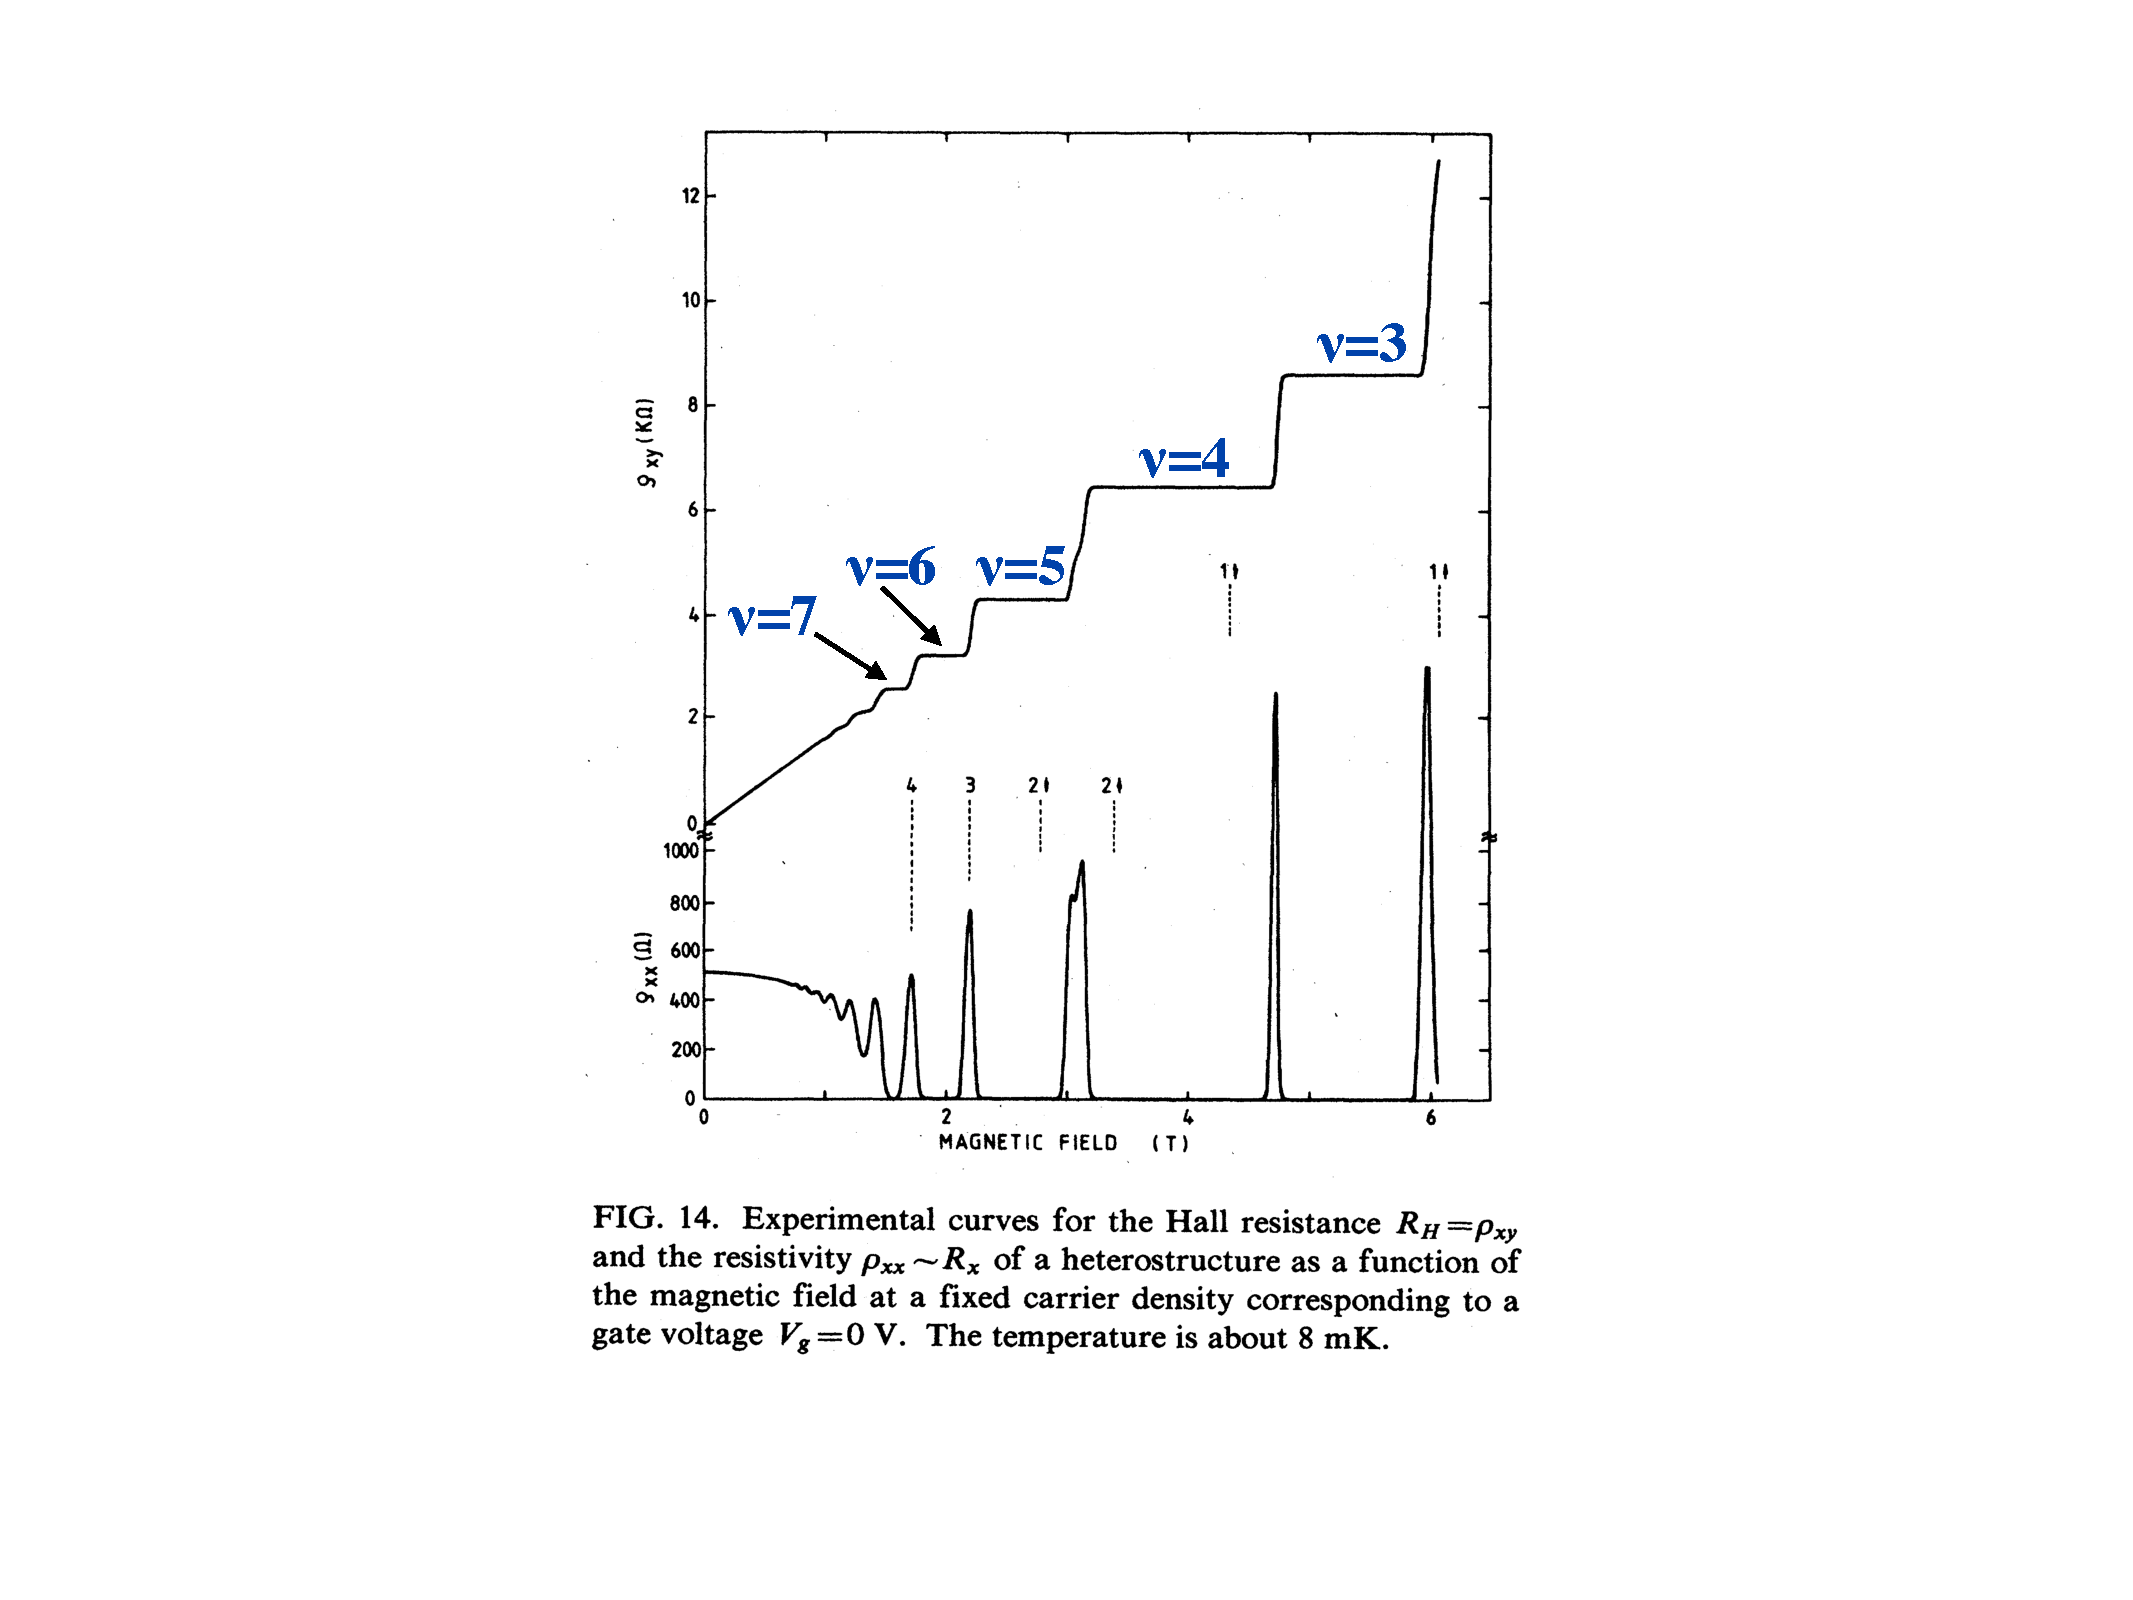
\includegraphics[width=.5\textwidth]{vK.pdf}
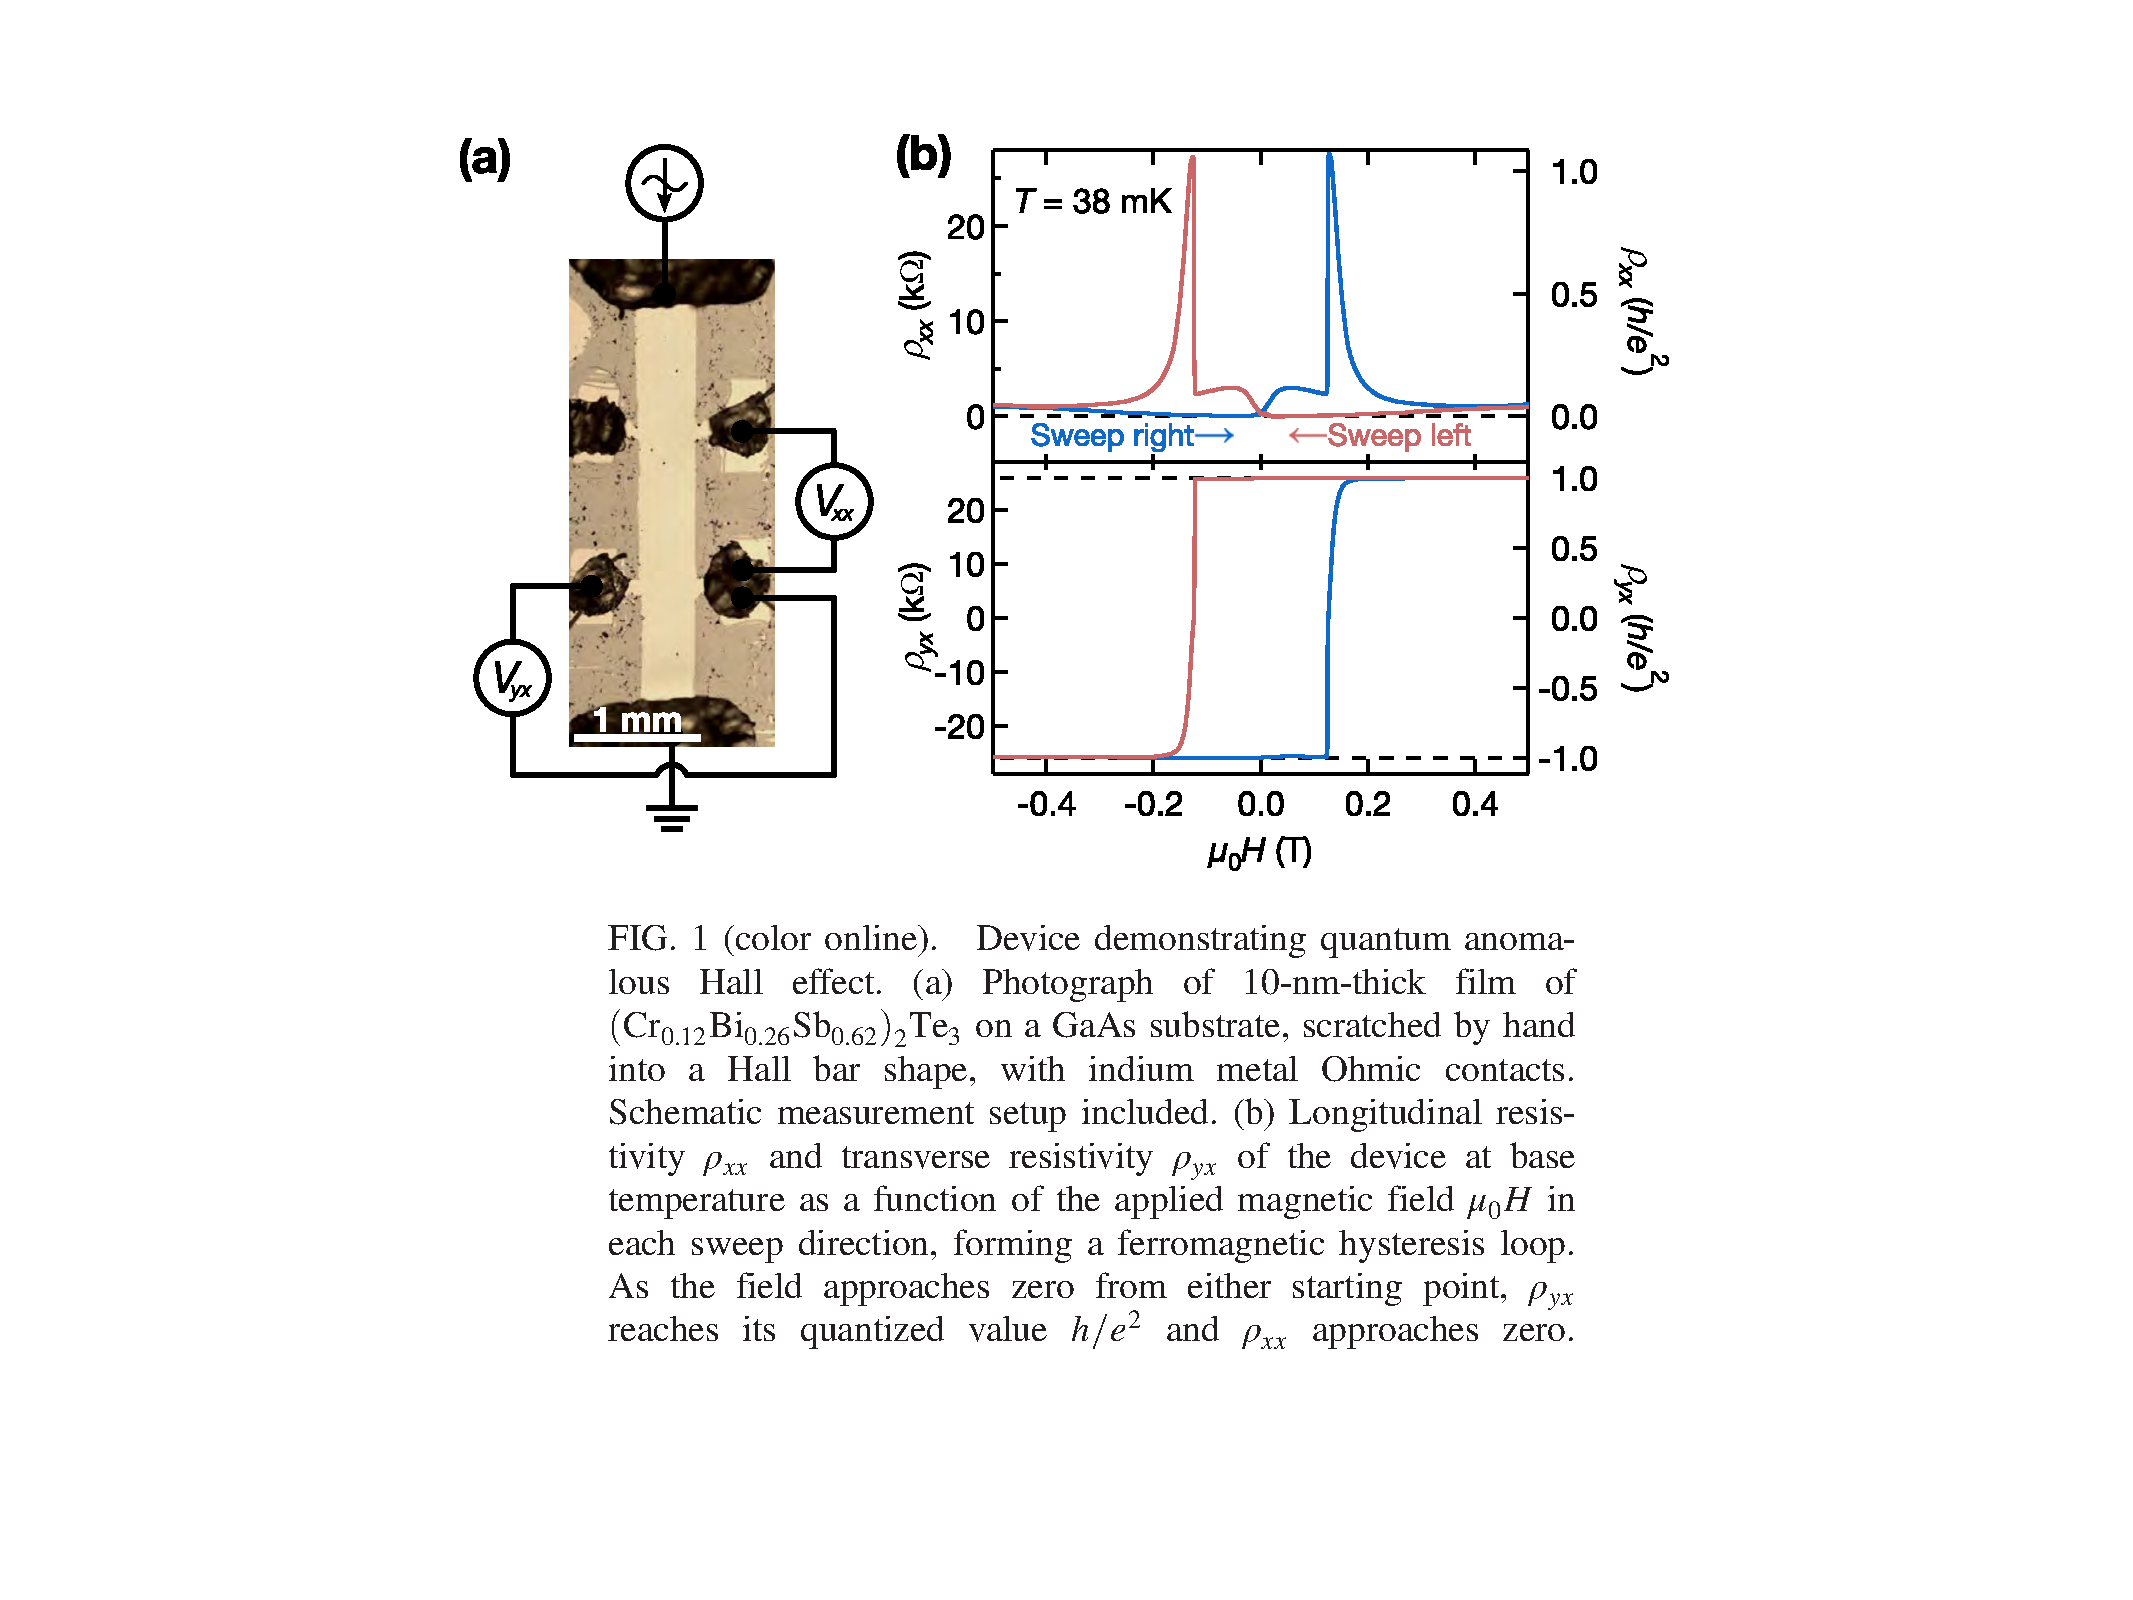
\includegraphics[width=.5\textwidth]{Bestwick.pdf}
\]
\caption{Left: from von Klitzing's classic review \cite{vK}.
Right: from a modern experiment in 2015 \cite{Bestwick}.
\label{fig:experiments}}
\end{figure}

There are various theoretical ways to understand this quantization phenomenon.
Here we would like to discuss one which is not usually discussed in the textbooks.
I am not saying that this is better than the others.
It is just that other methods are covered in many other standard textbooks,
and that this method fits very well with the content of this lecture series.

The general situation where we have the \emph{integer} quantum Hall effect is
when the system is gapped and has a unique ground state
even on a nontrivial spatial manifold such as a torus $T^2$.
In contrast, when the system is gapped but has multiple ground states
on a nontrivial spatial manifold,
the Hall conductance is quantized not to an integer but to a rational number.
This is the \emph{fractional} quantum Hall effect.
Finally if the system is not gapped the Hall conductance is not quantized.
See Table~\ref{tab:Hall} for a summary.

\begin{table}
  \centering
\begin{tabular}{c|c||c}
Gapped?  & \# of ground states & Quantization of $\sigma_{xy}$\\
\hline
Yes& unique  & Integer\\
Yes& multiple  & Rational\\
No & N/A & Not quantized
\end{tabular}
\caption{Quantization of the Hall conductance in various situations.
\label{tab:Hall}}
\end{table}

\subsubsection{Mathematical analysis}

Suppose the system is gapped and has a unique ground state.
Imagine putting the system on a nontrivial three-dimensional manifold $M_3$,
with an external Maxwell field $P\to M_3$ 
to probe the electrical property of the system.
It does not matter if this is experimentally realizable or not;
the point is the mere possibility of putting the system on such nontrivial manifolds.
The partition function $Z$ of the system 
depends on $M_3$ and the external Maxwell field $P\to M_3$.
It is dominated by the contribution from the single ground state,
and therefore is simply a phase: \begin{equation}
Z(M_3,P) = \exp( (i/\hbar) S(M_3,P))\label{eq:Zphase}
\end{equation}
where $S(M_3,P)$ should be a well-defined real number modulo integer.


When the system is gapped but with multiple ground states,
$Z(M_3,P)$ is a sum of contributions from each ground state,
and therefore cannot be taken to be a simple phase.
When the system is not gapped, $Z(M_3,P)$ is even more complicated.
The simple-looking relation \eqref{eq:Zphase} 
is the one crucial input from physics
needed to derive the integer quantization of the Hall conductance
mathematically.

We note that the induced electric current and the charge density
is given by the variation of $S$ with respect to the external Maxwell field:
\begin{equation}
  \delta S=\int_{M_3} (\rho^\text{SI} \delta A^\text{SI}_t 
  + \sum_a j^\text{SI}_a \delta A^\text{SI}_a) dt dx dy.
\end{equation}
Suppose we have the Hall conductance $\sigma^\text{SI}:=\sigma_{xy}$.
We want $j^\text{SI}_x=\sigma E_y^\text{SI}$ and $j^\text{SI}_y=-\sigma E_x^\text{SI}$.
A short computation shows that \begin{align}
S&=\frac{\sigma^\text{SI}}2 \int_{M_3} 
(A^\text{SI}_t F_{xy}^\text{SI} + A^\text{SI}_x F_{yt}^\text{SI} + A^\text{SI}_y F_{tx}^\text{SI}) dt dx dy \\
&= \frac{\sigma^\text{SI}}2 \int_{M_3} A^\text{SI}\wedge F^\text{SI}
\label{eq:halldef}
\end{align} does the job,
when $A$ is a globally-defined 1-form on $M_3$.
The factor of $1/2$ comes from the fact that $\delta A$ arises
both from varying $A$ and from varying $F$.

But in a more general situation when $A$ is not a globally-defined 1-form,
this expression does not make sense,
but $\exp(i/\hbar)S$ needs to be well-defined.
Let us proceed as before.
For a while let us use $A^\text{geometric}$ instead of $A^\text{SI}$.
Suppose $M_3$ is a boundary of $N_4$, $M_3=\partial N_4$.
Then we have \begin{equation}
  \int_{M_3} A^\text{geometric}\wedge F^\text{geometric}
  = \int_{N_4} F^\text{geometric}\wedge F^\text{geometric}
\end{equation}
when $A^\text{geometric}$ is a globally-defined 1-form.
This motivates us to \emph{define} the left hand side by the right hand side:
\begin{equation}
  \int_{M_3} A^\text{geometric}\wedge F^\text{geometric}
  := \int_{N_4} F^\text{geometric}\wedge F^\text{geometric}.
  \label{eq:AFdef}
\end{equation}
There are two issues with this approach:
\begin{itemize}
\item It is not clear whether a suitable $N_4$ exists for any given $M_3$.
Similarly, it is not clear, even assuming the existence of such an $N_4$,
whether the $U(1)$ bundle on $M_3$ can be extended to $N_4$.
These are the questions of the existence.
Note that we did not have this issue when we discussed an analogous definition of $\int_C A$, 
since it was clear that any $C=S^1$ can be extended to $D^2$,
and that any $U(1)$ bundle on $S^1$ can be extended the interior.
\item Assuming that an appropriate $N_4$ and an extension of the $U(1)$ bundle exist, they are not unique. 
Furthermore, the right hand side depends on the gauge configuration not just on $M_3$ but on the entirety of $N_4$.
THerefore it is not clear whether this gives a suitably well-defined quantity.
\end{itemize}

Unfortunately, we do not have time to go into the existence issue,
which can be studied using the theory of bordisms.
In general dimensions and for general $G$-bundles, the answer is no.
But luckily in this spaceime dimensions and for $U(1)$ bundles, 
the answer turns out to be yes.


To study the issue stemming from the non-uniqueness, 
we consider two possibly different $N_4$ and $N_4'$,
and two possibly different extensions of the $U(1)$ field configuration.
We then have \begin{equation}
  \int_{N_4'} F^\text{geometric}\wedge F^\text{geometric}
  - \int_{N_4} F^\text{geometric}\wedge F^\text{geometric}
  = \int_{W_4} F^\text{geometric}\wedge F^\text{geometric},
\end{equation}
where $W_4=N_4'\cup \overline{N_4}$,
see Fig.~\ref{fig:paste2}.

\begin{figure}
\[
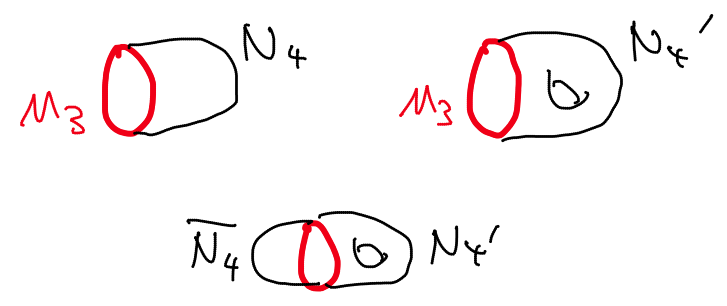
\includegraphics[width=.5\textwidth]{paste2.png}
\]
\caption{$M_3$ as a boundary and the auxiliary bounding 4-manifolds $N_4$ and $N_4'$.
\label{fig:paste2}}
\end{figure}

We now note that $[F^\text{geometric}/2\pi]$ comes from 
the first Chern class $c_1(P)\in H^2(W_4;\bZ)$ of the $U(1)$ bundle $P\to W_4$,
and in particular
\begin{equation}
\frac{1}{(2\pi)^2} \int_{W_4} F^\text{geometric}\wedge F^\text{geometric}
= \langle
c_1(P)\cup c_1(P), [W_4]
\rangle \in \bZ.
\end{equation}

This means that
the right hand side of \eqref{eq:AFdef} is well-defined modulo $(2\pi)^2$,
and therefore the following expression is well-defined for an integer $n$: \begin{equation}
\exp\left(
i\frac{n}{2\pi} \int_{M_3} A^\text{geometric}\wedge F^\text{geometric}
\right)
=
\exp\left(
\frac{i}{\hbar} \frac{n e^2}{h } \int_{M_4} A^\text{SI}\wedge F^\text{SI}
\right).
\end{equation}
Comparing with \eqref{eq:halldef}, this means that 
the partition function \eqref{eq:Zphase} is well-defined when
\begin{equation}
\sigma^\text{SI} = 2n \frac{ e^2}{h}
\end{equation}
for an integer $n$.
And this is off by a factor of 2 from the usual expression, \eqref{eq:hallquant}.

What saves the day is the following mathematical theorem:
\begin{theorem}
  \label{thm:spin-even}
  On a closed spin 4-manifold $W_4$
  and a class $a\in H^2(W_4;\bZ)$, the quantity
  \[
  \langle a\cup a, [W_4]\rangle
  \]
  is not just an integer but an even integer.
\end{theorem}


We now require all the manifolds involved, $M_3$, $N_4$, $N_4'$ and $W_4$ to be spin.
Then the right hand side of \eqref{eq:AFdef} is well-defined modulo $\alert{2}(2\pi)^2$,
and therefore for any integer $\nu$, the expressions
\begin{equation}
  \exp\left(
  i\frac{\nu}{\alert{2}\cdot 2\pi} \int_{M_3} A^\text{geometric}\wedge F^\text{geometric}
  \right)
  =
  \exp\left(
  \frac{i}{\hbar} \frac{\nu e^2}{\alert{2} h } \int_{M_4} A^\text{SI}\wedge F^\text{SI}
  \right)
  \end{equation}
is well-defined. This means that the Hall conductance should satisfy
\begin{equation}
  \sigma^\text{SI} = \nu \frac{e^2}{h}.
\end{equation}

We have thus learned that the quantization of the Hall conductance
with odd $\nu$ requires spin structures on the manifolds involved.
This is perfectly reasonable physically,
since electrons are particles with spin $1/2$,
and require spin structures on the manifolds to propagate.
Its effect on the quantization unit of the integer quantum Hall effect
is a rather indirect but intriguing consequence of this physical requirement.

\subsection{Comments}
We end this section with a few comments. 
\subsubsection{Abelian Chern-Simons terms}
We discussed in this section how to define $\int_C A$ and $\int_{M_3} A\wedge F$ 
when $A$ is not a globally-defined 1-form.
We saw that $\int_C A$ can be made well-defined modulo $2\pi$,
and that $\int_{M_3} A\wedge F$ can be made well-defined modulo $(2\pi)^2$
on orientable manifolds and modulo $2(2\pi)^2$ on spin manifolds.

In higher dimensions the natural generalizations are given by \begin{equation}
\int_{M_{2n-1}} A\wedge F^{n-1}\label{eq:abelian-CS}
\end{equation} and are known as the (abelian) Chern-Simons terms.
This term appears in various contexts in theoretical physics.
For example the next version $\int_{M_5} AF^2$ appears 
in the study of the perturbative $U(1)$ anomalies of chiral fermions in four dimensions.

Using the fact that $F/2\pi$ corresponds to $c_1$ of the $U(1)$ bundle,
it is easy to make \eqref{eq:abelian-CS} well-defined 
modulo $(2\pi)^n$ on orientable manifolds.
But we already saw that this was not enough for the quantization of the Hall conductance for $n=2$.
Similarly it is not enough if you want to apply the $n=3$ version to the study of the $U(1)$ anomalies.
It is known that, very roughly speaking, the spin structure allows us to refine the definition from modulo $(2\pi)^n$ to modulo $n! (2\pi)^n$.
But explaining it will require a lot more time than we have here.

\subsubsection{The $n=2$ case again}

In the $n=2$ case, the spin structure allowed us to reduce
 the ambiguity of the expression $\int A\wedge F$ 
from modulo $(2\pi)^2$ to modulo $2(2\pi)^2$.
Such a factor of 2 refinement of the ambiguity is known under the general name of \emph{quadratic refinement}.
In our case this relied on the mathematical fact which we quoted as Theorem~\ref{thm:spin-even}.
Here we provide what kind of algebraic topology is involved in this theorem,
by showing how this is proved. 

We want to show $\langle a\cup a, [W_4]\rangle$ is even for $a\in H^2(W_4;\bZ)$
if $W_4$ is spin.
Let $\tilde a\in H^2(W_4;\bZ_2)$ be the mod-2 reduction of $a$.
Since \begin{equation}
\langle a\cup a, [W_4]\rangle = \langle \tilde a\cup \tilde a, [W_4]\rangle \mod 2,
\end{equation}
it suffices to show that \begin{equation}
\langle \tilde a\cup \tilde a, [W_4]\rangle \equiv 0 \mod 2, 
\end{equation} 
forall $\tilde a\in H^2(W_4;\bZ_2)$
if $W_4$ is spin.

Now, it happens that there is a natural transformation \begin{equation}
\Sq^k: H^n(M;\bZ_2)\to H^{n+k}(M;\bZ_2)
\end{equation} called the Steenrod square, such that \begin{equation}
\Sq^k a_k = a_k \cup a_k
\end{equation} for $a_k\in H^k(M;\bZ_2)$.

Let $n$ be the dimension of $M$. Take  $a_{n-k}\in H^{n-k}(M;\bZ_2)$.
THen $\Sq^k a_{n-k}\in H^n(M;\bZ_2)$.
We can then consider the quantity \begin{equation}
  \langle \Sq^k a_{n-k}, [M]\rangle \mod 2.
\end{equation}
This is a linear map defined on $H^{n-k}(M;\bZ_2)$,
and therefore there should be an element $\nu_k\in H^k(M;\bZ_2)$
such that \begin{equation}
  \langle \Sq^k a_{n-k}, [M]\rangle \equiv \langle \nu_k \cup a_{n-k}, [M]\rangle \mod 2.
\end{equation}
These classes $\nu_k$ are known as the Wu classes of the manifold.
It turns out that the Wu classes can be written in terms of the Stiefel-Whitney classes of $M$.
In particular, $\nu_2(M)=w_1(M)^2 + w_2(M)$.

With this we can complete our derivation:\begin{align}
\langle \tilde a\cup \tilde a, [W_4]\rangle 
&\equiv \langle \Sq^2 \tilde a, [W_4]\rangle \\
&\equiv \langle \nu_2 \cup \tilde a, [W_4]\rangle\\
&\equiv \langle (w_1^2 + w_2) \cup \tilde a, [W_4]\rangle =0,
\end{align}
where in the last equality we used the fact that we assumed $W_4$ is spin,
which means that $w_1(W_4)=0$ from the orientability
and $w_2(W_4)=0$ from the spin condition.

\subsubsection{More general Chern-Simons terms}
The Abelian Chern-Simons terms we discussed above have the crucial property
\begin{equation}
\int_{M_{2n-1}} A\wedge F^{n-1} = \int_{M_{2n}} F^n
\end{equation} when $A$ is a globally-defined 1-form
and $M_{2n-1}=\partial M_{2n}$.
Note that the right hand side comes from the differential form expression
of a characteristic class,
and the modulo $(2\pi)^n$ ambiguity is related to the fact that 
the characteristic class is actually defined over $\bZ$. 
We also saw that we needed to reduce this ambiguity using the spin structure.

There are many other similar terms of this form.
For example, for $SU(N)$ bundles, 
the gauge curvature $F$ is a globally well-defined $N\times N$ matrix-valued 2-form,
and $\tr F^n$ is a globally well-defined $N$-form.
This is a characteristic class of the $SU(N)$ bundle,
which is actually defined over $\bZ$.
From this one can define the Chern-Simons terms $\mathrm{CS}(A)$ for $SU(N)$ bundles
as \begin{equation}
\int_{M_{2n-1}} \mathrm{CS}(A) = \int_{M_{2n}} \tr F^{n}.
\end{equation}

The tangent bundle of a manifold is an $SO(n)$ bundle
whose connection is usually denoted by $\omega$.
The curvature is the Riemannian curvature tensor, and usually denoted by $R$.
In three dimensions we then have \begin{equation}
\int_{M_3} \mathrm{CS}(\omega) = \int_{M_4} \tr R^2.
\end{equation}
$\tr R^2$ on the right hand side is (a constant multiple of)
the characteristic class $p_1$, called the first Pontryagin class.
The differential form expression on the left hand side is the gravitational Chern-Simons term.
Its presence in the effective action leads to the thermal Hall conductivity,
and the quantization of the thermal Hall conductance
follows in a similar manner 
by considering the ambiguity of the gravitational Chern-Simons term 
as we did for the abelian Chern-Simons term.

There is a crucial difference, however.
In the case of the abelian Chern-Simons term, we have the obvious property
\begin{equation}
\langle c_1(P)^2,[M_4]\rangle \in\bZ
\end{equation} for arbitrary orientable manifolds,
which was refined to \begin{equation}
  \langle c_1(P)^2,[M_4]\rangle \in 2 \bZ
\end{equation} on spin manifolds.
In the case of the gravitational Chern-Simons, 
it is fairly clear that \begin{equation}
\langle p_1(TM),[M] \rangle \in \bZ
\end{equation} since $p_1\in H^4(M;\bZ)$,
However, even on generic orientable manifolds,
we have \begin{equation}
\langle p_1(TM),[M] \rangle \in 3 \bZ.
\end{equation} 
On spin manifolds, this is further refined to \begin{equation}
\langle p_1(TM),[M] \rangle \in 48 \bZ.
\end{equation} 
And this factor of $48$ is actually necessary 
to account for the unit of quantization of the thermal Hall conductance
from this approach.


\if0
\section{K-theory}

\section{Atiyah-Singer index theorem}

\section{Anomalies}

\section{Computing \texorpdfstring{$\pi_4(S^3)$}{pi4(S3)}}
\fi

\bibliographystyle{ytamsalpha}
%\baselineskip=.85\baselineskip%\let\ttfamily\relax
%\let\bbb\bibitem\def\bibitem{\itemsep1pt\bbb}
\bibliography{ref}

\end{document}
